%%% Local Variables:
%%% mode: Xelatex
%%% TeX-master: t
%%% End:
% !TeX program = xelatex

\documentclass[draftformat,mathCMR]{HUSTthesis}%草稿用这个
%\documentclass[finalformat,mathCMR]{HUSTthesis}%盲审用这个
%\raggedbottom

\usepackage{HUSTtils}%所有其它可能用到的包都统一放到这里了,可以根据自己的实际添加或者删除。这样做主要是为了避免class文件过于臃肿。

% \setmainfont{Times New Roman}[Scale=.9]
\setmainfont{Times New Roman}
%\includeonly{body/chap02}

\begin{document}
%定义所有的eps文件在 figures 子目录下
\graphicspath{{figures/}}

% 生成封面,版权页,摘要
\frontmatter

%%% Local Variables:
%%% mode: Xelatex
%%% TeX-master: t
%%% End:

\ctitle{基于对比学习的推荐算法研究}

\xuehao{D201881076} \schoolcode{10487}
\csubjectname{信息与通信工程} \cauthorname{刘斌}
\csupervisorname{王邦} \csupervisortitle{教授}
\defencedate{2023~年~11~月~27~日} \grantdate{}
\chair{刘文予}%
\firstreviewer{A} \secondreviewer{A} \thirdreviewer{B}

\etitle{Contrastive Learning for Personalized Recommendation}
\edegree{Doctor of Engineering}
\esubject{Information and Communication Engineering}
\eauthor{LIU Bin}
\esupervisor{WANG Bang }
%定义中英文摘要和关键字
\cabstract{
在互联网飞速发展的信息时代,推荐系统在电商、社交媒体、新闻阅读等领域发挥着重要的作用。自监督推荐对输入数据进行变换或处理提取自监督信号,有助于缓解数据稀疏、虚假相关和对抗攻击等问题,受到了广泛的关注。基于对比学习的推荐算法是自监督推荐的主要实现方式,尽管在自监督设置下表现了出色的泛化能力,但与有监督设置下的对比型推荐算法存在较大差距。如何从不完整标注的数据中学到良好的特征表示,是机器学习基础理论的需要,也是提升推荐算法准确性的现实需求。

本文聚焦自监督推荐场景,针对对比型推荐算法的伪正例、伪负例和优化目标偏离问题,提出了相应的正例去噪算法、负例采样算法和损失函数校正算法。本文的创新和贡献如下:

针对伪正例问题,提出了自适应正例去噪的推荐算法。将从含噪成对比较的数据中学习排序的问题形式化为一个含有隐变量的最大后验估计问题。所提出的算法采用期望最大化框架:在期望步骤中使用贝叶斯推断来估计交互的置信度指标;在最大化步骤中固定置信度指标,更新参数学习用户和物品的特征表示。在合成的噪声数据集上表现出了更好的鲁棒性,在真实的数据集上top-5准确率相对于最优的对比算法平均提升6.2\%。

针对伪负例问题,提出了基于最优负采样准则的推荐算法。提出了后验概率意义上未标注样本是真负例的负信号测度,结合了静态的先验信息和动态的样本信息,较好地综合了现有的两种提取负信号的范式;进而提出了最优负采样准则,是经验采样风险最小化意义上的最优采样准则。该算法在采样误差率和采样样本信息量优于同类方法,相对于最优的对比算法top-5准确率平均提升3.4\%。

针对自监督设置下成对损失优化目标偏离问题,提出了基于去偏成对损失的推荐算法。通过校正伪负样本导致的概率估计偏差,修正自监督设置下成对损失的梯度,得到了去偏成对损失。该损失是有监督设置下的成对损失的一致估计,在保持严格的相对于成对学习的线性时间复杂度情况下,top-5准确率相对于最优的对比算法平均提升3.2\%。

针对自监督设置下对比损失优化目标偏离问题,提出了基于贝叶斯自监督对比损失的推荐算法。通过重要性权重来纠正从未标注数据中随机选择的负样本引入的偏差,得到了贝叶斯自监督对比损失。对于单个权重,其正比于未标注样本是真负例的后验概率估计;对于损失函数值,该损失是有监督设置下对比损失的一致估计。贝叶斯自监督对比损失可以灵活统一地执行硬负例挖掘和伪负例去偏任务,top-5准确率相对于最优的对比算法平均提升2.2\%。此外在数值仿真实验、无监督图像分类等多个任务中验证了贝叶斯自监督对比损失的有效性。

综上,本文针对自监督设置下的对比型推荐算法的三个关键组件:正例、负例和损失函数做出了改进,为后续推荐算法和对比学习研究提供了有效的支撑。
}
\ckeywords{推荐算法;对比学习;成对学习;自监督学习;负采样}

\eabstract{In the rapidly evolving information age of the Internet, recommendation systems play a crucial role in various domains such as e-commerce, social media, and news reading. Self-supervised recommendation, which leverages transformations and processing of implicit feedback data to extract self-supervisory signals, has gained significant attention due to its potential to address issues like data sparsity, false correlations, and adversarial attacks. Contrastive learning-based recommendation algorithms are the primary implementation approach for self-supervised recommendation. While they demonstrate excellent generalization capability in self-supervised settings, a significant gap exists compared to contrastive recommendation algorithms under supervised settings. Learning better feature representations from incompletely annotated data is not only a theoretical requirement for machine learning but also a practical need to enhance the accuracy of recommendation algorithms.
	
This dissertation focuses on the self-supervised recommendation scenario and addresses the issues of false positive samples, false negative samples, and optimization objective deviation in contrastive recommendation algorithms. We propose corresponding algorithms for positive example denoising, negative example sampling, and loss function correction. The innovations and contributions of this dissertation are as follows:
	
For the problem of false positive samples, we propose an adaptive denoising recommendation algorithm for learning personalized ranking from noisy implicit feedback data. We formalize the problem of learning ranking from noisy pairwise comparison data as a maximum a posteriori estimation problem with latent variables. The proposed algorithm adopts an Expectation-Maximization framework: in the Expectation step, Bayesian inference is used to estimate confidence indicators for interactions, and in the Maximization step, the confidence indicators are fixed to update the feature representations of users and items. The algorithm demonstrates better robustness on synthetic noisy datasets and achieves an average improvement of 6.2\% in top-5 precision compared to the optimal baseline algorithm on real datasets.
	
For the problem of false negative samples, we propose a recommendation algorithm based on the optimal negative sampling criterion. We introduce a negative signal measurement in terms of posterior probability, combining static prior information and dynamic sample information, effectively integrating the two main paradigms for extracting negative signals. This approach provides a flexible interface for modeling prior probabilities using auxiliary information. Furthermore, we propose the optimal negative sampling criterion, which is the theoretically optimal sampling rule in terms of empirical sampling risk minimization. The algorithm outperforms similar methods in terms of sampling error rate and sampling sample information. It achieves an average improvement of 3.4\% in top-5 precision compared to the optimal baseline algorithm.
	
For the problem of optimization objective deviation of pairwise loss, we propose a recommendation algorithm based on debiased pairwise loss. By correcting probability estimation biases caused by false negative samples, we approximate the gradient to approximate the gradient of pairwise loss under supervised settings, resulting in a debiased pairwise loss. This loss provides a consistent estimation of the pairwise loss under supervised settings without the need for side information for supervision. Based on the debiased pairwise loss, The algorithm achieves an average improvement of 3.2\% in top-5 precision compared to the optimal baseline algorithm, while maintaining linear time complexity relative to BPR.
	
For the problem of optimization objective deviation of contrastive loss, we propose a recommendation algorithm based on Bayesian self-supervised contrastive loss. By using importance weights to correct biases introduced by randomly selected negative samples from unlabeled data, we obtain the Bayesian self-supervised contrastive loss. For the individual weight, it is proportional to the posterior probability estimate that the unlabeled sample being true negative, allowing flexible execution of hard negative mining and false negative sample debiasing tasks. From a numerical perspective, this loss provides a consistent estimation of the supervised contrastive loss, thereby improving the generalization performance of recommendation models. It achieves an average improvement of 2.2\% in top-5 precision compared to the optimal baseline algorithm. Furthermore, the effectiveness of the Bayesian self-supervised contrastive loss is further verified in numerical experiments and  un-supervised image classification task.
	
In conclusion, this dissertation proposes improvements for three key components of contrastive recommendation algorithms in self-supervised settings: positive examples, negative examples, and loss functions. These improvements provide effective support for future recommendation algorithms and contrastive learning research. }

\ekeywords{Recommender System, Contrastive Learning, Pairwise Learning, Self-supervised Learning, Negative Sampling}

\makecover
%目录
\tableofcontents
\listoffigures
\listoftables

% 对照表
%\begin{denotation}
\item[自监督学习] Self-supervised learning
\item[监督学习] Supervised learning
\item[无监督学习]  Un-supervised learning
\item[成对学习]  Pairwise learning
\item[对比学习] Contrastive learning (CL)
\item[正例未标注] Positive-unlabeled (PU)
\item[困难负例] Hard negative sample
\item[伪负例] False negative sample (FN)
\item[真负例] True negative sample (TN)
\item[伪正例] False positive sample (FP)
\item[负采样] Negative sampling 
\item[噪声对比估计] Noisy contrastive estimation (NCE)
\item[概率密度函数] Probability density function (PDF)
\item[类条件概率密度] Class conditional probability density 
\item[累计分布函数] Cumulative distribution function (CDF)
\item[经验分布函数] Empirical cumulative distribution function (eCDF)
\item[极大似然估计] Maximum likelihood estimation (MLE)
\item[最大后验估计] Maximum a posteriori estimation (MAP)
\item[贝叶斯个性化排序] Bayesian personalized ranking (BPR)
\end{denotation}
  
\chapter*{中英文缩写对照表}
\begin{center} \xiaosi
\vspace{2.0cm}
\renewcommand{\arraystretch}{1.5}
\begin{longtable}{|l|l|l|}
\hline
\textbf{英文缩写}& \textbf{英文全称}&\textbf{中文全称} \\\hline
SSL&Self-Supervised Learning& 自监督学习  \\\hline
SL&Supervised Learning & 监督学习\\\hline
UL&UnSupervised Learning& 无监督学习\\\hline
PL&Pairwise Learning&  成对学习\\\hline
CL&Contrastive Learning & 对比学习 \\\hline
PU&Positive-Unlabeled& 正例未标注 \\\hline
HN&Hard Negative Sample&困难负例\\\hline
FN&False Negative Sample& 伪负例 \\\hline
TN&True Negative Sample& 真负例 \\\hline
FP&False Positive Sample& 伪正例 \\\hline
NS&Negative Sampling& 负采样 \\\hline
NCE&Noisy Contrastive Estimation& 噪声对比估计 \\\hline
PDF&Probability Density Function&  概率密度函数\\\hline
CCPD&Class Conditional Probability Density& 类条件概率密度 \\\hline
CDF&Cumulative Distribution Function&累计分布函数 \\\hline
eCDF&Empirical Cumulative Distribution Function& 经验分布函数 \\\hline
MLE&Maximum Likelihood Estimation& 极大似然估计 \\\hline
MAP& Maximum Posteriori Estimation&最大后验估计 \\\hline
BPR&Bayesian Personalized Ranking&  贝叶斯个性化排序\\\hline
\end{longtable}
\end{center}  

\mainmatter
%%% mode: latex
%%% TeX-master: t
%%% End:

\chapter{绪论}
\label{cha:intro}

\section{研究背景与意义}\label{sec:general intro}
推荐系统\cite{rs}是互联网信息时代解决信息过载问题的重要工具。其通过分析用户行为数据和历史行为信息,提供相关性、多样性和新颖性的内容选择,帮助用户快速准确地找到感兴趣的信息、辅助用户做出更明智的决策。在互联网飞速发展的信息时代,推荐系统在电商、社交媒体、新闻阅读等领域发挥着重要的作用,逐渐成为学术界和工业界的研究热点\cite{Steffen:2009:UAI,Ai:2018:SIGIR,Ding:2020:NIPS}。

%推荐系统广泛使用了自监督学习的技术。受限于推荐系统的场景特征,获取准确的用户偏好标签用于训练推荐模型是昂贵的。目前许多最先进的推荐模型都借助于自监督学习(Self-supervised Learning, SSL)\cite{Liu:2021:TKDE}的技术,通过对输入数据进行某种变换或处理来提取自监督信号。常见的自监督信号例如“用户对已交互的物品偏好大于未交互物品”\cite{Steffen:2009:UAI,Jingtao:2019:IJCAI,Xiangnan:2020:SIGIR,Wang:2019:SIGIR},“用户物品二分图轻微扰动的语义不变性”\cite{shuai2022review,lightgcl:2023:ICLR,wu:2023:TKDE}等。这种使用自监督信号的训练的推荐模型也被称为自监督推荐\cite{SSR:2023:TKDE}(Self-supervised Recommendation, SSR),是自监督学习的一个重要应用领域。自监督推荐分利用输入数据中的内在关系设计自监督任务训练推荐模型,不仅可以减少对手动标注数据集的依赖,而且也有助于缓解传统推荐系统中的数据稀疏、虚假相关性和对抗性攻击等问题\cite{SSR:2023:TKDE,Liu:2021:TKDE}。

推荐系统广泛使用了自监督学习的技术\cite{SSR:2023:TKDE,Xiangnan:2020:SIGIR,Wang:2019:SIGIR,shuai2022review,guo2022miss,tao2022self,yao2021self,xia2021self,liu2021contrastive,yuan2021improving,wu2020ptum,ma2020disentangled,10.1145/3459637.3482426,10.1145/3404835.3462862,self:aug}。受限于推荐系统的场景特征,获取准确的用户偏好评分标签是昂贵的。目前许多最先进的推荐模型都借助自监督学习(Self-supervised Learning, SSL)\cite{tong2023emp,Liu:2021:TKDE,Chen:2020:NIPS,BYOL:2020:NIPS,wu:2023:TKDE,gsl:2023:TKDE}技术,设计自监督任务(预)训练模型编码用户物品特征表示,以预测个性化排序(下游任务)。例如,生成型(Generative)自监督任务训练推荐模型对输入数据进行重建\cite{sun2019bert4rec,geng2022recommendation,zhang:sigir};对比型(Contrastive)自监督任务训练推荐模型编码正负样本差异特征\cite{Steffen:2009:UAI,Jingtao:2019:IJCAI,Xiangnan:2020:SIGIR,Wang:2019:SIGIR,shuai2022review,lightgcl:2023:ICLR,wu:2023:TKDE}。这种基于自监督任务引导训练的推荐模型也被称为自监督推荐\cite{SSR:2023:TKDE}(Self-supervised Recommendation, SSR),是自监督学习的一个重要应用领域。自监督推荐充分利用输入数据中的内在关系提取自监督信号,不仅可以减少对手动标注数据集的依赖,而且也有助于缓解传统推荐系统中的数据稀疏、虚假相关性和对抗性攻击等问题\cite{SSR:2023:TKDE,Liu:2021:TKDE}。

基于对比学习(Constrastive Learning, CL)\cite{zhang:cl}的推荐算法是自监督推荐的主要实现形式\cite{SSR:2023:TKDE},也称为对比型推荐算法。推荐系统中常见的对比方式包括“已交互的物品偏好大于未交互物品”的偏好对比\cite{Steffen:2009:UAI,Jingtao:2019:IJCAI,Xiangnan:2020:SIGIR,Wang:2019:SIGIR},“图轻微扰动语义不变性”的图对比\cite{shuai2022review,lightgcl:2023:ICLR,wu:2023:TKDE}等。对比学习在计算机视觉、自然语言处理和信息检索领域取得了巨大的成功\cite{Oord:2018:arxiv,Chen:2020:ICML,BYOL:2020:NIPS,Khosla:2020:NIPS,graph:CL,graph:self,cl:bei,xiao:cl},在推荐任务中也有诸多优势,主要体现在:(1) 互信息优化:通过
优化对比损失,拉近锚点与正例的距离、推远锚点与负例的距离,实现对互信息的优化\cite{Oord:2018:arxiv,yang2021enhanced,cao2021bipartite,zhou2020s3}。(2) 避免过拟合:对比损失激励编码器编码不同样本的差异特征,免于对样本进行像素级信息重构,从而避免了模型的过拟合\cite{Oord:2018:arxiv}。(3) 排序导向:在偏好对比任务中,优化成对损失或对比损失,导致了对排序列表排序指标AUC和NDCG的优化\cite{Steffen:2009:UAI,Jiancan:2022:arxiv}。

%
%对比学习\cite{zhang:cl}是自监督推荐的主要实现形式\cite{SSR:2023:TKDE}。对比学习在计算机视觉、自然语言处理和信息检索领域取得了巨大的成功\cite{Oord:2018:arxiv,Chen:2020:ICML,BYOL:2020:NIPS,Khosla:2020:NIPS}。对比学习在推荐任务中也有诸多优势,主要体现在:(1) 互信息优化:通过
%优化对比损失,拉近锚点与正例的距离、推远锚点与负例的距离,实现对互信息的优化\cite{Oord:2018:arxiv,yang2021enhanced,cao2021bipartite,zhou2020s3}。(2) 避免过拟合:对比损失激励编码器编码不同样本的差异特征,免于对样本进行像素级信息重构,从而避免了模型的过拟合\cite{Oord:2018:arxiv}。(3) 排序导向:在“用户对已交互物品的偏好大于为交互物品”这个的对比任务中,优化成对损失或对比损失,导致了对排序列表排序指标AUC和NDCG的优化\cite{Steffen:2009:UAI,Jiancan:2022:arxiv}。


基于对比学习的推荐算法显著推动了自监督推荐的前沿\cite{SSR:2023:TKDE},受到了广泛的关注\cite{liu2021contrastive,10.1145/3477495.3532009,qiu2022contrastive,yu2023xsimgcl}。尽管该类方法在自监督设置下表现出了出色的泛化能力,\textbf{但与有监督设置下的对比型推荐算法存在较大差距}\cite{Chuang:2020:NIPS,SSR:2023:TKDE,Khosla:2020:NIPS,zhang:cl}:用于偏好对比的正负样本标签是“伪标签”\footnote{自监督学习和无监督学习的共性是都不涉及人工标注的标签\cite{He:2020:CVPR};区分在于,自监督学习通过从共现输入中导出“伪标签”来关联信息\cite{Liu:2021:TKDE}。},不同于“喜欢与否”的真实偏好标签。二者的不一致性,对学习准确的用户物品特征表示产生不利影响。如何从不完全标注的隐式反馈数据中学到良好的对比表示(Contrastive Representations),是自监督学习和对比学习的理论需要,也是提升个性化推荐系统准确性的现实需求。

\section{国内外研究现状}
\label{sec:requirement}
现实世界中,对样本的度量方式主要有两种,一是对样本进行逐个(Pointwise) 度量,例如测量电容的大小。在高自由度场景中,由于:(1)单个样本的绝对值度量不容易获取;(2)体现相互关系的度量只能以成对方式体现;(3)特定场景中更关注相对值的大小而非绝对值的大小,导致了成对(Pairwise)度量的出现。成对度量广泛存在于描述客观世界的数据中,度量的方式主要有:(1)成对比较,例如方案$i$比方案$j$好,体现的是强弱关系;(2)成对关系,例如网页$i$的超链接指向网页$j$,体现了相互依存和作用的关系。成对度量提供了从相互关系描述、分析、挖掘事物的视角,相比于逐个度量的方式,突出了数据内部的结构信息,能够更好地描摹客观世界的真实形态。

\vspace{-0.0011cm}
推荐系统通常收集到的数据是隐式反馈数据,如点击、购买、浏览等行为数据。贝叶斯个性化排序 (Bayesian Personalized Ranking, BPR)\cite{Steffen:2009:UAI}率先将隐式反馈数据转化为成对比较。具体而言,对于某个用户(锚点),已交互物品$i$被标记为正例,未交互的物品$j$被标记为负例,相应的正负例构成一个成对比较实例。基于“用户对正例偏好大于负例的偏好”的假设(自监督信号),BPR使用Bradley-Terry模型\cite{Bradley:1952:Biometrika,Luce:2005:JASA}建模成对比较的似然,并通成对比较的极大似然估计学习潜在的用户表示和物品表示,在推荐中被称为成对学习\cite{Steffen:2009:UAI,Steffen:2014:WSDM,Xiangnan:2020:SIGIR,Wang:2019:SIGIR}。这种由偏好对比引导的模型(预)训练任务,激励推荐模型给正例评分大于负例,从而导致了排序列表的AUC指标的优化\footnote{如不考虑正则化项,成对损失函数BPR与AUC指标定义相同,不同之处在于BPR把AUC指标中不可微的$0-1$损失$\ell_{0-1}(\cdot)$替换成了可微的替代损失$\log\sigma(\cdot)$\cite{Steffen:2009:UAI}。}。由于BPR设计的偏好对比与下游排序预测任务具有一致性,逐渐主导了从隐式反馈数据中学习排序的任务\cite{Weike:2013:IJCAI,Yu:2018:CIKM,Xiaoye:2011:MathProg,Xuejiao:2020:ASC,Qiu:2018:IS,Zhao:2019:FGCS}。

\vspace{-0.0011cm}
成对学习BPR根植于对比学习范式\cite{Xu:2022:arxiv}。特别是,BPR损失与噪声对比估计\cite{Gutmann:2010:ICAIS,gutmann:2012:JMLR}(Noisy Contrastive Estimation, NCE)损失具有完全等价的函数形式\cite{Liu:2021:TKDE},它们都是广泛使用的对比损失InfoNCE\cite{Oord:2018:arxiv}在负例个数设置为1时的特例。尽管它们的解释不同,BPR将优化目标解释为用户偏好正例强于负例的后验,InfoNCE将优化目标解释为从负例中区分出正例的后验,但实际上都描述了由模型参数化的正例得分大于负例得分的程度。随后,InfoNCE损失也广泛应用于推荐中的排序预测任务\cite{Jiancan:2022:arxiv,lightgcl:2023:ICLR}。文献\cite{Jiancan:2022:arxiv}进一步讨论了优化InfoNCE损失导致优化排序指标NDCG。

\vspace{-0.0011cm}
对比学习采用从比较中学习(learn-to-compare)\cite{Gutmann:2010:ICAIS}的范式,通过区分观察数据和噪声数据来使模型免于重建数据的像素级信息~\cite{Oord:2018:arxiv}。虽然表示编码器和相似性度量会因任务而异~\cite{Devlin:2018:bert,He:2020:CVPR,Dosovitskiy:2014:NIPS,Xiangnan:2020:SIGIR,Wang:2019:SIGIR,Wenqi:2021:KDD},但它们都共享将正样本和负样本进行对比的基本思想,通过优化对比损失~\cite{Wang:2020:ICML}来训练编码器,如NCE损失~\cite{Gutmann:2010:ICAIS},InfoNCE损失~\cite{Oord:2018:arxiv},Infomax损失~\cite{Hjelm:2018:Arxiv},渐进对比损失~\cite{Wang:2020:ICML}等。这些损失函数隐式~\cite{Oord:2018:arxiv}或显式~\cite{Hjelm:2018:Arxiv}地优化了已知数据和待预测数据互信息的下界。Arora等人~\cite{Saunshi:2019:ICML}为对比学习的泛化界限提供了理论分析。对比学习在不同领域的许多应用中都取得了显著成功~\cite{Henaff:2020:ICML,Khosla:2020:NIPS,Liu:2021:TKDE,Bachman:2019:NIPS,chen2020improved,Huang:2019:ICML,Wu:2018:CVPR,Zhuang:2019:CVPR}。除了互信息优化、防止模型过拟合等优势之外,对比学习在推荐任务中的突出优势体现在推荐任务和对比学习任务的一致性\footnote{这里的一致性是指,由成对损失和对比损失引导的预训练任务((Pretext Task)与下游排序预测任务是一致的,体现在预训练阶段的对比损失和下游任务的性能度量存在关联。}:优化对比损失导致排序列表排序指标的优化\cite{Steffen:2009:UAI,Jiancan:2022:arxiv}。

\vspace{-0.0011cm}
从对比学习的视角,后续的研究按照对比学习的关键组件可以归纳为,正例增强方法,负例采样方法,对比损失函数设计等工作。正例增强主要通过附属信息获取不同偏好强度的正例\cite{Qiu:2018:IS,Lerche:2014:RS,Wenhui:2019:WWW,Yu:2018:CIKM,Bin:2020:IS}构造更细粒度的偏好比较,以学习更准确的决策边界。由于附属信息有限,后续的工作设计了基于图增强的图对比任务提升学到的表示\cite{lightgcl:2023:ICLR,ren2023disentangled,he2023candidate,yang2023generative};
%通过对比原图和增强图,学习体现用户物品二分图中重要的结构信息的节点特征表示\cite{lightgcl:2023:ICLR,ren2023disentangled,he2023candidate,yang2023generative};
负例的采样方法围绕采样困难负样本\cite{Steffen:2014:WSDM,Zhang:2013:SIGIR,Zhao:2015:CIKM,shi2023theories},且避免采样伪负样本\cite{Ding:2020:NIPS,Qin:2021:AAAI,Zhao:2021:IJCAI,Chen:2017:KDD,Mikolov:2013:NIPS,Weike:2013:IJCAI,Yu:2018:CIKM,Wang:2019:SIGIR}这两个目标展开,以激励模型更准确地学习兴趣边界。在损失函数设计上,主要是将排序导向的偏好对比任务和图对比任务组合,将原始的单一对比目标向多个对比目标进行拓展,使得最终的优化目标同时约束排序目标和保留用户物品二分图结构信息的目标\cite{Wang:2022:KDD,ren2023disentangled,lightgcl:2023:ICLR,he2023candidate,zhu2023adamcl,qin2023meta,shuai2022review}。


\section{关键问题}
在推荐系统中,正例的语义为“喜欢的物品”,负例的语义为“不喜欢的物品”。然而,用户通常只通过交互行为(如点击、购买)来表达偏好或兴趣。一方面,这些交互行为通常不包含显式的评分,只能观测到交互的有无,无法观测到交互数据所对应的偏好强度高低。不体现偏好的交互如代购、误触、查看等异常模式与正常交互无法区分,都被标记为正例\cite{Yu:2018:CIKM,Qiu:2018:IS,Wang:2021:WSDM}。另一方面,由于用户仅仅提供正反馈,无法观测到用户不喜欢哪些物品,所有用户未看见的物品都被标记为负例,但它们实际上是未标注数据\cite{Ding:2020:NIPS,Zhang:2013:SIGIR,Yang:2020:KDD}。因此,用于训练推荐系统的数据集通常以正例-未标注(Positive-Unlabeled, PU)形式存在,且正例还含有噪声。依照隐式反馈数据交互的有无获取的正负样本的“伪标签”,与真实的偏好标签具有不一致性。这一现象,导致自监督设置下的对比型推荐算法存在以下问题:
\begin{enumerate}
\item \textbf{伪正例问题}

~~~~~~~~正例(已交互物品)不代表正面偏好。一些异常交互模式,如代购、误触、查看等交互数据,不体现用户偏好,但是和其它正常交互被无差别记录,构成了伪正例问题。其含义为真实标签为负例,但被标记为正例\cite{ml:2018}。伪正例问题源于隐式反馈数据的不完全性,只能观测到交互的有无,无法观测到偏好标签的大小。基于伪正例构造的“用户对已交互物品偏好大于未交互物品的偏好”的错误自监督信号,可能导致模型对数据的过拟合。模型可能会将伪正例视为用户真实的偏好模式,从而导致错误的学习和预测\cite{Han:2018:NIPS,Arpit:2017:ICML}。更具体地,模型将伪正例当作用户喜欢的物品,协同过滤机制会导增加推荐与伪正例类似的物品,从而导致top-k推荐列表中过高的伪正例率。

\item \textbf{伪负例问题}

~~~~~~~~负例(未交互物品)不代表负面偏好。未交互物品大部分是用户没有看见的物品,这些未标注物品中,包含用户潜在感兴趣的物品,即伪负例。其含义为真实标签为正例,但被标记为负例\cite{ml:2018}。伪负例问题也是源于隐式反馈数据标注的不完全性。依交互与否自动标记得到的负例,与用户不喜欢的负例的分布存在差异,模型无法准确地捕捉负例的真实分布和模式\cite{gutmann:2012:JMLR},从而导致预测结果的不可靠性。这些伪负例会导致模型误判用户不喜欢此类物品,协同过滤机制减少推荐与伪负例类似的物品,从而导致top-k推荐列表过低的真正例率。

\item \textbf{成对学习优化目标偏离问题}

~~~~~~~~在完全监督设置下,成对学习的优化目标是排序列表AUC风险的无偏估计,因此成对学习与排序预测任务是一致的:最小化成对损失将导致排序列表AUC指标最大化\cite{Steffen:2009:UAI}。在负例无监督情况下,把未标注样本当作负例计算的成对损失优化目标不再是排序列表AUC风险的无偏估计,从而偏离了完全监督设置下的成对优化目标。从单个成对比较来看,成对学习优化了有偏的“用户喜欢正例大于负例”的似然,从而对排序任务产生不利影响。

\item \textbf{对比学习优化目标偏离问题}

~~~~~~~~在完全监督设置下,对比学习的优化目标含义是从负例中分类出正例的交叉熵。在负例无监督情况下,任何未标注样本都被标记为负例。此时正负类别的语义与完全监督下类别的语义发生偏离,一方面使得优化目标不再是“从负例中区分出正类的交叉熵”,从而偏离了完全监督设置下的对比学习优化目标\cite{Chuang:2020:NIPS,Li:2021:ICLR};另一方面,推荐模型训练和下游任务关于负样本类别语义的不一致性,对推荐模型的泛化性能产生负面影响。
\end{enumerate}



\section{研究内容}
本文聚焦于自监督推荐场景,针对比型推荐算法的伪正例、伪负例和优化目标偏离问题,提出了相应的正例去噪算法、负例采样算法和损失函数校正算法,并且将损失函数校正方法从只有一个负例的成对学习向更具一般性的多个负例的对比学习推广。图\ref{1Fig:content}展示了本文的研究内容和关键问题的关系。
%*******************************
\begin{figure*}[!]
	\centering
	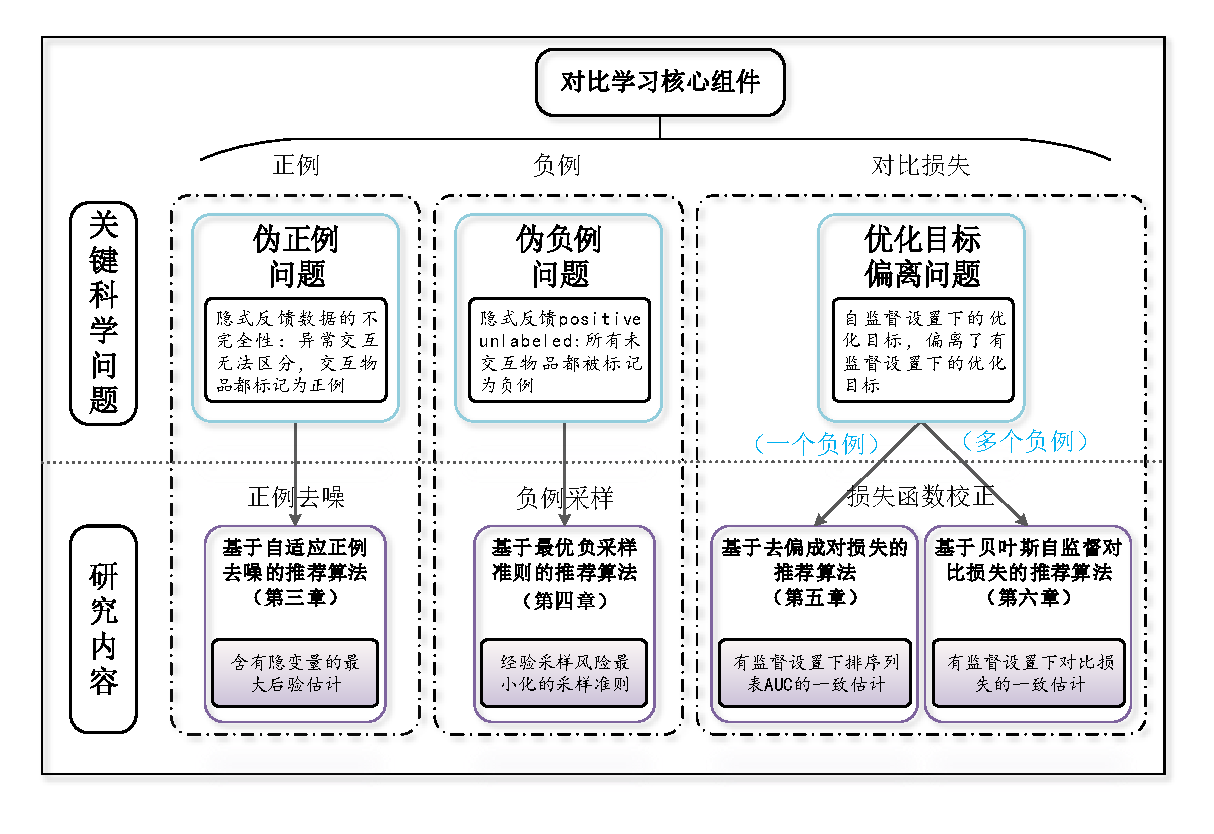
\includegraphics[width=\textwidth]{content.pdf}
	\caption{关键问题与研究内容的关系}
	\label{1Fig:content}
\end{figure*}
%*******************************

\textbf{1)自适应去噪的成对排序推荐算法}


针对伪正例问题,分析了隐式反馈的本质是不完全数据(Incomplete Data),并把从含噪成对比较的数据中学习排序的问题形式化为一个含有隐变量的最大后验估计问题。引入一个隐变量作为衡量交互置信度的新指标,这个隐变量与用户物品的特征表示一起作为模型参数一起端到端地学习。所提出的算法采用期望最大化框架:在期望步骤中使用贝叶斯推断来估计交互的置信度指标;在最大化步骤中固定置信度指标,更新参数学习用户和物品的特征表示。该算法在合成的噪声数据集上表现出了更好的鲁棒性,在真实的数据集上表现出更高的推荐准确性。


\textbf{2)基于最优负采样准则的推荐算法}


针对伪负例问题,提出了最优负采样准则,用于从未标记的数据中采样高质量的负例,以提升对比学习的训练效果并提升推荐精度。提出了后验概率意义上的负信号测度,用于度量未标记样本是真负例的概率。它使用了静态的先验信息和动态的样本信息,较好地综合了现有的两种提取负信号的两种主要范式,并为使用辅助信息建模先验概率的方法提供了灵活的接口。而后提出了最优负采样规则,这是最小化经验采样风险的理论最优的采样准则。该负采样算法在采样误差率和采样样本信息量以及推荐准确性上优于同类方法。


\textbf{3)基于去偏成对损失的推荐算法}


针对自监督设置下成对学习优化目标偏离问题,提出了去偏成对损失,通过校正伪负样本导致的概率估计偏差,从而修正梯度以近似完全监督数据的梯度。去偏成对损失是有监督设置下的成对损失的一致估计,以提升推荐模型的泛化性能。所提出的目标函数不需要额外的辅助信息进行监督,也不需要过多的存储和计算开销。在保持严格的相对于成对学习的线性时间复杂度情况下,基于去偏成对损失的推荐算法取得了更高的推荐准确性。


\textbf{4)基于贝叶斯自监督对比损失的推荐算法}


针对自监督设置下对比学习优化目标偏离问题,提出了贝叶斯自监督对比损失,通过重要性权重来纠正从无标签数据中随机选择的负样本引入的偏差。从单个权重来看,它是未标注样本为真负例的后验概率估计,可以灵活统一地执行硬负例挖掘和伪负例去偏任务这两个矛盾的任务。从损失函数的数值来看,贝叶斯自监督对比损失是有监督设置下的对比损失的一致估计,从而提升推荐模型的泛化性能。只需修改对比损失函数,并且无需额外的存储和计算开销,基于贝叶斯自监督对比损失的推荐算法取得了更高的推荐准确性。此外,在数值实验、图像分类等任务上也验证了贝叶斯自监督对比损失的有效性。

本文共分七章,第一章绪论部分主要介绍了研究背景及意义。第二章介绍了自监督推荐算法和对比学习的基础理论与相关工作。第三、四、五、六章介绍主要研究内容。第七章对全文进行总结,并指出存在的问题及未来可能的发展方向。





%%% mode: latex
%%% TeX-master: t
%%% End:

\chapter{基础理论与相关工作}
\label{cha:intro1}
%对比学习是自监督学习的重要途径,在计算机视觉、自然语言处理等诸多领域取得了瞩目的成就,推荐算法也根植于这一范式。正样本增强、负样本采样、损失函数设计,是对比学习的核心组件,也是提升推荐性能的关键途径。本章首先介绍对比学习的基本概念,并分析了推荐中的主流方法成对学习与对比学习的联系。然后介绍对比的研究现状,包括正样本的数据增强、负样本采样、网络架构设计以及损失函数设计。最后,介绍本文会使用到的一些重要的预备知识。

不完全标注的隐式反馈数据是制约推荐模型充分发挥潜力的瓶颈。自监督学习(SSL)\cite{Liu:2021:TKDE}作为一种学习范式,充分利用输入数据中的内在关系提取监督信号,可以减少对手动标签的依赖,广泛应用于推荐系统中最先进的推荐模型。本章首先从自监督学习的角度对推荐系统的现有工作进行梳理。其次对自监督推荐的主要途径--对比学习基础理论与相关工作进行介绍,并着重分析了成对损失BPR和对比损失InfoNCE之间的理论关联。最后,介绍本文会使用到的一些重要的预备知识。

\section{推荐算法相关工作}
近年来,借助深度神经网络模型的强大拟合能力和泛化性能,推荐系统取得了巨大的成功。然而,基于深度神经网络模型的推荐模型需要大量的训练数据。与可以通过众包完成的图像注释任务不同,推荐系统中的数据获取成本很高,因为个性化推荐依赖用户自身生成的数据,需要准确标注用户对海量物品的喜欢/不喜欢程度,才能使得推荐模型准确捕捉用户的偏好,从而产生准确的推荐。然而,大多数用户通常只与众多物品中的一小部分进行交互\cite{Steffen:2009:UAI,Zhang:2013:SIGIR}。因此,隐式反馈数据的稀疏性和标注不完全性问题成为制约深度推荐模型充分发挥潜力的瓶颈\cite{Zhang:2020:ACM}。

自监督学习(SSL)\cite{Liu:2021:TKDE}充分利用输入数据中的内在关系,通过对输入数据进行某种变换或处理提取监督信号,可以减少对手动标签的依赖,受到了相当大的关注。自监督学习的基本思想是通过精心设计的预训练任务(Pretext Task),例如对比语义相同的对象,从无标签数据中提取可迁移的知识。由于自监督学习有助于缓解服广泛存在的标签不足问题,已广泛应用于计算机视觉\cite{He:2020:CVPR,BYOL:2020:NIPS,Chen:2020:ICML},自然语言处理\cite{Devlin:2018:bert},音频表示学习\cite{Oord:2018:arxiv},图学习\cite{GCC:2020:KDD,velivckovic2018deep}等诸多领域。最新的基于自监督学习的方法甚至在许多计算机视觉(CV)和自然语言处理(NLP)任务中表现出与有监督模型相当的性能\cite{Robinson:2021:ICLR,Chuang:2020:NIPS,BYOL:2020:NIPS}。由于推荐系统的数据集标签不足,且受到自监督学习在其他领域取得的巨大成功的启发,目前已经有大量的研究探索将自监督学习应用于推荐领域。

自监督推荐(Self-Supervised  Recommendation,  SSR)模型为克服推荐系统中的数据稀疏问题提供了一种新的途径。本文综合文献\cite{Liu:2021:TKDE,SSR:2023:TKDE}的归纳,总结了自监督推荐(SSR)的三个关键特征如下:
\begin{enumerate}
\item \textbf{半自动地利用原始数据本身进行标注}。自监督推荐充分利用输入数据中的内在关系,通过对输入数据进行某种变换或处理来创建“伪标签”。例如BPR\cite{Steffen:2009:UAI}将交互的物品自动标记为正例,而未交互的物品标记为负例,就是执行自动化标注过程。需要注意的是,自动标注的标签是伪标签,不同于用户喜欢与否的真实偏好标签。

\item \textbf{通过提取自监督信号对推荐模型进行(预)训练的任务}。常见的自监督信号如“用户对正例的偏好强于负例”\cite{Steffen:2009:UAI},目的在于训练模型对正例的评分大于负例;另外一种常见的自监督信号是“用户物品二分图轻微扰动的语义不变性”\cite{lightgcl:2023:ICLR},目的在于训练推荐模型学习到用户物品二分图的结构信息。

\item \textbf{自监督任务旨在提升推荐性能,而非作为最终目标}。自监督任务引导的模型(预)训练阶段是为了编码用户物品的特征表示,与个性化推荐(下游任务)不一定一致。这一特征强调了推荐任务和自监督任务之间的主辅关系,学习良好的用户物品特征表示,是为了产生更准确的个性化推荐结果。例如,基于“用户对正例的偏好强于负例”的自监督信号设计的偏好对比任务,目标是激励推荐模型对正例评分大于负例评分,与推荐任务是一致的\cite{Steffen:2009:UAI,Jiancan:2022:arxiv}。而基于“用户物品二分图轻微扰动的语义不变性”这个自监督信号设计的图对比任务,目标是学习用户物品二分图的结构信息,与推荐任务不一致。因此图对比任务通常与偏好对比任务联合优化,并通过线性组合控制不同任务的主次\cite{10.1145/3543507.3583251,lightgcl:2023:ICLR}。
\end{enumerate}

推荐系统中涉及的自监督任务是多样的。根据自监督任务的性质,可以将现有的自监督推荐模型分为三种主要类型:对比型推荐算法、预测型推荐算法、生成型推荐算法。下文对这三种主要的自监督推荐算法进行介绍。
\vspace{-0.0011cm}
\subsection{对比型推荐算法}
\vspace{-0.0011cm}
典型的对比型推荐算法如图~\ref{2Fig:self1}所示,旨在通过拉近正样本对、推远负样本对,从而编码不同类别样本的差异特征。根据对比的目标不同,对比型推荐算法可以分为排序导向的偏好对比,和学习图结构信息导向的图对比。
%*******************************
\begin{figure*}[!]
	\centering
	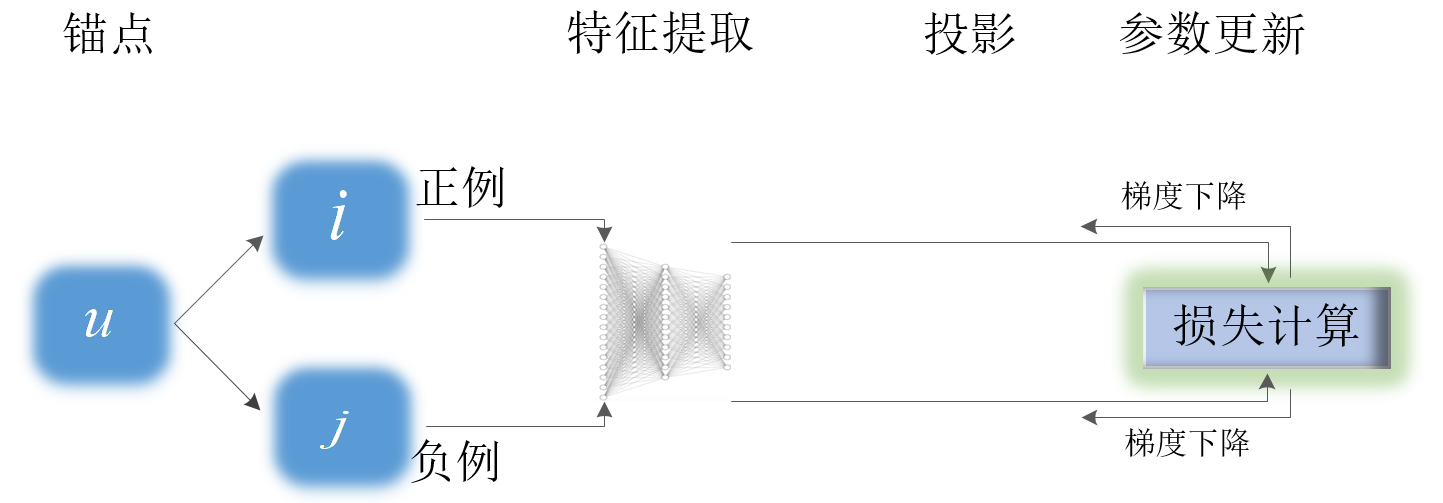
\includegraphics[width=0.8\textwidth]{self1.png}
	\caption{典型的对比型推荐算法示意图}
	\label{2Fig:self1}
\end{figure*}
%*******************************
\subsubsection{偏好对比}
偏好对比的自监督信号主要来自于用户对已交互物品的偏好大于未交互物品的偏好,开创性工作是成对学习BPR\cite{Steffen:2009:UAI},核心思想是通成拉近用户喜欢的正样本、推远用户不喜欢的负样本学习潜在的用户表示和物品表示。在偏好对比任务下,正样本的语义为用户喜欢的物品,负样本的语义为用户不喜欢的物品。这种基于偏好对比引导的模型(预)训练任务,激励推荐模型给正例评分大于负例,导致了排序列表的AUC指标的优化\cite{Steffen:2009:UAI}。随后InfoNCE损失\cite{Oord:2018:arxiv}也被广泛应用于偏好对比。文献\cite{Jiancan:2022:arxiv}揭示了在偏好对比任务下,优化InfoNCE损失有助于硬负例挖掘、缓解流行度偏差,并且优化排序列表的NDCG指标。由于BPR设计的偏好对比与下游排序预测任务具有一致性,逐渐主导了从隐式反馈数据中学习排序的任务\cite{Steffen:2014:WSDM,Xiangnan:2020:SIGIR,Wang:2019:SIGIR}。


偏好对比的后续的工作,主要是通过一些附属信息将正负样本对的概念进行拓展,构造了更具细粒度的偏好比较\cite{Weike:2013:IJCAI,Yu:2018:CIKM,Xiaoye:2011:MathProg,Xuejiao:2020:ASC,Qiu:2018:IS,Zhao:2019:FGCS}。例如,被购买的物品比只被浏览的物品更受用户喜欢\cite{Qiu:2018:IS};多次交互的物品比只有一次交互的物品更受用户喜欢\cite{Lerche:2014:RS};用户未看到过的物品应该比曝光给用户但没有交互的物品更受喜欢\cite{Wenhui:2019:WWW,Yu:2018:CIKM,Bin:2020:IS}。这些拓展的偏好比较实际上是通过附属信息提取了更密集和更可靠的自监督信号,有助于学习用户更具细粒度的偏好特征。


\subsubsection{图对比}
图(Graph)对比的自监督信号主要来自于用户物品二分图轻微扰动的语义不变性。在图对比任务下,正样本的语义为原图和增强图中的相同节点,负样本的语义为原图和增强图中的不同节点,目标是学习体现图结构信息的表示,与推荐任务不一致。根据对比的对象,遵循文献\cite{wu:2023:TKDE,gsl:2023:TKDE}提出的分类,图对比任务可以分为三种类型:结构级对比、特征级对比和模型级对比。
%尽管图对比在近年来研究较多,但由于图对比任务与推荐任务不一致,需要以偏好对比任务为主进行联合优化\cite{10.1145/3404835.3462862}。


%结构级对比的自监督信号主要来自于图结构扰动后的语义不变性,核心思想是:对图数据(Graph)进行轻微扰动,可能会导致类似的语义。通过对比不同的图数据,可以获得对结构扰动的共享不变性作为自监督信号。遵循文献\cite{wu:2023:TKDE,gsl:2023:TKDE}提出的分类法,将结构层对比分为两类:同尺度对比和跨尺度对比。同尺度对比涉及同一尺度上两个对象的视图,并进一步分为两个级别:局部-局部对比(Local-Local Contrast),全局-全局对比(Global-Global Contrast)。跨尺度对比涉及来自不同尺度上两个对象的视图,并进一步分为局部-全局对比(Local-Global Contrast)和局部-上下文对比(Local-Context Contrast)。

\textbf{结构级对比}的核心思想是:对图数据进行轻微扰动,可能会导致类似的语义\cite{10.1145/3459637.3482426,10.1145/3477495.3532009,liu2021contrastive,wang2023sequential,xia2021self,xie2022contrastive,liu2021contrastive,10.1145/3404835.3462862}。例如,SGL\cite{10.1145/3404835.3462862}将随机丢点/边和随机游走增强应对用户物品二分图进行增强,并使用共享的图LightGCN\cite{Xiangnan:2020:SIGIR}编码节点嵌入。例如,DCL\cite{liu2021contrastive}使用随机丢边来扰动节点的L跳领域,生成两个增强的邻域子图。然后最大化在这两个子图上学习到的节点表示之间的一致性,属于同尺度对比;例如,NCL\cite{lin2022improving}设计了一种原型对比目标,以捕捉节点与其原型之间的相关性。原型是通过使用K-means算法对所有用户或物品嵌入进行聚类获得的,并使用EM算法递归调整原型,属于跨尺度对比。


\textbf{特征级对比}的核心思想是:对特征或属性信息进行轻微扰动,可能会导致类似的语义。例如,SimGCL\cite{yu2022graph}和 XSimGCL\cite{yu2023xsimgcl}认为图数据增强对于推荐性能并不是必要的。图对比任务只是通过平滑学到的用户物品表示,缓解了流行度偏差,导致推荐模型泛化能力提升。基于这个发现,SimGCL添加随机噪声进行增强,从而得到更均匀的节点表示,提升推荐性能的同时缓解了流行度偏差问题。例如,MISS\cite{guo2022miss}认为直接扰动用户行为序列的数据增强方法,可能会改变数据的语义。基于此,该方法使用基于卷积神经网络的多兴趣提取器将包含行为数据和类别特征的数据转换为一组隐式兴趣表示,然后在特征级别上进行增强。

\textbf{模型级对比}的核心思想是:不同的模型架构,提取相同的数据输入得到的特征,可能会有类似的语义。这不同于前两个提取自监督信号的方式,结构级对比和特征级对比是从数据角度提取自监督信号,而模型级对比是动态修改模型架构以获取即时的增强视图。神经元屏蔽是一种常用的用于扰动模型的技术。典型的方法如DuoRec\cite{qiu2022contrastive},对基于Transformer的骨干网络应用不同的神经元屏蔽,进而获得两个模型级表示增强,通过模型级对比最大化两个表示之间的一致性。

对比型推荐算法在最近几年是研究热点,特别是偏好对比引导的模型训练任务是排序导向,与下游的排序预测任务具有一致性,涵盖了大多数排序预测的任务。但是偏好对比任务受限于各类附加信息的可得性,基于交互的有无标记的正负样本存在伪正例和伪负例问题。而图对比任务受限于图数据增强的稳定性,部分图数据增强对于推荐任务的必要性也存在质疑,现有的研究对不同增强方法的有效性尚缺乏系统性梳理和理解。

\subsection{生成型推荐算法}
%*******************************
\begin{figure*}[h!]
	\centering
	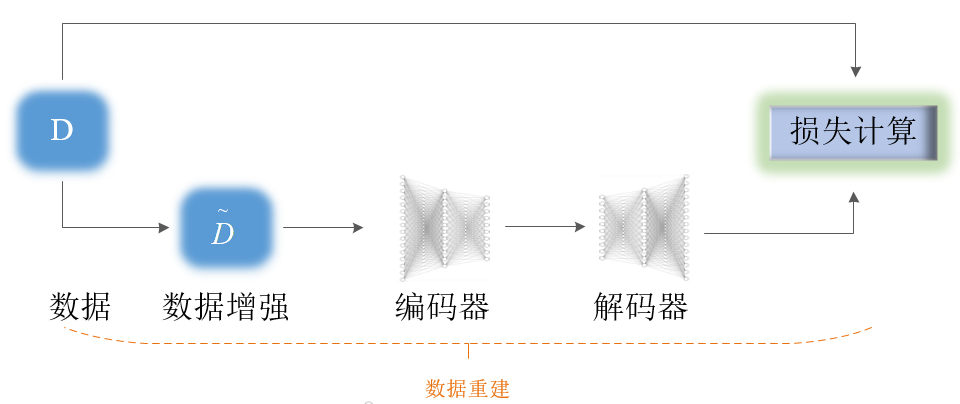
\includegraphics[width=0.8\textwidth]{self2.png}
	\caption{典型的生成型推荐算法示意图}
	\label{2Fig:self2}
\end{figure*}
%*******************************
生成型的推荐算法旨在通过使用扰动后的数据输入来重建原始输入,从而编码数据中的内在相关性。典型的生成型推荐算法如图~\ref{2Fig:self2}所示。根据它们的重建目标,可以将这些推荐算法分为两类:结构生成(Structure Generation)和特征生成(Feature Generation)。
\subsubsection{结构生成}
结构生成利用结构信息来监督模型,通过将基于屏蔽、随机丢点、随机丢边的增强操作应用于原始输入数据,可以得到其数据增强,然后训练模型对输入数据本身进行重建。例如,BERT4Rec\cite{sun2019bert4rec}通过将序列中的物品随机屏蔽,用特殊标记[mask]替换,然后重建交互下序列。最近的研究 \cite{geng2022recommendation,zhang:sigir} 迈出了探索提示学习和个性化结合的第一步。它将所有的推荐数据转换为自然语言序列,并在预训练期间使用掩码语言模型进预训练,并应用于推荐任务。
\subsubsection{特征生成}
特征生成利用特征信息来监督模型,通过在增强数据上学到的特征表示对原始特征表示进行重建。特征生成问题可以描述为一个回归问题,通常使用均方误差MSE描述重建特征表示和原始特征表示的距离。典型的方法如PMGT\cite{liu2021pre}。该方法使用提取的图像和文本特征初始化物品特征,并对采样节点的一部分进行屏蔽,然后训练基于Transformer的推荐模型,以重建恢复屏蔽节点的特征。对于序列特征生成,Ma等人\cite{ma2020disentangled}提出使用过去的行为来重建未来序列的特征表示。具体而言,将给定行为序列背后的意图进行分解,并在涉及共享意图的子序列之间进行重建。

生成型自监督推荐通常遵循掩码语言模型的流程,并依靠Transformer的强大能力取得较好的效果。特别最新的研究是将所有的推荐数据转换为自然语言序列,并在预训练期间使用语言建模目标进行预训练,但对计算资源要求较高。对于新闻推荐或通用表示的大规模数据集进行训练,则对计算资源提出了更高的要求。


\subsection{预测型推荐算法}
%*******************************
\begin{figure*}[h!]
	\centering
	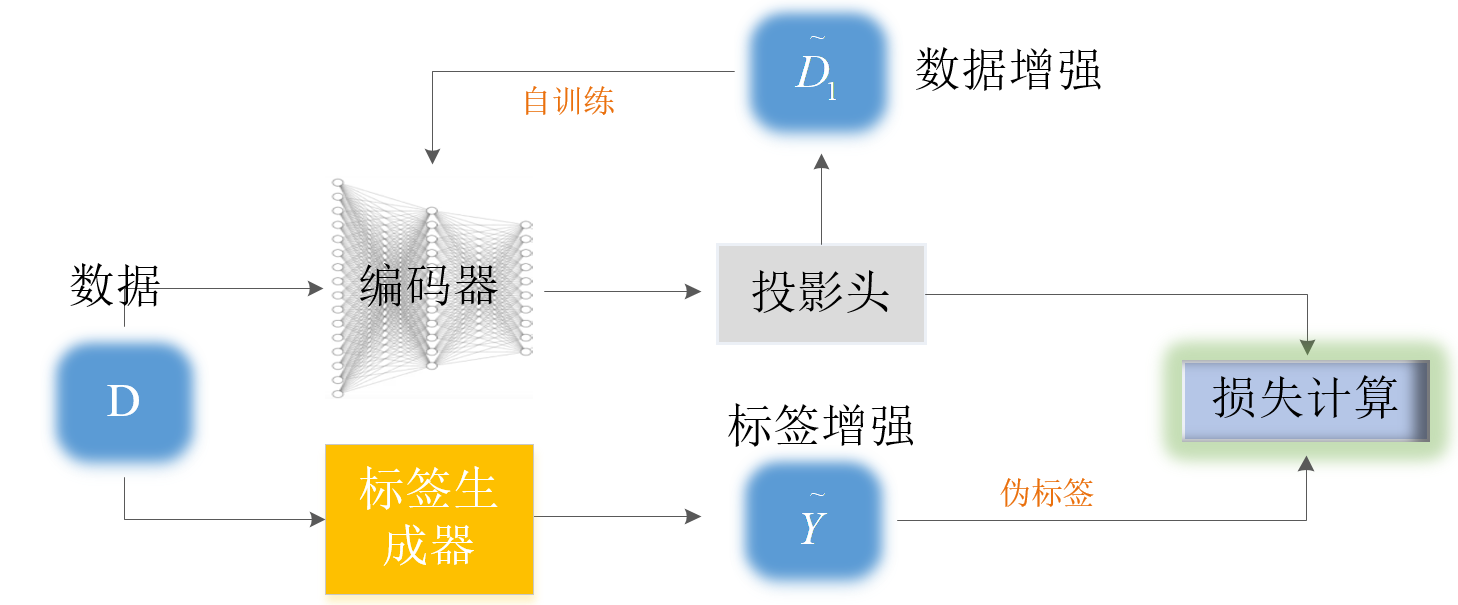
\includegraphics[width=0.8\textwidth]{self3.png}
	\caption{典型的预测型推荐算法示意图}
	\label{2Fig:self3}
\end{figure*}
%*******************************
预测型推荐算法和生成型推荐算法都涉及预测,但底层目标是不同的。生成型推荐算法侧重于预测原始数据中缺失的部分;而预测型推荐算法从原始数据中生成新的样本或标签以引导训练任务。典型的预测型推荐算法如图~\ref{2Fig:self3}所示。根据预测的任务,可以将预测型推荐分为两个分支:样本预测和伪标签预测。

\subsubsection{样本预测}
样本预测通常利用预训练模型生成的虚拟样本来监督模型,然后训练推荐模型对样本进行预测,这一方法广泛应用于序列推荐。例如,ASRep\cite{liu2021augmenting}首先以逆向方式预训练基于Transformer的编码器SASRec\cite{kang2018self},以使编码器能够生成虚拟样本。通过将虚拟的子序列添加到原始序列的开头,得到增强的序列。然后以从左到右的方式在增强的序列上进行微调,以预测原始序列中的下一个物品。例如,BiCAT\cite{jiang2021sequential}认为逆向增强可能与原始相关性不一致,于是提出同时从左到右和从右到左的方向预训练编码器,这种双向训练可以弥合逆向增强和正向推荐之间的语义差异。

\subsubsection{标签预测}
标签预测利用虚拟标签来监督模型,通过预训练的模型生成虚拟标签,然后训练推荐模型对虚拟标签进行预测。根据预测的标签形式,这些预测任务可以被形式化为关系预测和相似性预测。对于离散型标签,描述的通常是两个对象之间的关系,相应的预测任务是预测该关系是否存在。此类离散型的虚拟标签的预测任务可以被形式化为一个分类问题。例如,PTUM\cite{wu2020ptum}受BERT中的下一句预测(NSP)\cite{Devlin:2018:bert}启发,提出了预测两个序列之间的关系。该方法首先将用户行为序列分为两个不重叠的子序列,然后根据过去的交互序列预测候选物品是否为未来的交互序列。对于连续性标签的相似度预测任务,代表性的方法是BUIR\cite{lee2021bootstrapping}。该方法受到视觉模型BYOL\cite{BYOL:2020:NIPS}启发,采用了两个不对称的编码器(一个在线网络和一个目标网络)相互监督,其中目标网络生成了一个虚拟的相似度标签,用于监督在线网络的训练。

由于预测型推荐算法以动态的方式获取样本和伪标签,它们会随着模型参数不断演化,这样可以改进自监督信号,从而可能提高推荐性能。然而,大多数预测型推荐算法使用启发式方法获取伪标签,伪标签的可靠性、合理性以及与推荐任务的相关性尚缺乏评估。

%\subsection{混合型推荐算法}
%%*******************************
%\begin{figure*}[h!]
%	\centering
%	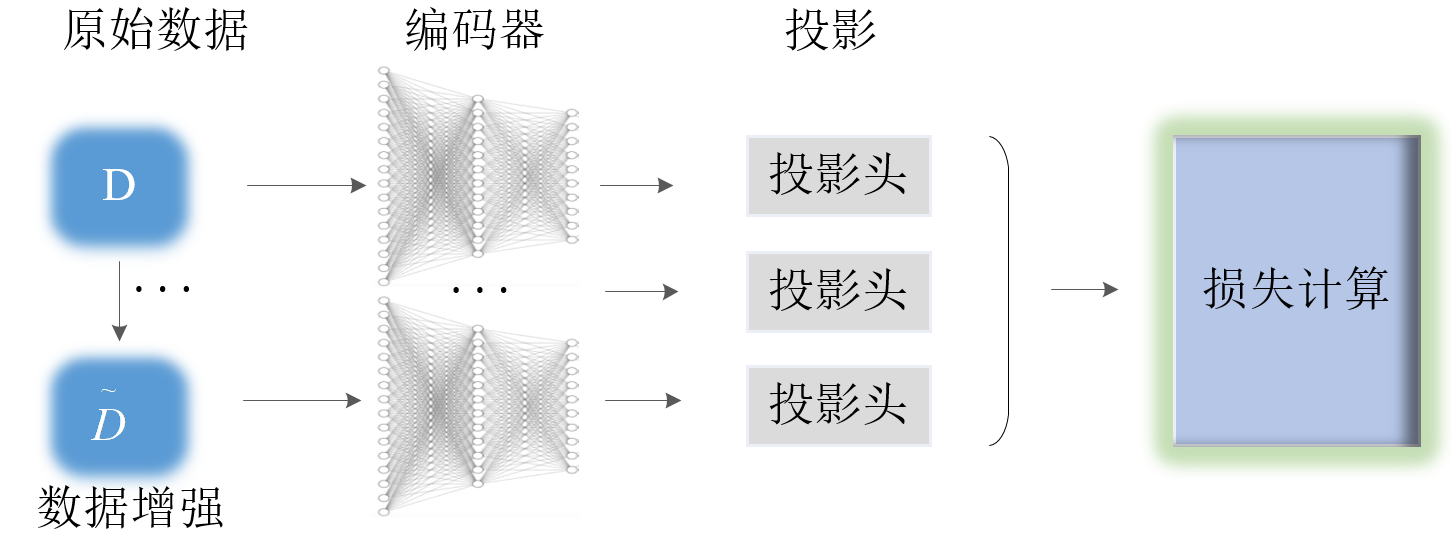
\includegraphics[width=0.9\textwidth]{self4.png}
%	\caption{典型的混合型推荐算法示意图}
%	\label{2Fig:self4}
%\end{figure*}
%%*******************************
比型推荐算法、生成型推荐算法和预测型推荐算法是自监督推荐的三种主要形式。混合方法\cite{bian2021contrastive,wang2023curriculum}利用不同的自监督信号,并组合多种类型的预训练任务,获得了增强和全面的自监督信号,在训练效果上比单一的自监督信号具有优势。然而,混合方法面临着协调多个自监督任务的问题,通常需要手动搜索超参数,以平衡不同的自监督任务。

%\textbf{协同自监督}使用多个自监督任务协同工作,以获取更全面的自监督信号。以CCL\cite{bian2021contrastive}为例,该方法提出了一种基于Transformer模型的预训练策略,将生成性预训练任务与对比性预训练任务进行组合。其中,生成性任务涉及到掩码物品的预测,预测的概率被用来增强序列,然后与原始序列进行对比。\textbf{并行自监督}方法的不同之处在于,多个自监督任务之间没有相关性,它们并行工作。以CHEST\cite{wang2023curriculum}为例,该模型组合了生成性和对比性任务。CHEST通过随机游走形成特定交互的子图。一方面,利用局部上下文信息在生成性任务中预测子图中的掩码节点/边。另一方面,利用全局相关性在对比任务中拉近原始子图和增强子图来学习子图级别的语义。

\section{对比学习相关工作}
对比学习在计算机视觉、自然语言处理等诸多领域取得了瞩目的成就,也是自监督推荐的主要实现形式\cite{SSR:2023:TKDE}。正样本、负样本以及对比损失是对比学习的核心组件,也是提升推荐性能的关键。本节首先介绍对比学习的概念,着重梳理推荐算法中广泛使用的BPR损失与InfoNCE的联系;然后梳理对比学习的相关工作,包括正样本增强、负样本采样、对比损失函数设计。
\subsection{对比学习基础概念}
从统计学习的角度来看,机器学习模型可以分为两类:生成模型和判别模型\cite{li:2019}。给定特征$X$和标签$Y$的联合分布$P(X,Y)$,生成模型旨在建模
\[p(X|Y=y)= \frac{p(X,Y)}{p(Y=y)}\]
而判别式模型旨在建模
\[p(Y|X=x)= \frac{p(X,Y)}{p(X=x)}\]
生成式模型需要重构特征$X$的像素级信息,从而捕捉特征之间的潜在关系。而判别式则是直接对后验概率建模,旨在激励编码器编码不同类别样本之间的差异特征,不编码像素级特征。对比学习属于判别式的一种,旨在通过噪声对比估计(Noise Contrastive Estimation, NCE)\cite{Gutmann:2010:ICAIS}的目标函数在比较中学习(Learn-to-Compare)
\begin{eqnarray}
\mathcal{L}_\textsc{Nce} = \mathbb E[-\log \frac{\exp(f(x)^Tf(x^+))}{\exp(f(x)^Tf(x^+))+\exp(f(x)^Tf(x^-))}]
\end{eqnarray}
其中,$x$是锚点,在推荐中通常选择用户$u$,$x^+$是锚点的正例,在推荐中通常选择为已交互的物品$i$;$x^-$为锚点的负例,在推荐中通常选择为未交互的物品$j$。$f$是编码器,$f(x)^Tf(x^+)$是由编码器参数化的正例对相似度预测得分,通常为内积相似度或者余弦相似度,记为$\hat{x}_{ui}$。类似地,$f(x)^Tf(x^-)$是负例对相似度预测得分,记为$\hat{x}_{uj}$。可以看到,NCE损失函数与BPR损失\cite{Steffen:2009:UAI}的联系:
\begin{eqnarray}
	\mathcal{L}_\textsc{Nce} 
	&=& \mathbb E[-\log\frac{\exp(\hat{x}_{ui})}{\exp(\hat{x}_{ui})+\exp(\hat{x}_{uj})}]\nonumber \\
	&=& \mathbb E[-\log\frac{1}{1+\exp(\hat{x}_{uj}-\hat{x}_{ui})}]\nonumber \\
	&=& \mathbb E[-\log \sigma (\hat{x}_{ui} - \hat{x}_{uj})]\nonumber \\
	&=& \mathcal{L}_\textsc{Bpr} 
\end{eqnarray}
其中$\sigma(\cdot)$为sigmoid函数。在实践中,由于要引入正则化项避免过拟合,而正则化项又等价于高斯分布先验密度的对数,从而BPR将上式解释为观测到的有序对的最大后验估计。尽管BPR和NCE有着不同的解释,但是BPR与NCE有着完全相同的数学形式,共享相同的优化目标。

需要说明的是,正例或者负例的语义是由自监督信号确定的。例如SimCLR\cite{Chen:2020:ICML}所使用的自监督信号是“图像增强的语义不变性”,从而把原图的增强定义为正例;BPR\cite{Steffen:2009:UAI}的自监督信号是“用户对已交互物品的偏好强于未交互物品”,从而将已交互物品定义为正例;LightGCL\cite{lightgcl:2023:ICLR}的自监督信号是“用户物品二分图(Graph)轻微扰动的语义不变性”,从而将相同的节点定义为正例。总而言之,具体的正例或负例语义由自监督信号决定,可以根据任务以及场景进行迁移和拓展。将NCE中加入更多的负例,那么可以得到InfoNCE损失\cite{Oord:2018:arxiv}:
\begin{eqnarray}
	\mathcal{L}_\textsc{InfoNCE} = \mathbb E[-\log \frac{\exp(f(u)^Tf(i))}{\exp(f(u)^Tf(i))+\sum_{n=1}^{N}\exp(f(u)^Tf(j_n))}]
\end{eqnarray}

可以看到,\textbf{NCE和BPR都是InfoNCE损失负例个数$N=1$的特例}。以最具一般性的InfoNCE损失为例,它的含义是正确分类正样本的交叉熵\cite{Oord:2018:arxiv},最小的InfoNCE损失为0,在正例相似度得分与负例相似度得分满足$f(u)^Tf(i)- f(u)^Tf(j_n)\rightarrow +\infty, n \in \{1,2,\cdots N\}$时取到。这一结论也适用于NCE和BPR,只是负例个数$N=1$。

进一步地,相似度分数与欧氏距离是一一对应的负相关关系。对于投影到单位超球面的两个$d$维向量$f(u) = (u_1,u_2,\cdots,u_d)$和$f(i) = (i_1,i_2,\cdots,i_d)$欧式距离$d(f(u),f(i))$与内积相似度分数$f(u)^Tf(i)$存在如下关系:
\begin{eqnarray}
d(f(u),f(i)) &=& \sqrt{(u_1-i_1)^2+\cdots +(u_d-i_d)^2} \nonumber \\
&=&\sqrt{2-2f(u)^Tf(i)} \nonumber
\end{eqnarray}
因此相似度分数越高,距离越近。成对损失或者对比损失与常用的均方误差损失具有明显的区别:均方误差损失是基于样本和监督标签计算得到;而成对损失或者对比损失是基于多个样本的特征表示计算得到,不涉及显式的监督标签。

基于上述分析,可以从三个方面归纳对比学习的特征:
\begin{enumerate}
\item 从数值角度看,对比学习优化正例得分大于负例得分,只优化相似度分数的差值,不优化具体值,以激励学习数据的内在结构和特性。
\item 从嵌入空间看,对比损失激励编码器拉近正例与锚点的距离,推远负例与锚点的距离,实现编码不同样本的差异特征,而非样本本身的像素级信息。文献\cite{Wang:2022:KDD}和文献\cite{Wang:2020:ICML}分别阐释了优化BPR损失以及InfoNCE损失都是渐进地优化正样本一致性(Alignment)、负样本的均匀性(Uniformity)\footnote{其中一致性要求正样本尽量接近,均匀性要求两个随机样本尽量分散。}。
\item 从统计角度看,对比学习优化“正确分类正样本的概率”\cite{Oord:2018:arxiv},体现判别式方法的特征,即直接对样本所属类别的后验概率建模。
\end{enumerate}

%\section{对比学习相关工作}
%对比学习有几个关键组件:(1)负例,(2)正例,(3)网络架构,(4)对比损失函数,共同决定了对比学习的效果。本节根据对比学习的组件,分别从负例采样方法、正例增强方法、网络架构设计和损失函数设计四个方面总结对比学习的相关工作。
\subsection{负样本采样方法相关工作}
%*******************************
\begin{figure*}[!]
	\centering
	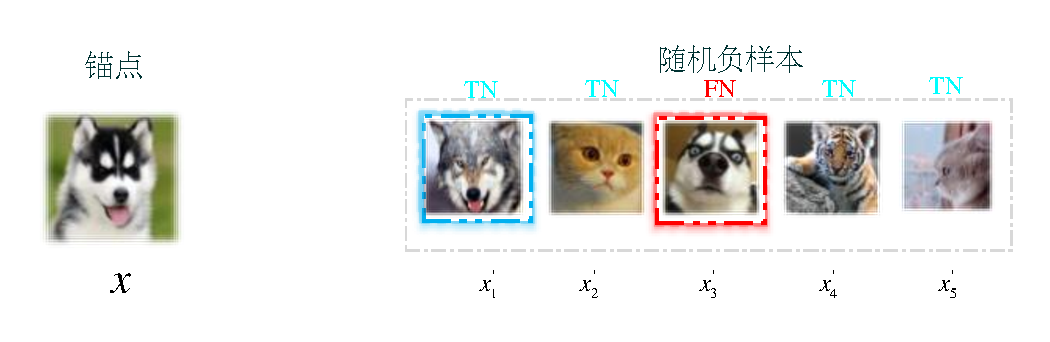
\includegraphics[width=0.9\textwidth]{fhn.pdf}
	\caption{困难负例和伪负例示意图}
	\label{2Fig:illustrative}
\end{figure*}
%*******************************
对比学习有两个关键目标,拉近正样本并推远负样本。如果仅仅拉近正样本,即只最小化正样本之间的距离,可能会使得神经网络学到坍缩的解,即为所有的样本输出相同的表示。因此,推远负样本也必不可少。但是在大多数情况下缺乏明确的负信号,因此从未标注样本中采样负例的负采样策略被广泛研究。以图\ref{2Fig:illustrative}的一个直观的示例解释负采样策略的两个关键目标:锚点为狗,样本$x_1^\prime$是狼,与锚点不同类,但是特征很相似,称为困难负样本(Hard Negative Sample)。样本$x_3^\prime$是狗,与锚点同类,由于缺乏监督标签也出现在负例候选集,称为伪负样本(False Negative Sample)。为了使得同类样本的表示距离较近,那么$x_1^\prime$狼这个困难负例应该被选作负样本,使其被推远,防止其混入狗这个类别;且$x_3^\prime$狗这个伪负例不应该被选作负样本,防止其被推远。推荐领域的任务也是一样,只是正负样本语义是喜欢与否。负采样(NS)的策略是从候选的未标注样本中采样负样本,核心目标围绕如何采样困难负样本且剔除伪负样本展开。许多研究表明,负采样对于提高下游的分类或推荐性能非常重要~\cite{Steffen:2014:WSDM,Zhang:2013:SIGIR,Ding:2020:NIPS,Park:2019:WWW,Huang:2021:KDD,Ding:2019:IJCAI,Yang:2020:KDD}。

\subsubsection{采样困难负样本}
采样困难负样本的主要目标是采样类似于样本$x_1^\prime$这样的困难负样本。它们与正例很相似,但是所属类别为负类。由于这两个样本在特征上相似度很高, 难以区分,在经过网络提取特征之后, 它们特征之间的相似度分数也比较高。采样此类样本一方面会使得不同类别的困难负样本被推远,迫使神经网络学习难以区分的样本之间的边界;另一方面,这类样本与锚点的相似度分数较高,梯度值较大,从而神经网络的参数更新更多,提高模型训练效率。基于上述动机,很多困难负采样(Hard Negative Sampling)方法被提出,这类方法普遍采用随模型训练动态调整的采样分布,以针对困难负例进行采样~\cite{Steffen:2014:WSDM,Zhang:2013:SIGIR,Ding:2020:NIPS,Park:2019:WWW,Huang:2021:KDD,Ding:2019:IJCAI}。

在推荐领域,困难负采样实现的典型思路是采样相似度分数较高,或排序位置靠前的样本。最具代表性的困难负采样方法为动态负采样\cite{Zhang:2013:SIGIR}。动态负采样通过在若干个候选的负例中采样相似度分数比较高的样本,从而实现每个样本的采样概率正比于其相对排序位置。类似地,Steffen等人\cite{Steffen:2014:WSDM}提出针对排名位置靠前的样本进行采样。这两个经典思想是类似的,因为排序位置与相似度分数是一一对应的。除了使用分数相似度或者相对排序位置来表征样本的困难等级(Hardness Level),还有研究者使用图的相关信息来采样困难负样本。例如,Wang等人~\cite{Wang:2020:WWW}和Wang等人~\cite{Wang:2021:CIKM}提出利用知识图谱上的关系类型来采样困难负例。另一种方使用较多的是选择与正例在图结构上相似的困难样本~\cite{Chen:2019:WWW,Wang:2021:TKDE,Ying:2018:KDD}。文献\cite{shi2023theories}分析了,困难负采样实际上是在优化推荐列表指定伪正例例率(FPR)范围内的AUC面积(One-way Partial AUC, OPAUC),但没有考虑伪负例问题。

\subsubsection{剔除伪负样本}
剔除伪负样本的主要目标是避免采样类似于样本$x_3^\prime$这样与锚点同类的样本。由于缺乏标签,它们虽然出现在负例候选集,但是所属类别为正类。在推荐领域,这类样本对应于用户没有看到过,但是潜在喜欢的物品。由于这个样本所属类别为正类,因此应当避免采样到此类样本,防止其在嵌入空间被推远。另一方面,采样此类物品,会使得模型误判用户的兴趣边界。因此,负采样的另外一个重要目标就是防止采样到伪负例。最普遍方法是使用附加信息来避免采样伪负例。这些附加信息对于提取负信号非常直观,例如社交网络中用户的连接关系~\cite{Zhao:2014:CIKM,Wang:2016:CIKM}、用户的地理位置~\cite{Yuan:2016:IJCAI,Liu:2019:IJCAI},以及额外的交互数据,如已查看但未点击的数据~\cite{Jingtao:2019:IJCAI, Jingtao:2018:WWW},但是这些额外信息通常不好获得,只有特定的数据集才有。

为了避免采样伪负例,还有一类新的方法是使用多个未标记样本中生成虚拟的负样本用于模型训练。例如,Huang等人~\cite{Huang:2021:KDD}提出通过混合候选负样本的嵌入来合成虚拟的困难负例。Jun等人~\cite{Jun:2017:SIGIR}和Park等人~\cite{Park:2019:WWW}设计了生成对抗神经网络来生成虚拟的困难负例。合成虚拟负样本的方法也广泛使用在计算机视觉中,例如Zhu等人\cite{zhu:2021:iccv}提出了在特征空间上将负样本对应的嵌入插值,类似于构造了虚拟的负样本,而对正样本的嵌入外推,最终提高了对比学习的效果。 Zhong 等\cite{zhong:2021:cvpr}提出了一种结合图像混合 (Mixup) 技术的困难样本构造方法, 首先使用Mixup合成虚拟的负样本,然后依据合成负样本的相似度分数选择困难的合成负样本进行对比学习训练。

总体来说,负采样方法取得较大进展,特别是困难负采样方法对于下游任务性能提升效果非常显著。采样困难样本是容易实现的,只需要采样相似度分数高或者距离近的样本。但是如何从困难样本中采样真负例,还是严重依赖额外信息作为监督信号。尽管合成虚拟负样本的方法看似避免了采样伪负例,但是它的实质是将更多的样本包含在对比损失的分母中:虚拟样本嵌入是若干个负例的混合,那么虚拟样本的相似度分数是这几个负例相似度分数的函数,更多的样本用于合成虚拟样本,导致更多的样本包含在对比损失的分母中,并没有从根本上解决伪负样本问题。
\subsection{正样本数据增强相关工作}
正样本数据增强的目标是获取语义不变的正样本用于对比。数据增强是获取语义不变的正样本的主要途径,也是提升自监督信号的重要来源。在计算机视觉中,通常的做法是通过在锚点$x$上进行某些语义不变的数据增强来获得正样本$x^+$,如随机裁剪和翻转\cite{Oord:2018:arxiv},图像旋转\cite{Komodakis:2018:ICLR},和颜色失真\cite{Szegedy:2015:CVPR}等。然而,仅采用单一的图像增强方法并不利于性能提升,SimCLR\cite{Chen:2020:ICML}方法综合比较了一系列图像变换方法的效果,并发现将随机裁剪和颜色失真组合起来的变换方式能够获得更好的效果。

受到图像领域的启发,在推荐领域的数据增强工作也得到了广泛的研究。然而,推荐系统数据集通常以用户物品二分图的形式存在,节点只包含ID,往往使用基于图的策略进行增强。在推荐中数据增强的核心思想是在原有用户二分图结构的基础上略作扰动。这种增强的用户物品二分图被认为保留了结构信息,相同ID的节点即为正样本。图数据的增强策略可以分为以下几种(1)基于特征的增强\cite{liu2022local,velivckovic2018deep,zhu2020deep,you2020graph,pmlr-v139-you21a}:仅对节点或者边的特征矩阵进行变换。通常随机屏蔽节点或边属性的一小部分,并用常数或随机值替换。(2)基于结构的增强\cite{pmlr-v119-zheng20d,10.1145/3437963.3441734,10.1145/3437963.3441720,page1998pagerank}:仅对邻接矩阵进行变换。通常随机(或手动)在图中添加或删除一小部分边,包括边扰动\cite{pmlr-v119-zheng20d,10.1145/3437963.3441734}、节点插入\cite{10.1145/3437963.3441720}和边扩散\cite{page1998pagerank}、图采样\cite{pmlr-v119-zheng20d}等方法。

%(3)基于标签的增强\cite{Steffen:2014:WSDM,zhang2020graph,verma2019manifold}:由于图上人工标注标签的不足,通过标签增强用于增加有限的标记训练数据。它可以分为两类:一类是伪标签的增强,例如PTUM\cite{wu2020ptum}将用户行为序列分为两个不重叠的子序列,构建了两个序列之间的关系的标签。第二类是数据混合\cite{zhang2020graph,verma2019manifold},直接插值构建虚拟的负样本。VGCL\cite{yang2023generative}综合考虑了特征增强和结构增强的缺陷,利用变分图重构来估计每个节点的高斯分布,然后从估计分布中进行多个采样来,生成多个对比视图。LightGCL\cite{lightgcl:2023:ICLR}则将归一化的邻接矩阵进行奇异值分解,通过抛弃被认为是噪声的较小奇异值,获得了增强视角的图用于对比。

总体来说,由于图数据具有固有的非欧几里得特性,很难将图像中的随机剪裁、反转、颜色失真等保持语义不变的数据增强方法应用于图数据。基于随机过程的图数据增强可能会损失图中重要的结构信息,因为随机丢弃的点或者边可能会体现图的重要结构信息。此外,图增强对于推荐任务的有效性存在一些质疑\cite{yu2022graph},有待更深入和更系统地调查。

%
%\subsection{网络架构设计的相关工作}
%既然数据增强对于提升自监督对比学习的效果至关重要,那如设计更有效的网络架构,从而享受更密集的数据增强带来的好处?此外,负例的未标注是自监督对比学习与有监督对比学习的主要差异。既然有限的监督信号下难以避免采样伪负例。那么是否可以不用负样本,同时避免神经网络学到坍缩解?基上述两个主要动机,不同的网络架构被提出。由于相似度分数$\exp(f(x_1)^T,f(x_2))$计算涉及两次对样本的编码,下文把编码第一个样本的网络称为网络分支1,把编码第二个样本的网络称为网络分支2。根据两个网络分支的架构是否相同,可以分为同构网络和异构网络:前者网络分支架构相同,后者网络分支架构不同;根据两个网络分支参数的更新方式是否相同,可以分为同步网络和异步网络:前者通常采用端到端的反向传播方式更新网络参数,后者的网络分支更新方式不同,往往分别使用梯度法和动量法分别跟新两个网络分支参数。
%\subsubsection{同步同构网络架构}
%典型的同步同构网络如图\ref{2Fig:arc1}所示,代表性工作是SimCLR\cite{Chen:2020:ICML}。它采取了最自然的端到端地反向传播的方式更新神经网络参数,且两个网络分支的架构完全相同。给定一个样本,经过两次增广获得正样本对,从而受益于更密集的数据增强;然后, 通过同一个神经网络模型将样本投影到嵌入空间。这里,同一个神经网络模型即可以看作两个同构的网络分支。 对同一个Mini Batch的$N$个数据进行同样操作后,得到$2N$个表示向量;然后, 根据这$2N$个表示向量经过多层感知机(MLP)非线性映射得到投影;最后,根据投影计算InfoNCE损失,然后反向传播更新梯度。由于它使用一个神经网络模型,可以看作两个完全相同的网络分支,因此是同构网络;此外,两个网络分支是端到端地进行反向传播更新参数,因此是同步网络。
%%*******************************
%\begin{figure*}[h!]
%	\centering
%	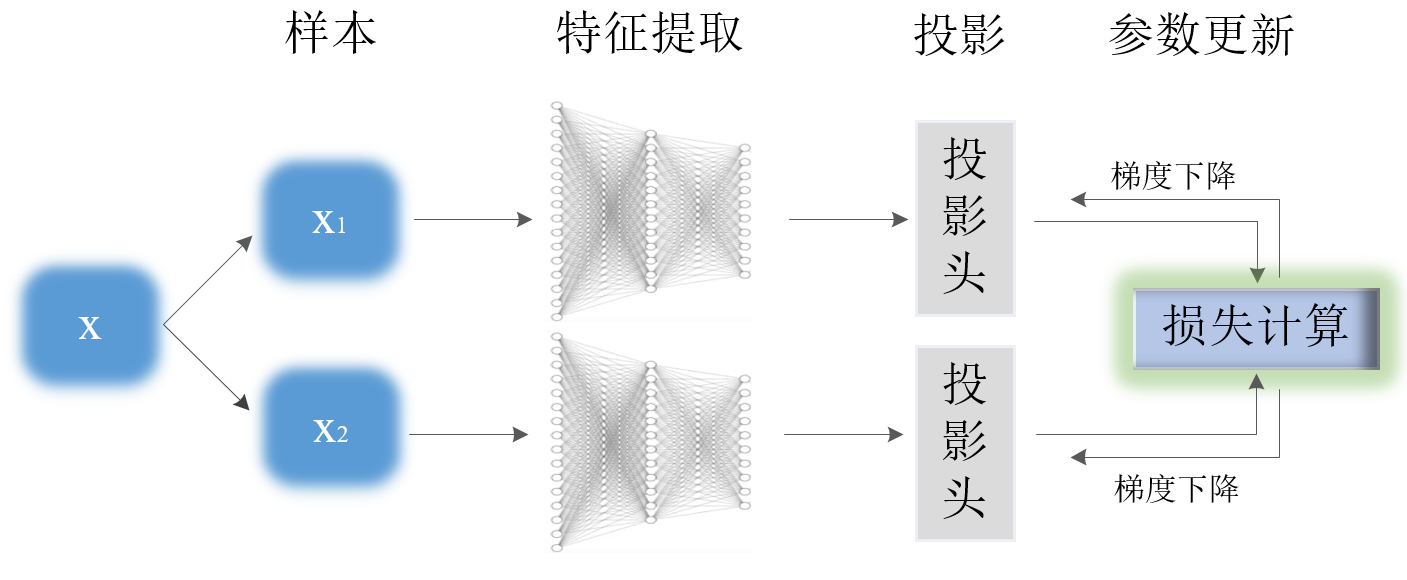
\includegraphics[width=0.8\textwidth]{arc1.png}
%	\caption{同步同构网络架构示意图}
%	\label{2Fig:arc1}
%\end{figure*}
%%*******************************
%
%在推荐中的网络架构大都可以归纳为同步同构网络架构,但工作机制略有不同。以最常用的LightGCN\cite{Xiangnan:2020:SIGIR}为代表,第一个网络分支编码用户表示,第二个网络分支编码物品表示,即双塔结构。聚合后的用户物品表示无需投影,直接计算损失,然后反向传播更新用户和物品表示。由于用户物品表示都是采用梯度更新的方式,因此是同步更新方式;此外用于聚合用户和物品的图卷积神经网络结构相同,因此是同构网络。另一种具有代表性的是LightGCL\cite{lightgcl:2023:ICLR}:第一个网络分支编码原图的用户表示,第二个网络分支依旧编码增强图的用户表示。LightGCN优化用户和喜欢的物品表示尽量相似,和不喜欢的物品表示尽量不相似;LightGCL则优化不同视图下同一个用户的表示尽量相同,与其他用户表示尽量不同,物品表示同理。这种差异主要是源自于对正负样本的定义和语义不同:LightGCN中用户和喜欢的物品构成正样本对,LightGCL中不同视图下的同一用户构成正样本对,同一物品也构成正样本对。这是正例对(或者负例对)的定义和语义不同,不影响网络架构的组织形式以及参数更新方式。
%\subsubsection{同步异构网络架构}
%%*******************************
%\begin{figure*}[h!]
%	\centering
%	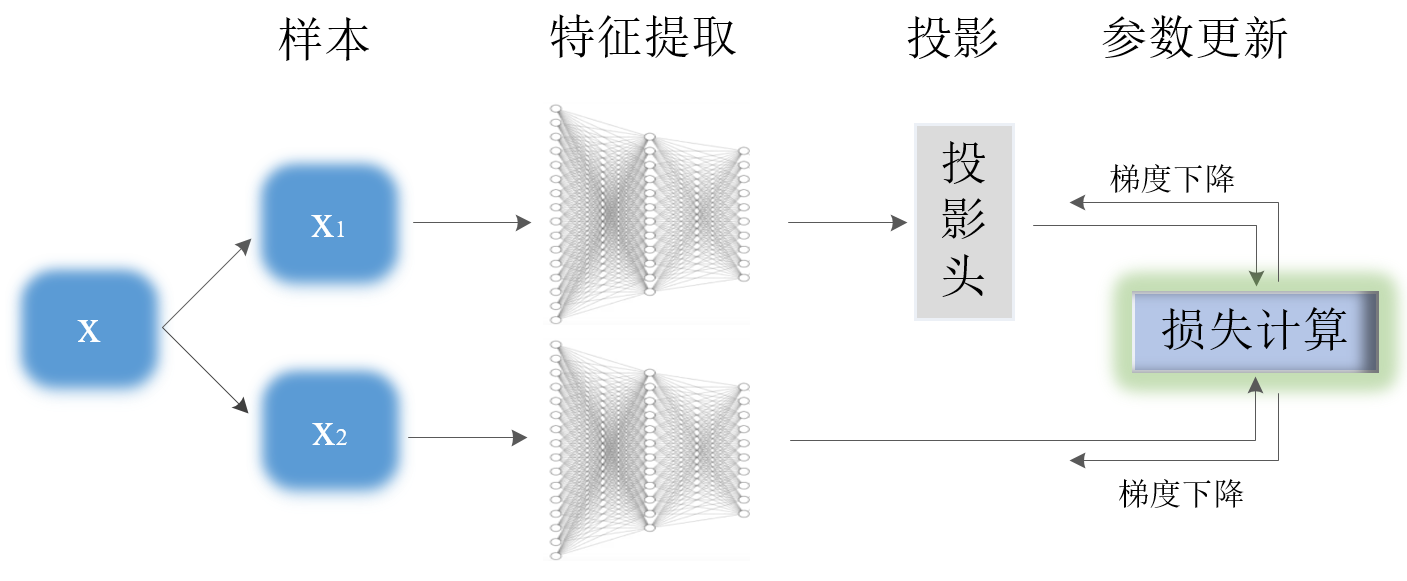
\includegraphics[width=0.8\textwidth]{arc2.png}
%	\caption{同步异构网络架构示意图}
%	\label{2Fig:arc2}
%\end{figure*}
%%*******************************
%典型的同步异构网络如图\ref{2Fig:arc2}所示:两个网络分支的参数更新方式是相同的,都采用梯度下降更新参数;但网络分支的架构不同,两个网络分支采用不同的网络结构。网络结构的不同主要有三种:(1)分支1包含投影头,分支2不包含投影头\cite{Oord:2018:arxiv}。(2)分支1和分支2都含有投影头,但投影头的结构不相同\cite{misra:2020:CVPR}。(3)用于特征提的分支1和分支2的网络结构不相同\cite{chaitanya:2020:NIPS}。以第一种为例,介绍同步异构网络架构的工作机制,典型的工作是对比预测编码(contrastive predictive coding, CPC)。在该方法中,分支1接收某个时间点的数据作为输入,分支2接收未来某个时间点的数据作为输入,目标是利用分支1的输出来预测分支2的输出,以最大化已知数据和待预测数据的互信息。在计算损失后,两个网络分支均按梯度法更新参数。
%\subsubsection{异步同构网络架构}
%%*******************************
%\begin{figure*}[h!]
%	\centering
%	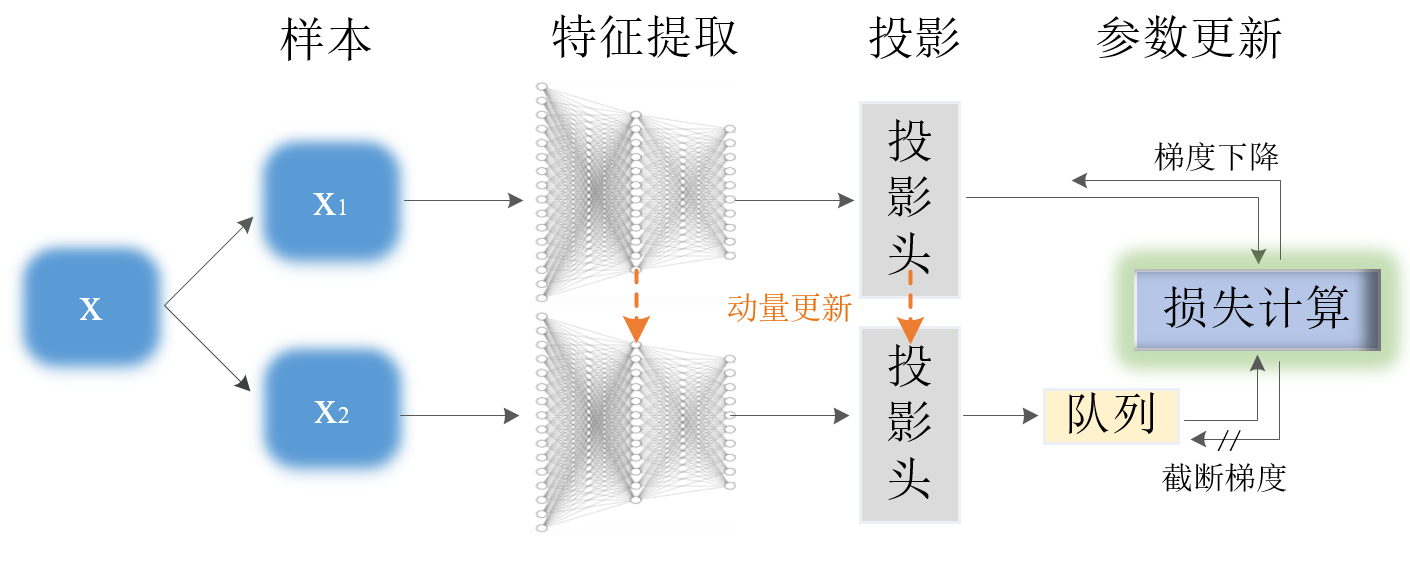
\includegraphics[width=0.8\textwidth]{arc3.png}
%	\caption{异步同构网络架构示意图}
%	\label{2Fig:arc3}
%\end{figure*}
%%*******************************
%典型的异步同构网络架构如图\ref{2Fig:arc3}所示:两个网络分支架构相同,但参数更新方式不同:网络分支1采用梯度下降更新参数,而网络分支二采用动量法更新参数。使用这种异步同构的网络架构典型工作是MoCo\cite{He:2020:CVPR}。网络分支1和网络分支2架构完全相同,初始化参数也相同。第一个网络分支按照正常操作获得样本投影的特征,但是第二个网络分支把投影的特征压入队列,直到队列达到指定长度以后,对最先入队的样本特征执行出队操作,从而获得一个较大的负样本数量。最后,根据正样本的投影特征计算损失。回传梯度时,只有第一个网络分支执行反向传播更新参数,第二个网络分支的参数根据第一个网络学到的参数进行动量更新。记第一个网络分支的参数为$\theta$,第二个网络分支的参数为$\xi$,那么它们的更新方式可以写为:
%\begin{eqnarray}
%	\theta &\leftarrow& \text{optimizer}(\theta,\nabla_\theta \mathcal{L}) \nonumber\\
%	\xi &\leftarrow& \tau \xi + (1-\tau)\theta \nonumber
%\end{eqnarray}
%其中第一个网络分支的参数$\theta$通过梯度法更新以后,将学到的最新的参数$\theta$,取$(1-\tau)\theta$用于更新第二个网络分支的参数。可以看到,只有第一个网络分支参数更新以后,才能更新第二个网络分支,因此称这种参数更新方式为异步法。当衰减系数$\tau$比较大时,第二个网络分支的参数更新幅度很小。异步法区别于端到端地使用梯度下降法更新两个网络分支,它们的更新是同步的。
%
%MoCo的第一个核心操作是对网络分支2编码得到的特征执行入队操作,解耦了负样本数量与批量大小,负样本数量不再受限于GPU显存大小,从而可以为对比学习设定一个较大的负样本数量。而较大的负样本数量会推高已知数据和待预测数据互信息的下界,从而取得更好的性能。此外,较大的负样本数量也会使得正例的梯度值增加,使得神经网络模型从正样本的数据增强中学到更多信息。MoCo的第二个核心操作是,网络分支2根据网络分支1学到的最新参数,使用动量法跟新参数而非使用梯度法更新参数,一方面可以避免伪负例产生的错误梯度的影响,另一方面避免神经网络学到坍缩的解。
%
%\subsubsection{异步异构网络架构}
%
%典型的异步异构网络架构如图\ref{2Fig:arc4}所示:两个网络分支架构不同,参数更新方式也不同,代表性工作是BYOL\cite{BYOL:2020:NIPS}。在参数更新方式上,网络分支1(在线网络)采用梯度下降更新参数,而网络分支2(目标网络)采用动量法更新参数。在网络结构设计上,两个网络分支采用MoCo作为主干网络,但投影头的数量不一致,网络分支1增加了一个预测头,以提高灵活性。在损失计算上,与先前的工作截然不同:之前的工作都涉及到同一批次内的其它样本作为负样本以计算对比损失,但是BYOL的计算只涉及一个样本的两个增强视角的特征投影,只约束正例对提取到的特征尽量相似。相当于完全抛弃了负例,只优化正例的对齐,不优化负例均匀,同时实现避免了神经网络学到了坍缩解。
%%*******************************
%\begin{figure*}[h!]
%	\centering
%	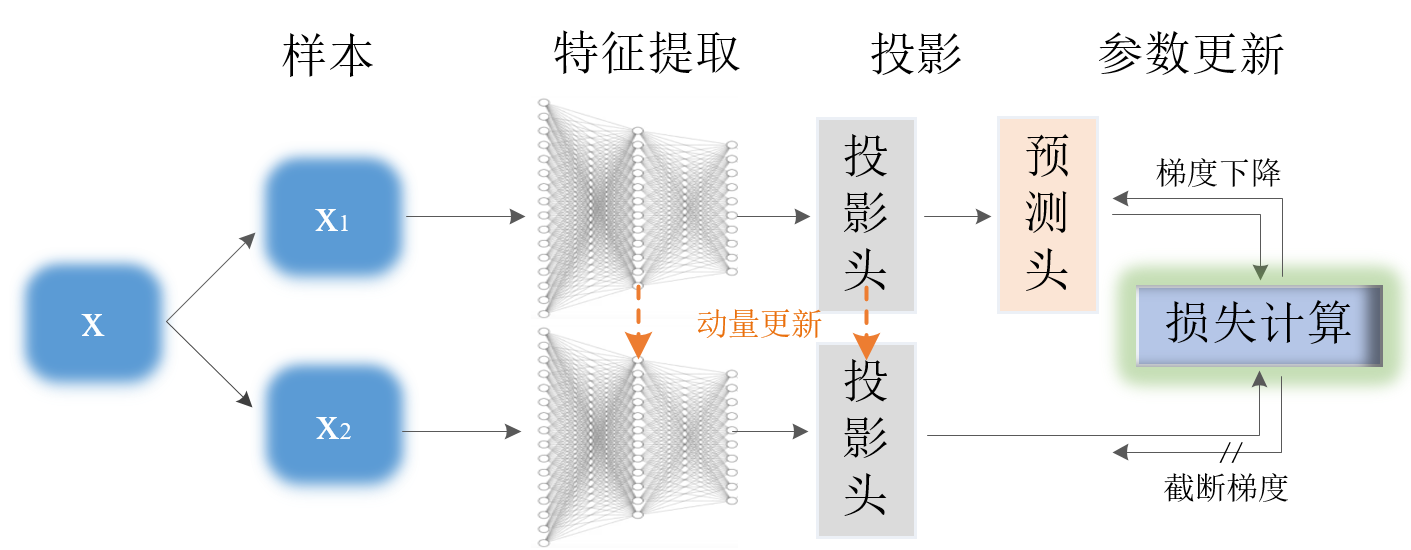
\includegraphics[width=0.8\textwidth]{arc4.png}
%	\caption{异步异构网络架构示意图}
%	\label{2Fig:arc4}
%\end{figure*}
%%*******************************
%
%BYOL的第一个核心操作是和MOCO一样,在线网络分支使用梯度法更新参数,第目标网络分支采用动量法更新参数。动量法更新也称指数滑动平均法(exponential moving average,EMA),尤其是在其衰减系数$\tau$比较大时,目标网络的参数更新很慢。第二个核心操作是给在线网络加了一个经过归一化的预测头,且其参数不会更新给目标网络,相当于在线网络提取的特征和目标网络提取的特征存在缓冲地带。这两个操作都有助于分散特征,避免神经网络学到坍缩解。第三个核心操作是损失的计算,完全不涉及负样本,只涉及正样本对的特征。具体的,是经过L2归一化的两个正样本对特征向量的均方误差,相当于只约束正样本对特征的方向。由于BOYL只优化正例对的均匀,不优化负例的均匀,从而避免了伪负样本的错误梯度问题。

\subsection{损失函数设计的相关工作}
损失函数是实现对比学习“拉近同类正样本、推远不同类负样本”的关键,从而激励编码器编码不同类别样本之间的差异信息,而非样本的像素级信息,是对比学习的核心组件。对比损失中应用最为广泛的是InfoNCE\cite{Oord:2018:arxiv},尽管BPR\cite{Steffen:2009:UAI}、NCE\cite{Gutmann:2010:ICAIS}是InfoNCE损失负例个数为1的特例,且工作远早于InfoNCE,但是InfoNCE率先构建了对比损失优化与互信息优化之间的关联。InfoNCE也广泛应用于推荐领域的图对比任务和偏好对比任务,文献\cite{Jiancan:2022:arxiv}证明了在偏好对比任务中,优化InfoNCE损失等价于优化NCDG指标。本节以更具一般性的InfoNCE损失为主线,梳理损失函数设计的相关工作。这些针对InfoNCE的改进可以很容易类比到负例个数为1的BPR损失。
\subsubsection{面向正负样本语义拓展的损失函数改进}
为了获取更密集的数据增强,SimCLR\cite{Chen:2020:ICML}将同一个样本增强两次,那么同一个批次内的N个样本经过两次数据增强就得到了2N个样本。同一个样本的两次增强$z_i,z_j$互为正例对,构造了如下对比损失
\[
\mathcal{L} = -\log \frac{\exp(f(z_i)^Tf(z_j))}{\sum_{k=1}^{2N}\mathbb I (k \neq i)\exp(f(z_i)^Tf(z_k))}
\]
其中分子是同一个样本的两个增强视图的相似度,分母是同一个样本的两个增强视图的相似度加上与其它图像两个增强视图的相似度,合计2N-1项。可以看到与InfoNCE的数学形式是一致的,只是拓宽了正负样本对的概念。MOCO\cite{He:2020:CVPR}变化在于负样本是一个提取的特征组成的队列,损失的计算方式与InfoNCE相同。

在推荐中通过一些附属信息将正负样本对的概念进行拓展,构造了更具细粒度的正负样本对,从而提取更密集的自监督信号。例如被购买的物品比只浏览的物品更受用户喜欢\cite{Qiu:2018:IS};多次交互的物品比只有一次交互的物品更受喜欢\cite{Lerche:2014:RS};用户未看到的物品应该比曝光给用户但没有交互的物品更受喜欢\cite{Wenhui:2019:WWW,Yu:2018:CIKM,Bin:2020:IS}。这类正负样本的语义下的对比学习任务是排序导向,目标是将用户喜欢的物品排在不喜欢的物品之前,与推荐任务具有一致性;此外,LightGCL\cite{lightgcl:2023:ICLR}将不同视图下的相同节点视为正样本对,不同节点视为负样本对。这类正负样本的语义对应的对比学习任务是学习图结构信息,与推荐任务不一致,通常要与第一类学习任务联合训练。在损失函数分析中,通常不区分由于正负样本对的概念拓展造成的损失函数与原始对比损失函数的差异。

\subsubsection{面向模型坍塌问题的损失函数改进}
由于对比损失优化正例对齐,神经网络的参数空间存在一种可能的解,它为所任意样本映射为同一个相同的特征表示,这样的解也称坍缩解或者模型坍塌\cite{jing2021understanding}。尽管负例参与学习训练有助于分散特征(Scatter Feature),避免模型坍塌,但也不能完全避免这种情况。基于这种情况DirectCLR\cite{jing2021understanding}取特征向量的前d维的子向量,计算对比损失
\[
\mathcal{L} = -\log \frac{\exp(f(z_i^\prime)^Tf(z_j^\prime))}{\sum_{k=1}^{2N}\mathbb I (k \neq i)\exp(f(z_i^\prime)^Tf(z_k^\prime))}
\]
其中,$z^\prime = z[0:d]$是原始特征向量的前d个维度构成子向量,这个对比损失与SimCLR损失的唯一区别就是只取每个特征向量的前d维。

BYOL\cite{BYOL:2020:NIPS}进一步改进了对比损失。对同一个样本的两次增强,两个网络分支学到的归一化特征表示分别记为$\bar q(z)$和$\bar z\prime $,BYOL优化归一化特征表示的均方误差:
\[||\bar q(z)-\bar z\prime||^2 =2-2\cdot \frac{\langle q(z),z\prime \rangle}{||q(z)||_2\cdot||z\prime||_2  } = 2-2\cos(q(z),z\prime)\]
其中为$q(z),z\prime$分别为两个网络分支学到的特征表示向量(未归一化)。可以看到,BYOL实际上只约束两个网络分支学到的特征表示的方向一致,并不规定正例对表示向量的具体模值。除了损失函数外,BYOL还通过精致的网络架构设计和正则化技术分散特征,避免神经网络学到坍缩解。

\subsubsection{面向梯度消失问题的损失函数改进}
InfoNCE损失函数的形式决定了其正例梯度等于所有负例梯度的和,符号相反\cite{Feng:2021:CVPR}。对于一个分数较小的负样本(容易负样本),或者分数较大的正样本(容易正样本),梯度容易消失,使得模型从样本中学到较少的信息。具体到负例个数为1的BPR损失中,就有正例的梯度等于负例的梯度,同样符号相反,使得梯度消失的问题更加明显,因此往往需要通过保持较大的负例个数N,以避免梯度消失的问题\cite{He:2020:CVPR}。于是解耦对比损失\cite{yeh:2022:ECCV}(Decoupled Contrastive Learning)去掉了InfoNCE失函数分母中两个正样本对之间的相似度,损失函数的形式计算如下:
\[
\mathcal{L} = -\log \frac{\exp(f(x)^Tf(x^+))}{\sum_{i=1}^{N}\exp(f(x)^Tf(x^-))}
\]
解耦对比损失避免了负样本数量对梯度的放缩,在一定程度上解决了容易正样本和容易负样本所导致的梯度消失问题。


\subsubsection{面向优化目标偏离问题的损失函数改进}
在自监督场景下,InfoNCE损失实际上优化实例之间的对齐和均匀,而非不同类别样本的均匀与对齐。更具体地,在自监督场景下,由于未标记的样本都被视作负样本,InfoNCE实际上是拉近正例与锚点之间的距离,\textit{推远任意样本与锚点之间的距离,而非负例与锚点之间的距离}。在个性化推荐中,任意未交互(未标注)的物品都被视作负例被推远;在计算机视觉中,锚点以外的任意未标记样本都被视作负例被推远。负例的无监督,使得自监督场景下InfoNCE偏离了原始的优化目标,对下游分泛化性能产生了不利的影响。为了鼓励编码器去编码数据的语义结构,拉近同类样本,推远不同类样本,ProtoNCE\cite{Li:2021:ICLR}通过改进正负样本对的语义,以改进对比损失。具体地,当前样本的特征与其对应的聚类中心构成正样本对,而与其他聚类中心形成负样本对,从而得到如下优化目标:
\[
\mathcal{L} = -\log \frac{\exp(f(x)^Tf(c_i))}{\sum_{i=1}^{C}\exp(f(x)^Tf(c_i))}
\]
其中$c_i$为聚类中心,也被称为原型(prototypes),通过在EM算法的期望步骤中执行k-means聚类得到。通过将正样本修改为锚点所属类中心,负样本修改为其他聚类中心,实现将优化目标改进为拉近样本与所属类别中心的距离,推远样本与其它类别中心的距离。这一思想在个性化推荐中也有应用\cite{lin2022improving}。

上述方案需要迭代计算,开销较大。另外一个解决负例无监督的途径是通过校正负样本相似度分数,以获取一个与有监督对比损失一致的改进损失函数,从而取得类似于监督学习的泛化效果,代表工作是去偏对比学习\cite{Chuang:2020:NIPS}(Debiased Contrastive Learning, DCL)。其核心思想是,由于伪负例包含在InfoNCE的分母中,导致的结果是分母中的负例相似度分数计算不准确。可以通过修正负例的相似度分数,实现对有监督对比损失的近似。其损失函数计算如下
\[
\mathcal{L} = -\log \frac{\exp(f(x)^Tf(x^+))}{\exp(f(x)^Tf(x^+) + N\cdot g}
\]
其中$g$是对真负样本与锚点相似度分数期望值的估计,其具体形式在后面的章节中会有更详尽的介绍。

在去偏对比学习\cite{Chuang:2020:NIPS}的伪负例去偏的基础上,HCL\cite{Robinson:2021:ICLR}进一步地考虑了硬负例挖掘,即将困难负样本推远离锚点。它遵循DCL的框架,并通过如下方式进一步地加权未标注样本的相似度分数:
\[\omega_i^\textsc{Hcl} = \frac{\hat{x}_j^\beta}{\frac{1}{N} \sum_{j=1}^{N}\hat{x}_j^\beta}
\]
其中$\hat{x}$是未标注样本与锚点的相似度分数,$\beta$是超参数。因此,未标注样本的相似度分数越高,其分配到的权重就越大,导致其被推的越远。基于估计校正的损失函数改进,避免了额外的计算开销,取得了很好的效果。

总体来说,损失函数设计相关工作取得较大进展,特别是在原理层面,现有的研究揭示了对比学习取得良好泛化性能的关键是(1)正样本特征的一致性;(2)负样本特征分布具有均匀性\cite{Wang:2020:ICML,Arora:2019:ICML}。从一致性要求考虑,应当防止同类样本被推远;从均匀性要求考虑,应当使得不同类样本被推远。对于一个未标注样本,无法确它所属类别,使得一致性和均匀性存在矛盾。尽管现有的去偏差方法通过损失校正构建了与有监督对比损失的关联,但是自监督对比学习与有监督对比学习仍存在较大距离,一致性与均匀性困境仍是一个尚待解决的问题\cite{Feng:2021:CVPR,zhang:cl}。

\section{预备知识}
本节介绍三个本文会频繁使用的工具,分别为经验分布函数、次序统计量和极大似然估计。
对于深度神经网络而言,准确推导其输出的相似度分数的分布是很困难的,本文会频繁使用来自样本计算得到的经验分布函数来刻画总体分布特征。此外,个性化推荐是一个排序任务,因此会频繁使用到次序统计量用于排序分析。最后,成对学习是极大似然估计量,因此也会频繁使用到。


\subsection{经验分布函数}\label{ecdf}
在介绍经验分布函数之前,先回顾累积分布函数(Cumulative Distribution Function, CDF)的定义。对于一个实值随机变量$X$,累积分布函数(CDF)在x处的值表示随机变量X取值小于或等于x的概率
\[F(x) = \mathbb P (X\leq x)\]
$F(x)$满足${\displaystyle \lim _{x\rightarrow -\infty }F(x)=0}$且${\displaystyle \lim _{x\rightarrow \infty }F(x)=1}$。

对于连续随机变量$X$,其累积分布函数CDF可以表示为其概率密度函数$f_X$的积分,如下所示:
\[{\displaystyle F(x)=\int _{-\infty }^{x}f_{X}(t)\,dt}\]
因此,只要给出概率密度函数$f_X(x)$的表达式,就可以准确计算累积分布函数$F(x)$。然而在绝大部分场景下,获取概率密度函数$f_X(x)$的表达式是困难的,那么累积分布函数$F(x)$的计算通常依赖于经验分布函数。

经验分布函数,通常也称为经验累积分布函数(empirical Cumulative Distribution Function, eCDF)是与样本的经验观测相关联的分布函数。在观测变量的任何指定值处,经验分布函数定义为小于或等于指定值的观测变量的比例:
\begin{eqnarray}
\hat F(x) = \frac{1}{N}\sum_{i=1}^{N} \mathbb I (X_i\leq x)
\end{eqnarray}
其中,$\mathbb I(\cdot)$是指示函数。以一个例子说明经验分布函数的计算。假设有五个独立同分布的观测值$\{3,7,2,6,4\}$,那么可以计算得到 $\hat F(1) = 0$,表明五个观测值小于等于1的占比为0;$\hat F(2) = 1/5$,表明五个观测值小于等于2的占比为1/5;$\hat F(3) = 2/5$,表明五个观测值小于等于3的占比为2/5。以此类推,$\hat F(100) = 1$,表明五个观测值小于等于100的占比为1。


经验分布函数$\hat F(x)$是标准的累积分布函数$ F_{X}(x)$的估计\cite{mou:2006}。对于固定的$x$,指示函数${\displaystyle \mathbb {I}({X_{i}\leq x})}$是一个参数为$p=F(x)$的伯努利随机变量。因此,${\displaystyle n{\widehat {F}}(t)}$是一个具有均值$nF(t)$和方差$nF(t)(1-F(t))$的随机变量。这意味着$\hat F(t)$是$F(t)$的无偏估计量。此外,根据Glivenko定理~\cite{glivenko:1933}证明了,经验分布函数一致收敛于分布函数。

在很多场景下,想获取累计分布函数(CDF)$F(x)$的解析表达式是非常困难的,但是计算经验分布函数(eCDF)却非常容易实现。于是可以通过计算经验分布函数(eCDF),以实现对抽象的分布函数的近似。经验分布函数是一个强有力的工具,通过少数观测样本对难以获取的分布函数进行近似,实现对总体分布特征的刻画,本文会多次使用这个工具。

\subsection{次序统计量}\label{order}
对于n个独立同分布随机变量$X_1, X_2, \cdots, X_n$,根据其取值升序排列,有
\[X_{(1)} \leq X_{(2)} \leq \cdots \leq X_{(n)} \]
那么称$X_{(k)}$为排序第$k$的次序统计量\cite{David:2004}。下面简单分析如何求解次序统计量$X_{(k)}$的概率密度表达式。

记随机变量$X$的概率密度为$f(x)$,相应的累积分布函数记为$F(x) = \int_{ - \infty }^x f(t)dt$,可以使用概率微元法\cite{mou:2006}求得次序统计量$X_{(k)}$的概率密度表达式。

对于随机变量的$n$个观测值$\{x_i\}_{i=1}^n$,一定存在一个足够小的区间$dx_k$,使得有且仅有一个随机变量$X_{(k)}$的取值$x_k \in [x_k, x_k+dx_k]$,如图\ref{Fig:order}所示。由于次序统计量$\{X_{(k)}\}_{k=1}^n$是根据它们的取值升序排列,那么前$k-1$个随机变量$\{X_{(i)}\}_{i=1}^{k-1}$的取值$\{x_i\}_{i=1}^{k-1} \in (- \infty ,{x_k})$, 剩余的 $n-k$个随机变量$\{X_{(i)}\}_{i={k+1}}^{n}$的取值$\{x_{i}\}_{i=k+1}^n \in ({x_k} + d{x_k},\infty )$。$X_{(k)}$的概率微元可以计算为
\begin{figure}[!t]
	\centering
	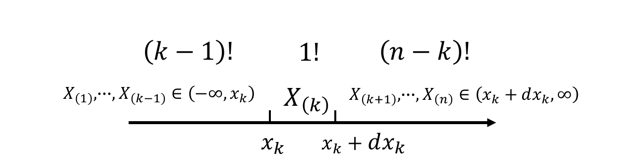
\includegraphics{2-order.png}
	\caption{次序统计量的概率微元}
	\label{Fig:order}
\end{figure}
\begin{equation}\label{Eq:ProbDiff}
	\begin{aligned}
		g({x_k}; k,n)d{x_k} = \frac{{n!}}{{(k - 1)!(n - k)!}}{[F({x_k})]^{k - 1}} f({x_k})d{x_k}{[1 - F({z_k})]^{n - k}} + o(d{x_k}) \nonumber
	\end{aligned}
\end{equation}
$g({x_k}; k,n)$即为次序统计量$X_{(k)}$的概率密度。其中,${[F({z_k})]^{k - 1}}$是前$k-1$个随机变量落入区间$(- \infty ,{x_k})$的概率;${[1 - F({x_k})]^{n - k}}$是后面$n-k$个变量落入区间$({x_k},\infty )$的概率,因为$1 - F({x_k}) = P(X > {x_k})$。 $o(d{x_k})$是$d{z_k}$的高阶无穷小量。将上式两边同时除以$d{z_k}$,则可以获得次序统计量的密度表达式
\begin{equation}
	\begin{aligned}
g({x_k};k,n) =   \frac{{n!}}{{(k - 1)!(n - k)!}} {[F({z_k})]^{k - 1}}f({x_k}){[1 - F({x_k})]^{n - k}} \nonumber
	\end{aligned}
\end{equation}
\begin{figure}[!htbp]
	\centering
	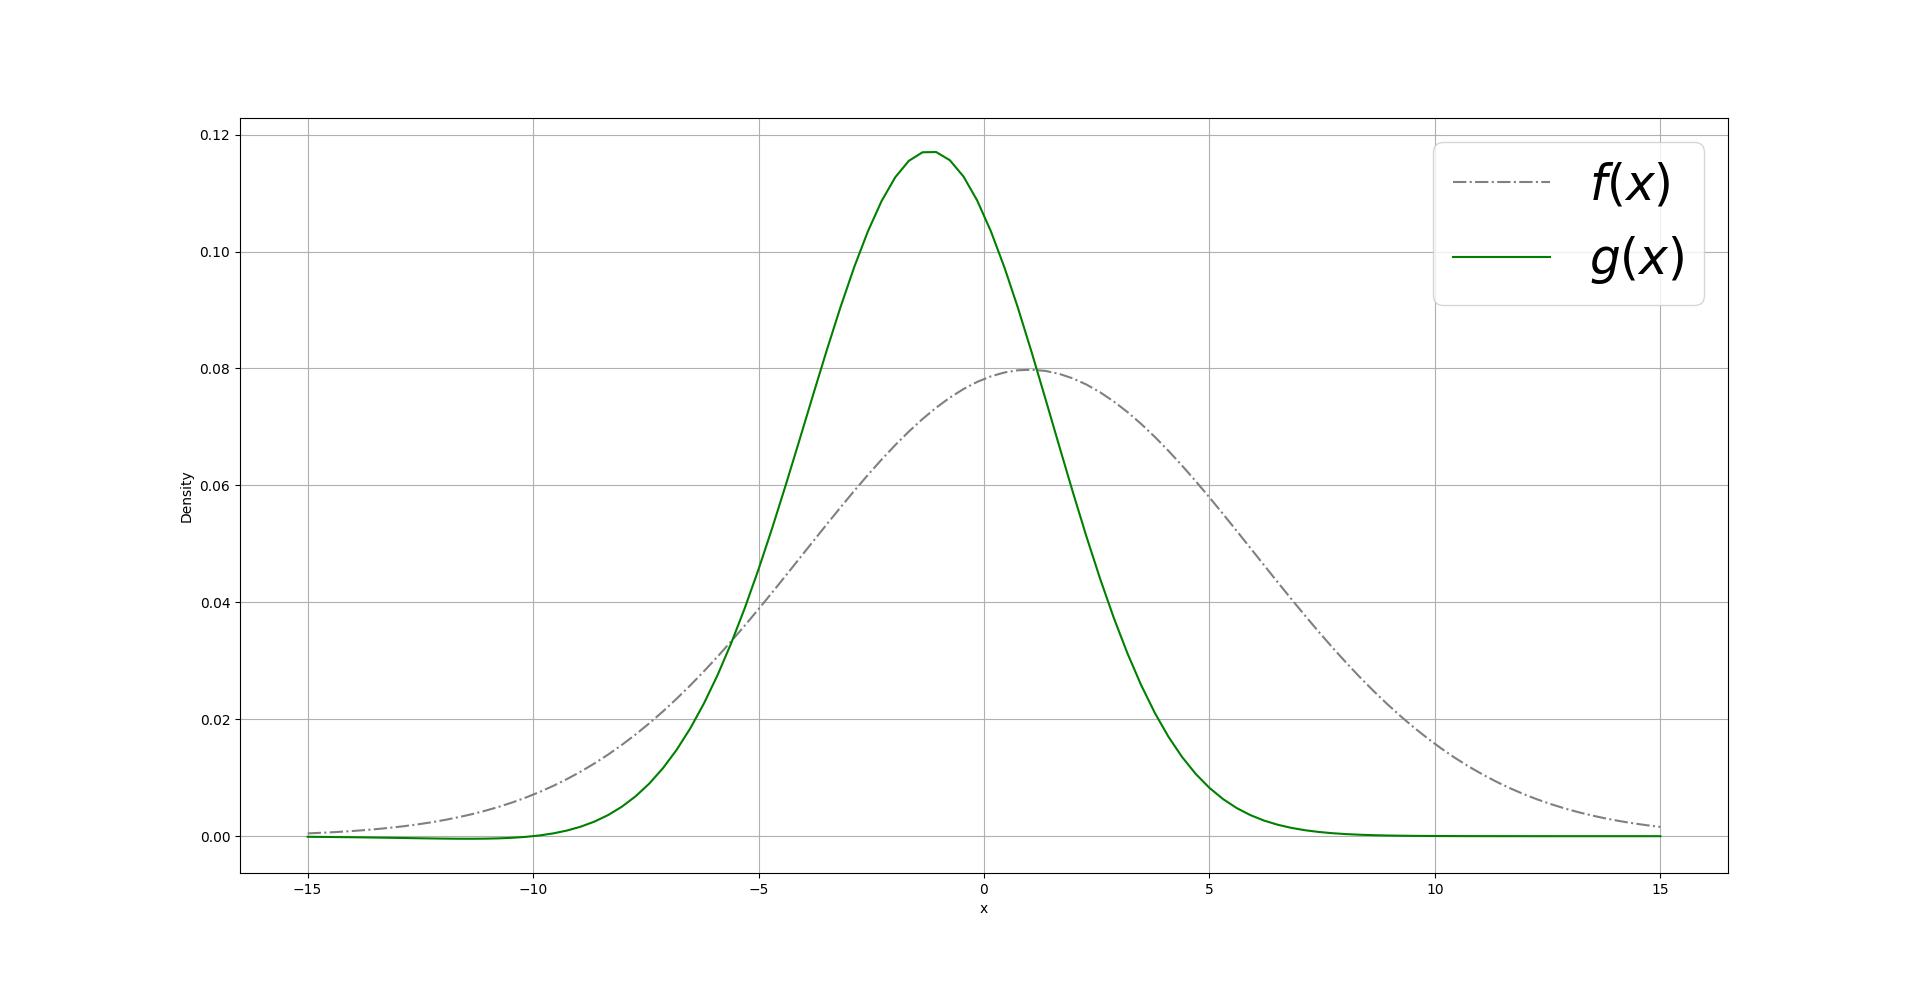
\includegraphics[width=0.6\textwidth]{order2.png}
	\caption{随机变量及其次序统计量分布示意图}
	\label{Fig:order2}
\end{figure}
上式意味着,次序统计量是随机变量分布$f(x)$的属性,只要给出随机变量的分布$f(x)$,就可以写出对应的次序统计量分布$g(x)$。图\ref{Fig:order2}给出了正态分布$\mathcal{N}(1,5)$的随机变量对应的次序统计量分布$g({x};k=2,n=5)$的示意图。可以看到,次序统计量的分布$g(x)$比$f(x)$更窄。可以使用一个例子理解这一现象:假设学生考试成绩$X$独立同分布于$f(x)$。那么在一个班级中排名最后的学生的成绩的分布可以推导为$g(x)$,其可能的成绩分数比分布$f(x)$更窄。这是因为“排名最后的学生”这个信息减少了随机变量$X$的不确定性。

如果随机变量$X$中,只包含两个总体,例如正例总体和负例总体,那么可以取$n=2$,得到次序统计量$X_{(1)}$和次序统计量$X_{(2)}$的密度为:
\begin{align}
g(x_1) &= 2 f(x) [1-F(x)] \\
g(x_2)&= 2 f(x)F(x)
\end{align}

次序统计量是非参数统计推断的最基本工具,广泛应用于诸多统计理论与实践,如分位数估计、极值分析等、排序分析等。由于个性化推荐是一个排序任务,因此次序统计量也为推荐算法提供了重要的工具。上式的两个结论,会在后面的章节多次应用。

\subsection{极大似然估计}
极大似然估计(MLE)是一种估计参数化的概率分布的方法。其基本思想是,在参数空间内,求解一个模型参数$\Theta$,使得在一次实验中观测到观测值(也称为证据)$X$的概率最大。这通过最大化似然函数来实现:
\[\arg \max p(X|\Theta)\]
其中,$p(X|\Theta)$称为似然,反映了模型参数$\Theta$对观测证据$X$的解释程度\cite{mou:2006}。以BPR为例,简单介绍极大似然估计的运作原理。给定观测到的正负样本对$X$,用户“偏好正例$i$强于负例$j$”的似然被建模为
\[p(X|\Theta) = -\log \sigma (\hat{x}_{ui} - \hat{x}_{uj})\]
其中$\hat{x}_{ui},\hat{x}_{uj}$是由用户物品特征表示$\Theta$参数化的偏好预测值。那么$p(X|\Theta)$描述了当前模型参数下,观测到用户偏好物品$i$强于$j$的概率。引入样本的独立性假设后,多个样本的似然函数是多个成对比较似然的乘积。通过对数运算将乘积运算转化为求和运算,原始的极大似然估计问题往往转化为最大化对数似然问题。

在实践中,由于要引入正则化项避免过拟合,而正则化项又等价于高斯分布先验密度的对数,因此正则化项为BPR的估计量提供了后验概率解释。
将BPR解释为极大似然估计,还是最大后验估计,主要是对正则化项的语义理解不同:若狭义地理解正则化项,那么BPR的估计量即为极大似然估计量;若把正则化项理解为高斯先验密度的对数,那么BPR为最大后验估计量。在本文成对学习的具体环境中,不区分由正则化项的语义造成的极大似然或者最大后验估计的概念差异。从贝叶斯推断的角度来看,极大似然估计通常等同于具有均匀先验分布(或标准差为无穷大的正态先验分布)的最大后验(MAP)估计\cite{beye:book}。

%极大似然通过求解参数,使得一次观测发生的概率最大化,体现的是频率学派的观点。极大似然思想也广泛体现在日常生活中,例如“要下雨(参数)了,不然不会这么闷热(观测证据)”,根据当前闷热的观测证据推断为要下雨,体现的正是极大似然原理。







%%% Local Variables:
%%% mode: latex
%%% TeX-master: t
%%% End:

\chapter{基于自适应正例去噪的推荐算法研究}
\label{cha:2}
对于个性化推荐应用而言,最广泛使用的隐式反馈是一种不完全数据(Incomplete Data),只能观察到交互的有无,而无法观察到该交互所对应偏好的大小。隐式反馈数据中通常包含一些不可信交互(误报),即伪正例,例如代购、误触等交互数据。由这些伪正例构建的成对比较,是不可信的成对比较,也称为含噪声成对比较,导致成对学习模型的不准确优化。本章提出一种自适应去噪的成对排序推荐算法(Bayesian Personalized Ranking with Autonomous Credence, BPRAC),用于从含噪成对比较的数据中学习个性化排序。由于交互对应的偏好值不可观测,本章引入一个隐变量作为衡量交互置信度的新指标,这个隐变量与用户物品表示一起作为模型参数进行端到端地学习。所提出的BPRAC算法采用期望最大化框架:在期望步骤中使用贝叶斯推断来估计交互的置信度指标;在最大化步骤中固定置信度指标,更新参数学习用户和物品的表示。在真实世界的数据集上进行的实验验证了所提出的算法的有效性。

\section{引言}
\begin{figure}[!htbp]
	\centering
	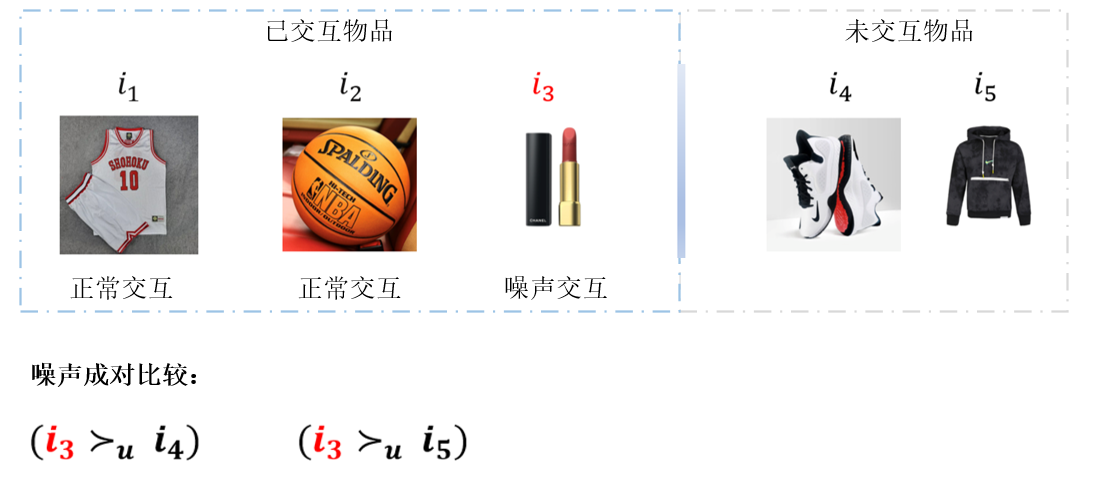
\includegraphics[width=0.6\textwidth]{2-IllustrativeExample.png}
	\caption{含噪成对比较示意图}
	\label{Fig2-1}
\end{figure}

首先用一个直观的例子阐释推荐系统中的正例噪声问题。如图~\ref{Fig2-1}所示,一个运动爱好者在节日期间购买了一个口红$i_3$作为礼物,这是一个不体现该用户偏好的偶然交互行为。但是隐式反馈数据并不包含交互所对应的偏好值,推荐模型无法识别这种不体现用户偏好的异常交互模式。成对比较是由已经交互的正例和未交互的负例构成,由于$i_3$是伪正例,任何包含$i_3$的成对比较,都是噪声成对比较。由此构成的优化目标,导致模型误认为该运动爱好者更偏好口红而非其他运动物品。协同过滤机制又会导致与口红类似的女性用品被推荐给该用户,造成过高的伪正例率。

一般而言,存在两种类型的噪声:一种是特征依赖的噪声\cite{Menon:2018:ML},例如标注者可能倾向于混淆狼和狗,但不会混淆老虎和狗,因此狼容易被错误标注而老虎不会;另外一种是独立于特征的噪声\cite{patrini:2017:CVPR},如高斯白噪声。推荐系统的误报兼具二者特征。例如误触,与物品的特征无关,每个交互的噪声率是随机分布的;而代购,则与物品的特征有关,具有礼物性质的物品更容易产生较高的噪声率。噪声来自多个方面,包括数据收集过程中的错误、不准确的标注、不完整的数据、异常值等。隐式反馈数据是典型的不完全数据,只能观测到用户的交互记录,但是无法观测到交互所对应偏好的高低。隐式反馈数据中存在一些不体现用户偏好的误触、代购等异常交互模式,和其它正常交互被无差别记录,导致了伪正例问题。噪声对机器学习模型的性能和泛化能力的负面影响体现在多个方面。首先,噪声可能导致模型对数据的过拟合。模型可能会将噪声视为真实模式,从而导致错误的学习和预测。其次,噪声可能降低模型的准确性和稳定性。如果训练数据包含大量噪声,模型可能无法准确地捕捉数据的真实分布和模式,从而导致预测结果的不可靠性。

先前的研究主要是从数据、目标函数和优化策略的角度出发解决正例噪声问题,并提出了相应的解决方法和技术。具体而言,从数据的角度,重点是通过图数据增强\cite{pmlr-v119-zheng20d,10.1145/3437963.3441734,10.1145/3437963.3441720,page1998pagerank},以获取体现原始用户物品二分图结构信息的增强图,从而有助于消除噪声正例的影响。从目标函数的角度出发,主要思路是经验风险重写(Empirical Risk Rewriting)。例如文献~\cite{liu2015classification}和文献\cite{xia:2019:NIPS}通过重加权样本,重写能够容忍噪声的损失函数,它比标准损失函数更具鲁棒性。最后,从优化策略的角度出发,重点是探索优化的动态过程,以解决标签噪声学习问题。核心在于,神经网络倾向于先拟合干净数据,然后拟合噪声数据\cite{zhang2021understanding}。基于这一发现,例如早停法~\cite{li2020gradient}作为一种简单而有效的方法,用于避免在噪声数据上过拟合;而Co-teaching方法~\cite{Han:2018:NIPS}通过小损失技巧相互筛选干净样本,鲁棒地同时训练两个网络。

在成对学习的问题设置下,正例噪声问题更具挑战性。从优化策略出发的“神经网络倾向于先拟合干净数据,然后拟合噪声数据”的经验性观察主要是基于单个样本构建的损失,是否在成对样本构建的损失上依旧起作用是存疑的,因为在推荐中往往是难以拟合的困难样本对性能的提升贡献越大\cite{Steffen:2014:WSDM}。从数据角度出发的图数据增强可能会损失图中重要的结构信息,因为随机丢弃的点或者边可能会体现图的重要结构信息,从而引入新的噪声。从目标函数角度出发的经验函数重写,主要是基于以均方误差等为代表点式损失(pointwise)损失,这类损失在单个样本和标签上构建,难以向对比损失推广。

回溯伪正例的本质,是隐式反馈数据的特性造成的
:它是一种不完全数据,无法观测到交互所对应的偏好值,才产生了噪声成对比较。如果能观测到每个交互偏好强度的高低,那么根据偏好值大小值构造的成对比较就是可靠的。从统计视角,期望-最大化(Expectation-Maximazation)最大化框架是一个从不完全数据中进行极大似然或者最大后验估计非常有效的方法,可以估计无法观测到的隐变量和模型参数。因此,本章引入一个隐变量,含义为每个交互的偏好值,同时也对应了每个成对比较置信度的高低,交互的偏好值越大则成对比较的置信度越高,并端到端地学习模型参数和置信度指标:在期望步骤中使用贝叶斯推断来估计置信度指标;在最大化步骤中固定置信度指标,更新模型参数学习用户和物品的表示,以减少噪声成对比较对学习算法的影响,学习更加准确的用户和物品表示。

本章对推荐系统的正例去噪研究做出了如下贡献:(1)将从噪声成对比较中学习排序形式化为一个含有隐变量的最大后验估计问题;(2)贡献了基于次序统计量的排序分析的隐变量估计方法。

\section{自适应正例去噪算法设计}
\subsection{问题设置}
设$\mathbf{X}=[x_{ui}] \in \mathbb{R}^{M\times N}$表示包含$M$个用户和$N$个物品的交互矩阵,其中$x_{ui}\in \{1,0\}$。令$\mathcal{U}$和$\mathcal{I}$分别表示用户集合和物品集合。对于用户$u \in \mathcal{U}$,令$\mathcal{I}_u^+ \subseteq \mathcal{I}$表示他交互过的物品集合,$\mathcal{I}_u^- = \mathcal{I}\backslash \mathcal{I}_u^+$表示他未交互过的物品集合。通过选择一个属于$\mathcal{I}_u^+$的物品$i$和一个属于$\mathcal{I}_u^-$的物品$j$,可以构建成对比较的实例。训练数据集可以通过以下方式构建:
\begin{equation}\label{Eq2:obj}
	\mathcal{D} =  \left\{ {(u,i,j)|i \in \mathcal{I}_u^ +  \wedge j \in \mathcal{I}_u^ - } \right\}.
\end{equation}

BPR的目标是从训练数据集中学习用户和物品表示$\Theta$,使得观测到$\mathcal{D}$的后验概率最大化,即:
\begin{equation}\label{Eq:BPRObjective}
\mathcal{L}_\textsc{BPR} = \prod_{(u,i,j) \in \mathcal{D}} P(i \succ_u j|\Theta)P(\Theta).
\end{equation}
如果一个交互$x_{ui}=1$是噪声(伪正例),则所有包含$i$的成对比较$i \succ_u j$即为噪声比较,它们描述了不准确的用户偏好结构。这些噪声成对比较不应该包含在最大后验目标之内,否则会学到不准确的用户物品表示。然而,由于无法观测哪些交互是可信的,因此引入新的参数$c_{ui}$作为隐变量来衡量成对比较$i \succ_u j$的置信度。具体而言,对于一个可信的交互,$c_{ui}=1$;否则,$c_{ui}=0$。那么可以修正BPR的优化目标为:
\begin{equation}\label{Eq:Objective}
\mathcal{L}\prime = \prod_{(u,i,j) \in \mathcal{D}} [P(i \succ_u j|\Theta)P(\Theta)]^{c_{ui}}.
\end{equation}
其中,$c_{ui}$是隐藏变量,对交互项$(u,i)$进行加权。当$c_{ui} \rightarrow 0$(即不可信的交互)时,噪声比较$i \succ_u j$的后验概率被固定为1,用户和物品表示$\Theta$的更新不受该噪声成对比较的影响。作为一个可学习的变量,隐变量$c_{ui}$提供了从噪声数据中进行表示学习的解决方案。从含噪成对比较中学习排序的问题,可以形式化为一个含有隐变量的最大后验估计问题。

跟随BPR论文的符号规则,使用$\hat{x}_{ui}$来表示用户$u$对物品$i$的偏好预测值。用户偏好物品$i$超过物品$j$的似然为:
\begin{equation}\label{Eq2:Sigma}
	P(i \succ_u j | \Theta) = \sigma(\hat{x}_{ui} - \hat{x}_{uj}),
\end{equation}
其中,$\sigma(\cdot)$是sigmoid函数:$\sigma(z) = \frac{1}{1+e^{-z}}$。将公式\eqref{Eq2:Sigma}带入公式\eqref{Eq:Objective}中,并两边取对数,得到了如下最终的优化目标:
\begin{equation}\label{Eq:LogObjective}
\ln	\mathcal{L}\prime = \sum_{(u,i,j) \in \mathcal{D}} c_{ui}\left[\ln \sigma(\hat{x}_{ui} - \hat{x}_{uj}) - \lambda \|\Theta\|^2 \right],
\end{equation}
其中,$\lambda \|\Theta\|^2$是模型训练中的正则化项。下面介绍在矩阵分解模型下,如何求解这个含有隐变量的最大后验估计问题。
\subsection{先验分布}
本节的目标是获取BPR设定下的相似度分数的概率分布。BPR论文设定了用户物品表示为两个$d$维高斯随机向量的内积,基于矩阵分解得到的相似度分数先验分布由如下引理给出。
\begin{lemma}\label{Lemma2:AprioriDistribution}
设$x=\langle \mathbf{w}, \mathbf{h} \rangle$表示两个$d$维随机向量的内积,其中$\mathbf{w}$和$\mathbf{h}$的元素是独立同分布的随机变量,每个随机变量都服从$\mathcal{N}(0, \lambda)$的高斯分布。那么$x$的概率密度函数(PDF)为:
	\begin{equation}
		f_{X}(x; d, \lambda) = \frac{1}{\lambda \sqrt{\pi} \Gamma(\frac{d}{2})}\left(\frac{|x|}{2\lambda} \right)^{\frac{d-1}{2}}K_{\frac{d-1}{2}}\left(\frac{|x|}{\lambda}\right),
	\end{equation}
	其中,$K_{\eta}(\cdot)$是第三类修正的贝塞尔函数,$\Gamma(\cdot)$是伽玛函数。
\end{lemma}
\begin{proof}
随机变量$x=\langle \mathbf{w}, \mathbf{h} \rangle$可以通过以下代数运算转化为两个伽玛分布的随机变量的差:
\begin{eqnarray}
	x &=& \langle {\mathbf{w}},{\mathbf{h}} \rangle = \sum\nolimits_{k = 1}^d {w_k} \cdot {h_{k}} \nonumber\\
	&=& \frac{{{\lambda }}}{2}\sum\nolimits_{k = 1}^d {[\frac{{{{({w_{k}} + {h_{k}})}^2}}}{{2{\lambda  }}} - } \frac{{{{({w_{k}} - {h_{k}})}^2}}}{{2{\lambda  }}}]
\end{eqnarray}
那么
\begin{equation}
	\frac{2}{{{\lambda  }}}x = \sum_{k = 1}^{d} \frac{{{{({w_{k}} + {h_{k}})}^2}}}{{2{\lambda }}} - \sum_{k = 1}^{d} \frac{{{{({w_{k}} - {h_{k}})}^2}}}{{2{\lambda  }}},
\end{equation}
其中 $\frac{(w_k + h_k)}{\sqrt {2{\lambda}}} \sim \mathcal{N}(0,1)$, $\frac{(w_k - h_k)}{\sqrt {2{\lambda}}} \sim \mathcal{N}(0,1)$. 于是第一项${z_1} = \sum\nolimits_{k = 1}^d {\frac{{{{({w_{k}} + {h_{k}})}^2}}}{{2{\lambda }}}} $ 和第二项 ${z_2} = \sum\nolimits_{k = 1}^d {\frac{{{{({w_{k}} - {h_{k}})}^2}}}{{2{\lambda }}}} $ 服从自由度为$d$的卡方分布。 注意到卡方分布${\chi ^2}(d)$ 是参数为$Ga(z;\frac{d}{2},\frac{1}{2})$的伽玛分布族的特例, 因此变量${Z_1}$ and $ - {Z_2}$ 的特征函数为:
%a3
\begin{align}
	{\phi _{{Z_1}}}(t) &= {(1 - 2it)^{ - \frac{d}{2}}}, \\
	{\phi _{ - {Z_2}}}(t) &= {(1 + 2it)^{ - \frac{d}{2}}},
\end{align}
其中 $i$ 为虚数单位。 进一步地,记随机变量 $Y = \frac{2}{{{\lambda }}}X  = {Z_1} + ( - {Z_2})$, 则随机变量Y的特征函数 ${\phi _Y}(t)$是${\phi _{{Z_1}}}(t)$ 和 ${\phi _{ - {Z_2}}}(t)$的乘积:
\begin{equation}
	{\phi _Y}(t) = {\phi _{{Z_1}}}(t) \cdot {\phi _{ - {Z_2}}}(t) = {(1 + 4{t^2})^{ - \frac{d}{2}}}.
\end{equation}
那么随机变量Y的概率密度函数${f_Y}(y)$可以通过如下傅里叶逆变换计算得到:
\begin{eqnarray}
		{f_Y}(y) &=& \frac{1}{{2\pi }}\int_{ - \infty }^\infty  {{\phi _Y}(t){e^{ity}}dt} \nonumber\\
		& =& \frac{1}{{2\pi }}\int_{ - \infty }^\infty  {{{(1 + 4{t^2})}^{ - \frac{d}{2}}}{e^{ity}}dt}.
\end{eqnarray}

\par
直接计算上式${f_Y}(y)$是复杂的。观察到特征函数${\phi_Y}(t)$与方差伽玛(VG)分布~\cite{Madan:1990:Business,Senata:2004:ApplyPro}的特征函数具有相同的函数形式。VG分布的特征函数为
\begin{equation}
	{\phi _{VG}}(t) = E({e^{itX}}) = {e^{i\delta t}}{(1 - i\theta vt + \frac{{{\sigma ^2}v}}{2}{t^2})^{ - {1 \mathord{\left/
					{\vphantom {1 v}} \right.
					\kern-\nulldelimiterspace} v}}}.
\end{equation}
VG分布的概率密度函数${f_{VG}}(y)$为:
\begin{equation}
	\begin{aligned}
		{f_{VG}}(y;\theta ,\delta ,\sigma ,v) = \frac{{2e\frac{{\theta (y - \delta )}}{{{\sigma ^2}}}}}{{\sigma \sqrt {2\pi } {v^{\frac{1}{v}}}\Gamma (\frac{1}{v})}}{(\frac{{|y - \delta |}}{{\sqrt {\frac{{2{\sigma ^2}}}{v} + {\theta ^2}} }})^{\frac{1}{v} - \frac{1}{2}}}
		\cdot {{\rm K}_{\frac{1}{v} - \frac{1}{2}}}(\frac{{|y - \delta |\sqrt {\frac{{2{\sigma ^2}}}{v} + \theta } }}{{{\sigma ^2}}}).
	\end{aligned}
\end{equation}
取$\delta$=0, $\theta $=0, $v$=2/d, $\sigma$=$2\sqrt d$,那么
\begin{equation}
	{\phi _{VG}}(t) = {(1 + \frac{1}{4}{t^2})^{ - \frac{d}{2}}} = {\phi _Y}(t),
\end{equation}
由于特征函数与概率密度函数是一一对应的关系,因此Y的概率密度函数为
\begin{eqnarray}
		{f_Y}(y) &=& {f_{VG}}(y;\theta  = 0,\delta  = 0,\sigma  = 2\sqrt d ,v = \frac{2}{d})\nonumber\\
		& =& \frac{1}{{\sqrt {2\pi d} {{\left( {\frac{2}{d}} \right)}^{\frac{d}{2}}}\Gamma (\frac{d}{2})}}{(\frac{{|y|}}{{2d}})^{\frac{{d - 1}}{2}}}{{\rm K}_{\frac{{d - 1}}{2}}}(\frac{{|y|}}{2})\nonumber\\
		& =& \frac{1}{{\sqrt {2\pi } {2^{\frac{d}{2}}}\Gamma (\frac{d}{2})}}{(\frac{{|y|}}{2})^{\frac{{d - 1}}{2}}}{{\rm K}_{\frac{{d - 1}}{2}}}(\frac{{|y|}}{2}).
\end{eqnarray}

\par
需要注意的是,$\frac{{{\lambda }}}{2}Y = X$。通过将$Y$按照常数$\rho$进行缩放,可以生成一个经过缩放的随机变量分布
\begin{equation}
	\rho Y \sim \frac{1}{\rho }{f_Y}(\frac{y}{\rho }).
\end{equation}
取 $\rho  = \frac{{{\lambda  }}}{2}$,则$X = \frac{{{\lambda }}}{2}Y \sim \frac{2}{{{\lambda }}}{f_Y}(\frac{2}{{{\lambda }}}y)$,进而可以得到随机变量$X$的概率密度函数为:
\begin{equation}
	f_{X}(x; d, \lambda) = \frac{1}{\lambda \sqrt{\pi} \Gamma(\frac{d}{2})}\left(\frac{|x|}{2\lambda} \right)^{\frac{d-1}{2}}K_{\frac{d-1}{2}}\left(\frac{|x|}{\lambda}\right),
\end{equation}
\end{proof}
在BPR中,论文假设参数用户和物品的表示$\Theta$服从零均值和对角协方差矩阵的多元高斯分布,那么参数矩阵$\Theta$的所有元素都是独立且同分布(i.i.d)的随机变量,每个随机变量都服从$\mathcal{N}(0, \lambda)$的高斯分布。按照如上的多元高斯分布初始化后,使用引理\ref{Lemma2:AprioriDistribution}的结果,可以得到基于矩阵分解的偏好预测值的分布为:
\begin{equation}\label{Eq:PDFInnerProduct}
	f(\hat{x}_{ui}) = \frac{1}{\lambda \sqrt{\pi} \Gamma(\frac{d}{2})}\left(\frac{|\hat{x}_{ui}|}{2\lambda} \right)^{\frac{d-1}{2}}K_{\frac{d-1}{2}}\left(\frac{|\hat{x}_{ui}|}{\lambda}\right),
\end{equation}
相应的累积分布函数(CDF)为:
\begin{equation}\label{Eq:CDFInnerProduct}
	F(\hat{x}_{ui}) = \int_{-\infty}^{\hat{x}_{ui}} f(t)d(t).
\end{equation}

图\ref{Fig:Prior}描绘了公式~\eqref{Eq:PDFInnerProduct}和公式~\eqref{Eq:CDFInnerProduct}给出了不同参数下,高斯随机向量内积相似度的概率密度函数及相应的累计分布函数,满足概率分布的正定性和归一性条件。
\begin{figure*}[h!]
	\centering
	\subfloat{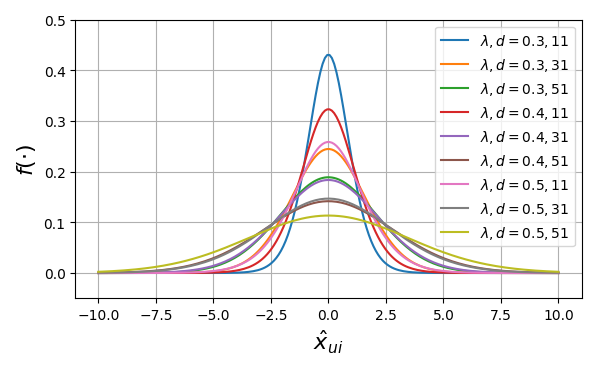
\includegraphics[width=.6\textwidth]{2-PriorPDF.png}}\\
	\subfloat{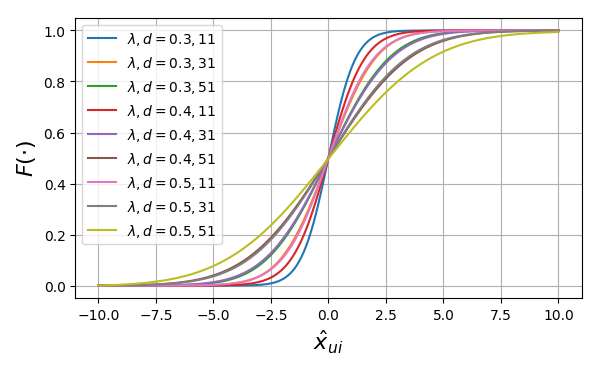
\includegraphics[width=.6\textwidth]{2-PriorCDF.png}}
	\caption{不同参数下先验分布的概率密度及累积分布函数示意图}
	\label{Fig:Prior}
\end{figure*}

\subsection{真正例相似度分数的分布}\label{Sec:Posterior}
本节的目标是获取真正例相似度观测值的分布。
%考虑$n$个独立同分布的随机变量$\{Z_i\}_{i=1}^n$,其对应的取值$\{z_i\}_{i=1}^n$按升序排列:$X_1 \le X_2 \le \cdots X_n$,其中$X_k$是取值$x_k$在第$k$个位置的随机变量,那么$x_k$的概率密度为
%\begin{equation}\label{Eq:PosteriorPDF}
%	\begin{aligned}
%		g({x_k};k,n)
%		=   \frac{{n!}}{{(k - 1)!(n - k)!}} {[\Phi({x_k})]^{k - 1}}\phi({x_k}){[1 - \Phi({x_k})]^{n - k}}.
%	\end{aligned}
%\end{equation}
对于一个交互,只存在两种可能:(1)它是真正例,即用户真的喜欢;(2)它是伪正例,即用户不喜欢。预测评分只存在两个总体,于是取$n=2$。此外,模型是针对负例评分小于正例评分优化,对于真正例的预测评分$\hat{x}_{ui}$,如果它是用户喜欢的正例,应该满足$\hat{x}_{uj}\leq \hat{x}_{ui}$。把这两个随机变量按升序排列,真正例的预测评分$\hat{x}_{ui}$在两个随机变量中排序第二,这正是次序统计量$X_{(2)}$的取值。根据第\ref{cha:intro1}章第\ref{order}部分关于次序统计量的预备知识,可以写出真正例的预测评分$\hat{x}_{ui}$的分布
\begin{eqnarray}\label{Eq:ConditionalDistribution}
	g(\hat{x}_{ui};k=2,n=2)
	& = & 2 F(\hat{x}_{ui})f(\hat{x}_{ui}),
\end{eqnarray}
其中 $f(\cdot)$由公式\ref{Eq:PDFInnerProduct}给出,$F(\cdot)$由公式\ref{Eq:CDFInnerProduct}给出。

图\ref{Fig:Posterior}绘制了不同参数下,可信交互(真正例)预测偏好值的分布示意图,可以看到它也满足概率分布的非负性和归一性条件。

\begin{figure*}[t]
	\centering
	\subfloat{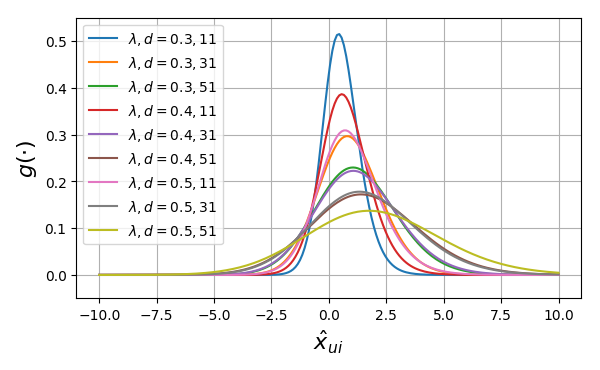
\includegraphics[width=.6\textwidth]{2-PosteriorPDF.png}}\\
	\subfloat{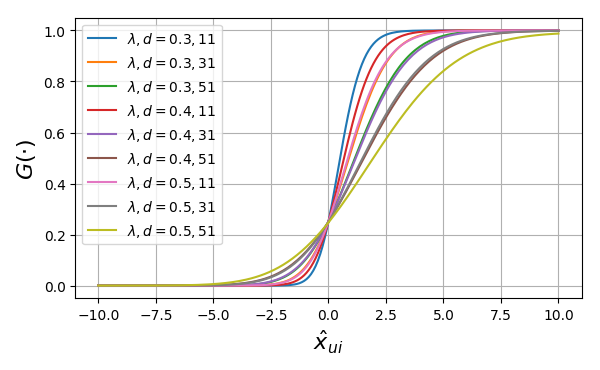
\includegraphics[width=.6\textwidth]{2-PosteriorCDF.png}}
	\caption{不同参数下后验分布的概率密度及累积分布函数示意图}
	\label{Fig:Posterior}
\end{figure*}

\subsection{学习算法}
在本节中,介绍自适应去噪的成对排序学习算法,并分析了其收敛性。由于这是一个含有隐变量的最大后验估计问题,因此使用EM算法\cite{Dempster:1977:RSS}进行端到端地估计隐变量并学习模型参数。具体而言,包括两个步骤:(i) 在期望步骤中估计$c_{ui}$,以及(ii) 在最大化步骤中学习用户和物品表示$\Theta$。

\subsubsection{期望步骤}
\newpage
在期望步骤中,固定的模型参数$\Theta$,即给定预测评分,目标是估计$c_{ui}$。首先写出$Q(\cdot)$函数\cite{Dempster:1977:RSS}为 
\begin{eqnarray}\label{Eq:QDef}
 Q(\Theta, \Theta^{(t)}) 
	& = & \mathbb{E}_{c_{ui} } \left[ \ln P(\Theta|\succ_u, c_{ui}) | \succ_u, \Theta^{(t)} \right] \nonumber \\
	& = & \mathbb{E}_{c_{ui}} \left[ \Sigma_{(u,i,j)\in \mathcal{D}} c_{ui} \left( \ln \sigma(\hat{x}_{ui} - \hat{x}_{uj}) - \lambda \| \Theta \|^2 \right) \right] \nonumber \\
	& = & \Sigma_{(u,i,j) \in \mathcal{D}} \mathbb{E}[c_{ui}] \left[ \ln \sigma(\hat{x}_{ui} - \hat{x}_{uj}) - \lambda \| \Theta \|^2 \right],
\end{eqnarray}
其中,$\mathbb{E}[c_{ui}]$是给定在第$t$次学习迭代中模型参数$\Theta^{(t)}$的条件下,$c_{ui}$的期望值。使用$\mathbb{E}[c_{ui}]$作为$c_{ui}$的估计。由于$c_{ui}$是一个二值伯努利变量,有以下关系式:

\begin{align}
 \hat{c}_{ui}=	\mathbb{E}[c_{ui}] &= P({c_{ui}} = 1|\Theta,{ \succ _u}) \nonumber \\
	&= P({c_{ui}} = 1|{\hat{x}_{ui}} ,\succ_u)  \label{Eq:EStimationCui} \\
	&= \frac{ P( {\hat{x}_{ui}},{ \succ_u}|{c_{ui}} = 1)}{ P({\hat{x}_{ui}} ,\succ_u)}{P({c_{ui}} = 1)} \label{Eq:Bayes}\\
	&\propto P( {\hat{x}_{ui}},{ \succ_u}|{c_{ui}} = 1)P({c_{ui}} = 1) \label{Eq:Bayesian} \\
	&= g({{\hat x}_{ui};n=2,k=2})P({c_{ui}} = 1) \label{Eq:ClassDensity}
\end{align}
$\succ_u$是BPR\cite{Steffen:2009:UAI}所定义的偏好结构,意为$\hat{x}_{uj}\leq \hat{x}_{ui}$。当固定模型参数$\Theta$时,预测评分$\hat{x}_{ui}$也被固定,于是有公式\eqref{Eq:EStimationCui}。式\eqref{Eq:Bayes}是基于贝叶斯公式得到,其中$P(c_{ui}=1)$是交互为可信的先验概率,分母$P(\hat{x}_{ui},\succ_u)$在贝叶斯分析中被省略为归一化常数。$P(\hat{x}_{ui},\succ_u|c_{ui}=1)$是可信交互的概率密度。给定所有的预测评分,对于一个可信的交互$(u,i)$,其预测评分$\hat{x}_{ui}$应该满足$\hat{x}_{uj} \leq \hat{x}_{ui}$,此时概率密度由公式\eqref{Eq:ConditionalDistribution}给出。在给定$P(c_{ui}=1)$的情况下,观测值$\hat{x}_{ui}$在分布$g({{\hat x}_{ui};n=2,k=2})$中对应的概率密度越高,它是可信交互的可能性越大。

设$n_i$表示物品$i$的选择比例,即与该物品进行交互的用户的百分比。令$\bar{n}$和$\sigma_n$分别表示交互比例的平均值和标准差。通过以下方式计算$P(c_{ui} =1)$:
\begin{eqnarray}
	P(c_{ui} =1) = \mathsf{sigmoid}(\frac{n_i - \bar{n} }{\sigma_n}).
\end{eqnarray}
其中$\mathsf{sigmoid}$函数的作用是将输入转换为$(0,1)$范围内的概率。该公式的直观解释是,一个物品的交互比例越高,越多用户交互,那么它是可信交互的先验概率越大。

\subsection{最大化步骤}
在最大化步骤中,固定隐变量$\hat{c}_{ui}$, 然后学习模型参数$\Theta$以最大化$Q(\cdot)$函数,即
\begin{equation}\label{Eq:MaxQFunction}
	\arg \mathop {\max }\limits_\Theta  \sum\nolimits_{(u,i,j) \in \mathcal{D}} {{{\hat c}_{ui}}[\ln \sigma ({{\hat x}_{ui}} - {{\hat x}_{uj}}) - {\lambda  }\|\Theta\|^2]}.
\end{equation}

\par
采用广泛使用的随机梯度下降(SGD)技术来学习模型参数。对于每个训练三元组$(u,i,j)$,其梯度为:
\begin{equation}\label{Eq:Gradient1}
	\frac{{\partial Q(\Theta, \Theta^{(t)} )}}{{\partial \Theta }} = \sum\nolimits_{(u,i,j) \in \mathcal{D}} \hat{c}_{ui} [ (1 - \sigma(\hat{x}_{ui}-\hat{x}_{uj}))\frac{\partial\hat{x}_{uij}}{\partial\Theta} - \lambda\Theta ],
\end{equation}
其中
\begin{equation}\label{Eq:Gradient2}
	\frac{{\partial {{\hat x}_{uij}}}}{{\partial \Theta }} = \frac{{\partial ({{\hat x}_{ui}} - {{\hat x}_{uj}})}}{{\partial \Theta }} = \left\{ {\begin{array}{*{20}{l}}
			{\mathbf{h}}_i - \mathbf{h}_j,\\
			{\mathbf{w}}_{u},\\
			{ - \mathbf{w}}_{u},
		\end{array}\begin{array}{*{20}{l}}
			{\mathrm{if} \;\; \theta  = {\mathbf{w}}_u}\\
			{\mathrm{if} \;\; \theta  = {\mathbf{h}}_i}\\
			{\mathrm{if} \;\; \theta  = {\mathbf{h}}_j}.
	\end{array}} \right.
\end{equation}
$\theta$表示$\mathbf{W}$或$\mathbf{H}$的特定行或者列。给定正则化参数$\alpha$,以及正则化常数$\lambda$,模型参数的更新规则为
\begin{equation}\label{Eq:Updating}
	\Theta  \leftarrow \Theta  + \alpha \hat{c}_{ui} [ (1 - \sigma(\hat{x}_{ui}-\hat{x}_{uj}))\frac{\partial\hat{x}_{uij}}{\partial\Theta} - \lambda\Theta ].
\end{equation}
\section{算法实现与时间复杂度分析}
\subsection{伪代码}
从公式\eqref{Eq:Updating}可以看出,新的参数$c_{ui}$充当了动态学习率的角色,实质上重新加权了具有较高偏好水平的交互,并为学习算法过滤了具有较低偏好水平的噪声交互。算法的实现使用了EM框架,在E步固定模型参数求解隐变量,在M步固定隐变量学习模型参数。算法~\ref{Alg2:1}给出了BPRAC学习算法的伪代码。
\begin{algorithm}[t]
	\counterwithin{algorithm}{chapter}
	\SetKwInput{KwIn}{输入}  %<---细节与重点
	\SetKwInput{KwOut}{输出}  %<---细节与重点
	\SetAlgoLined
	\small
	\caption{自适应去噪的成对学习排序算法伪码}\label{Alg2:1}
	\KwIn{交互集合$\mathcal{S}$, 训练三元组集合$\mathcal{D}$, 最大迭代轮数$T$, 抽样的训练三元组数量$K$。}
	\KwOut{预测的评分矩阵$\mathbf{X} \in \mathbb{R}^{M \times N}$。}
	初始化特征表示$\Theta =(\mathbf{W}, \mathbf{H})$,其中$\mathbf{w}_u \sim \mathcal{N}(0, \lambda \mathbf{I})$,$\mathbf{h}_i \sim \mathcal{N}(0, \lambda \mathbf{I})$ ;
	
	\For{$t = 1; t \le T; t$++}
	{
		\textit{\# Expectation步: 固定$\Theta$, 计算隐变量${{\hat c}_{ui}}$};
		
		\For{每一个交互$(u,i) \in \mathcal{S}$}
		{
			~~计算预测评分${{\hat x}_{ui}} = \left\langle   {{\mathbf{w}_u},{\mathbf{h}_i}} \right\rangle  $;\\
			通过公式~\eqref{Eq:PDFInnerProduct}计算先验分布$f({{\hat x}_{ui}})$;\\
			通过公式~\eqref{Eq:CDFInnerProduct}计算$F({{\hat x}_{ui}})$ ;\\
			通过公式~\eqref{Eq:ConditionalDistribution}计算后验分布$g({{\hat x}_{ui}};k=2,n=2)$;\\
			通过公式~\eqref{Eq:ClassDensity}计算${{\hat c}_{ui}}$;
		}
		\textit{\# Maximization步: 固定${{\hat c}_{ui}}$, 更新参数$\Theta$};
		
		\For{$k=1; k\le K; k$++}
		{
			~~抽样一个三元组$(u,i,j) \in \mathcal{D}$;\\
			计算预测评分${{\hat x}_{ui}}$,${{\hat x}_{uj}}$ ;\\
			通过公式~\eqref{Eq:Updating}执行梯度下降更新参数$\Theta$;
		}
	}
	\KwResult{$\mathbf{X}=\mathbf{W}\times {\mathbf{H}^\mathsf{T}} $。}
\end{algorithm}

\subsection{时间复杂度分析}
由于E步对隐变量的估计是标量计算,因此时间复杂度是$\mathcal{O}(|\mathcal{S}|)$,其中$|\mathcal{S}|$是训练集中交互总数。而M步主要是向量的梯度下降,因此M步的时间复杂度是$\mathcal{O}(|\mathcal{D}|d)$,其中,$|\mathcal{D}|$是三元组的数量,$d$是嵌入的维度。由于$|\mathcal{S}| \le\le (|\mathcal{D}|)$,即交互数远小于训练三元组的数量,因此自适应去噪的成对排序算法的时间复杂度主要源自于M步:固定隐变量,学习用户和物品的特征表示,即执行一次最外层循环的时间复杂度为$\mathcal{O}(|\mathcal{D}|d)$,这也是标准的BPR的时间复杂度。由于最外层要执行T次循环,总体的计算复杂度为$\mathcal{O}(T|\mathcal{D}|d)$,其中$T$是学习迭代的次数。

\section{收敛性分析}\label{Sec:Convergence}
在期望步骤中,使用$\mathbb{E}[c_{ui}] \propto \hat{c}_{ui}$的近似来计算$c_{ui}$的估计值。从公式\eqref{Eq:Updating}中可以直观地观察到,由于$\hat{c}_{ui} \ge 0$,$\hat{c}_{ui}$的近似仅改变参数更新过程中的步长,而不改变参数更新的方向,也就是说这个近似只改变了梯度下降过程中通往(局部)最小值的步长,但并不会改变梯度更新的方向,因此并不会改变算法的收敛性。BPRAC算法的收敛性的严格证明由如下引理给出。
\begin{lemma}\label{Lemma:ConvergenceAnalysis}
给定所有的成对比较 ${\succ _u}$,记后验概率序列为$P(\Theta^{(t)} |\succ_u)$,其中${\Theta ^{(t)}}(t=1,2,...)$为第$t$训练轮次学到的用户物品表示。那么,后验概率${P(\Theta ^{(t)}|\succ_u)}$收敛,且
	\begin{equation}\label{Eq:PosteriorSupremum}
		\mathop {\lim }\limits_{t \to \infty } P({\Theta ^{(t)}}|{ \succ _u}) = \sup \{ P({\Theta ^{(t)}}|{ \succ _u}) | t \in \mathbb{N}\}.
	\end{equation}
\end{lemma}

\begin{proof}
首先证明$\mathbb{E}[c_{ui}] \propto {{\hat c}_{ui}} $的这个近似不改变后验概率序列的非递减性质,也就是说要证明
\begin{equation}\label{eq20}
	P({\Theta ^{(t + 1)}}|{ \succ _u}) \ge P({\Theta ^{(t)}}|{ \succ _u}).
\end{equation}

\par
根据全概率公式,有
\begin{equation}\label{eq21}
	\begin{split}
		P(\Theta |{ \succ _u}) &= \frac{{P(\Theta ,c|{ \succ _u})}}{{P(c|\Theta ,{ \succ _u})}}\\
		& = \frac{{P(\Theta |c,{ \succ _u})P(c|{ \succ _u})}}{{P(c|\Theta ,{ \succ _u})}}.
	\end{split}
\end{equation}
因此
\begin{equation}\label{eq22}
	\begin{aligned}
		\log P(\Theta |{ \succ _u}) = \log P(\Theta |c,{ \succ _u}) - \log P(c|\Theta ,{ \succ _u})
		+ \log P(c|{ \succ _u}).
	\end{aligned}
\end{equation}
定义:
\begin{equation}\label{eq23}
	\begin{split}
		Q(\Theta ,{\Theta ^{(t)}}) &= {\mathbb{E}_{{c_{ui}}}}[\log P(\Theta |c,{ \succ _u})|{ \succ _u},{\Theta ^{(t)}}],\\
		H(\Theta ,{\Theta ^{(t)}}) &= {\mathbb{E}_{{c_{ui}}}}[\log P(c|\Theta ,{ \succ _u})|{ \succ _u},{\Theta ^{(t)}}],\\
		K(\Theta ,{\Theta ^{(t)}}) &= {\mathbb{E}_{{c_{ui}}}}[\log P(c|{ \succ _u})|{ \succ _u},{\Theta ^{(t)}}].
	\end{split}
\end{equation}
于是
\begin{equation}\label{eq24}
	\log P(\Theta |{ \succ _u}) \buildrel \Delta \over = Q(\Theta ,{\Theta ^{(t)}}) - H(\Theta ,{\Theta ^{(t)}}) + K(\Theta ,{\Theta ^{(t)}}).
\end{equation}
那么后验概率序列的差值为:
\begin{equation}\label{eq25}
	\begin{aligned}
		\log P({\Theta ^{(t + 1)}}|{ \succ _u}) - \log P({\Theta ^{(t)}}|{ \succ _u})
		= [Q({\Theta ^{(t + 1)}},{\Theta ^{(t)}}) - Q({\Theta ^{(t)}},{\Theta ^{(t)}})] \\
		- [H({\Theta ^{(t + 1)}},{\Theta ^{(t)}}) - H({\Theta ^{(t)}},{\Theta ^{(t)}})].
	\end{aligned}
\end{equation}

\par
在期望步骤中,采用了$\mathbb{E}[c_{ui}] \propto \hat{c}_{ui}$的近似方法。假设$\hat{c}_{ui} = \text{const} \cdot \mathbb{E}[c_{ui}]$,其中$\text{const} > 0$。根据最大化步骤,
\begin{equation}\label{eq26}
	\begin{split}
		{\Theta ^{(t+1)}} =& \arg \mathop {\max }\limits_\Theta  \sum\nolimits_{(u,i,j) \in {D_S}} {{{\hat c}_{ui}}[\ln \sigma ({{\hat x}_{ui}} - {{\hat x}_{uj}})}
		{- {\lambda _\Theta }||\Theta |{|^2}]}
		\\=& \arg \mathop {\max }\limits_\Theta  \sum\nolimits_{(u,i,j) \in {D_S}} {const \cdot E({c_{ui}})[\ln \sigma ({{\hat x}_{ui}} }
		{- {{\hat x}_{uj} )}- {\lambda _\Theta }||\Theta |{|^2}]}
		\\=& \arg \mathop {\max }\limits_\Theta  const \cdot Q(\Theta ,{\Theta ^{(t)}}).
	\end{split}
\end{equation}
\par
如上所示,使得$const \cdot Q(\Theta ,{\Theta ^{(t)}})$最大化的${\Theta ^{(t + 1)}}$也同时使得$Q(\Theta ,{\Theta ^{(t)}})$最大化,即$ Q({\Theta ^{(t + 1)}},{\Theta ^{(t)}}) - Q({\Theta ^{(t)}},{\Theta ^{(t)}}) > 0$。因此,公式\eqref{eq25}的第一项是非负的。接下来,按照标准的EM算法\cite{Dempster:1977:RSS}完成证明。公式\eqref{eq25}的第二项是:
\begin{equation}\label{eq27}
	\begin{aligned}
		&[H({\Theta ^{(t + 1)}},{\Theta ^{(t)}}) - H({\Theta ^{(t)}},{\Theta ^{(t)}})]\\
		=& {\mathbb{E}_{{c_{ui}}}}[\log P(c|{ \succ _u},{\Theta ^{(t + 1)}})|{ \succ _u},{\Theta ^{(t)}}] -{\mathbb{E}_{{c_{ui}}}}[\log P(c|{ \succ _u},{\Theta ^{(t)}})|{ \succ _u},{\Theta ^{(t)}}]\\
		=& {\mathbb{E}_{{c_{ui}}}}[\log \frac{{P(c|{ \succ _u},{\Theta ^{(t + 1)}})}}{{P(c|{ \succ _u},{\Theta ^{(t)}})}}|{ \succ _u},{\Theta ^{(t)}}]\\
		\le& \log {\mathbb{E}_{{c_{ui}}}}[\frac{{P(c|{ \succ _u},{\Theta ^{(t + 1)}})}}{{P(c|{ \succ _u},{\Theta ^{(t)}})}}|{ \succ _u},{\Theta ^{(t)}}]\\
		=& \log \int {\frac{{P(c|{ \succ _u},{\Theta ^{(t + 1)}})}}{{P(c|{ \succ _u},{\Theta ^{(t)}})}}P(c|{ \succ _u},{\Theta ^{(t)}})} dc\\
		=& 0.
	\end{aligned}
\end{equation}

\par
根据公式(\eqref{eq26})和(\eqref{eq27}),得出结论公式(\eqref{eq25})是非负的,也就是说,后验概率序列$P({\Theta ^{(t)}}|{ \succ _u})$是非递减的。

\par
其次,$P({\Theta ^{(t)}}|{ \succ _u})$是观察到的成对比较的后验概率,因此
\begin{equation}\label{eq28}
	\begin{split}
		P({\Theta ^{(t)}}|{ \succ _u})\le 1.
	\end{split}
\end{equation}
由于$P({\Theta ^{(t)}}|{ \succ _u})$是非递减的,并且1是其上界之一,根据单调有界收敛定理,对于$t \in \mathbb{N}$,后验概率序列存在极限,并且
%公式27
\begin{equation}\label{eq28}
	\begin{split}
		\mathop {\lim }\limits_{t \to \infty } P({\Theta ^{(t)}}|{ \succ _u}) = \sup \{ P({\Theta ^{(t)}}|{ \succ _u})| t \in \mathbb{N}\}.
	\end{split}
\end{equation}
证毕。
\end{proof}

\section{实验结果及分析}
\subsection{实验设置}
\subsubsection{数据集}
为了更好地评估所提出地算法能否更好地捕捉用户的兴趣偏好,测试集中的物品应该都是由用户喜欢的物品组成的“干净”测试集。在隐式反馈数据集中,无法构建“干净”的测试集,因为随机划分形成的测试集可能会包含噪声数据。而包含评分的数据集则可以实现这一目标,可以通过随机选择偏好值较高的物品构造“干净”的测试集。另一方面,在期望步骤中,学习到隐变量$c_{ui}$,是模型输出的用户对物品偏好值的大小。而包含真实偏好值的评分数据集可以用于评估隐变量$c_{ui}$估计的好坏。基于上述原因,本章的在三个广泛使用的评分数据集上进行实验,包括MovieLens-100k、MovieLens-1M和Yahoo!-R3 \cite{Xuejiao:2020:ASC}。它们包含用户对物品的评分,最满意为五分,最不满意为一分。评分信息仅用于构建由用户喜欢的物品组成的“干净”测试集,并用于评估隐变量$c_{ui}$估计的好坏,并不会用来训练。

具体而言,训练集和测试集的划分方法如下:对于MovieLens-100K和MovieLens-1M数据集,对于每个五分评分的物品,随机选择50%的物品作为测试数据。而Yahoo!-R3数据集中,五分评分的物品很少。为了避免测试集中物品过少,随机选择50%的评分大于三分的物品\cite{Wang:2021:WSDM}作为测试数据,因为这样的歌曲也能反映出一定程度的用户偏好。剩余的数据构成了训练集。因此,训练集中包含大量评分为一分的用户不喜欢的物品,即噪声。在模型训练时,将所有评分抹去,转换为隐式反馈 \cite{Steffen:2009:UAI,Zhao:2019:FGCS,Yu:2018:CIKM},不使用任何评分数据。表~\ref{Table:Dataset}总结了数据集的统计信息。

\begin{table}[t]
	\centering
	\caption{数据集统计信息}\label{Table:Dataset}
	\begin{tabular}{lrrrrr}
		\toprule[0.5pt]
		数据集           & 用户数   & 物品数   & 训练集交互数  &测试集交互数& 密度  \\ \cline{1-6}
		ML-100k   &   943    &  1,682   &    89,372	   & 10,628&  6.30\%	\\
		ML-1M    &   6,040  &  3,952   &   887,007      & 113,202 &4.19\%  \\
		Yahoo!-R3       &   5,400  &  1,000   &   129,180      & 12,520&2.62\%  \\
		\bottomrule[0.5pt]
	\end{tabular}%
\end{table}

\subsubsection{对比方法}
本章提出的自适应去噪的成对排序推荐算法(Bayesian Personalized Ranking with Autonomous Credence, BPRAC)旨在从含噪成对比较中学习排序,因此同类对比方法主要为含有去噪机制的成对学习算法。
\begin{itemize}
\item BPR~\cite{Steffen:2009:UAI}(UAI, 2008):BPR在本文中已经被很好地介绍过。该方法提供了在没有去噪机制情况下,伪正例问题对准确学习用户偏好的负面影响,是一个重要的消融实验结果。
\item GBPR~\cite{Weike:2013:IJCAI}(IJCAI, 2013):GBPR为用户$u$通过群体偏好的概念$\mathcal{G}(i)$引入了更可靠的自监督信号,有助于对抗伪正例问题。其中$\mathcal{G}(i)$是与物品$i$有交互的其他用户的群体偏好估计值。该方法将优化目标修改为“对已交互物品的群体偏好大于对负例的偏好”。由于群体偏好是多个用户对物品$i$偏好的平均值,其中包含的噪声影响会被稀释。这一优化目标相对于单个用户的偏好结构更加稳定和鲁棒,有助于对抗正例中的噪声。

\item MPR~\cite{Yu:2018:CIKM}(CIKM, 2018):MPR构建了更细粒度的偏好比较,将优化目标细分为正例、未交互物品和不喜欢的物品三种类型,构建了如下优化目标:$r_{ui} - r_{uj_2} \geq r_{uj_1} - r_{uj_2} \geq r_{ui_1} - r_{ui_2}$,$i,i_1,i_2 \in \mathcal{I}_u^+$,$j_1, j_2 \in \mathcal{I}_u^-$,其中$j_1$是未交互但可能喜欢的物品,$j_2$是用户不喜欢的物品,从最不受欢迎的物品(交互频率最低的物品)中选择。这个优化目标由两部分构成,即$r_{ui} - r_{uj_2} \geq r_{uj_1} - r_{uj_2} $和$ r_{uj_1} - r_{uj_2} \geq r_{ui_1} - r_{ui_2}$,即使伪正例问题会造成第一个优化目标的错误,但是第二个优化目标仍然是正确的,这种更细粒度的自监督信号在一定程度上缓解伪正例问题导致的模型误判用户的兴趣边界。

\item DenoiseRec~\cite{Wang:2021:WSDM}(WSDM, 2021):DenoiseRec是一个专门针对伪正例问题设计的推荐算法,该方法率先在推荐系统中引入小损失技巧,其核心思想是损失值较大的样本可能是噪声。具体而言,该方法预定义一个阈值$\tau$,对于那些大于$\tau$的损失值的样本,DenoiseRec认为很有可能是噪声交互,并使用动态阈值函数将损失值截断为0,或者使用较小的权重进行重新加权。
\end{itemize}

\subsubsection{参数设置}
模型的超参数$d$和$\lambda$在对比算法中已经进行了详细讨论\cite{Steffen:2009:UAI,Weike:2013:IJCAI,Yu:2018:CIKM}。遵循它们的讨论,在三个数据集中将$d$设置为27,并在Movielens-1K和Movielens-1M数据集中将$\lambda$设置为0.6,在Yahoo!-R3数据集中将$\lambda$设置为0.2。将迭代次数$T=10$,学习率$\alpha=0.05$,采样的三元组数量$K=1000 \times$用户数量,对于所有三个数据集保持一致。对比算法中的其他超参数是根据其AUC指标的最佳性能进行选择的。

按照BPR~\cite{Steffen:2009:UAI}的做法,采用广泛使用的AUC作为衡量模型的收敛性以及推荐列表的质量。此外,还采用常用的用于Top-K个性化推荐的评估指标,包括Precision、Recall、F1、NDCG(归一化折现累积增益)和MAP(平均准确率)。由于评估指标的广泛使用,受限于篇幅,详细定义参考\cite{ml:2018}。

\subsection{实验结果及分析}
\subsubsection{$\hat{c}_{ui}$的估计质量}
估计$\hat{c}_{ui}$的任务可以直观理解为预测隐式反馈数据集中每个交互对应的偏好值大小的过程,也可以看作是对不完全的隐式反馈数据集的(Incomplete Data)数据恢复过程。$\hat{c}_{ui}$的预测值越高,交互被认为越可信,偏好值也就越高。在训练数据集中,评分则为真实标签,就可以根据评分来判定$\hat{c}_{ui}$估计质量的好坏。

特别地,把训练集中评分为1的交互设置为噪声交互,通过对比预测值和真实标签值,那么就可以绘制ROC曲线,以及计算隐变量的AUC值,从而对$\hat{c}_{ui}$的估计质量进行进行评估。据我们所知,这是首个在不完全数据的隐式反馈数据集上进行数据恢复的任务,因此只汇报BPRAC算法的隐变量的估计质量。
\begin{figure}[!]
	\centering
	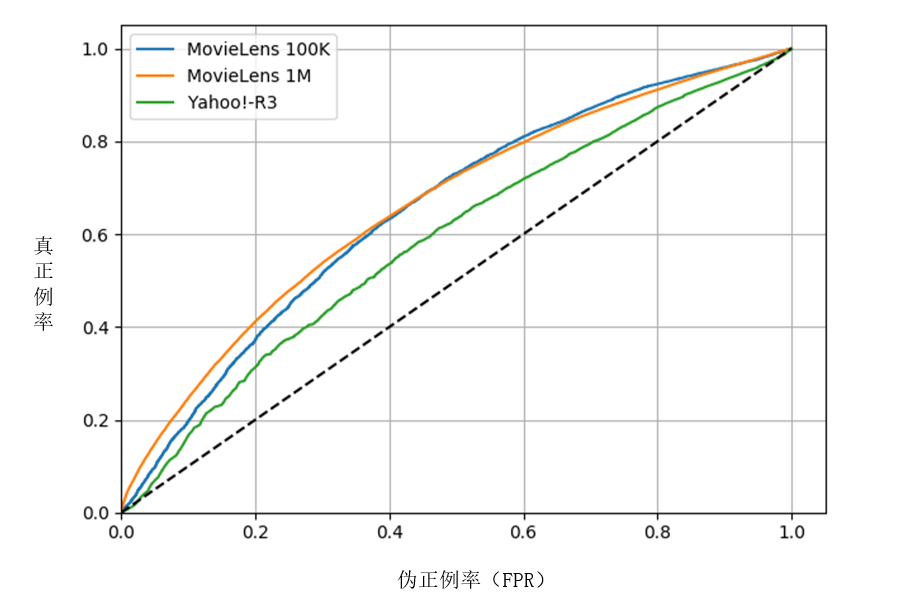
\includegraphics[width=0.7\textwidth]{2-roc.png}
	\caption{隐变量估计的ROC曲线}
	\label{Fig:ROC}
\end{figure}
\begin{table}[!]
	\centering
	\caption{隐变量的估计质量}\label{Table:ActionRecognition}
	\begin{tabular}{cccc}
		\toprule[1.2pt]
		数据集            & MovieLens-100k &	MovieLens-1M & Yahoo!-R3 \\ \hline
		AUC               & 0.6524       &  0.6618        & 0.5885 \\
		\bottomrule[1.2pt]
	\end{tabular}
\end{table}
图~\ref{Fig:ROC}绘制了通过不同估计阈值的所有交互的$\hat{c}_{ui}$的ROC(接收者操作特性)曲线,并且表~\ref{Table:ActionRecognition}计算了三个数据集对应的AUC。首先,$\hat{c}_{ui}$的AUC性能并不是很令人满意,但它们仍然比简单猜测抛硬币要好,显著大于50\%。这意味着,BPRAC算法总体上能够为偏好较高的交互输出一个较大的$\hat{c}_{ui}$估计值,为偏好较低的交互输出一个较小的$\hat{c}_{ui}$估计值。

为真实评分较高的物品输出一个较大的$\hat{c}_{ui}$预测值,使得模型从该物品学习更多信息;为真实评分较小的物品输出一个较小的$\hat{c}_{ui}$预测值,避免模型从噪声中学习到错误的信息,从而误判用户的兴趣偏好。在仅具有二元交互的有限信息下,$\hat{c}_{ui}$估计的有效性主要来自于次序统计量,它导致了后验分布的收窄,从而减小了随机变量的不确定性,如公式~\eqref{Eq:Bayesian}所描述。
\par 
\subsubsection{个性化推荐性能} 

表~\ref{Table:Recommendation}比较了五种成对学习排序模型的个性化性能。首先,BPRAC模型在所有评估指标中表现最好,这得益于隐变量的引入。在E步,由于BPRAC算法总体上能够为偏好较高的交互输出一个较大的$\hat{c}_{ui}$估计值,为偏好较低的交互输出一个较小的$\hat{c}_{ui}$估计值,使得模型从可靠的交互学到更多信息,且避免从噪声中学到错误信息,从而更准确地学习用户的偏好,产生更准确的预测。其次,此外,BPR表现不佳,该方法没有在隐式反馈数据中的去噪机制,每个交互都被认为是体现用户偏好的交互,这显然是不符合实际情况的。该消融实验结果表明噪声交互的存在对成对学习模型产生了不利影响,验证了在隐式反馈数据集中去噪的必要性。再次,DenoiseRec通过引入小损失的技巧来降低噪声,取得了次优的结果,这说明小损失技巧对于成对学习算法也是适用的;然而,与BPRAC相比,DenoiseRec收敛到一个较小的AUC值。在去噪机制方面,二者的唯一差异在于权重的计算机制不同:在BPRAC方法中,权重,即隐变量$\hat{c}_{ui}$是自适应学到的;而在DenoiseRec方法中,权重是手动设计的。手动设计权重依赖于密集的调参;另一方面,手动设计的权重通过下加权损失值较大的样本,削弱了困难负样本对学习算法的贡献。因为较大的损失值,可能是由于困难负样本所导致的。因此,自适应的参数学习比经验地手动设置权值更有效。

\begin{table*}[!]
	\centering
	\caption{Top-k 推荐性能比较}\label{Table:Recommendation}
	\resizebox{1\textwidth}{!}{
		\begin{tabular}{llccccccccccc}
			\toprule[1.2pt]
			\multirow{2}*{\textbf{数据集}} & \multirow{2}*{\textbf{方法}}  & \multicolumn{5}{c}{Top-5评估} &~& \multicolumn{5}{c}{Top-10评估}\\ \cline{3-7} \cline{9-13}
			~&~ & Precision & Recall & F1 & NDCG & MAP&~ & Precision & Recall & F1 & NDCG & MAP \\ \cline{1-7} \cline{9-13}
			\multirow{4}*{MovieLens-100K} & BPR & 0.2888 & 0.1897 & 0.1818 & 0.3401 &0.4893 &~  & 0.2379 & 0.2923 & 0.2075 & 0.3422 & 0.4663  \\
			~ & GBPR & 0.2976 & 0.1944 & 0.1872 & 0.3504 &0.4967&~ & 0.2458 & 0.3031 & 0.2147 & 0.3538 & 0.4780 \\
			~ & MPR & 0.1224 & 0.0741 & 0.0754 &0.1333& 0.2278&~ & 0.1053 & 0.1331 & 0.0935 & 0.1412 & 0.2295  \\
			~ & DenoiseRec & \underline{0.3042} & \underline{0.1990} & \underline{0.1883} &\underline{0.3528}&\underline{0.5122}&~ & \underline{0.2541} & \underline{0.3027} & \underline{0.2192} & \underline{0.3553} & \underline{0.4955}  \\
			~& \textbf{BPRAC} & \textbf{0.3265} & \textbf{0.2158} &\textbf{0.2055}  & \textbf{0.3879} &\textbf{0.5393} &~ & \textbf{0.2665} & \textbf{0.3216} &\textbf{0.2305} & \textbf{0.3859} &\textbf{0.5127}  \\ \cline{1-7} \cline{9-13}
			
			\multirow{4}*{MovieLens-1M} & BPR & 0.2940 & 0.1086 & 0.1323 & 0.3148 &0.4645&~ & 0.2570 & 0.1825 & 0.1741 & 0.3042 & 0.4517  \\
			~& GBPR & 0.3119 & 0.1265 & 0.1497 & 0.3376 &0.5004 &~ & 0.2655 & 0.2027 & 0.1874 & 0.3235 & 0.4797 \\
			~& MPR & 0.1125 & 0.0410 & 0.0494 & 0.1212 &0.2226&~ & 0.1036 & 0.0713 & 0.0681 & 0.1207 & 0.2278 \\
			~ & DenoiseRec & \underline{0.3205} & \underline{0.1174} & \underline{0.1434} &\underline{0.3432}&\underline{0.4996}&~ &\underline{0.2737}&\underline{0.1901} & \underline{0.1831} & \underline{0.3257} & \underline{0.4783}  \\
			~& \textbf{BPRAC} & \textbf{0.3472} & \textbf{0.1282} & \textbf{0.1572} & \textbf{0.3721} &\textbf{0.5297} &~ & \textbf{0.2992} & \textbf{0.2110} & \textbf{0.2026} & \textbf{0.3559} & \textbf{0.5044}  \\\cline{1-7} \cline{9-13}
			
			\multirow{4}*{Yahoo!-R3} & BPR & 0.0861 & 0.1007 & 0.0840 & 0.1099 & 0.1890 &~ & 0.0685 & 0.1566 & 0.0875 & 0.1284 & 0.1962  \\
			~ & GBPR & 0.1044 &0.1250 & 0.1037 & 0.1343 &0.2292&~ & 0.0817 &0.1943 & 0.1063 & 0.1576 & 0.2351  \\
			~ & MPR & 0.0694 & 0.0642 & 0.0511 & 0.0744 &0.1353&~ &0.0551 & 0.1095 & 0.0527 & 0.0875 & 0.1503  \\
			~ & DenoiseRec & \underline{0.1058} & \underline{0.1257} & \underline{0.1042}&\underline{0.1349}&\underline{0.2247}&~ & \underline{0.0841} & \underline{0.1993} & \underline{0.1086} & \underline{0.1596} & \underline{0.2326}  \\
			
			~& \textbf{BPRAC} & \textbf{0.1117} & \textbf{0.1308} & \textbf{0.1096} & \textbf{0.1448} &\textbf{0.2465}&~  & \textbf{0.0857} &\textbf{0.2034} & \textbf{0.1109} & \textbf{0.1675} & \textbf{0.2510} \\
			\bottomrule[1.2pt]
		\end{tabular}
	}
\end{table*}


\subsubsection{对噪声数据的敏感性}
图~\ref{Fig:impactd}展示了BPRAC算法对不同噪声率地敏感性。通过训练集中随机生成噪声数据,可以模拟训练集中含有更高噪声交互的情况。以噪声率控制数据集中噪声数据的比例,生成包含噪声的训练集时,不同的学习算法使用相同的含有噪声的训练集训练。对比方法选择BPR和DenoiseRec。如图~\ref{Fig:impactd}所示,噪声率的增加导致三种学习算法的个性化推荐性能都下降,表明噪声交互的存在对学习模型产生不利影响,且噪声率越高,对准确学习用户偏好的不利影响越大;另一方面,由于BPRAC和DenoiseRec包含去噪机制,它们相对于BPR更具鲁棒性。此外,DenoiseRec的性能下降略多于BPRAC,这意味着通过自适应地学习置信度,比经验地手动设定权重更加有效。
\begin{figure*}[!]
	\centering
	\subfloat{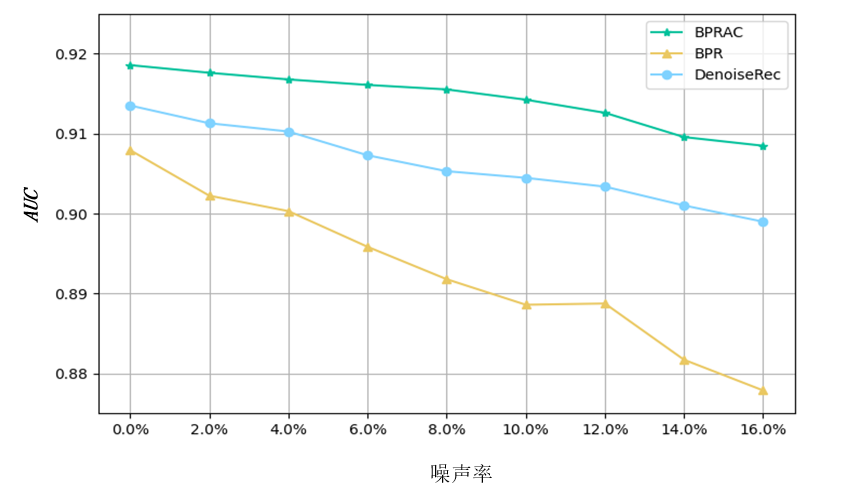
\includegraphics[width=.7\textwidth]{2-noisyratio.png}}
	\caption{不同噪声率对学习算法性能的影响}
	\label{Fig:impactd}
\end{figure*}
\par
\subsubsection{算法收敛性分析}
 图~\ref{Fig:Covergence}比较了五种算法的收敛性,度量指标为排序列表的AUC,这是因为成对损失函数可以类比于AUC指标\cite{Steffen:2009:UAI}。AUC指标的收敛意味着算法的收敛。首先观察到,所有算法的AUC在足够的训练迭代后首先增加,然后收敛。这个试验结果也印证了引理~\ref{Lemma:ConvergenceAnalysis}的分析,如公式~\eqref{Eq:PosteriorSupremum}所示。此外注意到,与对比算法相比,本章提出的的BPRAC收敛到一个更高的AUC指标,代价是更慢的收敛速率从而需要更多的训练轮次,通常需要比BPR多进行2-3倍更新,这是由于引入了新的隐藏变量$c_{ui}$。这个代价是值得的,因为BPRAC提供了一种从噪声数据中学习排序的解决方案。最后,专门针对噪声的DenoiseRec方法,由于引入了小损失技巧,把损失值较大的样本进行下加权,从而也降低了困难负样本对学习算法的贡献,因此也具有较慢的收敛速率,通常需要更多次的迭代。
\begin{figure}[!]
	\centering
	\subfloat{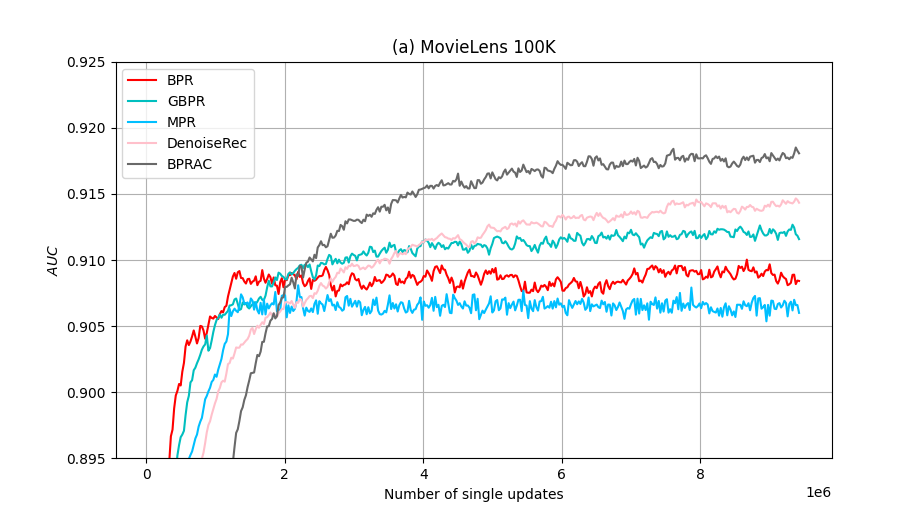
\includegraphics[width=.8\textwidth]{2-c100k.png}}\\
	\subfloat{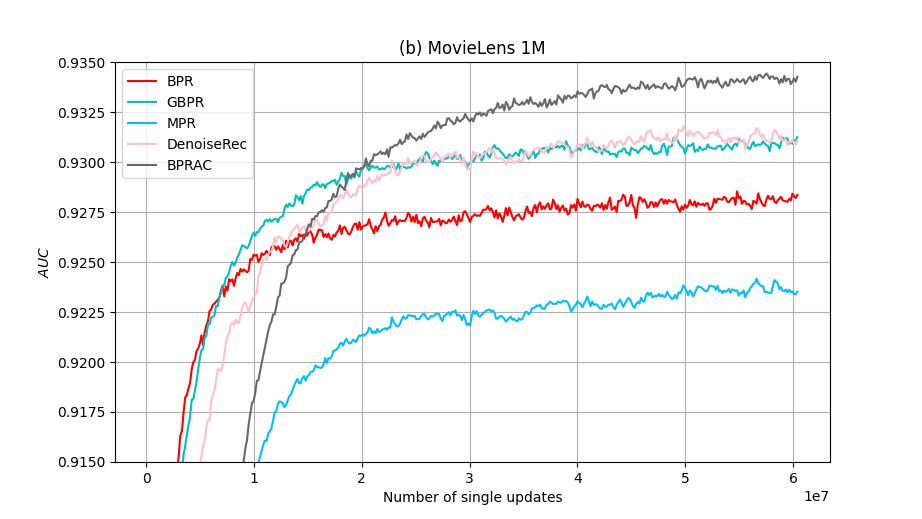
\includegraphics[width=.8\textwidth]{2-c1m.png}}\\
	\subfloat{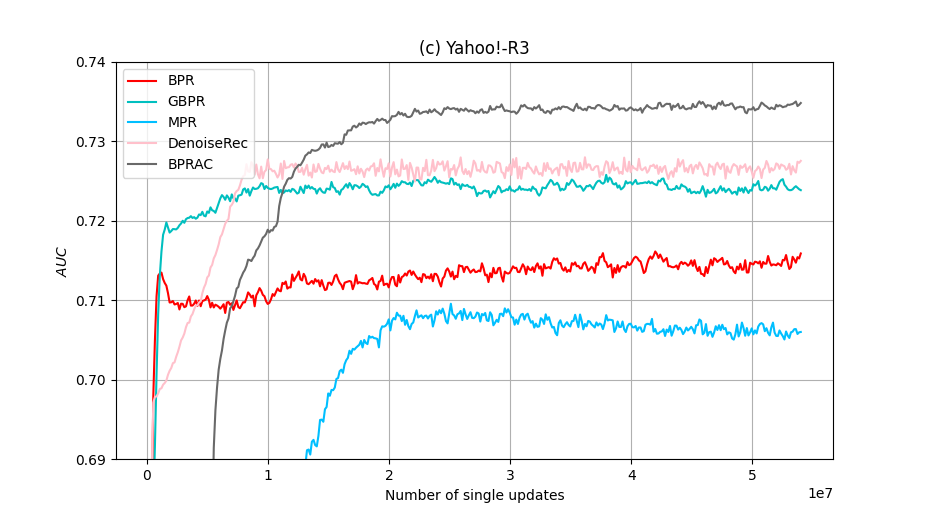
\includegraphics[width=.8\textwidth]{2-cyahoo.png}}
	\caption{不同学习算法的收敛速度比较}
	\label{Fig:Covergence}
\end{figure}

\section{本章小结}
本章聚焦于推荐系统的伪正例问题,研究了从含噪成对比较中学习排序的问题。由于隐式反馈是不完全数据,其中的伪正例构建的噪声成对比较,会对学习算法产生不利的影响。对于每个交互数据,本章引入了一个隐变量指示其可信度,并把从不完全数据中学习排序的问题形式化为一个含有隐变量的最大后验估计问题。针对这一问题,本章提出了自适应去噪的成对排序算法(BPRAC),端到端地估计隐变量并学习用户和物品表示。BPRAC算法在EM框架下求解:在E步固定模型参数估计隐变量,在M步固定隐变量学习模型参数。对真实的推荐数据集进行的实验BPRAC算法相对于其他对比方法的优越性。但是,相对于异常交互模式产生的伪正例问题,负例未标是隐式反馈数据面临的一个更突出问题,也是机器学习更具普遍性的问题。本章的研究将为后续章节中探索更复杂模型和更一般的伪负例场景的解决方案提供启示。
\chapter{负例采样算法研究}
\label{cha:thirdsection}
本章聚焦推荐系统中的伪负例问题。隐式反馈数据面临的一个突出问题是负例未标注。通常,未交互的物品被当作负样本以训练模型。然而,其中存在没曝光给用户,但是用户可能喜欢的物品,从而导致了伪负例问题。这一问题在自监督学习的诸多领域具有普遍性,例如在自然语言处理(NLP)中,正样本可以从上下文中获得,而负样本则是从未标注的词库中随机抽样得到的。在计算机视觉(CV)中,正样本通过数据增强获得,而负样本则从未标记的图像中抽样得到。这样的数据集也被称为Positive-Unlabeled (PU)数据集。如何从未标记的数据中采样高质量的负实例,即负采样,对于训练基于对比学习的模型非常重要。本章聚焦于推荐系统中负采样问题的研究,通过设计最优负采样准则,采样信息量大且用户不喜欢的硬负样本(hard negative),以提升推荐精度。
\begin{figure*}[h!]
	\centering
	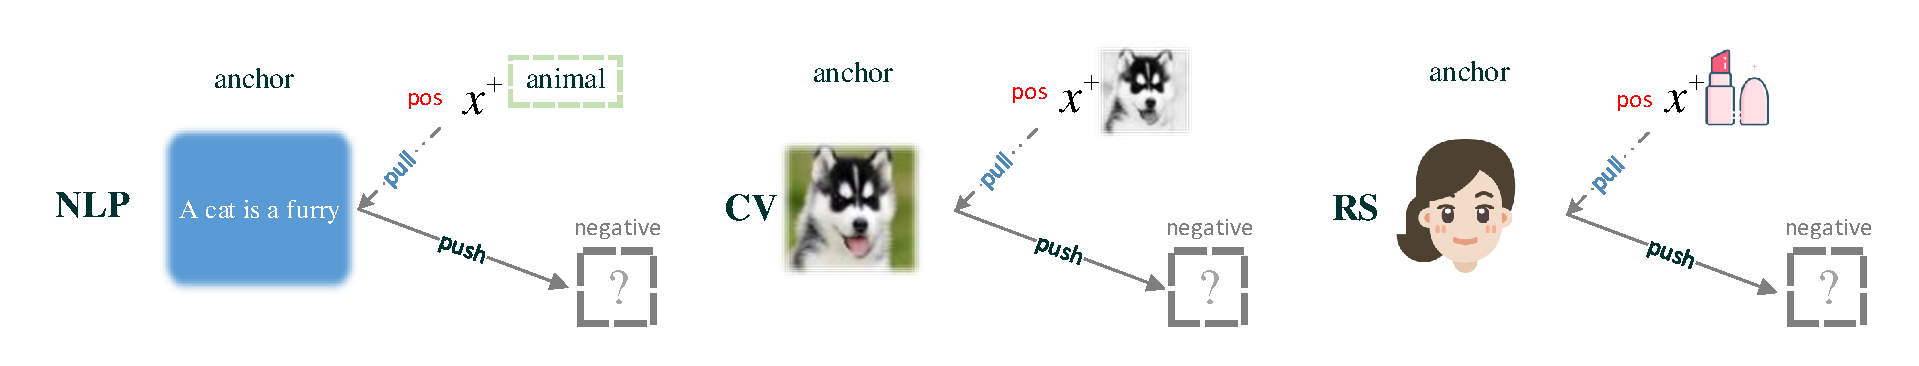
\includegraphics[width=\textwidth]{3-PU.pdf}
	\caption{Positive-Unlabeled(PU)问题示意图}
	\label{Fig:falsen}
\end{figure*}
\section{引言}
负采样源自Positive-Unlabeled (PU)问题~\cite{Jessa:2020:ML,Su:2021:IJCAI}。一个典型的PU数据集,通常只有部分正例被标注,其余样本未标注,而这些未标注的样本可能属于正类或负类。负采样,即确定从PU数据集中采样负例的策略,以便有效地训练下游任务模型。负采样在许多任务中都有广泛应用,例如自然语言处理(NLP)\cite{Mikolov:2013:NIPS,Tang:2015:WWW},计算机视觉(CV)\cite{Qin:2021:AAAI,Zhao:2021:IJCAI},以及推荐系统(RS)~\cite{Steffen:2014:WSDM,Zhang:2013:SIGIR,Ding:2020:NIPS}。本章聚焦于推荐系统中的负采样。对于一个特定的用户,他未交互的物品,称为他的\textit{负例}。里面包含用户确实不喜欢的物品,称为\textbf{真负例};也包含用户喜欢的物品,称之为\textbf{伪负例}(即正例)。负采样的困境在于,未标注的样本中含有用户潜在喜欢的伪负例,一旦这类用户感兴趣的样本被采样当作负例用于训练模型,会使得模型误判用户的兴趣边界。这激发了负采样用于推荐的问题,即如何有效地采样负实例来训练推荐模型。许多研究表明,负采样对于提高推荐性能非常重要~\cite{Steffen:2014:WSDM,Zhang:2013:SIGIR,Ding:2020:NIPS,Park:2019:WWW,Huang:2021:KDD,Ding:2019:IJCAI,Yang:2020:KDD}。

负采样算法在推荐系统中被广泛研究。根据抽样分布是否随模型状态的变化,可以将现有的负采样算法分为以下两类:\textit{静态负采样}\cite{Steffen:2009:UAI,Chen:2017:KDD,Mikolov:2013:NIPS,Xiangnan:2020:SIGIR,Weike:2013:IJCAI,Yu:2018:CIKM,Wang:2019:SIGIR}。这类算法根据固定的采样分布,如均匀采样,依物品流行度的采样等,这类抽样分布所参照的信息是静态的,不随模型训练的参数变化而变化。另外一类是\textit{动态负采样}\cite{Steffen:2014:WSDM,Zhang:2013:SIGIR,Wang:2020:WWW,Chen:2019:WWW}。这类负采样算法的抽样分布会根据模型训练不断调整,偏好于采样在嵌入空间中与正例表示更相似的负例,即难以区分的困难样本(hard negative sample),例如采样分数更高或排名更高的实例~\cite{Steffen:2014:WSDM,Zhang:2013:SIGIR,Zhao:2015:CIKM}。静态负采样可以使用某些辅助信息,免于采样到用户感兴趣的伪负例。但是由于其抽样分布是静态的,往往只会采样容易样本,不利于模型性能的提升;动态负采样可以根据模型的训练针对困难样本进行采样,更容易受到负采样问题的困扰~\cite{Ding:2020:NIPS,Qin:2021:AAAI,Zhao:2021:IJCAI}。

本章对推荐系统的负采样研究做出了以下三个方面的贡献:(1) 根据经验分布函数的渐近性质,定义了一个与模型无关的负信号测度,用于度量未标注样本是真负例的后验概率。特别地,它较好地结合了现有基于先验信息(与模型无关)以及基于样本信息(与模型相关)的两种提取负信号的范式。 (2) 本章还提出了最优采样准则,用于采样高质量的负例。这是一个经验采样风险最小化的理论最优采样准则。实验证明了所提出的负采样算法在采样质量和推荐性能方面的有效性。

\section{负采样分析}
对于一个由$M$个用户和$N$个物品组成用户-物品交互矩阵$\mathbf{X}=[x_{ui}] \in \mathbb{R}^{M\times N}$,元素$x_{ui}=1$表示用户$u$与物品$i$有交互;否则,$x_{ui}=0$。为了训练推荐模型 $\mathcal{M}$,我们考虑如下广泛使用的BPR优化目标:
\begin{equation}\label{Eq:PairewiseLossFunction}\
	\mathcal{L} = \sum_{(u,i,j)} \ln \sigma(\hat{x}_{ui} - \hat{x}_{uj}) ,
\end{equation}
对于用户 $u$,其中 $\hat{x}_{ui}$ 和 $\hat{x}_{uj}$ 分别是他已交互物品 $i$ 和未交互物品 $j$ 的预测分数,由用户物品表示$\Theta$参数化:$\hat{x}_{ui} = \mathtt{sim}(\mathbf{w}_u, \mathbf{h}_i)$,其中 $\mathtt{sim}$ 是相似度函数,例如余弦相似度或点积函数。$(u,i,j)$为训练三元组。训练三元组 $(u,i,j)$ 的构建如下:对于用户 $u$ 和他的一个正例 $i \in \mathcal{I}_u^+$,负例从未标注样本中随机采样一个 $j \in \mathcal{I}_u^-$,即进行负采样。存在着两种情况,即用户 $u$ 实际上喜欢$j$,未交互仅仅是因为之前没有看到过它,也就是说,物品 $j$ 对于用户 $u$ 来说是一个伪负例。另一方面,如果用户 $u$ 确实不喜欢物品 $j$,则该物品被称为真负例。

\par
通常使用\textit{随机梯度下降}(SGD)来迭代优化每个训练三元组 $(u, i, j)$ 的损失函数。对于采样的实例 $j \in \mathcal{I}_u^-$,如果它是用户 $u$ 的真负例,则相对于其预测得分 $\hat{x}_{uj}$ 的损失梯度计算如下
\begin{equation}\label{Eq:GradientOriginal}
	\frac{\partial \mathcal{L} }{\partial \hat{x}_{uj}} = [1-\sigma(\hat{x}_{ui} - \hat{x}_{uj})] (-1),
\end{equation}
其中 $\sigma(\cdot)$ 是 \textsf{sigmoid} 函数。然而,如果采样的实例 $j$ 实际上是一个伪负例,根据微分的链式法则,正确的梯度更新应该是相反,即公式~\eqref{Eq:GradientOriginal}的最后一项 $(-1)$改为$(+1)$。由此可见,对于一个未标注样本,由于其标签不同,梯度方向也截然相反。因此可以把损失函数相对于未标注样本地损失梯度写为:
\begin{equation}\label{Eq:Gradient}
	\frac{\partial \mathcal{L}_{loss} }{\partial \hat{x}_{uj}} = [1-\sigma(\hat{x}_{ui} - \hat{x}_{uj})] \cdot \mathtt{sgn}(j),
\end{equation}
其中,如果 $j$ 是用户 $u$ 的真负例,则 $\mathtt{sgn}(j)=-1$;如果 $j$ 是用户 $u$ 的误判负例,则 $\mathtt{sgn}(j)=1$。损失函数的梯度公式~\eqref{Eq:Gradient} 可以分解为两部分,即\textit{梯度幅度}和\textit{梯度方向}。这激发了我们对负采样的分析,即什么是高质量的负例:如果在训练三元组 $(u,i,j)$ 中采样的实例 $j$ 同时具有信息量和无偏性,那么它被称为\textit{高质量负例}。
\begin{itemize}
	\item \textbf{信息量}: 未标注样本$j$的信息量定义为该样本对应的损失函数梯度幅度的大小,即
	\begin{equation}\label{Eq:Informativeness}
		\mathtt{info}(j) =  [1-\sigma(\hat{x}_{ui} - \hat{x}_{uj})].
	\end{equation}
	\item \textbf{无偏性}: 未标注样本$j$的信息量定义为该样本是真负例的后验概率大小,即
	\begin{equation}\label{Eq:Unbiasedness}
		\mathtt{unbias}(j) = \mathrm{P}(\mathtt{sgn}(j) = -1).
	\end{equation}
\end{itemize}

信息量与未标注样本$j$ 对于推荐模型参数更新的帮助程度相关。给定正例的预测得分 $\hat{x}_{ui}$,如果未标注样本$\hat{x}_{uj}$ 的值过小,则 $\sigma(\hat{x}_{ui} - \hat{x}_{uj}) \rightarrow 1$ 且 $\mathtt{info}(j) \rightarrow 0$,即梯度消失,无法从未标注样本$j$上学到太多信息。这是困难负采样(hard negative sampling)的一个重要动机。

无偏性实际上定义为未标注样本$j$ 是真负例的概率。对于负采样而言,正例已经给定,目标是采样真负例。在训练时,把采样到的未标注样本当作负例,即直接设置 $\mathtt{sgn}(j)=-1$。当存在采样偏差时,即采样到正例,将导致推荐模型误判用户的兴趣边界。如何从未标记的样本中识别出真负例示例是必须解决的负采样关键研究问题。

采样偏差的不良影响不仅限于BPR损失,上述分析可以同样推广到其他一些基于对比的损失函数如InfoNCE,也可能因错误的负采样而受到影响:当采样一个伪负例时,损失函数对于该采样的样本梯度方向错误。这个伪负例的特征表示将被推离锚点$u$,而实际上它应该在嵌入空间中靠近锚点。

\section{贝叶斯最优负采样算法}
\subsection{类条件概率密度} \label{Sec:Dis}
由于所有未标注样本的预测得分都是使用相同的编码器和相同的得分函数预测的,因此可以假设预测得分 $\hat{x}$ 是独立同分布的,其概率密度函数记为抽象函数$f(\hat{x})$,相应的累积分布函数为 $F(\hat{x}) =\int_{- \infty }^{\hat{x}} f(t)dt$。

考虑未标注样本中的两个总体:真负例和伪负例。根据成对学习的优化目标,是针对锚点和正例的相似度分数高于负例的相似度分数进行优化。这表明以下预测得分的次序关系可能在一般情况下成立
\begin{equation}\label{Eq:OrderRelation}
	X_{tn} \leq X_{fn},
\end{equation}
其中,$X_{tn}$ 和 $X_{fn}$ 分别为真负例和伪负例(即未来测试数据中的正例)的预测得分的随机变量。需要注意的是,这也是对比学习方法~\cite{gutmann:2012:JMLR,Oord:2018:arxiv,Gutmann:2010:ICAIS} 的优化目标,其本质上鼓励学到的正例特征表示与“锚点”数据点相似,同时将负例特征与“锚点”数据在嵌入空间中推远,使其不相似\cite{Wang:2020:ICML,Xu:2022:arxiv,Liu:2021:TKDE}。

真负例和伪负例两个总体预测分数的这种序关系,可以使用次序统计量的技术写出真负例和伪负例这两个总体相似度分数分布:
\begin{eqnarray}\label{Eq:TNpdf}
g(\hat{x}_{tn}) &=& 2 f(\hat{x}_{tn}) [1 - F(\hat{x}_{tn})],\\
h(\hat{x}_{fn}) &=& 2 F(\hat{x}_{fn}) f(\hat{x}_{fn}).	
\end{eqnarray}
\subsubsection{经验分布}\label{Appendix:Realdist}
为了验证公式~\eqref{Eq:OrderRelation} 的次序关系,在模型训练过程中记录真负例总体(TN)和伪负例总体(FN)相似度分数的经验分布。其中,伪负例总体是测试集中的物品,在训练过程中无法观测;真负例总体是未交互物品中,除去测试集之外的其余物品。在MovieLens-100K数据集上,采用经典的矩阵分解推荐模型,并采用随机负采样在训练集上训练模型,并记录每个训练周期的预测得分。通过统计真负例和误判负例的预测得分,在图~\ref{Fig:DistributionStatistics} 中报告了它们在模型训练中的分布密度。
\begin{figure*}[h!]
	\centering
	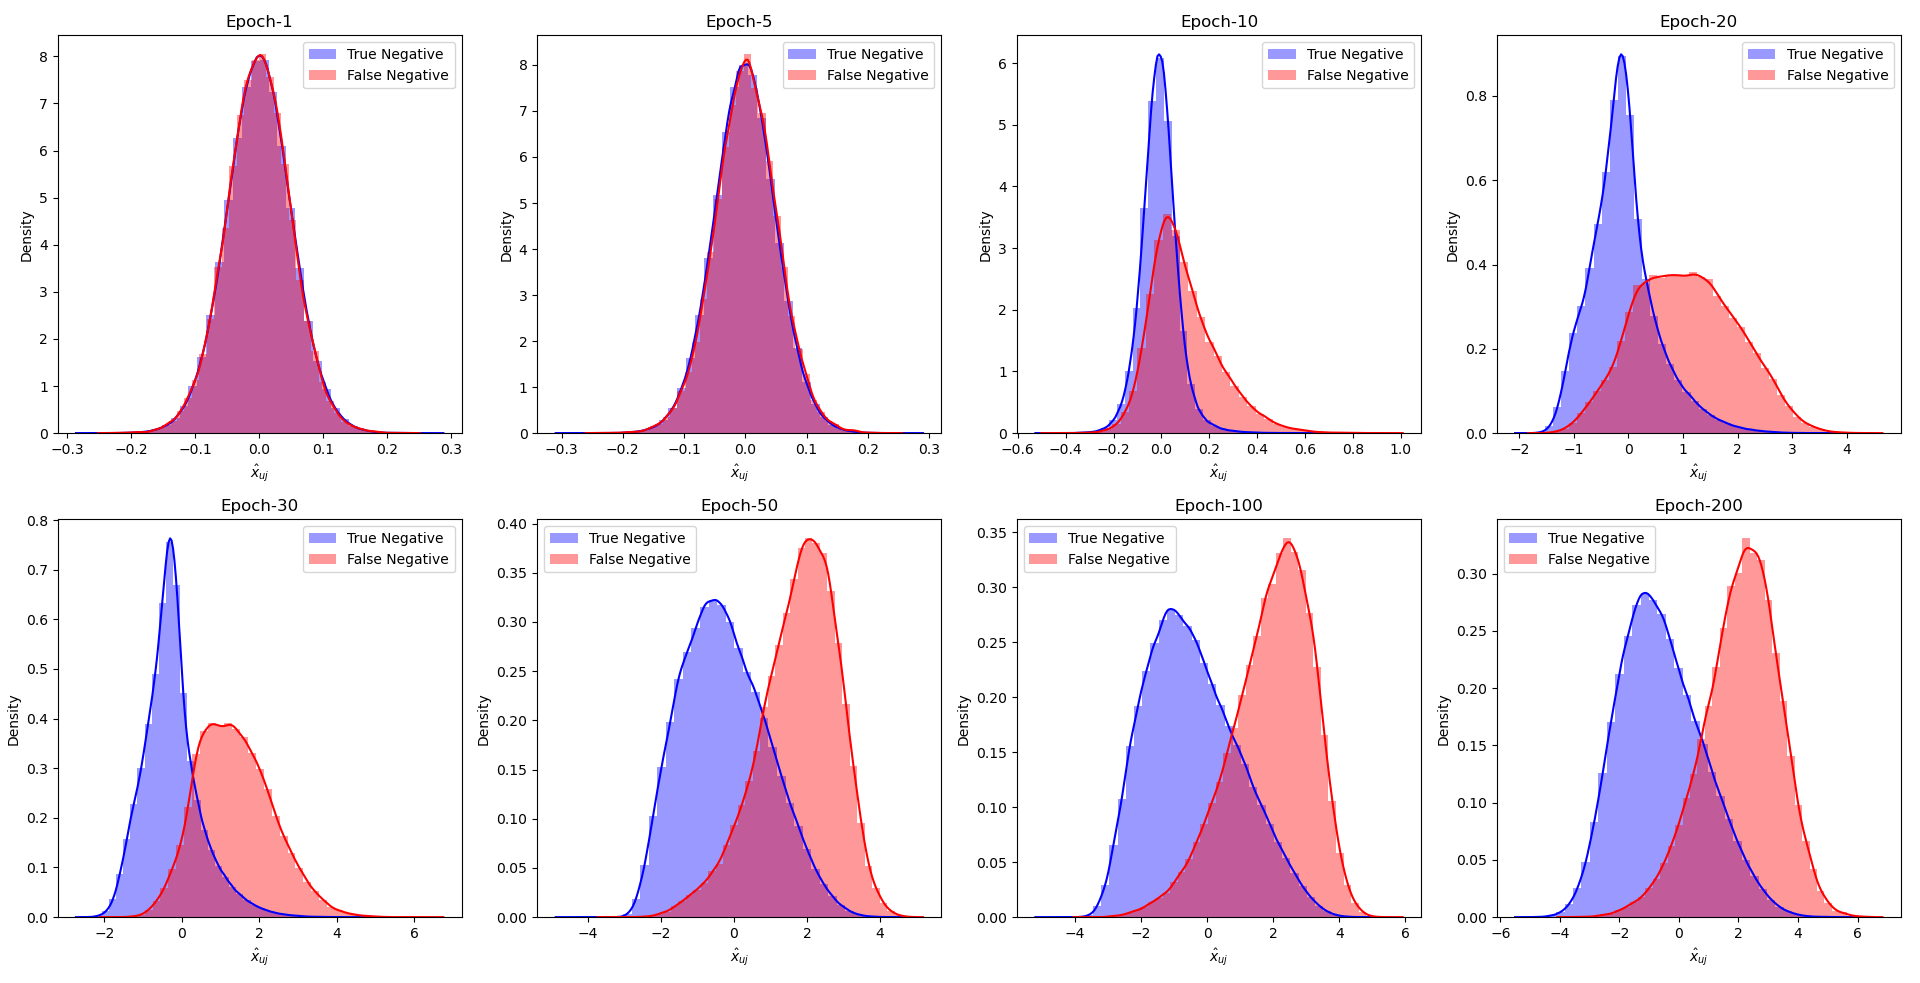
\includegraphics[width=\textwidth, height=0.5\textwidth]{3-DistributionStatistics1.png}
	\caption{不同训练时点的相似度分数的经验分布}
	\label{Fig:DistributionStatistics}
\end{figure*}
\par
图~\ref{Fig:DistributionStatistics} 提供了两个发现:
\begin{itemize}
\item 负例的预测得分越高,它是伪负例的概率密度就越高,而是真负例的概率密度就越低;
\item 随着训练的进行,两个分布之间的区别逐渐变得更加清晰:与真负例相比,伪负例的分布集中在更高的得分上。这表明,相对于真负例而言,推荐模型总体上能够给伪负例更高的评分。
\end{itemize}

\subsubsection{理论分布}\label{Appendix:Theodist}
\begin{figure}[h!]
	\centering
	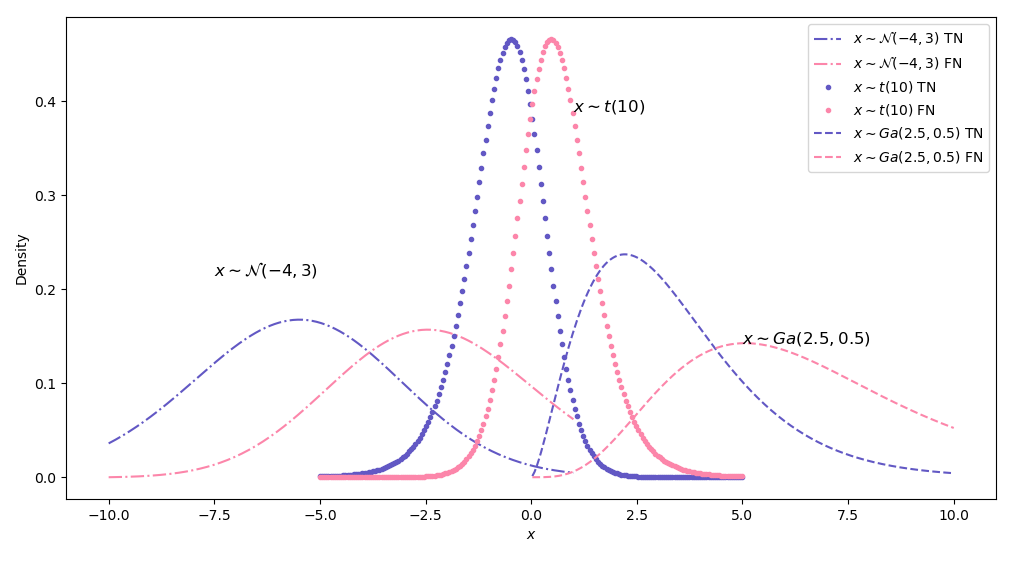
\includegraphics[width=.9\textwidth, height=0.45\textwidth]{3-theorydist.png}
	\caption{相似度分数的理论分布}
	\label{Fig:TheoryDist}
\end{figure}
图~\ref{Fig:TheoryDist} 展示了基于不同类型的分布$f(x)$时(高斯分布 $x\sim \mathcal{N}(\mu,\sigma)$,学生分布 $x\sim t(n)$ 和伽玛分布 $x\sim Ga(\alpha,\lambda)$),公式\eqref{Eq:TNpdf}所对应的真负例和伪负例的分数分布形态。在训练过程中,使用真实数据集绘制的经验分布图~\ref{Fig:DistributionStatistics},逐渐展示出了与图~\ref{Fig:TheoryDist} 中描述的理论分布出现了相同结构。

目前为止,我们还不知道 $f(x)$ 和 $F(x)$ 的显式表达式。不同的得分函数和推荐模型会产生不同的未标注样本分数密度表达 $f(\cdot)$,但这种分离的结构足以让我们对真负例和伪负例进行分类。此外,经验分布函数 $\hat F(x)= \frac{1}{n}\sum_j I_{|X_\cdot \leq \hat{x}_l|}$ 的计算很容易实现。 根据Glivenko定理~\cite{glivenko:1933},经验分布函数一致收敛于分布函数,使得可以通过计算经验分布函数,以实现对抽象函数$F(\cdot)$的近似。这一有力工具,使得本章所提出的负采样方法不再局限于简单的矩阵分解模型,可以向任何深度神经网络模型推广。

\subsection{贝叶斯分类}
对于一个未交互的物品$l$以及其对应的预测得分为$\hat{x}_l$,使用贝叶斯公式计算物品$l$为真负例的后验概率:
\begin{eqnarray} \label{Eq:PostTN}
	P(tn|\hat{x}_l) &\propto& P(\hat{x}_l|tn) P_{tn}(l) \nonumber \\
	&=&  2f(\hat{x}_l) [1 - F(\hat{x}_l)] P_{tn}(l),
\end{eqnarray}
其中,$P(\hat{x}l|tn)$ 是真负例的类条件密度,由 $g(\hat{x})$ 给出;$P_{tn}(l) = 1 - P_{fn}(l)$ 是物品 $l$ 为真负例的先验概率。$f(\hat{x}_l)$ 是所有未标注样本的得分分布,$F(\hat{x}_l) = \int_{-\infty}^{\hat{x}_l} f(t) dt$ 是相应的累积分布函数。同样地,未标注样本$l$是伪负例的后验概率为
\begin{eqnarray}\label{Eq:PostFN}
	P(fn|\hat{x}_l) &\propto& P(\hat{x}_l|fn) P_{fn}(l) \nonumber \\
	&=& 2 F(\hat{x}_l) f(\hat{x}_l) P_{fn}(l)
\end{eqnarray}

贝叶斯分类器可以通过最大化后验概率来得到:
\begin{eqnarray}
	\mathop{\arg\max}\limits_{c \in \{fn, tn\}} P(c|\hat{x}_l).
\end{eqnarray}

直接计算公式~\eqref{Eq:PostTN} 和公式~\eqref{Eq:PostFN} 中的得分密度函数 $f(\cdot)$ 并不实际。然而,计算经验分布函数却很容易实现。因此,使用贝叶斯公式的分式形式定义无偏性,以消除密度函数 $f(\cdot)$:
\begin{eqnarray}
	\mathtt{unbias}(l) &\triangleq&  P(tn|\hat{x}_l) = \frac{P(tn,\hat{x}_l)}{P(\hat{x}_l)} \label{Eq:NorPost} \\
	&=& \frac{P(\hat{x}_l |tn)P_{tn}(l)}{P(\hat{x}_l |tn)P_{tn}(l)+P(\hat{x}_l |fn)P_{fn}(l)} \\
	&=& \frac{ f(\hat{x}_l) [1 - F(\hat{x}_l)] P_{tn}(l)}{ f(\hat{x}_l) [1 - F(\hat{x}_l)] P_{tn}(l) + F(\hat{x}_l) f(\hat{x}_l) P_{fn}(l) }  \nonumber\\
	&=&  \frac{  [1 - F(\hat{x}_l)][1-P_{fn}(l)] }{1 - F(\hat{x}_l) -P_{fn}(l) + 2F(\hat{x}_l)P_{fn}(l) }.\label{Eq:unbias}
\end{eqnarray}
根据 Glivenko 定理~\cite{glivenko:1933},可以使用 $\hat F(\hat{x}_l)$ 来近似 $F(\hat{x})$,即 $\hat{x}_{\cdot} \leq \hat{x}_l$的比例:
\begin{eqnarray}\label{Eq:CDF}
 F(x) \simeq \frac{1}{n}\sum_j I_{|X_\cdot \leq \hat{x}_l|}
\end{eqnarray}
$P_{fn}(l)$ 是物品 $l$ 为伪负例的先验概率。假设物品 $l$ 被交互的次数 $pop_l \sim B(N, P_{fn}(l))$,其中 $N$ 是训练集中的总交互次数。那么,
\begin{eqnarray}\label{Eq:Prior}	
	P_{fn}(l) = \frac{pop_l}{N}.
\end{eqnarray}

%\begin{lemma}[Unbiased negative signal]\label{unbias}
%	If $pop_l \sim B (N, P_{fn}(l))$, then $\mathtt{unbias}(l)$ measure given by Eq~\eqref{Eq:unbias} is an unbiased estimator for $l$ being true negative.
%	
%	\begin{proof}
%		Setting random variable $Y=1$ if $l \in fn$, otherwise $Y=0$,
%		\begin{eqnarray}
%			Y= \left\{
%			\begin{aligned}
%				1 ,~ P &=& \theta \\
%				0 ,~ P &=& 1-\theta, \\
%			\end{aligned}
%			\right.
%		\end{eqnarray}
%		where $\theta$ is the probability of $l$ being false negative. So $Y \sim B(1,\theta)$. $pop_l = Y_1 + Y_2 + \cdots + Y_N  \sim B(N,\theta)$, then $P(pop_l=k )= \binom{N}{k} \theta^k (1-\theta)^{(N-k)} $. So
%		
%		\begin{eqnarray}
%			\mathbb{E}[P_{fn}(l)] &=& \mathbb{E}(\frac{pop_l}{N}) \nonumber \\
%			&=& \theta
%		\end{eqnarray}
%		
%		Given the observation $ X = \hat{x}_{ul}$, $F(X)$ is a statistic of $X$. $P_{fn}(l)$ is a statistic of $\sum_i Y_i$ that is independent of $X$. So
%		\begin{eqnarray}
%			&&\mathbb{E} [\mathtt{unbias}(l)]  \nonumber \\
%			&=& \mathbb{E}   \frac{  [1 - F(X)][1-P_{fn}(l)] }{1 - F(X) -P_{fn}(l) + 2F(X)P_{fn}(l) } \nonumber  \\
%			&=&  \frac{  [1 - \mathbb{E}  [F(X)]] [1- \mathbb{E} [ P_{fn}(l)]] }{1 -\mathbb{E} [F(X)] - \mathbb{E}[P_{fn}(l)] + \mathbb{E} [2F(X)P_{fn}(l)] }
%		\end{eqnarray}
%		$\mathbb{E}[F(X)]$ is the first order origin moment of cumulative distribution function $F(X)$
%		\begin{eqnarray}
%			\mathbb{E}  [F(X)] &=& \int_{-\infty}^{\infty} F(x) f(x) dx\nonumber\\
%			&= &  \int_{-\infty}^{\infty} F(x) dF(x)\nonumber\\
%			&= &  \frac{1}{2}  F^2(x)   \bigg|_{x=-\infty}  ^{x=\infty} \nonumber\\
%			&= & \frac{1}{2}.
%		\end{eqnarray}
%		So
%		\begin{eqnarray}
%			\mathbb{E} [\mathtt{unbias}(l)] &=&  \frac{  (1 - \frac{1}{2}) (1-\theta) }{1 -\frac{1}{2} - \theta + 2\cdot \frac{1}{2} \cdot \theta} \nonumber  \\
%			&=& 1-\theta.
%		\end{eqnarray}
%		Note $1-\theta$ is the probability of $Y=0$ from binomial populations $Y\sim B(1,\theta)$, so $\mathtt{unbias}(l)$ is unbiased estimator of $l$ being true negative. Fig~\ref{Fig:unbias} plots $\mathtt{unbias}(l)$ as a function of $F(\hat{x}) \in [0,1]$ and $P_{fn}(l) \in [0,1]$. We observe that $\mathtt{unbias}(l)$ is a decreasing function w.r.t both $F(\hat{x})$ and $P(fn)$. The monotonicity of $\mathtt{unbias}(j)$ is consistent with our analysis, and the value domain of $\mathtt{unbias}(j)$ $\in [0,1]$ conforms to the probability form.
%		\begin{figure}[h]
%			\centering
%			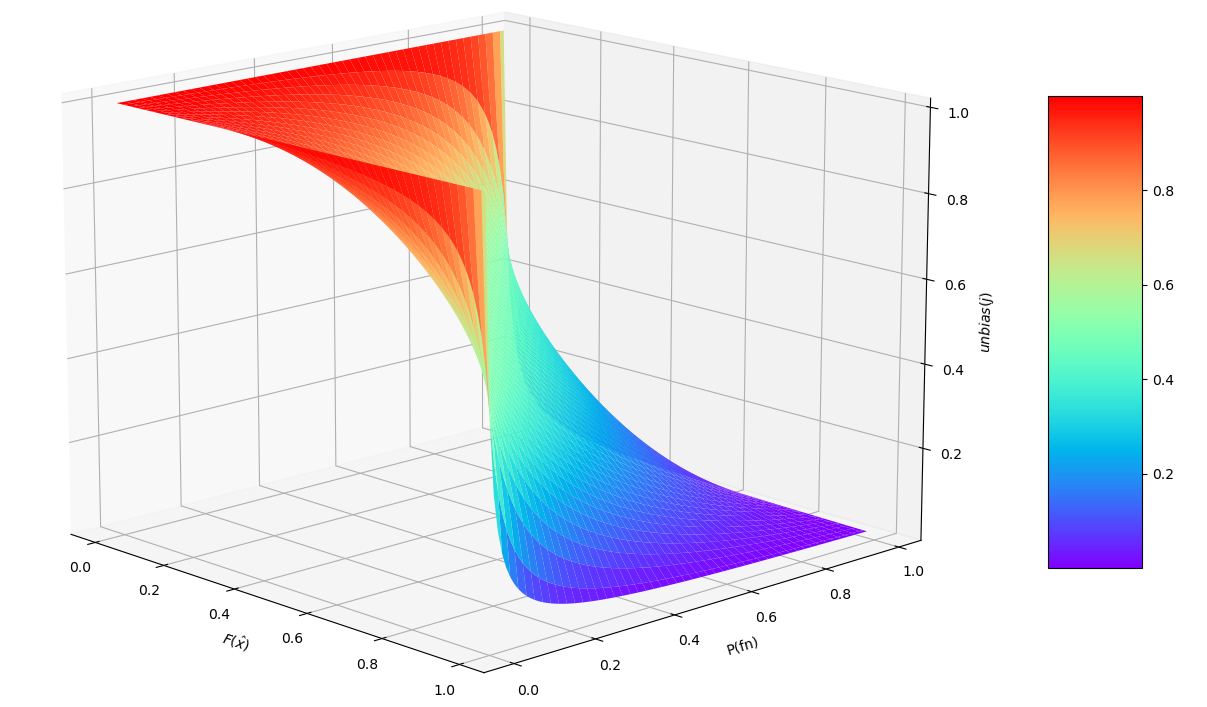
\includegraphics[width=0.4\textwidth]{3-unbias.png}
%			\caption{Numerical plots of posterior probability $\mathtt{unbias}(j)$ by Eq.~\eqref{Eq:unbias}.}
%			\label{Fig:unbias}
%		\end{figure}
%	\end{proof}
%\end{lemma}

无偏性的定义是物品$l$ 为真负例的后验概率。由于公式~\eqref{Eq:unbias}的分数表达式,未标注样本分数的密度函数 $f(\hat{x}_l)$ 被消除掉。公式~\eqref{Eq:unbias} 意味着未交互物品 $l$ 的负信号形式上由以下因素决定:(i) 推荐模型输出的排序位置,用 $F(\hat{x}_l)$ 表示,其中排序位置和 $F(\hat{x}_l)$ 具有一一映射关系。较大的 $F(\hat{x}_l)$,即靠前的的排序位置,表明推荐模型在很大程度上将 $l$ 分类为用户感兴趣的伪负例(正例),即$F(\hat{x}_l)$ 分配了一个在 $[0,1]$ 范围内的$l$ 是伪负例(正例)的概率预测。这解释了为什么那些过采样得分较高或排名较高的困难负例的算法~\cite{Steffen:2014:WSDM,Zhang:2013:SIGIR} 更容易采样伪负例的问题。(ii)先验信息,表示为先验概率($P_{tn}(l)$ 或 $P_{fn}(l)$)。

注意到,公式~\eqref{Eq:unbias} 的度量标准统一了当前关于提取负信号的两种主要范式:(i)建模先验信息,如 曝光数据~\cite{Jingtao:2019:IJCAI}、知识图谱实体~\cite{Wang:2020:WWW}、社交网络中的连接~\cite{Zhao:2014:CIKM,Wang:2016:CIKM} 等;(ii) 建依赖模型的样本信息,如预测得分~\cite{Steffen:2014:WSDM}、排名位置~\cite{Zhang:2013:SIGIR}、得分方差~\cite{Ding:2020:NIPS} 等。前者可以融入领域知识,但负信号与模型状态无关;后者利用样本信息 $\hat{x}_l$,但忽略了先验信息。$\mathtt{unbias}(\cdot)$ 测度的优势在于其对应的后验概率的理论解释:它结合了先验信息(与模型无关)和样本信息 $\hat{x}_l$(与模型相关)。本章只是为了简化,采用了一种简单的方法来建模先验概率,但不局限于此,$P_{tn}(l)$为使用其他附加信息和领域知识来建模先验概率提供了灵活的接口。

\subsection{最优采样准则}
公式~\eqref{Eq:PairewiseLossFunction}的成对损失$\mathcal{L}$ 可以类比于$AUC$ 指标~\cite{Steffen:2009:UAI}。它用可微的损失函数 $\ln \sigma(\cdot)$ 替代了 $AUC$ 指标中的不可微的0-1损失,这在优化 $AUC$ 时是一种常见做法~\cite{Herschtal:2004:ICML,Steffen:2009:UAI},因此关心$\mathcal{L}$的大小也是关心AUC指标的大小。

先在给定正例对$(u,i)$,采样到的样本$l$ 直接被赋予一个负向的梯度,导致预测得分 $\hat{x}_{ul}$ 的减少,这会对 $\mathcal{L}$ 产生两种影响:(i)当$l$是伪负例时,$\mathcal{L}$会减少,表示为 $\triangle \mathcal{L}_{fn}(l|i)$;(ii) 当$l$是真负例时,$\mathcal{L}$会增加,表示为 $\triangle \mathcal{L}_{tn}(l|i)$。

\begin{definition}[条件采样风险]
对于给定的正例对$(u,i)$,定义采样未标注样本$l$ 的条件采样风险为,采样损失$\triangle \mathcal{L}(l|i)$相对于$l$的标签$c$的期望值:
	\begin{eqnarray}
		R(l|i) 
		&=&  \mathbb{E}_{l \sim P(c|l)}  \triangle \mathcal{L}(l|i)\nonumber\\
		&=&[1- P(tn|l)] \cdot \triangle \mathcal{L}_{fn}(l|i) + P(tn|l)\cdot \triangle \mathcal{L}_{tn}(l|i)\label{eq:condirisk},
	\end{eqnarray}
其中$P(tn|l)$是$l\in tn$的后验概率,可以使用$\mathtt{unbias}(l)$计算, $ 1 - P(tn|l)$是$l\in fn$的后验概率。条件采样风险的的含义是,给定正例$i$,采样$l$所带来的AUC的期望减小值。
\end{definition}

\begin{definition}[经验采样风险]
采样器 $h$ 的经验采样风险为,条件采样风险$R(l|i)$对所有正例分布的期望值:
	\begin{eqnarray}
		R(h) = \mathbb{E}_{i \sim P(i)} R(l|i).
	\end{eqnarray}
经验采样风险的含义为,对于所有正例,采样器所带来的AUC的期望减小值。
\end{definition}
任务是找到一个采样策略 $h:\mathcal{I}_u^- \rightarrow l$,以最小化经验采样风险,从而实现最大化AUC。如下定理给出了经验采样风险最小化意义的最优采样准则:
\begin{theorem}[最优采样准则] \label{optimalrule}
若条件采样风险$R(l|i)$相互独立, 那么对任意采样器$h: \mathcal{I}_u^- \rightarrow l$,
	\begin{eqnarray}\label{Eq:OptimalSam}
		h^* &=&   \mathop{\arg\min}\limits_{l \in\mathcal{I}_u^-} R(l|i)
	\end{eqnarray}
是最小化经验采样风险的最优采样策略。
	\begin{proof}
给定训练集,正样本的分布 $P(i)$ 是确定的。那么经验采样风险是
		\begin{eqnarray}
			R(h) = \mathbb{E}_{i \sim P(i) } R(h|i)
		\end{eqnarray}
其中$R(h|i)$是给定正例$i$的条件采样风险。于是
		\begin{eqnarray}
	R(h^*) - R(h)
			&=&	\mathbb{E}_{i \sim P(i) }  R(h^*|i) - \mathbb{E}_{i \sim P(i) }  R(h|i)  \nonumber \\
			&=& \sum_i P(i)  [R(h^*|i) - R(h|i)] \nonumber \\
			&=& \sum_i P(i)  [  \mathop{\arg\min}\limits_{l \in\mathcal{I}_u^-} R(l|i)  - R(h|i)]\nonumber \\
			&\leq& 0.
		\end{eqnarray}
因此,经验采样风险的下确界可以表示为最优采样器 $h^*$ 的形式:
		\begin{eqnarray}
			\inf \{R(h)\} 	&=& R(h^*) \nonumber\\
			&=& \mathbb{E}_{i \sim P(i) } R(h^*|i).
		\end{eqnarray}
	\end{proof}
证毕。
\end{theorem}
这个结论是直观的:如果采样器 $h^*$ 最小化了条件采样风险 $R(l|i)$,那么经验采样风险也将被最小化。

接下来将估计采样负例实例 $l$ 的采样损失 $\triangle \mathcal{L}(l|i)$。为了简化分析,我们遵循~\cite{Steffen:2009:UAI} 的独立性假设,只考虑单个成对比较损失$\tilde{\mathcal{L}}= \ln \sigma(\hat{x}_{fn} - \hat{x}_{tn})$ 的变化值。$\tilde{\mathcal{L}}$ 关于点 $\hat{x}_{ul}$ 的泰勒展开式为:





\begin{eqnarray}
	\tilde{	\mathcal{L}}' =\left\{
	\begin{aligned}
		\tilde{\mathcal{L}} +  \frac{\partial \mathcal{L}} {\partial \hat{x}_{ul}}  ( \hat{x}_{ul}' - \hat{x}_{ul}) + o( \hat{x}_{ul}' - \hat{x}_{ul}) ,~ &if&~ l \in fn\\
		\tilde{\mathcal{L}} -  \frac{\partial \mathcal{L}} {\partial \hat{x}_{ul}}  ( \hat{x}_{ul}' - \hat{x}_{ul}) + o( \hat{x}_{ul}' - \hat{x}_{ul}) ,~ &if&~ l \in tn.\\
	\end{aligned}
	\right.
\end{eqnarray}
其中 $ \frac{\partial \mathcal{L}} {\partial \hat{x}_{ul}} =  \mathtt{info}(l) $。因此单位减量$\hat{x}_{ul}$ (i.e., $\triangle \hat{x}_{ul}=-1$) 导致 $\triangle \mathcal{L}_{fn}(l|i) = \tilde{\mathcal{L}}-\tilde{\mathcal{L}}' \approx \mathtt{info}(l)$, 含义为$\tilde{\mathcal{L}}$ 减少,若$l$是伪负例; 否则$\mathcal{L}_{tn}(l|i)  \approx -\mathtt{info}(l) $,含义为$\tilde{\mathcal{L}}$的增加。为了把所有有序对的$\mathcal{L}$值纳入考虑,我们引入一个超参数 $\lambda$ 来控制效果的相对大小,并估计采样损失为:
\begin{eqnarray} \label{Eq:rankinggain}
	\triangle	\mathcal{L}(l|i)  \approx \left\{
	\begin{aligned}
		\mathtt{info}(l) ,~ &if&~ l \in fn\\
		- \lambda \mathtt{info}(l) ,~ &if&~ l \in tn\\
	\end{aligned}
	\right.
\end{eqnarray}
那么,给定正例$i$,$l$的条件采样风险为:
\begin{eqnarray}
	R(l|i) = P(fn|l) \cdot \mathtt{info}(l) - P(tn|l)\cdot \lambda\mathtt{info}(l).
\end{eqnarray}

因此,负采样通过选择条件采样风险最小的样本实现:
\begin{eqnarray} \label{Eq:NegativeSam}
	j   &=&   \mathop{\arg\min}\limits_{l \in \mathcal{M}_u} R(l|i) \nonumber \\
	&=& \mathop{\arg\min}\limits_{l \in \mathcal{M}_u}~ [1-\mathtt{unbias}(l)] \cdot \mathtt{info}(l)- \lambda \cdot \mathtt{unbias}(l) \cdot \mathtt{info}(l)  \nonumber \\
	&=& \mathop{\arg\min}\limits_{l \in\mathcal{M}_u}~ \mathtt{info}(l)\cdot [1-(1+\lambda)\mathtt{unbias}(l)]
\end{eqnarray}
其中$\mathcal{M}_u \subseteq  \mathcal{I}_u^-$是一个从未交互物品集合$\mathcal{I}_u^-$中随机采样的小的候选集。当 $|\mathcal{M}_u| = |\mathcal{I}_u^-|$时, 此时采样器即为经验采样风险最小的理论最优采样器; 当$\lambda \rightarrow \infty$时, $h$ 退化为$\mathop{\arg\max}\limits_{l \in\mathcal{M}_u} \mathtt{info}(l)\cdot \mathtt{unbias}(l)$, 即采样信息量大(即困难样本)且无偏的(即用户不喜欢)的样本。由于采样准则的实现依赖于结合了先验信息和样本信息的负信号测度$\mathtt{unbias}(l)$,因此称本章提出的方法为贝叶斯负采样算法(Bayesian Negative Sampling, BNS)。

\section{算法实现与时间复杂度分析}
\subsection{算法步骤}
BNS也隶属于动态负采样算法的一种,需要根据样本的预测评分进行采样,因此抽样分布会随着模型训练而变化,因此和典型的动态负采样算法一样,BNS首先需要计算用户的评分向量。本章提出的负例采样算法实现步骤总结如下:对于候选集合 $\mathcal{M}_u$ 中的每个负例实例:(1)计算先验概率,(2)计算经验分布函数$F(\hat{x}_l)$。它反映了模型对未标注样本$l$所属类别的判别。未标注样本$l$的预测评分越高(困难负样本),表明模型认为用户喜欢这个物品,$F(\hat{x}_l)$值越接近于1,即伪负例的概率越高。(3)计算样本是真负例的后验概率 $\mathtt{unbias}(l)$。(4)根据公式~\eqref{Eq:NegativeSam} 进行负例采样。它实际上是通过选择一个未标注样本,最大化了下一个训练轮次的AUC和当前训练轮次的AUC差值。算法~\ref{Alg:1} 给出了提出的负采样算法的伪代码。


\subsection{时间复杂度}
第一步计算先验概率,由于先验概率是静态的,时间复杂度为 $\mathcal{O}(1)$。在本章中,使用流行度建模,只需要常数次操作即可实现。第二部计算经验分布函数,时间复杂度为 $\mathcal{O}(\vert\mathcal{I}\vert)$)。第三步计算后验概率,时间复杂度为 $\mathcal{O}(1)$;第四步,执行贝叶斯负采样,对于规模为$m$的候选集,需要执行$m$次操作,时间复杂度为 $\mathcal{O}(1)$。因此,提出的贝叶斯负采样算法\textsf{BNS}相对于物品个数$|\mathcal{I}|$具有线性时间复杂度。

相比于静态负采样算法,以BNS为代表的动态负采样算法有额外的计算开销,主要体现在两点:(1)计算用户的评分向量。从模型训练的角度而言,正向传播实际上只需要计算正负两个样本的预测得分,就可以反向传播更新参数。但是动态负采样由于需要采样困难负样本,所以需要计算其它额外的候选负例评分,从而产生了额外的计算开销。(2)计算经验分布函数。$m$个候选样本需要计算$m$次经验分布函数。但是需要强调的是,计算用户的评分向量时间复杂度通常远大于计算经验分布函数,前者是矩阵运算,后者是标量运算。




\begin{algorithm}[!]
	\small
	\caption{贝叶斯负采样算法(BNS)伪代码}\label{Alg:1}
	\KwIn{交互集合$\mathcal{R}=\{(u,i)\}$, 评分函数$s(\cdot)$, 候选集$\mathcal{M}_u$的大小$m$,  权重$\lambda$。}
	\KwOut{模型参数$\Theta \in \mathbb{R}^d$}
	\For{$epoch=1, 2, ..., T$}{
		~~随机采样一个mini-batch $\mathcal{R}_{batch} \in \mathcal{R}$\\
		\For{每个交互$(u,i) \in \mathcal{R}_{batch}$}{
			计算评分向量 $\hat{\mathbf{x}}_u$ . \label{Algo:rating}\\
			$\backslash$$\backslash$ $\textit{开始负采样}$ \\
			均匀采样候选集$\mathcal{M}_u \subseteq  \mathcal{I}_u^-$. \label{Algo:candi} \\
			\For {每个候选负例 $(u,l) \in \mathcal{M}_u$}{
				~~通过公式\eqref{Eq:Informativeness}计算$\mathtt{info}(l)$; \label{Algo:inf} \\
				通过公式\eqref{Eq:Prior}计算$P_{fn}(l)$; $\backslash$$\backslash$~\textit{先验} \label{Algo:p} \\
				通过公式~\eqref{Eq:CDF}计算$F(\hat{x}_l)$; $\backslash$$\backslash$~\textit{似然}\label{Algo:f} \\	
				通过公式~\eqref{Eq:unbias}计算$\mathtt{unbias}(l)$; $\backslash$$\backslash$~\textit{后验} \label{Algo:unbias} 
			}
			~~根据采样准则\eqref{Eq:NegativeSam}采样$j$;\label{Algo:samp} \\
			更新用户、物品表示$\mathbf{w}_u, \mathbf{h}_i, \mathbf{h}_j$.}
	}
	\KwResult{用户和物品特征表示$\Theta$。}
\end{algorithm}
\section{试验评估}
\subsection{试验设置}
\subsubsection{数据集}
本章在三个公共数据集进行了实验,包括MovieLens-100k,MovieLens-1M和Yahoo!-R3\cite{Xuejiao:2020:ASC}。这些数据集包含用户根据一个离散的五分制评分系统对物品进行评级。跟随\cite{Steffen:2009:UAI}的数据预处理方式,把所有评分转换为隐式反馈。对于每个数据集,随机选择20\%作为测试数据,其余80\%作为训练数据。表~\ref{3Table:Dataset}总结了数据集统计信息。
\begin{table}[h]
	\centering
	\small
	\caption{数据集统计信息}\label{3Table:Dataset}
	\begin{tabular}{lrrrr}
		\toprule[1.2pt]
		~           & 用户数   & 物品数   & 训练集中交互数  &测试集中交互数  \\ \cline{1-5}
		MovieLens-100k   &   943    &  1,682   &    80k	   & 20k 	\\
		MovieLens-1M    &   6,040  &  3,952   &   800k     & 200k  \\
		Yahoo!-R3       &   5,400  &  1,000   &   146k      & 36k  \\
		\bottomrule[1.2pt]
	\end{tabular}
\end{table}
\subsubsection{对比算法}
对比算法涵盖三种类型的负采样方法:(i) 固定负采样分布,包括\textsf{RNS}\cite{Steffen:2009:UAI,Xiangnan:2020:SIGIR,Weike:2013:IJCAI,Yu:2018:CIKM,Wang:2019:SIGIR,Xuejiao:2020:ASC}和\textsf{PNS}\cite{Mikolov:2013:NIPS,Chen:2017:KDD,Tang:2015:WWW},(ii)具有动态采样分布下的硬负例采样(hard negative sampling),包括\textsf{AOBPR}\cite{Steffen:2014:WSDM}和\textsf{DNS}\cite{Zhang:2013:SIGIR},以及(iii)基于先验统计信息的采样,用于过采样高方差负样本,包括\textsf{SRNS}\cite{Ding:2020:NIPS}。所有这些对比方法也仅使用positive-unlabeled隐式反馈数据,没有额外的辅助信息用于指导负采样。
\begin{itemize}
	\item[-]\textsf{RNS}\cite{Steffen:2009:UAI,Xiangnan:2020:SIGIR,Weike:2013:IJCAI,Yu:2018:CIKM,Wang:2019:SIGIR,Xuejiao:2020:ASC}: (Random Negative Sampling) 随机均匀采样负例。
	\item[-]\textsf{PNS}\cite{Mikolov:2013:NIPS,Chen:2017:KDD,Tang:2015:WWW}: (Popularity-biased Negative Sampling) 依流行度的负采样,其采样分布正比于物品的交互频率, 即, $\propto r_j ^{.75}$。
	\item[-]\textsf{AOBPR}\cite{Steffen:2014:WSDM}: 使用采样概率与$ exp(-rank(j|u)/\lambda)$成比例的方式对全局排名较高的负样本进行过采样,其中$rank(j|u)$表示预测得分$\hat{x}_{uj}$在用户$u$的预测得分向量$\hat{\mathbf{x}}_u$中的排名位置,$\lambda$是一个参数。
	\item[-]\textsf{DNS}\cite{Zhang:2013:SIGIR}: (Dynamic Negative Sampling) 对于相对排名较高的困难负样本进行过采样。其采样概率是相对排名位置的线性函数。
	\item[-]\textsf{SRNS}\cite{Ding:2020:NIPS}: 该方法通过统计样本的预测得分,发现伪负例的预测得分具有相对较低的方差。该方法的核心是对高方差负样本进行过采样。
\end{itemize}
本章使用的推荐模型包,经典的矩阵分解(Matrix Factorization,MF),以及轻量级图卷积神经网络(LightGCN)\cite{Xiangnan:2020:SIGIR}。为了公平比较,所有对比的负采样算法设置了相同的推荐模型参数。代码分别使用Numpy和PyTorch实现。计算是在一台配备Windows 10操作系统、2.1 GHz CPU、RTX 1080Ti GPU和32 GB RAM的个人电脑上进行的。实现细节:(a) MF~\cite{Xiangnan:2016SIGIR}:嵌入维度$d=32$,学习率$\alpha=0.01$,正则化常数$reg=0.01$,训练时期$T=100$,批量大小$b=1$。(b) LightGCN~\cite{Xiangnan:2020:SIGIR}:嵌入维度$d=32$,初始学习率$\alpha=0.01$,每20个时期衰减一次,衰减率为0.1,正则化常数$reg=10^{-5}$,LightGCN层数$l=1$,训练轮数$T=100$,批量大小$bs=128$(对于MovieLens-100K和Yahoo!-R3数据集),$bs=1024$(对于MovieLens-1M数据集)。
\subsubsection{评估指标}
为了评估采样质量,从两个方面衡量采样实例的质量:\textit{采样偏倚率}(sampling bias rate)和\textit{采样信息量},它度量了损失梯度量的大小(average loss gradient magnitude)。通过翻转测试集中的真实记录的标签,可以获得在负采样过程中被错误地标记为负样本的伪负例(FN),而未与之交互的其他物品则被视为真负例(TN)。对于每个训练时点,记录每个采样实例的标签和损失梯度幅度$\mathtt{info}(j)$,然后通过如下方式定义时期内的无偏性和信息性:
\begin{eqnarray}
	TNR &=& \frac{\#TN}{\#TN+ \#FN}, \label{Eq:TNR}\\
	INF &=& \frac{ \sum_j \mathtt{info}(j) \cdot \mathbb I(j)}{\#TN+ \#FN}, \label{Eq:INF}
\end{eqnarray}
其中,$\#TN$($\#FN$)是每个训练轮次中采样的真负例(伪负例)的数量。公式~\eqref{Eq:TNR}评估了每个训练时期中采样的真负例的比例,即真阴性率(True Negative Rate,TNR)。$\mathbb I(j)$是指示函数:如果采样物品的标签是真阴性,则$\mathbb I(j)=1$;否则,$\mathbb I(j)=-1$作为采样伪负例的惩罚。公式~\eqref{Eq:INF}定义的\textit{信息量}(Informativeness,INF)可以解释为在每个训练时期中对选定的训练三元组$(u,i,j)$关于梯度的平均幅度。为了评估推荐性能,我们采用了广泛使用的指标,包括准确率(Precision)、召回率(Recall)和NDCG(归一化折损累积增益),用于评估Top-$K$推荐。由于这些指标的常见用法,不在此提供它们的定义。
\subsection{试验结果}
\subsubsection{推荐性能}




\begin{table*}[h!]
	\centering \small
	\caption{Top-k 推荐性能比较}\label{3Table:Recommendation}
	\resizebox{1\textwidth}{!}{
		\begin{tabular}{lclccccccccccc}
			\toprule[1.2pt]
			\multirow{2}*{\textbf{Dataset}} & \multirow{2}*{\textbf{CF Model}} & \multirow{2}*{\textbf{ Method}} & \multicolumn{3}{c}{Top-5} &~& \multicolumn{3}{c}{Top-10}&~&\multicolumn{3}{c}{Top-20}\\ \cline{4-6} \cline{8-10} \cline{12-14}
			
			~ & ~ & ~ & Precision& Recall& NDCG& ~ &Precision& Recall& NDCG& ~ &Precision& Recall& NDCG \\ \hline
			
			\multirow{12}*{\textbf{100K}} & \multirow{6}*{\textbf{MF}} & RNS & 0.3900   &0.1301	&0.4143	&~&0.3363	&0.2164	&0.3967& ~&0.2724&0.3298&0.3962 \\
			~ & ~ & PNS  &0.2647	&0.0864	&0.2694	&~&0.2329	&0.1475	&0.2637& ~&0.1949&0.2374&0.2709\\
			~ & ~ & AOBPR  &0.3970	&0.1375	&0.4186&~	&0.3308	&0.2165	&0.3942& ~&0.2700&0.3369&0.3980\\
			~ & ~ & DNS  &\underline{0.4053}	&\underline{0.1414}	&\underline{0.4314} &~	&0.3348	&\underline{0.2214}	&\underline{0.4042}& ~&0.2734&\underline{0.3413}&\underline{0.4069}\\
			~ & ~ & SRNS  &0.3951	&0.1342	&0.4176&~	&\underline{0.3394}	&0.2174	&0.3998& ~&\underline{0.2747}&0.3374&0.4013 \\
			
			~ & ~ &Proposed    &\textbf{0.4205	}&\textbf{0.1467}	&\textbf{0.4558}&~	&\textbf{0.3463}	&\textbf{0.2290}	&\textbf{0.4217}& ~&\textbf{0.2762}&\textbf{0.3466}& \textbf{0.4176}\\
			\cline{2-14}
			
			
			~ & \multirow{6}*{\textbf{LightGCN}} & RNS  & 0.3944 & 0.1231 & 0.4204 & ~ & 0.3346 & 0.2189 & 0.4017 & ~ & 0.2658 & 0.3281 & 0.3986 \\
			~ & ~ & PNS & 0.3527&0.1266&0.3816&~&0.3015&0.2117&0.3660& ~& 0.2461&0.3306&0.3742\\
			~ & ~ & AOBPR & 0.3911&0.1407&0.4200&~&0.3315&0.2276&0.4007&~&0.2680&0.3505&0.4064\\
			~ & ~ & DNS & \underline{0.4278}& \underline{0.1475}&\underline{0.4590}&~&\underline{0.3612}&\underline{0.2336}&\underline{0.4331}& ~&\textbf{0.2917}&\underline{0.3595}&\underline{0.4335}\\
			~ & ~ & SRNS & 0.4195&0.1440&0.4509&~&0.3564&0.2333&0.4275& ~&0.2834&0.3520&0.4244\\
			
			~ & ~ & Proposed & \textbf{0.4318}&\textbf{0.1518}&\textbf{0.4640}&~& \textbf{0.3671}&\textbf{0.2410}&\textbf{0.4368}& ~&\underline{0.2875}& \textbf{0.3608}&\textbf{0.4383}\\
			\bottomrule[1.0pt]
			
			
			
			\multirow{12}*{\textbf{1M}} & \multirow{6}*{\textbf{MF}} & RNS & 0.3843    &0.0855	&0.4027	&~&0.3353	&0.1430	&0.3737& ~&0.2798&0.2244&0.3572 \\
			~ & ~ & PNS  &0.3461	& 0.0753&0.3634	&~&0.3004	&0.1250	&0.3356& ~&0.2502&0.1979&0.3192\\
			~ & ~ & AOBPR & 0.3946&0.0954&0.4135&~&0.3416&0.1549&0.3837& ~&0.2857&0.2442&0.3714\\
			~ & ~ & DNS  &\underline{0.4066}	&\underline{0.0991}	&\underline{0.4272}&~	&\underline{0.3521}	&\underline{0.1620}	&\underline{0.3965}& ~&\underline{0.2945}&\underline{0.2537}&\underline{0.3838} \\
			~ & ~ & SRNS  &0.3955	&0.0934	&0.4225&~	&0.3408&0.1609	&0.4042& ~&0.2779&0.2431&0.3974\\
			~ & ~ & Proposed  &\textbf{0.4207}	&\textbf{0.1062}	&\textbf{0.4324}&~	&\textbf{0.3518}	&\textbf{0.1703}	&\textbf{0.4191}& ~&\textbf{0.3045}&\textbf{0.2614}&\textbf{0.4002}\\ \cline{2-14}
			
			
			~ & \multirow{6}*{\textbf{LightGCN}} & RNS &0.4095&0.0953&0.4305&~&0.3512&0.1547&0.3985& ~&0.2915&0.2405&0.3781 \\
			~ & ~ & PNS  &0.3658	& 0.0907&0.3855	&~&0.3152	&0.1486	&0.3564& ~&0.2608&0.2314&0.3440\\
			
			~ & ~ & AOBPR  &0.4073	&\underline{ 0.0997}	&0.4286&~	&0.3535	&\textbf{0.1626}&0.3982& ~&0.2949&\underline{0.2536}&\underline{0.3849}\\
			~ & ~ & DNS &\underline{0.4130}  &0.0972&\underline{0.4342} &~&\underline{0.3552}&0.1577&\underline{0.4002}& ~&\underline{0.2958}&0.2468&0.3840\\
			~ & ~ & SRNS & 0.4026&0.0973&0.4239&~&0.3515&0.1526&0.3953&~&0.2922&0.2524&0.3815\\
			~ & ~ & Proposed & \textbf{0.4228}&\textbf{0.1087}&\textbf{0.4438}&~&\textbf{0.3639}&\underline{0.1612}&\textbf{0.4088}& ~&\textbf{0.3025}&\textbf{0.2527}&\textbf{0.3917}\\
			\bottomrule[1.0pt]
			
			
			
			\multirow{12}*{\textbf{Yahoo}} & \multirow{6}*{\textbf{MF}} &RNS & 0.1196   &0.0875&0.1326	&~&0.0935	&0.1367	&0.1401 &~&0.0695&0.2015&0.1665 \\
			~ & ~ & PNS & 0.1186&0.0876&0.1301&~&0.0927&0.1360&0.1378&~&0.0688&0.2011&0.1644\\
			~ & ~ & AOBPR & 0.1012&0.0741&0.1115&~&0.0798&0.1165&0.1184&~&0.0607&0.1778&0.1443\\
			~ & ~ & DNS &\underline{0.1251} &\underline{0.0917}&\underline{0.1390}&~&\underline{0.0957}&\underline{0.1399}&\underline{0.1449}&~&\underline{0.0697}&0.2020&\underline{0.1697}\\
			~ & ~ & SRNS &0.1141&0.0855&0.1285&~&0.0904&0.1358&0.1383&~& 0.0678&\underline{0.2025}&0.1655\\
			~ & ~ & Proposed &\textbf{ 0.1303}&\textbf{0.0975}&\textbf{0.1470}&~&\textbf{0.1002}&\textbf{0.1485}&\textbf{0.1542}&~& \textbf{0.0711}&\textbf{0.2094}&\textbf{0.1783}\\ \cline{2-14}
			
			
			~ & \multirow{6}*{\textbf{LightGCN}} & RNS & 0.1479&0.1101&0.1693&~&0.1126&0.1669&0.1760&~& 0.0814&0.2389&0.2047\\
			~ & ~ & PNS & 0.1076&0.0797&0.1214&~&0.0809&0.1185&0.1254&~&0.0590&0.1708&~0.1464\\
			~ & ~ & AOBPR & 0.1462&0.1120&0.1635&~&	0.1048&0.1552&0.1612&~& 0.0763&0.2229&0.1886\\
			~ & ~ & DNS & \underline{0.1530}&\underline{0.1137}&\underline{0.1743}&~&\underline{0.1148}&\underline{0.1697}&\underline{0.1800} &~&\underline{0.0829} &\underline{0.2433}&\underline{0.2089}\\
			~ & ~ & SRNS & 0.1457&0.1092&0.1668&~&0.1121&0.1636&0.1735&~& 0.0799&0.2352&0.2017\\
			~ & ~ & Proposed &\textbf{ 0.1550}&\textbf{0.1157}&\textbf{0.1768}&~&\textbf{0.1169}&\textbf{0.1729}&\textbf{0.1827}&~&\textbf{0.0837}&\textbf{0.2459}&\textbf{0.2117}\\
			\cline{1-14}
			
			\bottomrule[1.2pt]
			
		\end{tabular}
	}
\end{table*}
表~\ref{3Table:Recommendation}对比了不同负采样算法的top-k推荐性能表现,其中粗体和下划线分别表示每个对比组中的最佳和次佳结果。提出的\textsf{BNS}算法在两个推荐模型、三个测试数据集和三个性能指标的几乎所有情况下都取得了最佳性能(除了两个次优结果)。值得注意的是,LightGCN推荐模型普遍优于MF模型,这应归功于它使用了图结构和强大的神经模型进行表示学习。

在两种静态负采样算法中,\textsf{RNS}通常优于\textsf{PNS}。这表明,基于流行度的负采样实际上可能在负采样中引入更多的偏差,即流行的物品可能会被用户喜欢。在三种困难负采样算法(\textsf{AOBPR}、\textsf{DNS}和\textsf{SRNS})中,\textsf{DNS}通常优于其他两种算法。\textsf{AOBPR}优先选择全局排名较高的物品,而\textsf{DNS}首先随机选择一些负样本,然后选择于局部排名最高的物品。\textsf{DNS}这种采样局部排名靠前的算法,有助于在信息性和无偏性之间在一定程度上取得平衡,它在许多情况下能够排名第二。\textsf{SRNS}利用经验观察,认为真负样本具有较大的分数方差。尽管这是一种有趣的方法来识别真负样本,但\textsf{SRNS}选择高质量实例的最终操作是通过信息量和真负例的线性平均,这可能会削弱其负采样算法的有效性。
\begin{figure*}[!]
	\centering
	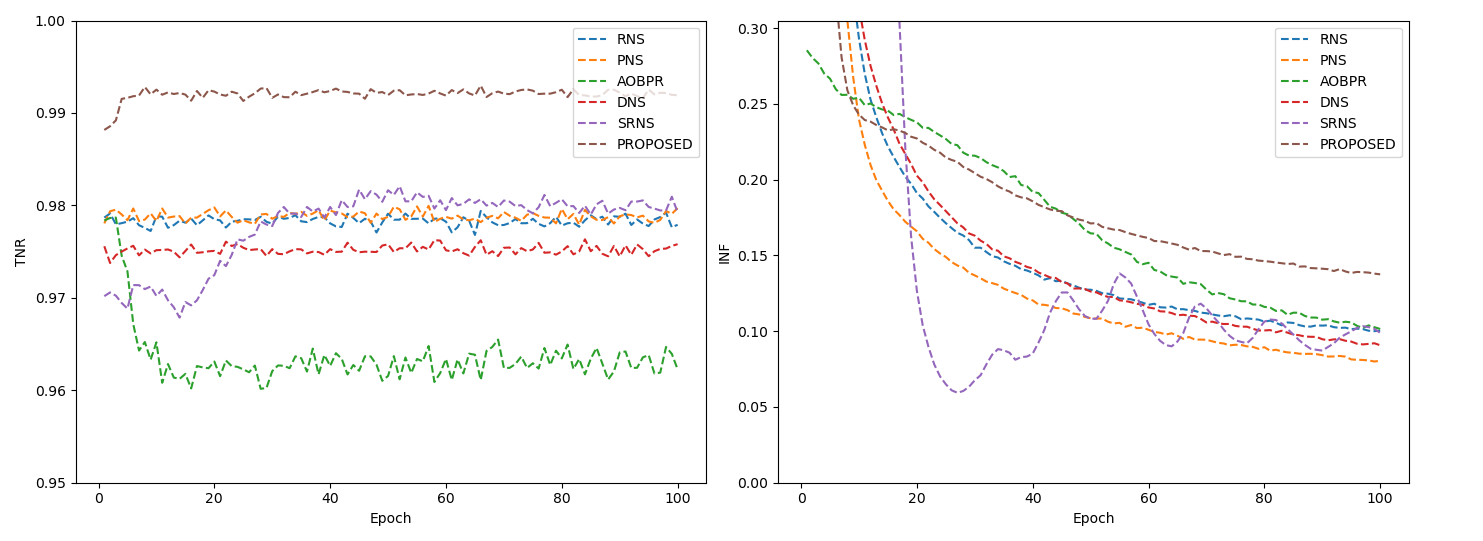
\includegraphics[width=\textwidth, height=0.35\textwidth]{3-tnr.png}
	\caption{不同方法的采样质量比较}
	\label{Fig:NegQua}
\end{figure*}
\subsubsection{负采样质量}
在本小结中,测试了两个采样准则:(i) 由公式\eqref{Eq:unbias}给出的\textit{后验概率准则}。(ii) 由公式\eqref{Eq:NegativeSam}给出的\textit{贝叶斯采样准则}。前者旨在选择真负样本,而后者旨在采样高质量的负样本实例。我们首先检查\textit{后验概率准则}是否能够选择真负样本实例,然后检查\textit{贝叶斯采样准则}是否能够选择高质量的负样本。

\textit{后验概率准则}通过从候选集$\mathcal{M}_u$中选择具有最大$\mathtt{unbias}(\cdot)$值的负样本实例来实现:
\begin{eqnarray} \label{Eq:PosteriorSam}
	j   &=&   \mathop{\arg\max}\limits_{l \in \mathcal{M}_u} \mathtt{unbias}(l)
\end{eqnarray}
$\mathcal{I}_u^-$是一个从$\mathcal{I}_u^-$中随机选择的负样本的小候选集,规模大小固定为5。\textit{贝叶斯采样准则}通过从候选集$\mathcal{M}_u$中选择具有最小条件采样风险$R(\cdot|i)$的负样本实例来实现:
\begin{eqnarray} \label{Eq:NegativeSam1}
	j  = \mathop{\arg\min}\limits_{l \in\mathcal{M}_u}~ \mathtt{info}(l)\cdot [1-(1+\lambda)\mathtt{unbias}(l)]
\end{eqnarray}
不同采样方法的采样质量展示在图~\ref{Fig:NegQua}中。

(i) 采样偏差:\textit{固定分布采样}(\textsf{RNS}和\textsf{PNS})表现相对中等。它们的真负样本率(TNR)在随机样本为真负样本的概率附近波动。\textit{困难负采样}(\textsf{AOBPR}和\textsf{DNS})表现最差。它们采用贪婪策略强调排名较高的负样本,也带来了更高的采样误差风险,正如我们在第~\ref{Sec:Dis}节中讨论的那样。\textsf{SRNS}利用预测分数方差的简单先验统计信息,限制了负样本分类的潜力,因为这种先验方差可能导致采样分布过于集中。提出的\textit{贝叶斯负采样}(\textsf{BNS})由于我们的贝叶斯负分类,TNR接近1,实现了最佳性能。

(ii) 采样质量:样本的信息量随训练时期的增加而降低。这是因为经过训练的推荐模型可能会将用户潜在感兴趣的伪负真负样本(参见图~\ref{Fig:DistributionStatistics})。在足够的训练时期后,\textsf{BNS}实现了最佳性能。\textit{困难负采样}(\textsf{AOBPR}和\textsf{DNS})受到最高采样偏差的惩罚更多。\textsf{SRNS}采用线性加权平均来结合信息性和方差,这可能不能保证采样无偏和信息丰富的实例

\subsubsection{超参数分析}\label{Appendix:Selection}
首先将候选集$\mathcal{M}_u$的大小固定为5,以研究$\lambda$对性能的影响。较大的$\lambda$值意味着更加强调来自真负样本的排名增益,而较小的$\lambda$值则更加关注避免采样假负样本的风险。从图~\ref{Fig:highperparameter}中可以观察到,当$\lambda$的值从0.1增加到1时,$NDCG@20$显著提高,并且在$\lambda=5$时达到最大值。

然后,将最优$\lambda$值固定为5,研究$\mathcal{M}_u$的大小对性能的影响,并在范围$\{1, 3, 5, 10, 15\}$内搜索$|\mathcal{M}_u|$的取值。需要注意的是,当$|\mathcal{M}_u|=1$时,提出的\textsf{BNS}变为经典的随机负采样(\textsf{RNS})。当$|\mathcal{M}_u|>1$时,贝叶斯采样准则开始发挥其样本筛选的作用。当$|\mathcal{M}_u|=|\mathcal{I}_u^-|$时,公式~\eqref{Eq:NegativeSam}中的采样器$h$是由公式~\eqref{Eq:OptimalSam}给出的最优采样器$h^*$。从图~\ref{Fig:highperparameter}中可以观察到,当$|\mathcal{M}_u|=5$或$10$时,$NDCG@20$达到最大值。为了降低时间复杂度,我们将$|\mathcal{M}_u|=5$。

\begin{figure*}[!]
	\centering
	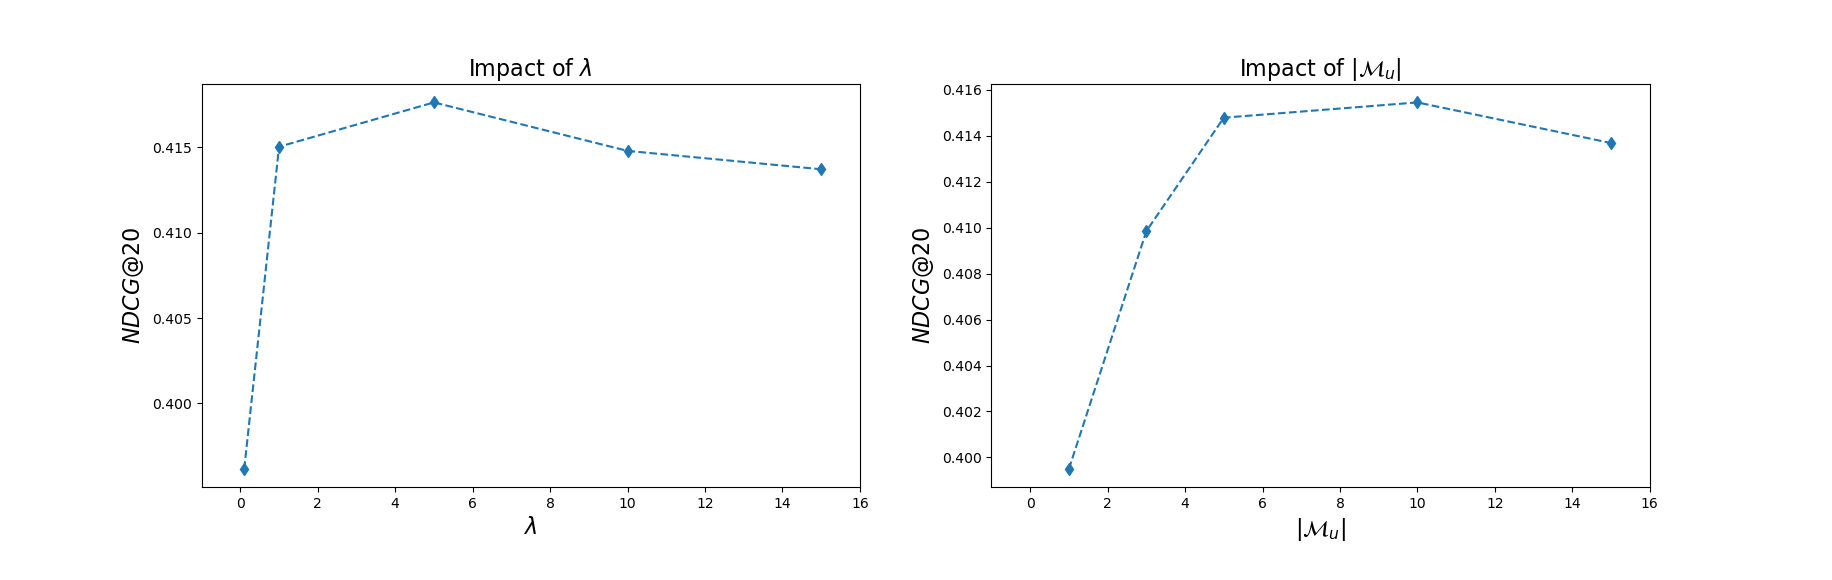
\includegraphics[width=\textwidth, height=0.3\textwidth]{3-highperparameter.png}
	\caption{参数$\lambda$和$|\mathcal{M}_u|$的影响}
	\label{Fig:highperparameter}
\end{figure*}
当$|\mathcal{M}_u| > 10$时,$NDCG@20$的值下降。这个实验结果与预期不符,因为$|\mathcal{M}_u|$值越大,越容易选择最优负样本。我们认为这是由于不可靠的先验概率$P_{fn}(l)$估计引起的。不可靠的先验信息进一步导致了由$F(\hat{x}_l)$表示的分类结果的偏差,进而导致了负信号$\mathtt{unbias}(\cdot)$的进一步偏离。过大的$|\mathcal{M}_u|$放大了负信号偏差的不利影响,导致性能下降。更多讨论可以在第~\ref{Appendix:Asymptotic}节中找到。

本节进一步研究了\textsf{BNS}对$\lambda$、样本信息$\hat{x}_l$和先验信息$P_{fn}(l)$的敏感性。
\begin{itemize}
	\item[-]\textsf{BNS}-1:$\lambda$的热启动。设置$\lambda = \max(10-\alpha \times \text{epoch}, 2)$,随着epoch数的增加,线性降低$\lambda$的值。即,在初始阶段,较大的$\lambda$强调对真负样本进行排名增益,而在后期阶段,较小的$\lambda$强调对假负样本进行采样损失。其中,$\alpha$选为0.1。
	\item[-]\textsf{BNS}-2:样本信息$\hat{x}_l$的热启动。我们首先采用\textsf{RNS}训练一个推荐模型一些epoch,以学习更可靠的样本信息$F(\hat{x}l)$,然后通过将其替换为我们的\textsf{BNS}来恢复训练。
	\item[-]\textsf{BNS}-3:无信息先验分布。对于这种情况,\textsf{BNS}简化为仅使用样本信息$\hat{x}l$进行负采样的\textsf{DNS}。对于单次随机试验,任何物品$l$被交互的概率为1/1682,即我们对任何负样本$l$无差别地设置$P_{fn}(l) = 1/1682$,其中1682是物品的总数。
	\item[-]\textsf{BNS}-4:职业信息增强的先验分布。在公式~\eqref{Eq:Prior}的基础上,我们添加了一个调整因子来改善$P_{fn}(l)$的估计:
	\[P{fn}(l) = \frac{pop_l}{N} \cdot (1 + \triangle o_{ul}),\]
	其中$\triangle o_{ul} = \frac{o_{ul} - \bar{o}l}{\max{o}{l}}$表示$u$的职业中对$l$的偏好次数与平均值之间的偏差。$o_{ul}$是具有与$u$相同职业的群体在物品$l$上的交互次数,$\bar{o}_l$是物品$l$被每个职业交互的平均次数。
\end{itemize}
实验结果见表~\ref{Exp:study}。以下是我们的发现:

\begin{table*}[h]
	\centering
	\caption{BNS负采样算法的消融实验}\label{Exp:study}
	\resizebox{1\textwidth}{!}{
		\begin{tabular}{lclccccccccccc}
			\toprule[1.2pt]
			\multirow{2}*{\textbf{Dataset}} & \multirow{2}*{\textbf{CF Model}} & \multirow{2}*{\textbf{ Method}} & \multicolumn{3}{c}{Top-5} &~& \multicolumn{3}{c}{Top-10}&~&\multicolumn{3}{c}{Top-20}\\ \cline{4-6} \cline{8-10} \cline{12-14}
			
			~ & ~ & ~ & Precision& Recall& NDCG& ~ &Precision& Recall& NDCG& ~ &Precision& Recall& NDCG \\ \hline
			
			\multirow{6}*{\textbf{100K}} & \multirow{6}*{\textbf{MF}} & RNS & 0.3900   &0.1301	&0.4143	&~&0.3363	&0.2164	&0.3967& ~&0.2724&0.3298&0.3962 \\
			~ & ~ & BNS    &0.4205	&0.1467	&0.4558&~	&0.3463	&0.2290	&0.4217& ~&0.2762&0.3466& 0.4176\\
			~ & ~ & BNS-1  &0.4237	&0.1471	&0.4551	&~&0.3495	&0.2305	&0.4238& ~&0.2762&0.3495&0.4197\\
			~ & ~ & BNS-2  &0.4148	&0.1456	&0.4449&~	&0.3411	&0.2245 &0.4132& ~&0.2738&0.3434&0.4125\\
			~ & ~ & BNS-3  &0.4048	&0.1392	&0.4266&~	&0.3423	&0.2282 &0.4043& ~&0.2720&0.3406&0.4030\\
			~ & ~ & BNS-4  &0.4262	&0.1478	&0.4566&~	&0.3486	&0.2305 &0.4235& ~&0.2792&0.3520&0.4216\\
			\cline{1-14}
			
			\bottomrule[1.2pt]
			
		\end{tabular}
	}
\end{table*}

%########################
\textbf{\textsf{BNS}对$\lambda$的敏感性}:$\lambda$的热启动取得了更好的性能(\textsf{BNS}-1)。较大的$\lambda$值意味着在采样风险和增益之间的权衡程度更高,即更加强调来自真负样本的排名增益而非假负样本的风险。结果显示,对于模型学习来说,困难样本是重要的,这与现有研究的发现一致~\cite{Ding:2020:NIPS,Park:2019:WWW}。建议采用$\lambda$的热启动策略:在初始阶段使用较大的值强化对困难样本的采样,而在后期阶段使用较小的$\lambda$以避免采样伪负例。

\textbf{\textsf{BNS}对先验概率$P_{fn}(\cdot)$的敏感性}:结果显示,在没有先验信息的情况下,\textsf{BNS-3}相对于标准的\textsf{BNS}性能较差,而在增强职业信息先验概率的情况下,\textsf{BNS-4}相对于标准的\textsf{BNS}性能更好。结果表明,\textsf{BNS}对先验概率敏感。先验信息影响负采样的机制是:不可靠的先验概率$P_{fn}(\cdot)$导致由$F(\hat{x}_\cdot)$表示的分类结果偏差,进而导致负信号$\mathtt{unbias}(\cdot)$的进一步偏离。过大的候选集$\mathcal{M}u$放大了负信号偏差的不利影响,导致性能下降。因此,如果先验概率$P{fn}(\cdot)$可靠,则选择更大的$\mathcal{M}_u$更好;否则,应选择适度大小的$\mathcal{M}u$。特别地,在非信息先验分布的情况下,\textsf{BNS}等效于\textsf{DNS}:\textsf{BNS}采样具有适当$F(\hat{x})$值的实例,而\textsf{DNS}采样具有适当排名位置的实例,而$F(\hat{x})$和排名位置具有一对一的映射关系。通过选择适当的$|\mathcal{M}u|$和$\lambda$,\textsf{BNS-3}的性能与\textsf{DNS}相当。我们建议选择最可靠的先验信息来建模$P{tn}(\cdot)$或$P{fn}(\cdot)$。

\textbf{\textsf{BNS}对样本信息$\hat{x}_l$的敏感性}:样本信息$\hat{x}$的热启动(\textsf{BNS-2})并没有像预期的那样取得更好的性能,我们认为有三个原因:(i) 初始训练阶段的随机采样难以采样到难负例,导致\textsf{BNS-2}的性能下降;(ii) $\hat{x}$是由先验概率和采样器$h$内生确定的,因此$\hat{x}$的热启动对最终的排名性能影响有限;(iii) 我们使用样本信息$F(\hat{x}\cdot)$的方式对$\hat{x}_\cdot$的微小变化不敏感,因此改进的$\hat{x}$对提高采样质量的影响有限。我们认为\textsf{BNS}具有对不同排名模型的鲁棒性,这是它对不同排名模型具有鲁棒性的重要体现,因为在不满足顺序关系的条件下(例如早期训练阶段或弱排名模型),\textsf{BNS}仍然能够利用先验信息采样高质量的负实例。

\subsubsection{向其他损失函数推广}\label{Appendix:LossFunc}
本小结检验\textsf{BNS}在其他损失函数中的适用性。我们选择了两个基于对比的损失函数,即二元交叉熵(BCE)损失和InfoNCE损失函数。我们使用矩阵分解模型作为编码器,并分别将BPR损失~\cite{Steffen:2009:UAI}替换为BCE损失~\cite{Zizhuo:2021:ICDM}和Info-NCE~\cite{Oord:2018:arxiv}损失。超参数保持与使用BPR损失时相同。具体而言,InfoNCE损失的负实例数量$N$固定为2。表~\ref{Exp:supp}展示了使用不同损失函数的结果。可以看出,与随机负采样\textsf{RNS}相比,\textsf{BNS}在所有三个损失函数中都取得了显著的改进,展示了\textsf{BNS}的良好适用性。
\begin{table*}[h]
	\centering
	\caption{不同损失函数下BNS负采样算法的表现}\label{Exp:supp}
	\resizebox{1\textwidth}{!}{
		\begin{tabular}{lclcccccccccccc}
			\toprule[1.2pt]
			
			\multirow{2}*{\textbf{Dataset}} & \multirow{2}*{\textbf{CF Model}} & \multirow{2}*{\textbf{Loss Function}} \multirow{2}*{\textbf{Method}} & \multicolumn{3}{c}{Top-5} &~& \multicolumn{3}{c}{Top-10}&~&\multicolumn{3}{c}{Top-20}\\ \cline{5-7} \cline{9-11} \cline{13-15}
			
			~ & ~ & ~ &~& Precision& Recall& NDCG& ~ &Precision& Recall& NDCG& ~ &Precision& Recall& NDCG \\ \hline
			
			\multirow{6}*{\textbf{100K}} & \multirow{6}*{\textbf{MF}} & \multirow{2}*{\textbf{BPR}} &RNS & 0.3900   &0.1301	&0.4143	&~&0.3363	&0.2164	&0.3967& ~&0.2724&0.3298&0.3962 \\
			
			~ & ~ & ~&BNS    &0.4205	&0.1467	&0.4558&~	&0.3463	&0.2290	&0.4217& ~&0.2762&0.3466& 0.4176\\\cline{3-15}
			
			~ & ~ & \multirow{2}*{\textbf{BCE}}&RNS    &0.3917	&0.1329	&0.4107&~	&0.3339	&0.2187	&0.3923& ~&0.2696&0.3315&0.3928\\
			~ & ~ & ~&BNS    &0.4226	&0.1454	& 0.4490&~	&0.3514&0.2299	&0.4205& ~&0.2821&0.3482& 0.4182\\\cline{3-15}
			~ & ~ & \multirow{2}*{\textbf{Info NCE}}&RNS    &0.3923	&0.1322	&0.4193&~	&0.3353	&0.2162	&0.3988& ~&0.2728&0.3376& 0.4012\\
			~ & ~ & ~&BNS    &0.4241	& 0.1471	&0.4523&~	&0.3519	&0.2281	&0.4226& ~&0.2817&0.3467& 0.4195\\
			\cline{1-15}
			
			\bottomrule[1.2pt]
			
		\end{tabular}
	}
\end{table*}

\subsubsection{渐近最优采样器}\label{Appendix:Asymptotic}
本小结展示所提出的采样器$h$通过理想先验概率$P_{fn}(l)$以渐进最优采样器$h^*$的过程。设置$P_{fn}(l) = (label(l)-0.2)^2$,即如果$l\in fn$,则$P_{fn}(l)=0.64$,否则$P_{fn}(l)=0.04$。通过逐渐增加$\mathcal{M}_u$的大小,以渐近最优采样器,其中$\lambda$固定为5。模拟结果如表~\ref{Table:asymptoticprocess}所示。通过增加候选集的大小,可以实现最优采样器$h^*$而不会降低排名性能。该结果验证了我们在第~\ref{Appendix:Selection}节中的分析。在具备一定程度的先验信息的情况下,即使对于简单的基于点乘的表示学习方法,\textsf{BNS}也能取得可观的性能,展示了负采样研究的巨大潜力。最优采样器(即$|\mathcal{M}_u| = |\mathcal{I}_u^-|$)的性能是基于点乘模型的经验上界。由于存在低秩约束和矩阵分解的有限表达能力,推荐性能无法达到1。
\begin{table*}[h]
	\centering
	\caption{向最优采样器的渐进过程}\label{Table:asymptoticprocess}
	\resizebox{1\textwidth}{!}{
		\begin{tabular}{lclccccccccccc}
			\toprule[1.2pt]
			\multirow{2}*{\textbf{Dataset}} & \multirow{2}*{\textbf{CF Model}} & \multirow{2}*{\textbf{\textsf{BNS} Size}} & \multicolumn{3}{c}{Top-5} &~& \multicolumn{3}{c}{Top-10}&~&\multicolumn{3}{c}{Top-20}\\ \cline{4-6} \cline{8-10} \cline{12-14}
			
			~ & ~ & ~ & Precision& Recall& NDCG& ~ &Precision& Recall& NDCG& ~ &Precision& Recall& NDCG \\ \hline
			
			\multirow{9}*{\textbf{100K}} & \multirow{9}*{\textbf{MF}} & $|\mathcal{M}_u| = 1$ & 0.3900   &0.1301	&0.4143	&~&0.3363	&0.2164	&0.3967& ~&0.2724&0.3298&0.3962 \\
			~ & ~ & $|\mathcal{M}_u| = 3$  &0.4909	&0.1567&0.5211&~	&0.4220	&0.2565	&0.4942& ~&0.3366&0.3872&0.4856\\
			~ & ~ & $|\mathcal{M}_u| = 5$ &0.5109	&0.1612	&0.5422	&~&0.4329	&0.2602	&0.5092& ~&0.3456&0.3925&0.4992\\
			~ & ~ & $|\mathcal{M}_u| = 10$  &0.5351	&0.1696	&0.5685&~	&0.4589	&0.2722 &0.5365& ~&0.3663&0.4081&0.5245\\
			~ & ~ & $|\mathcal{M}_u| = 20$  &0.5760	&0.1828	&0.6070&~	&0.4885	&0.2875 &0.5695& ~&0.3830&0.4196&0.5498\\
			~ & ~ & $|\mathcal{M}_u| = 50$  &0.6239	&0.1989	&0.6599&~	&0.5252	&0.3049 &0.6146& ~&0.4031&0.4312&0.5843\\
			~ & ~ & $|\mathcal{M}_u| = 100$   &0.6509	&0.2104	&0.6898&~	&0.5382	&0.3125 &0.6346& ~&0.4053&0.4321&0.5971\\
			~ & ~ & $|\mathcal{M}_u|= 500$  &0.6661	&0.2183	&0.7128&~	&0.5412	&0.3131 &0.6487& ~&0.4041&0.4300& 0.6076\\
			~ & ~ & $|\mathcal{M}_u|= |\mathcal{I}_u^-|$  &0.6674	&0.2184	&0.7133&~	&0.5429	&0.3140 &0.6495& ~&0.4041& 0.4292&0.6073\\
			\cline{1-14}
			
			\bottomrule[1.2pt]
			
		\end{tabular}
	}
\end{table*}

这些基准结果包括两个有启发性的消融实验的结果:(i) 只使用先验信息(物品流行度)的\textsf{PNS},以及 (ii) 只使用样本信息 $\hat{x}l$ 的\textsf{DNS}、\textsf{AOBPR}和\textsf{SRNS}。特别地,在无信息的先验分布的情况下,\textsf{BNS}退化为\textsf{DNS}。\textsf{BNS}根据适当的 $F(\hat{x})$-值对实例进行采样,而\textsf{DNS}根据适当的排名位置对实例进行采样,由于 $F(\hat{x})$ 和排名位置具有一对一的映射关系,因此它们实现了可比较的性能。上述两种范式的缺点是显而易见的:前者可以融合领域知识,但独立于模型状态,导致了静态的采样分布;后者利用了样本信息,但忽略了先验知识,在富有辅助信息的场景中,这将导致性能下降。所提出的\textsf{BNS}从贝叶斯的角度结合了先验信息和样本信息,并以赋予负信号$\mathtt{unbias}(l)$以后验概率的内涵。本章认为\textsf{BNS}的性能改进源于三个方面:(i) 先验信息 $P{tn}(l)$ 或 $P_{fn}(l)$,以及 (ii) 使用样本信息 $\hat{x}_l$。(iii) \textsf{BNS}是最小化经验采样风险的理论最优采样器。

\section{本章小结}\label{Sec:Conclusion}
本章定义了一个与模型无关的后验概率估计,作为定量的负信号度量。而后提出了贝叶斯负采样规则,这是最小化经验采样风险的理论最优的采样规则。\textsf{BNS}的贡献在于以后验概率的意义上指定了负信号度量。从贝叶斯的角度,\textsf{BNS}通过结合静态的先验信息和动态的样本信息,统一了现有的两种提取负信号的范式。需要注意的是,\textsf{BNS}并未具体指定建模先验概率的方法。相反,$P_{tn}(l)$(或$P_{fn}(l)$)为使用辅助信息建模先验概率的方法提供了接口。此外,只要模型旨在将正例的得分高于负例,\textsf{BNS}也可以应用于其他基于对比的损失函数。

需要指出的是,负采样算法与基于GPU批量并行计算Mini-Batch模型并不兼容。典型的动态负采样需要先计算当前轮次样本得分(正向传播),然后采样负例。而基于Mini-Batch模型需要把样本固定到DataLoader中,才能进行正向传播预测得分,这与动态负采样机制有所冲突。而动态负采样需要先得到预测得分,然后再采样负例。通常是把很多的候选负样本装载入Dataloader,并计算额外样本的预测得分来实现动态负采样,造成了额外的计算和存储开销。此外,本章所假设的真负例和伪负例的相似度分数的序关系是一个理想的情况,是一个比较强的假设。后面的章节将解决这两个局限性。

\chapter{成对损失函数校正研究}
\label{cha:fourthsection}
从成对比较中学习对比表示(contrastive representations)在自然语言处理、计算机视觉和信息检索等多个领域取得了显著的成功。基于成对学习的协同过滤算法也根植于这一范式。一个重要的问题是数据集普遍是positive-unlabeled,即负例未标注,这经常导致随机选择的负例包含了伪负例,并且不可避免地引入导致学到有偏的嵌入,从而影响下游的分类、排序任务的泛化性能。上一章介绍了最优负采样准则,但是负采样算法不适用于基于GPU批量并行计算的mini-batch模型,往往以额外的存储开销和计算开销为代价实现。本章采用了一个截然不的技术路径纠正采样偏差,得到了一种校正后的成对学习损失函数,称为去偏成对损失(Debiased Pairwise Loss, DPL)。DPL的核心思想是纠正由于伪负例引起的偏倚概率估计,从而修正梯度,使其逼近完全监督数据的梯度。对五个公共数据集进行的实验研究验证了所提出的学习方法的有效性。

\section{引言}
成对学习鼓励编码器对样本之间的差异特征进行编码,而不是对个体样本的像素级特征进行编码,通常能够获得更好的泛化性能,尤其是在样本的绝对值较少有意义的场景下~\cite{Wang:2020:ICML,McFadden:1974:FE,gutmann:2012:JMLR,Liu:2021:TKDE,Wang:2020:ICML}。成对学习已成为许多现代机器学习算法的基本组成部分,并在自然语言处理、图像和语音识别以及推荐系统等诸多领域取得了重大进展~\cite{Oord:2018:arxiv,Wang:2020:ICML,He:2020:CVPR,Steffen:2009:UAI}。在协同过滤中,成对学习被广泛应用于预测排序,其中最著名的方法是贝叶斯个性化排名(BPR)~\cite{Steffen:2009:UAI}。从统计角度来看,BPR最大化了观察到的正负样本的后验概率。从数值计算角度来看,BPR损失函数鼓励模型正例的得分高于负例。在嵌入空间中,BPR损失的目标是将正例的嵌入拉近到锚点(即用户),同时将负例的嵌入推离锚点。

然而,用户通常只通过交互行为(如点击、购买或评分)来表达他们的偏好或兴趣,从而仅提供正反馈。因此,训练集通常以正无标签(PU)数据的形式存在。针对这一在机器学习的诸多领域普遍存在的问题,负采样技术被广泛研究。负采样可以分为两种类型:第一种是静态负采样,它使用固定的采样分布,利用与模型的训练状态无关的某种辅助信息,可能导致简单的样本,相比之下,与动态负采样相比,静态负采样的性能往往较差。此外,静态负采样严重依赖于辅助信息作为有效的监督信号,而这些监督信息在大多数场景下是难以获取的。动态负采样使用与模型相关的信息(如预测得分)动态调整采样分布,旨在采样具有高得分或排名靠前的困难负样本,以提高性能,但容易遇到伪负例~\cite{Ding:2020:NIPS}。此外,基于GPU批量计算的mini-batch训练与动态负采样不兼容。矛盾的关键在于,mini-batch训练要求训练之前将样本固定加载到数据加载器中,然后进行正向预测得分和反向传播更新参数;而动态负采样要求先正向预测得分,然后采样样本。动态负采样通常需要额外的计算和存储开销,例如存储先前训练轮次的预测得分~\cite{Ding:2020:NIPS},或计算mini-batch之外样本的预测得分。

本章聚焦于没有任何辅助信息用于监督的最一般形式的隐式反馈数据,提出了一种从无标签数据中纠正采样偏差的方法,从而为成对学习提供了一种修改后的损失函数,称为去偏成对损失(Debiased Pairwise Loss,DPL)。DPL的核心思想是修正由于假负例导致的概率估计偏差,从而修正梯度以近似完全监督数据的梯度。DPL不需要额外的辅助信息进行监督,也不需要过多的存储和计算开销。

\section{成对损失优化目标分析}
将用户物品对$(u,i)$表示为样本$\mathbf{x}$,其中$u\in \mathcal{U}$,$i\in \mathcal{I}$。令$\mathcal{X}= \{\mathbf x|u\in \mathcal{U}, i\in \mathcal{I}\}$表示包含所有用户物品对的样本空间,$\mathcal{Y} =\{-1,+1\}$表示类别标签,指示用户是否喜欢该物品。决策函数$g:\mathcal{X} \rightarrow \mathbb{R}$是一个实值函数,为每个交互分配一个预测的偏好水平$g(\mathbf x) \in \mathbb{R}$。将正例的类条件密度表示为$p^+(\mathbf x) = p(\mathbf x|+1)$,将负例的类条件密度表示为$p^-(\mathbf x) = p(\mathbf x|-1)$。因此,边际分布$p(\mathbf x)=p^+(\mathbf x) \tau^+ +p^-(\mathbf x)\tau^-$,其中$\tau^+ = 1-\tau^-$是先验概率$p(c(\mathbf{x}) = +1)$。

在隐式协同过滤中,通过对两个随机样本$(\mathbf{x}^+, \mathbf{x}^-)$进行成对比较,通过预测的偏好水平$g(\mathbf x) \in \mathbb{R}$以预测个性化排序。BPR\cite{Steffen:2009:UAI}采用了著名的Bradley-Terry模型建模观察到正例$\mathbf{x}^+$优于负例$\mathbf{x}^-$的似然
\begin{eqnarray}\label{eq:bpr}
	\mathcal{L}_{BPR} &=& - \mathbb{E}_{\substack{\mathbf x^+ \sim p^+(\mathbf x) \\ \mathbf x^- \sim p^-(\mathbf x^-)}} \log \sigma(g(\mathbf{x}^+) - g(\mathbf{x}^-)) \\
	&=&  - \mathbb{E}_{\substack{\mathbf x^+ \sim p^+(\mathbf x) \\ \mathbf x^- \sim p^-(\mathbf x)}}\log \frac{1}{1+\exp(-g(\mathbf{x}^+) + g(\mathbf{x}^-))} \nonumber \\
	&=&  - \mathbb{E}_{\substack{\mathbf x^+ \sim p^+(\mathbf x) \\ \mathbf x^- \sim p^-(\mathbf x^-)}}\log\frac{\exp(g(\mathbf{x}^+))}{\exp(g(\mathbf{x}^+))+\exp( g(\mathbf{x}^-))} \label{eq:infonce1}
\end{eqnarray}

值得注意的是,式\eqref{eq:infonce1}是贝叶斯个性化排名(BPR)损失的等价形式,它与噪声对比估计(NCE)损失\cite{Gutmann:2010:ICAIS}完全相同,而NCE损失是InfoNCE损失\cite{Oord:2018:arxiv}在只有一个负例(即N=1)的特殊情况。此外,在协同过滤的场景中,用户和物品构成一个二部图,通常只选择用户嵌入作为锚点。在理想情况下,正例是从已有交互的物品中进行采样的,表示为$\mathbf{x}^+ \in \mathcal{D}^+$,而负例是从用户不喜欢的物品中进行采样的,表示为$\mathbf{x}^- \in \mathcal{D}^-$。因此,式\eqref{eq:bpr}的对应的经验估计可以表示为:
\begin{eqnarray}\label{eq:bpr_emp}
	\mathcal{L}_\text{BPR} =- \frac{1}{|\mathcal{D}^+|\times |\mathcal{D}^-|} \sum_{\mathbf{x}^+ \in \mathcal{D}^+}\sum_{\mathbf{x}^- \in \mathcal{D}^-} && \ln \sigma(g(\mathbf{x}^+) - g(\mathbf{x}^-)) \nonumber  - \lambda ||\Theta||^2,
\end{eqnarray}
其中,$\lambda ||\Theta||^2$ 是正则化项,用于平衡方差和偏差,避免过拟合。特别地,正则化项$\lambda ||\Theta||^2$等价于高斯分布的先验密度的对数,从而为式\eqref{eq:bpr_emp}提供了基于后验概率的解释。在原始的贝叶斯个性化排名(BPR)论文\cite{Steffen:2009:UAI}中,式\eqref{eq:bpr_emp}被解释为观测到的有序对的最大后验估计。

在实际中,由于缺乏标记的负例样本,在优化式\eqref{eq:bpr_emp}时,只能从未标记的数据中采样负例样本,导致以下偏倚的优化目标:
\begin{eqnarray}\label{eq:bpr_emp_biased}
	\mathcal{L} =- \frac{1}{|\mathcal{D}^+|\times |\mathcal{D}^u|} \sum_{\mathbf{x}^+ \in \mathcal{D}^+}\sum_{\mathbf{x} \in \mathcal{D}^u} && \ln \sigma(g(\mathbf{x}^+) - g(\mathbf{x})) - \lambda ||\Theta||^2,
\end{eqnarray}

接下来,考察偏倚的优化目标对学习到的用户-物品嵌入$\Theta$的影响:
\begin{eqnarray}
	\frac{\partial \mathcal{L}}{\partial \Theta} &=& \frac{\partial \mathcal{L}_\text{BPR}}{g(\mathbf{x})}\cdot\frac{g(\mathbf{x})}{\Theta}  \\
	&=& [1-\sigma(g(\mathbf{x}^+) - g(\mathbf{x})) ]\cdot\frac{g(\mathbf{x})}{\Theta}  \label{eq:graident}
\end{eqnarray}
式\eqref{eq:graident}是微分链式法则的结果,其中第一项$[1-\sigma(g(\mathbf{x}^+) - g(\mathbf{x}))]$由损失函数的形式决定,第二项$\frac{g(\mathbf{x})}{\Theta}$由决策函数决定。对于固定的模型,第二项保持不变。

在式\eqref{eq:graident}的第一项中,实值sigmoid函数$\sigma(g(\mathbf{x}^+) - g(\mathbf{x})) \in [0,1]$被解释为用户偏好正例强于负例的似然\cite{Steffen:2009:UAI},是优化目标。然而,由于$\mathbf{x}$是未标记样本,它以$\tau^+$的先验概率是正样本,这导致了概率的偏倚估计。

图\ref{fig:event}提供了一个阐释性的例子说明为何使用正例-未标记数据对计算的值$\sigma(g(\mathbf{x}^+) - g(\mathbf{x}))$是一个偏倚的概率估计。“偏好正例强于负例的似然”,描述的是事件$\mathcal{A}_1(+,-)$的概率,这是优化目标。然而在实践中,给出的是正例-未标注样本对,导致成对学习优化的是事件$\mathcal{A}(+,u)$的概率。然而,事件$\mathcal{A}(+,u)$的概率和事件$\mathcal{A}_1(+,-)$的概率是不等价的,根据事件的可列可加性原理,事件$\mathcal{A}(+,u) = \mathcal{A}_1(+,-) + \mathcal{A}_2(+,+)$。这个偏差,导致了偏倚的“偏好正例强于负例”的概率估计,从而导致了有偏的最大似然/后验的优化目标。直观地说,偏倚的$\sigma(g(\mathbf{x}^+) - g(\mathbf{x}))$值会导致不正确的梯度大小${\partial \mathcal{L}_\text{BPR}}/{\partial \Theta}$,从而在执行随机梯度下降学习算法时导致不准确的用户-物品表示。
%%%%%%%%%%%%%%%%%%%%%%%%%%%%%%%%%%%%%%%%%%%%%%%%%%%%%%%%%%%
\begin{figure}[h!]
	\centering
	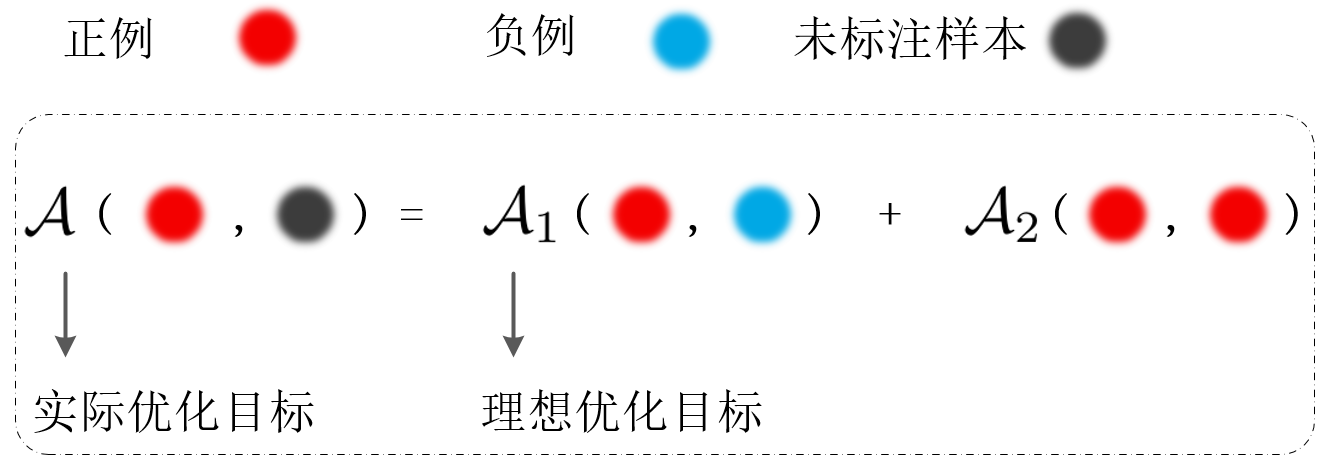
\includegraphics[width=0.8\textwidth]{4-event.png}
	\caption{偏倚的概率估计的示意图} 
	\label{fig:event}
\end{figure}
%%%%%%%%%%%%%%%%%%%%%%%%%%%%%%%%%%%%%%%%%%%%%%%%%%%%%%%%%%%

为了使数学表达中保持简洁,本章定义一个映射$h: \mathcal{X}\times\mathcal{X} \rightarrow \sigma(g(\mathbf{x}^+) - g(\mathbf{x}))$,将两个样本映射到一个sigmoid函数。问题变成如何使用来自正例和未标记样本群体的样本来近似估计$h(\mathbf{x}^+,\mathbf{x}^-)$的值。具体而言,给定一组正例样本$\{\mathbf{x}_i\}_{i=1}^M$和一组未标记样本$\{\mathbf{x}_j\}_{j=1}^N$,目标是估计$h(\mathbf{x}^+,\mathbf{x}^-)$的值,从而可以校正梯度以近似完全监督数据的梯度,从而提高学习到的用户-物品表示的泛化性能。

\section{去偏成对学习算法}
为了使用来自正例-未标记样本对来近似估计$h(\mathbf{x}^+,\mathbf{x}^-)$的值,首先建立正例-未标记样本对的联合分布$p_\textsc{pu}$与正例-负例样本对的联合分布$p_\textsc{pn}$之间的关系。

样本对的第一个样本,记为$\mathbf x_1$,是从正类条件概率$p^+(\mathbf x)$中确定性地抽取的,而第二个样本,记为$\mathbf{x}_2$,是从边缘分布$p(\mathbf{x})$中抽取的。因此,正例-未标记样本对的联合分布$p\textsc{pu}$可以表示如下:
\begin{eqnarray}
	p_\textsc{pu}(\mathbf{x}_1, \mathbf{x}_2) &=& p^+( \mathbf{x}_1) p( \mathbf{x}_2)  \label{eq:independent} \\
	&=& p^+( \mathbf{x}_1) [p^+(\mathbf x_2) \tau^+ +p^-(\mathbf x_2)\tau^- ] \label{eq:full}\\
	&=& \tau^+p^+( \mathbf{x}_1) p^+(\mathbf x_2) + \tau^-p^+( \mathbf{x}_1)p^-(\mathbf x_2) \label{eq:pnpp}
\end{eqnarray}
式\eqref{eq:independent}是由于$(\mathbf{x}_1, \mathbf{x}_2)$是独立抽取的。此外,式\eqref{eq:full}是边缘分布$p(\mathbf{x})$的完整概率分解。重新整理式\eqref{eq:pnpp},可以建立所需的正例-负例样本对的联合分布$p_\textsc{pn}(\mathbf{x}_1, \mathbf{x}_2)$与正例-未标记样本对的联合分布$p_\textsc{pu}(\mathbf{x}_1, \mathbf{x}_2)$之间的关系,表示为
\begin{eqnarray}\label{eq:jointpn}
	p_\textsc{pn}(\mathbf{x}_1, \mathbf{x}_2)  &=& p^+( \mathbf{x}_1)p^-(\mathbf x_2) \nonumber \\
	&=& \frac{1}{\tau^-}[p_{\textsc{pu}}(\mathbf{x}_1, \mathbf{x}_2)- \tau^+p^+( \mathbf{x}_1) p^+(\mathbf x_2)] \label{eq:pndist}
\end{eqnarray}

因此,$h(\mathbf x_1,\mathbf x_2)$相对正例-负例样本对的联合分布$p_\textsc{pn}(\mathbf{x}_1, \mathbf{x}_2)$上的期望,即理想的优化目标“用户喜欢正例$\mathbf{x}_1$优于负例$\mathbf{x}_2$”的概率期望值,可以计算如下:
\begin{eqnarray}
	&&\mathbb{E}_{ p_\textsc{pn}(\mathbf{x}_1, \mathbf{x}_2)} h(\mathbf{x}_1,\mathbf{x}_2)\\
	&=& \int_{\mathbf{x}_1}\int_{\mathbf{x}_2}   h(\mathbf{x}_1,\mathbf{x}_2) p_\textsc{pn}(\mathbf{x}_1, \mathbf{x}_2) d{\mathbf{x}_1}d{\mathbf{x}_2} \\
	&=&\int_{\mathbf{x}_1}\int_{\mathbf{x}_2}   h(\mathbf{x}_1,\mathbf{x}_2) [\frac{1}{\tau^-}p_{\textsc{pu}}(\mathbf{x}_1, \mathbf{x}_2)- \frac{\tau^+}{\tau^-}p^+( \mathbf{x}_1) p^+(\mathbf x_2)]d{\mathbf{x}_1}d{\mathbf{x}_2} \\
	&=&\int_{\mathbf{x}_1}\int_{\mathbf{x}_2}   h(\mathbf{x}_1,\mathbf{x}_2) [\frac{1}{\tau^-}p_{\textsc{pu}}(\mathbf{x}_1, \mathbf{x}_2) d{\mathbf{x}_1}d{\mathbf{x}_2}- \int_{\mathbf{x}_1}\int_{\mathbf{x}_2} \frac{\tau^+}{\tau^-}p^+( \mathbf{x}_1) p^+(\mathbf x_2)]d{\mathbf{x}_1}d{\mathbf{x}_2} \\
	&=& \frac{1}{\tau^-}\mathbb{E}_{ p_\textsc{pu}(\mathbf{x}_1, \mathbf{x}_2)} h(\mathbf{x}_1,\mathbf{x}_2) -\frac{\tau^+}{\tau^-} \mathbb{E}_{ p_\textsc{pp}(\mathbf{x}_1, \mathbf{x}_2)} h(\mathbf{x}_1,\mathbf{x}_2) \label{eq:expec}
\end{eqnarray}
式\eqref{eq:expec}的第一项表示正例-未标记样本对的期望,在给定第一个正例样本$\mathbf{x}^+$的情况下,可以使用$N$个未标记样本$\{\mathbf{x}_n\}_{n=1}^N$进行经验估计:
\begin{eqnarray}
	\mathbb{E}_{ p_\textsc{pu}(\mathbf{x}_1, \mathbf{x}_2)} h(\mathbf{x}_1,\mathbf{x}_2) &=& \frac{1}{N} \sum_{n=1}^{N} h(\mathbf{x}^+,\mathbf{x}_n)\label{eq:epu},
\end{eqnarray}
式\eqref{eq:expec}的第二项表示正例-正例样本对的期望,在给定第一个正例样本$\mathbf{x}^+$的情况下,可以使用额外的$M$个正例样本${\mathbf{x}'_n}_{m=1}^M$进行经验估计
\begin{eqnarray}
	\mathbb{E}_{ p_\textsc{pp}(\mathbf{x}_1, \mathbf{x}_2)} h(\mathbf{x}_1,\mathbf{x}_2)  &=& \frac{1}{M} \sum_{m=1}^{M} h(\mathbf{x}^+,\mathbf{x}_m^{\prime})\label{eq:epp}.
\end{eqnarray}

将式\eqref{eq:epu}和式\eqref{eq:epp}代入式\eqref{eq:expec},可以得到理想的优化目标“用户喜欢正例$\mathbf{x}_1$优于负例$\mathbf{x}_2$”的概率期望值的经验估计:
\begin{eqnarray}\label{eq:est}
	\hat{P}_\textsc{pn} = \frac{1}{N\tau^-}
	\sum_{\mathbf{x} \in \mathcal{D}^u}h(\mathbf{x}^+,\mathbf{x})  - \frac{\tau^+}{M\tau^-}\sum_{\mathbf{x}^\prime\in \mathcal{D}^+}h(\mathbf{x}^+, \mathbf{x}^\prime)
\end{eqnarray}

如上所示,方程中的第一项使用正例-未标记样本对进行计算,但额外添加了一个校正项,以抵消由于未标记集合中包含错误的负例样本而产生的偏倚似然估计。式\eqref{eq:est}中的第二项,从正例-正例对计算的校正项可能看起来奇怪,图\ref{fig:auc}对这个校正项提供了一个直观解释。

考虑一个正例-未标记的数据集,其中$\{x_1, x_2\}$是正例样本,$\{x_3, x_4, x_5\}$是未标记样本。在训练过程中,无法访问未标记样本$\{x_3, x_4, x_5\}$的真实标签。式\eqref{eq:est}的第一项描述的是使用正例样本和未标记数据对计算的AUC风险,即把不可微的0-1损失替换为可微的\textsf{sigmoid}损失所得到的AUC值,记为$AUC_\textsc{pu}$。根据AUC的定义,$AUC_\textsc{pu}$可以分解为两个项的和组成。第一个项是使用正例-负例(PN)数据对计算的干净AUC估计,表示为$AUC_\textsc{pn}$。第二个项是使用正例-正例(PP)数据对计算的伪AUC估计,表示为$AUC_\textsc{pp}$。为了优化干净AUC,应该从$AUC_\textsc{pu}$中减去$AUC_\textsc{pp}$。而减去的补偿项目,正是由式\eqref{eq:est}的第二项基于正例-正例对计算的伪AUC估计。

%%%%%%%%%%%%%%%%%%%%%%%%%%%%%%%%%%%%%%%%%%%%%%%%%%%%%%%%%%%
\begin{figure*}[h!]
	\centering
	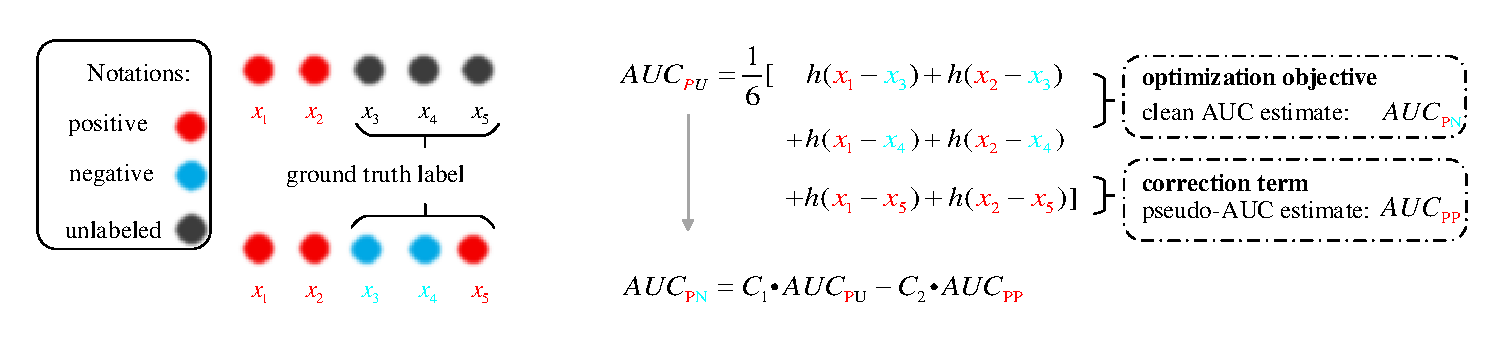
\includegraphics[width=\textwidth]{4-unbiasedAUC.pdf}
	\caption{去偏成对损失的示意图} 
	\label{fig:auc}
\end{figure*}
%%%%%%%%%%%%%%%%%%%%%%%%%%%%%%%%%%%%%%%%%%%%%%%%%%%%%%%%%%%
有了式\eqref{eq:est}给出的优化目标“用户喜欢正例$\mathbf{x}_1$强于负例$\mathbf{x}_2$”的估计,可以很容易进行极大似然估计。按照BPR的做法,本章也最大化对数似然,那么去偏的成对损失(Debiased Pairwise Loss,DPL)的最终经验形式如下所示:
\begin{eqnarray}\label{eq:dpl}
	\mathcal{L}_\textsc{dpl}=- \frac{1}{|\mathcal{D}^+|\times |\mathcal{D}^u|} \sum_{\mathbf{x}^+ \in \mathcal{D}^+}\sum_{\mathbf{x} \in \mathcal{D}^u} && \ln \hat{P}_\textsc{pn}.
\end{eqnarray}

\section{算法实现与时间复杂度分析}
在使用BPR损失进行训练时,对于每个$(u,i)$对,需要一个负样本$j$,从而形成一个$(u,i,j)$的训练三元组。为了解决采样偏差,DPL损失要求对于每个$(u,i)$对,额外采样$M\geq 1$个正例和$N\geq1$个负例。遵循与BPR相同的数据条目格式,每个DPL数据条目被组织为$(u,i,i_1,i_2,\cdots,i_M,j_1,j_2,\cdots,j_N)$。这可以通过重写\verb|Dataloader|的\verb|collate_fn|函数,实现将一个批量大小为bs个交互$(u,i)$的mini-batch数据,改写为含有bs个数据条目为$(u,i,i_1,i_2,\cdots,i_M,j_1,j_2,\cdots,j_N)$的mini-batch数据。算法伪码如下:
\begin{algorithm}[!]
	\caption{Pytorch的collate\_fn函数重写}\label{4Alg2:1}
	\KwIn{含有bs个交互$(u,i)$的mini-batch数据$\mathcal{R}$,批量大小bs,物品集合$\mathcal{I}$,用户正例集合$\mathcal{I}_u^+$。}
	\KwOut{含有bs个条目为$(u,i,i_1,i_2,\cdots,i_M,j_1,j_2,\cdots,j_N)$的mini-batch数据$\mathcal{R}\prime$。}
	\For{$(u,i) \in \mathcal{R}$}
	{
		~~从正例集合$\mathcal{I}_u^+$中随机采样M个正例$i_1,i_2,\cdots,i_M$;\\
		从未标注样本集合$\mathcal{I}_u^+$中随机采样N个未标注样本$j_1,j_2,\cdots,j_N$;\\
		将交互$(u,i)$、M个正例、N个负例拼接为1个数据条目;\\
		将该数据条目添加到$\mathcal{R}\prime$中;
	}
	\KwResult{含有bs个条目为$(u,i,i_1,i_2,\cdots,i_M,j_1,j_2,\cdots,j_N)$的mini-batch数据$\mathcal{R}\prime$。}
\end{algorithm}

因此,每个mini-batch数据结构组织如下:
\begin{eqnarray}\label{eq:mini}
	\text{batch size}\left\{ \left[\begin{array}{cccccccccc}
		u^{1} & {i}   &i_{1} & i_{2} & \ldots &i_{M} &   j_{1}& j_{2} & \ldots &j_{N} \\
		u^{2} & i & i_{1}& i_{2} & \ldots &i_{M} &  j_{1}& j_{2} & \ldots &j_{N} \\
		\vdots & \vdots & \vdots & \vdots &\ddots & \vdots & \vdots & \vdots & \ddots & \vdots \\
		u^{bs} & i & i_{1}& i_{2} & \ldots &i_{M} &  j_{1}& j_{2} & \ldots &j_{N} 
	\end{array}\right]\right.
\end{eqnarray}
每个数据条目包括N个未标记的样本$j_1,j_2,\cdots,j_N$,可以计算相应的N个预测得分 $\hat{x}{j}^1,\hat{x}{j}^2,\cdots,\hat{x}_{j}^N$。对于给定的正例样本 $(u,i)$,其得分为 $\hat{x}_i$,可以基于N个负例样本的预测得分得到N个PU概率值。因此,基于mini-batch估计的PU概率值为
\[\hat{P}_\textsc{pu} = \frac{1}{N} \sum_{n=1}^{N}\sigma (\hat{x}_i - \hat{x}_{j}^n)\]
类似地,可以计算出M个正例$i_1,i_2,\cdots,i_M$ 对应的M个预测得分 $\hat{x}{i}^1,\hat{x}{i}^2,\cdots,\hat{x}_{i}^M$,相应地,计算PP概率值估计为:
\[\hat{P}_\textsc{pp} = \frac{1}{M} \sum_{m=1}^{M}\sigma (\hat{x}_i - \hat{x}_{i}^m)\]

因此,经过校正后的理想的优化目标为:
\[\hat{P}_\textsc{pn} = \frac{1}{\tau^-}
\hat{P}_\textsc{pu} - \frac{\tau^+}{\tau^-}\hat{P}_\textsc{pp} \]
和BPR一样最大化对数似然,只需要对上式求对数后,执行梯度下降,基于Pytorch矩阵运算的算法伪码如下:
\begin{algorithm}[!]
	\small
	\caption{去偏成对学习算法(DPL)伪代码}\label{4-Alg:2}
	\KwIn{Mini-batch数据 $\mathcal{R}\prime$如式\eqref{eq:mini}所示, 评分函数$s(\cdot)$,额外正例数量M,额外负例数量N,正例类先验$\tau^+$,批量大小bs。}
	\KwOut{模型参数$\Theta \in \mathbb{R}^d$}
	\For{迭代次数$t= 1,2,...,T$}{
		~~从训练集中抽样一个mini-batch数据 $\mathcal{R}\prime$如式\eqref{eq:mini}所示;\\
		正向计算评分scores = s ($\mathcal{R}\prime$);   \# [bs * (1+M+N)] \\
		pos\_scores = scores[: , : M+2];   \# [bs * (1+M)]  \\
		neg\_scores = scores[: , M+2:]; \# [bs * N] \\
		pu\_prob = sigmoid(pos\_scores[:, 0:1] - neg\_scores); \# [bs*N] \\ 
		pp\_prob = sigmoid(pos\_scores[:, 0:1] - pos\_scores[:,1:]);  \# [bs*M]  \\
		pn\_prob = pu\_prob.mean(dim=-1)/(1-tau) - $\tau^+ \cdot$ pp\_prob.mean(dim=-1)/(1-tau); \#[bs, ] \\
		dpl\_loss = - log (pn\_prob).mean(); \\
		根据dpl\_loss相对于$\Theta$的梯度更新参数;
	}
	\KwResult{用户和物品表示$\Theta$。}
\end{algorithm}

\textbf{复杂度}:首先分析基线方法BPR的复杂度,该复杂度与评分函数$s$有关。这里,以维度$d$的矩阵分解作为示例,这个分析可以很容易地扩展到其他模型。给定一个批量大小为$bs$的$(u,i,j)$的训练三元组,前向评分计算涉及到总共$2\times bs$个得分预测,因此时间复杂度为$\mathcal O(2 bs\times d)$。在反向传播中,最多更新$3 \times bs$个嵌入,涉及总共$5bs\times d$次操作,因此BPR的时间复杂度为$\mathcal O(bs\times d)$。类似地,对于DPL,一个小批量数据涉及到总共$(M+N+1)\times bs$个评分计算和$(M+N+2)\times bs$个嵌入更新,涉及总共$(2M+2N+3)\times bs\times d$个操作,时间复杂度为$\mathcal O(bs\times d)$,因为在实践中通常将$M$和$N$设置为小的常数,例如$M=3$和$N=3$。特别地,当$M=0$且$N=1$时,DPL涉及的操作数量与BPR相同。因此,相对于BPR,DPL具有严格的线性复杂度,没有任何mini-batch数据之外的计算或者存储开销。而前面的负采样算法,由于涉及计算用户每个训练三元组中用户$u$对应的评分向量,而推荐中,物品数量通常非常大,导致了时间复杂度的增加。

\section{去偏成对损失的理论分析}
DPL的主要思想是改进使用正例-未标记数据对(PU)计算的偏倚概率$P_\textsc{pu}$。通过采样额外的正例和负例样本进行来估计式\eqref{eq:est}所给出的理想优化目标“用户喜欢正例$\mathbf{x}_1$优于负例$\mathbf{x}_2$”的概率$\hat P_\textsc{pn}$,然后用其替代原始的偏倚概率估计$P_\textsc{pu}$。为了证明$\hat P_\textsc{pn}$是一个良好的估计量,首先证明$\hat P_\textsc{pn}$是AUC风险的无偏估计。
\begin{lemma}\label{lemma:auc} 设正例$\mathbf{x}^+$是从正例的类条件概率分布$p^+(\mathbf{x})$独立采样的样本, 未标注样本$\mathbf{x}$是从边缘分布$p(\mathbf{x}) = \tau^+ p^+(\mathbf{x})+ \tau^- p^-(\mathbf{x})$独立采样的样本。 那么公式~\eqref{eq:est}给出的$\hat P_\textsc{pn}$是无偏的AUC风险估计:
	\[\mathbb{E}\hat P_\textsc{pn} = R_{AUC}\]
	\begin{proof}
		\begin{eqnarray}
			\mathbb{E}\hat P_\textsc{pn} &=& \int_{\mathbf{x}^+} [\frac{1}{N\tau^-}
			\sum_{\mathbf{x} \in \mathcal{D}^u} \mathbb{E}_{\mathbf{x}\sim p}h(\mathbf{x}^+,\mathbf{x}) - \frac{\tau^+}{M\tau^-}\sum_{\mathbf{x}^\prime\in \mathcal{D}^+}\mathbb{E}_{\mathbf{x}^\prime \sim p^+}h(\mathbf{x}^+, \mathbf{x}^\prime)]p^+(\mathbf{x}^+)d\mathbf{x}^+ \\
			&=&\int_{\mathbf{x}^+} [\frac{1}{\tau^-}
			\mathbb{E}_{\mathbf{x}\sim p}h(\mathbf{x}^+,\mathbf{x}) - \frac{\tau^+}{\tau^-}\mathbb{E}_{\mathbf{x}^\prime \sim p^+}h(\mathbf{x}^+, \mathbf{x}^\prime)]p^+(\mathbf{x}^+)d\mathbf{x}^+ \label{eq:unbiasauc}.
		\end{eqnarray}
由于
		\begin{eqnarray}
			&&\frac{1}{\tau^-}\mathbb{E}_{\mathbf{x}\sim p}h(\mathbf{x}^+,\mathbf{x}) - \frac{\tau^+}{\tau^-}\mathbb{E}_{\mathbf{x}^\prime\sim p^+}h(\mathbf{x}^+, \mathbf{x}^\prime)\nonumber \\
			&=&\frac{1}{\tau^-} \int_\mathbf{x}h(\mathbf{x}^+,\mathbf{x})p(\mathbf{x})d\mathbf{x} - \frac{\tau^+}{\tau^-} \int_\mathbf{x^\prime}h(\mathbf{x}^+, \mathbf{x}^\prime)p^+(\mathbf{x}^\prime)d\mathbf{x^\prime} \nonumber \\
			&=&\frac{1}{\tau^-} \int_\mathbf{x}h(\mathbf{x}^+,\mathbf{x})[\tau^+p^+(\mathbf{x}) + \tau^-p^-(\mathbf{x}) ]d\mathbf{x} - \frac{\tau^+}{\tau^-} \int_\mathbf{x^\prime}h(\mathbf{x}^+, \mathbf{x}^\prime)p^+(\mathbf{x}^\prime)d\mathbf{x^\prime}  \label{eq:marginal} \\
			&=& \int_\mathbf{x}h(\mathbf{x}^+,\mathbf{x})p^-(\mathbf{x})d\mathbf{x} \label{eq:variable} \\
			&=& \int_\mathbf{x^-}h(\mathbf{x}^+,\mathbf{x}^-)p^-(\mathbf{x}^-)d\mathbf{x}^- \label{eq:pmin} 
		\end{eqnarray}
其中,公式~\eqref{eq:marginal}是通过边缘分布的全概率分解$p(\mathbf{x})= \tau^+p^+(\mathbf{x}) + \tau^-p^-(\mathbf{x})$得到, 公式~\eqref{eq:pmin}替换积分变量$\mathbf{x}$为$\mathbf{x}^-$以提高可读性。 将公式~\eqref{eq:pmin}带入公式~\eqref{eq:unbiasauc},有
		\begin{eqnarray}
			\mathbb{E}\hat{P}_\textsc{pn} &=& \int_{\mathbf{x}^+} \int_\mathbf{x}h(\mathbf{x}^+,\mathbf{x}^-)p^-(\mathbf{x}^-) p^+(\mathbf{x}^+)d\mathbf{x}^+d\mathbf{x}^- \label{eq:aucrisk}\\
			&=& R_{AUC}.
		\end{eqnarray}
证毕。
	\end{proof}	
\end{lemma}

如果将方程~\eqref{eq:aucrisk} 中的函数 $h$ 替换为 0-1 损失 $\mathbb{I}(\mathbf{x}^+,\mathbf{x}^-)$,那么方程~\eqref{eq:aucrisk}正好是AUC指标的严格定义。然而,由于 0-1 损失函数是离散的,因此在优化AUC指标时通常使用可微的替代损失函数。关于引理~\ref{lemma:auc} 的直观解释,请参考图~\ref{fig:auc}。需要说明的是,无偏估计的成立,不需要$M,N$趋近于无穷大作为必要条件,这得益于在成对学习的问题设置下,一个正例-未标注样本对(PU)所对应的标签情况可以被枚举(参考图\ref{fig:event})。

接下来,本章寻求一个理想的优化目标以供DPL近似。
\begin{definition}
对于固定的正例 $\mathbf{x}^+$,记$\mathbb{P}_\textsc{pn} = \mathbb{E}_{\mathbf{x}^-\sim p^-}h(\mathbf{x}^+,\mathbf{x}^-)$ 为用户喜欢正例$\mathbf{x}^+$强于负例$\mathbf{x}^-$的期望值。定义监督损失为这个对数似然对所有正例的期望值
	\begin{eqnarray}
		\mathcal{L}_\textsc{sup} =  -\mathbb{E}_{\mathbf{x}^+\sim p^+} \log \mathbb{P}_\textsc{pn}
	\end{eqnarray}
\end{definition}
最小化上述对数似然对所有正例样本的期望值,将导致最大化任意正例样本优于任意真负例样本的似然,这恰好是在完全监督数据下我们的优化目标。因此,$\mathcal{L}\textsc{sup}$是DPL近似的理想目标。引理~\ref{lemma:asy}证明了DPL估计量在M和N趋近无穷大时与该理想损失渐近一致。
\begin{lemma}\label{lemma:asy}
当$M,N \rightarrow +\infty$时,有
	\begin{eqnarray}
		\mathcal{L}_\textsc{dpl}  \rightarrow \mathcal{L}_\textsc{sup} 
	\end{eqnarray}
	\begin{proof}
勒贝格控制收敛定理\cite{tao:shi}表明,对于一个有界的可测函数序列$f_n$,有
		\begin{eqnarray}
			\lim\limits_{n\rightarrow \infty} \int_{\Omega} f_n =\int_{\Omega} \lim\limits_{n\rightarrow\infty}f_n \nonumber
		\end{eqnarray}
那么
		\begin{eqnarray}
			\lim\limits_{\substack{M,N \rightarrow +\infty}} \mathcal{L}_\textsc{dpl} 
			&=&-\lim\limits_{\substack{M,N \rightarrow +\infty}} \mathbb{E}_{\mathbf{x}^+\sim p^+}\log [\frac{1}{N\tau^-}
			\sum_{\mathbf{x} \in \mathcal{D}^u}h(\mathbf{x}^+,\mathbf{x})  \frac{\tau^+}{M\tau^-}\sum_{\mathbf{x}^\prime\in \mathcal{D}^+}h(\mathbf{x}^+, \mathbf{x}^\prime)]\nonumber \\
			&=&-\mathbb{E}_{\mathbf{x}^+\sim p^+}\lim\limits_{\substack{M,N \rightarrow +\infty}} \log [\frac{1}{N\tau^-}
			\sum_{\mathbf{x} \in \mathcal{D}^u}h(\mathbf{x}^+,\mathbf{x}) - \frac{\tau^+}{M\tau^-}\sum_{\mathbf{x}^\prime\in \mathcal{D}^+}h(\mathbf{x}^+, \mathbf{x}^\prime)]\nonumber \\
			&=&-\mathbb{E}_{\mathbf{x}^+\sim p^+}\lim\limits_{\substack{M,N \rightarrow +\infty}} \log [\frac{1}{N\tau^-}
			\sum_{\mathbf{x} \in \mathcal{D}^u}h(\mathbf{x}^+,\mathbf{x})  - \frac{\tau^+}{M\tau^-}\sum_{\mathbf{x}^\prime\in \mathcal{D}^+}h(\mathbf{x}^+, \mathbf{x}^\prime)]\nonumber \\
			&=&-\mathbb{E}_{\mathbf{x}^+\sim p^+}\log [\frac{1}{\tau^-}\mathbb{E}_{\mathbf{x}\sim p}h(\mathbf{x}^+,\mathbf{x}) \label{eq:lepn}- \frac{\tau^+}{\tau^-}\mathbb{E}_{\mathbf{x}^\prime\sim p^+}h(\mathbf{x}^+, \mathbf{x}^\prime)] \label{eq:epn1}
		\end{eqnarray}
应用公式~\eqref{eq:pmin}的结果,有
		\begin{eqnarray}
			&&\frac{1}{\tau^-}\mathbb{E}_{\mathbf{x}\sim p}h(\mathbf{x}^+,\mathbf{x}) - \frac{\tau^+}{\tau^-}\mathbb{E}_{\mathbf{x}^\prime\sim p^+}h(\mathbf{x}^+, \mathbf{x}^\prime)\nonumber \\
			&=& \int_\mathbf{x^-}h(\mathbf{x}^+,\mathbf{x}^-)p^-(\mathbf{x}^-)d\mathbf{x}^- \nonumber \\
			&=& \mathbb{E}_{\mathbf{x}^-\sim p^-}h(\mathbf{x}^+,\mathbf{x}^-) \nonumber\\
			&=&\mathbb{P}_\text{PN} \label{eq:epn}
		\end{eqnarray}
将公式~\eqref{eq:epn}带入公式\eqref{eq:epn1},有
		\[\mathcal{L}_\textsc{dpl}  \rightarrow \mathcal{L}_\textsc{sup},\]
证毕。
	\end{proof}
	
引理~\ref{lemma:asy}证明了当M和N趋近无穷大时,DPL损失$\mathcal{L}\textsc{dpl}$与理想的有监督损失$\mathcal{L}_\textsc{sup}$是渐近一致的。然而,在实际应用中,只可能使用有限大小的M和N,导致了经验估计$\hat{\mathcal{L}}_\textsc{dpl}$。接下来,引理~\ref{lemma:err}给出了经验估计$\hat{\mathcal{L}}\textsc{dpl}$的估计误差界$|\hat{\mathcal{L}}_\textsc{dpl}-\mathcal{L}_\textsc{sup}|$。
\end{lemma}
\begin{lemma}\label{lemma:err}
以至少$1-\delta$的概率,如下不等式成立
	\begin{eqnarray}
		&&|\hat{\mathcal{L}}_\textsc{dpl}-\mathcal{L}_\textsc{sup}| \leq \nonumber e^2\sqrt{\frac{2\pi}{N}} + e^2\tau^+\sqrt{\frac{2\pi}{M}}
	\end{eqnarray}
	\begin{proof}
不失一般性,证明使用余弦相似度作为得分函数来简化分析,这意味着所有嵌入被映射到半径为1的超球面上。$h$是一个将两个样本映射到一个sigmoid函数中的函数:$h(\mathbf{x}^+,\mathbf{x}) = \sigma (g(\mathbf{x}^+)- g(\mathbf{x}))$。由于$g(\cdot) \in [0,1]$,那么$-2 \leq g(\mathbf{x}^+)- g(\mathbf{x}) \leq 2$,且$ \frac{1}{1+e^{2}} \leq h(\mathbf{x}^+,\mathbf{x}) \leq \frac{1}{1+e^{-2}} $。	
		
对于固定正例$\mathbf{x}^+$, 记渐近优化目标和非渐近目标的被积函数之间的差值为$\triangle$:
		\begin{eqnarray}
			\triangle &=& | \log [ \frac{1}{N\tau^-}  \sum_{\mathbf{x}} h(\mathbf{x}^+,\mathbf{x})  -\frac{\tau^+}{M\tau^-} \sum_{\mathbf{x}^\prime} p(\mathbf{x}^+,\mathbf{x}^\prime)]  - \log\mathbb{E}_{\mathbf{x}^-\sim p^-}h(\mathbf{x}^+,\mathbf{x}^-)|\nonumber \\
			&=&| \log [ \frac{1}{N\tau^-}  \sum_{\mathbf{x}} h(\mathbf{x}^+,\mathbf{x})  -\frac{\tau^+}{M\tau^-} \sum_{\mathbf{x}^\prime} p(\mathbf{x}^+,\mathbf{x}^\prime)]  - \log\mathbb{E}_{\substack{\mathbf x \sim p(\mathbf x) \\ \mathbf x^\prime \sim p^+(\mathbf x)}} [ \frac{1}{\tau^-}h(\mathbf{x}^+,\mathbf{x}) - \frac{\tau^+}{\tau^-}h(\mathbf{x}^+,\mathbf{x}^\prime)]| \nonumber\\
			&=& | \log \frac{\frac{1}{N}  \sum_{\mathbf{x}} h(\mathbf{x}^+,\mathbf{x})  -\frac{\tau^+}{M} \sum_{\mathbf{x}^\prime} h(\mathbf{x}^+,\mathbf{x}^\prime)}{\mathbb{E}_{\substack{\mathbf x \sim p(\mathbf x) \\ \mathbf x^\prime \sim p^+(\mathbf x)}} [ h(\mathbf{x}^+,\mathbf{x}) - \tau^+h(\mathbf{x}^+,\mathbf{x}^\prime)]} | \nonumber
		\end{eqnarray}
由于$\mathbb{P}(|X|\geq \epsilon )=\mathbb{P}(X\geq \epsilon )+\mathbb{P}(-X\geq \epsilon )$,因此
		\begin{eqnarray}
			\mathbb{P}(\triangle \geq \epsilon) = \mathbf{I}(\epsilon) + \mathbf{II}(\epsilon) 
		\end{eqnarray}
其中
		\begin{eqnarray}
			\mathbf{I}(\epsilon) 
			&=& \mathbb{P} \left(\log \frac{\frac{1}{N}  \sum_{\mathbf{x}} h(\mathbf{x}^+,\mathbf{x})  -\frac{\tau^+}{M} \sum_{\mathbf{x}^\prime} h(\mathbf{x}^+,\mathbf{x}^\prime)}{\mathbb{E}_{\substack{\mathbf x \sim p(\mathbf x) \\ \mathbf x^\prime \sim p^+(\mathbf x)}} [ h(\mathbf{x}^+,\mathbf{x}) - \tau^+h(\mathbf{x}^+,\mathbf{x}^\prime)]} \geq \epsilon  \right) \\
			&\leq& \mathbb{P} \left( \frac{\frac{1}{N}  \sum_{\mathbf{x}} h(\mathbf{x}^+,\mathbf{x})  -\frac{\tau^+}{M} \sum_{\mathbf{x}^\prime} h(\mathbf{x}^+,\mathbf{x}^\prime)}{\mathbb{E}_{\substack{\mathbf x \sim p(\mathbf x) \\ \mathbf x^\prime \sim p^+(\mathbf x)}} [ h(\mathbf{x}^+,\mathbf{x}) - \tau^+h(\mathbf{x}^+,\mathbf{x}^\prime)]}-1 \geq \epsilon  \right) \label{eq:logx}\\
			&\leq& \mathbb{P} ( \frac{1}{N}  \sum_{\mathbf{x}} h(\mathbf{x}^+,\mathbf{x})  -\frac{\tau^+}{M} \sum_{\mathbf{x}^\prime} h(\mathbf{x}^+,\mathbf{x}^\prime)  \nonumber \\ &&-\mathbb{E}_{\substack{\mathbf x \sim p(\mathbf x) \\ \mathbf x^\prime \sim p^+(\mathbf x)}} [ h(\mathbf{x}^+,\mathbf{x}) - \tau^+h(\mathbf{x}^+,\mathbf{x}^\prime)] \geq \frac{\epsilon}{1+e^2}  ) \label{eq:emin}
		\end{eqnarray}
式~\eqref{eq:logx}是由于$\log x \leq x-1$对所有的$x>0$成立。式~\eqref{eq:emin}是由于 $\mathbb{E}_{\substack{\mathbf x \sim p(\mathbf x) \\ \mathbf x^\prime \sim p^+(\mathbf x)}} [ h(\mathbf{x}^+,\mathbf{x}) - \tau^+h(\mathbf{x}^+,\mathbf{x}^\prime)] =(1-\tau^+)\mathbb{E}_{\mathbf x \sim p^-(\mathbf x)}  h(\mathbf{x}^+,\mathbf{x}) \geq 1/(1+e^2)$。第二项类似
		\begin{eqnarray}
\mathbf{II}(\epsilon)&=& \mathbb{P} \left(\log 
			\frac{\mathbb{E}_{\substack{\mathbf x \sim p(\mathbf x) \\ \mathbf x^\prime \sim p^+(\mathbf x)}} [ h(\mathbf{x}^+,\mathbf{x}) - \tau^+h(\mathbf{x}^+,\mathbf{x}^\prime)]}{\frac{1}{N}  \sum_{\mathbf{x}} h(\mathbf{x}^+,\mathbf{x})  -\frac{\tau^+}{M} \sum_{\mathbf{x}^\prime} h(\mathbf{x}^+,\mathbf{x}^\prime)} \geq \epsilon  \right) \nonumber\\
			&\leq& \mathbb{P} \left( \frac{\mathbb{E}_{\substack{\mathbf x \sim p(\mathbf x) \\ \mathbf x^\prime \sim p^+(\mathbf x)}} [ h(\mathbf{x}^+,\mathbf{x}) - \tau^+h(\mathbf{x}^+,\mathbf{x}^\prime)]}{\frac{1}{N}  \sum_{\mathbf{x}} h(\mathbf{x}^+,\mathbf{x})  -\frac{\tau^+}{M} \sum_{\mathbf{x}^\prime} h(\mathbf{x}^+,\mathbf{x}^\prime)} -1 \geq \epsilon  \right) \label{eq:logxii}\nonumber\\
			&\leq& \mathbb{P} (\mathbb{E}_{\substack{\mathbf x \sim p(\mathbf x) \\ \mathbf x^\prime \sim p^+(\mathbf x)}} [ h(\mathbf{x}^+,\mathbf{x}) - \tau^+h(\mathbf{x}^+,\mathbf{x}^\prime)]  \nonumber \\ &&- [\frac{1}{N}  \sum_{\mathbf{x}} h(\mathbf{x}^+,\mathbf{x})  -\frac{\tau^+}{M} \sum_{\mathbf{x}^\prime} h(\mathbf{x}^+,\mathbf{x}^\prime)]  \geq \frac{\epsilon}{1+e^2}  ) \label{eq:eminii}
		\end{eqnarray}
综合式~\eqref{eq:emin}与式~\eqref{eq:eminii},有
		\begin{eqnarray}
\mathbb{P}(\triangle \geq \epsilon)
			&\leq& \mathbb{P} ( |\frac{1}{N}  \sum_{\mathbf{x}} h(\mathbf{x}^+,\mathbf{x})  -\frac{\tau^+}{M} \sum_{\mathbf{x}^\prime} h(\mathbf{x}^+,\mathbf{x}^\prime)  \label{eq:abs}\\ &&-\mathbb{E}_{\substack{\mathbf x \sim p(\mathbf x) \\ \mathbf x^\prime \sim p^+(\mathbf x)}} [ h(\mathbf{x}^+,\mathbf{x}) - \tau^+h(\mathbf{x}^+,\mathbf{x}^\prime)]| \geq \frac{\epsilon}{1+e^2}  ) \nonumber\\
			&=& \mathbb{P} (|[\frac{1}{N}  \sum_{\mathbf{x}} h(\mathbf{x}^+,\mathbf{x}) -\mathbb{E}_{\mathbf x \sim p(\mathbf x)}  h(\mathbf{x}^+,\mathbf{x}) ] \\
			&&-[\frac{\tau^+}{M} \sum_{\mathbf{x}^\prime} h(\mathbf{x}^+,\mathbf{x}^\prime)  -\mathbb{E}_{\mathbf x^\prime \sim p^+(\mathbf x)}  \tau^+h(\mathbf{x}^+,\mathbf{x}^\prime)]| \geq \frac{\epsilon}{1+e^2}  ) \nonumber\\
			&\leq& \mathbb{P} (|\frac{1}{N}  \sum_{\mathbf{x}} h(\mathbf{x}^+,\mathbf{x}) -\mathbb{E}_{\mathbf x \sim p(\mathbf x)}  h(\mathbf{x}^+,\mathbf{x})| \label{eq:abs1}\\
			&&+|\frac{\tau^+}{M} \sum_{\mathbf{x}^\prime} h(\mathbf{x}^+,\mathbf{x}^\prime)  -\mathbb{E}_{\mathbf x^\prime \sim p^+(\mathbf x)}  \tau^+h(\mathbf{x}^+,\mathbf{x}^\prime)| \geq \frac{\epsilon}{1+e^2}  ) \nonumber\\
			&\leq& \mathbf{III} (\epsilon) + \mathbf{IV} (\epsilon). \label{eq:abs2}
		\end{eqnarray}
其中
		\begin{eqnarray}
			\mathbf{III} (\epsilon) &=& \mathbb{P}(|\frac{1}{N}  \sum_{\mathbf{x}} h(\mathbf{x}^+,\mathbf{x}) -\mathbb{E}_{\mathbf x \sim p(\mathbf x)}  h(\mathbf{x}^+,\mathbf{x})| \geq \frac{\epsilon}{2(1+e^2)}  ) \\
			\mathbf{IV} (\epsilon) &=&\mathbb{P}(|\frac{\tau^+}{M} \sum_{\mathbf{x}^\prime} h(\mathbf{x}^+,\mathbf{x}^\prime)  -\mathbb{E}_{\mathbf x^\prime \sim p^+(\mathbf x)}  \tau^+h(\mathbf{x}^+,\mathbf{x}^\prime)|\geq \frac{\epsilon}{2(1+e^2)}  ) 
		\end{eqnarray}
式~\eqref{eq:abs1}是由于$|X-Y| \leq |X|+|Y|$成立,式~\eqref{eq:abs2}由于
		$\mathbb{P}(|X|+|Y| \leq \epsilon) \leq \mathbb{P}(|X| \leq \epsilon/2) + \mathbb{P}(|Y| \leq \epsilon/2)$。根据McDiarmid's不等式, 对于独立同分布的随机变量$X_{1},X_{2},\dots ,X_{n}$,如果存在界${\displaystyle c_{1},c_{2},\dots ,c_{n}}$和函数${\displaystyle f:{\mathcal {X}}_{1}\times {\mathcal {X}}_{2}\times \cdots \times {\mathcal {X}}_{n}\rightarrow \mathbb {R} }$,使得$|f(x_1,x_2,\cdots,x_i,\cdots,x_n)-f(x_1,x_2,\cdots,x_i^\prime,\cdots,x_n)|\leq c_i$对所有$i\in \{1,2,\cdots,n\}$成立,那么,对任意$\epsilon >0$,有如下不等式
		\begin{eqnarray}
			\mathbb{P}(|f(X_{1},X_{2},\ldots ,X_{n})-\mathbb {E} [f(X_{1},X_{2},\ldots ,X_{n})]|\geq \epsilon )   \leq 2\exp \left(-{\frac {2\epsilon ^{2}}{\sum _{i=1}^{n}c_{i}^{2}}}\right). \nonumber
		\end{eqnarray}
记未标记样本的得分 $g(\mathbf{x})$ 是一个随机变量,由于 $ \frac{1}{1+e^{2}} \leq h(\mathbf{x}^+,\mathbf{x}) \leq \frac{1}{1+e^{-2}} $,那么函数$f:{\mathcal {X}}_{1}\times {\mathcal {X}}_{2}\times \cdots \times {\mathcal {X}}_{n}\rightarrow \frac{1}{N}  \sum_{\mathbf{x}}  h(\mathbf{x}^+,\mathbf{x})$ 满足有界差异性质,边界为 ${\displaystyle c_{1}=c_{2}=\dots =c_{n}} = \frac{1}{N}\frac{e^2-1}{e^2+1}$,于是
		\begin{eqnarray}
			\mathbf{III}(\epsilon)  
			&\leq& 2\exp \left(-\frac{N\epsilon^2}{2(e^2-1)^2} \right)  \\
			&\leq& 2\exp \left(-\frac{N\epsilon^2}{2e^4} \right).\label{eq:p3}
		\end{eqnarray}
		记正样本的得分 $g(\mathbf{x}^\prime)$为随机变量,函数$f:{\mathcal {X}}_{1}\times {\mathcal {X}}_{2}\times \cdots \times {\mathcal {X}}_{m}\rightarrow \frac{\tau^+}{M} \sum_{\mathbf{x}}  h(\mathbf{x}^+,\mathbf{x}^\prime) $ 满足偏微分有界性质,边界为 ${\displaystyle c_{1}=c_{2}=\dots =c_{m}} = \frac{\tau^+}{M}\frac{e^2-1}{e^2+1}$, 于是
		\begin{eqnarray}
			\mathbf{IV}(\epsilon)  
			&\leq& 2\exp \left(-\frac{M\epsilon^2}{2(e^2-1)^2{\tau^+}^2} \right)  \\
			&\leq& 2\exp \left(-\frac{M\epsilon^2}{2e^4{\tau^+}^2}  \right).\label{eq:p4}
		\end{eqnarray}
将式~\eqref{eq:p3}和式~\eqref{eq:p4}带回式~\eqref{eq:abs2},有
		\begin{eqnarray}
			\mathbb{P}(\triangle \geq \epsilon|\mathbf{x}^+) \leq 2\exp \left(-\frac{N\epsilon^2}{2e^4} \right)+2\exp \left(-\frac{M\epsilon^2}{2e^4{\tau^+}^2}  \right). \label{eq:tail}
		\end{eqnarray}
为了获得$|\mathcal{L}_{\text{DPL}}(g) - \hat{\mathcal{L}}_\text{DPL}(g)| $的上界, 跟随 DCL~\cite{Chuang:2020:NIPS}的做法,通过应用Jensen's不等式,有
		\begin{eqnarray}
			|\hat{\mathcal{L}}_\textsc{dpl}-\mathcal{L}_\textsc{sup}|
			&=& \mathbb{E}_{\mathbf{x}^+} \log | \mathbf{I} - \mathbf{II}| \\
			&\leq& \mathbb{E}_{\mathbf{x}^+} \triangle\\
			&=&  \mathbb{E}_{\mathbf{x}^+} [\mathbb{E}_\epsilon[\triangle|\mathbf{x}^+]] \\
			&=&  \mathbb{E}_{\mathbf{x}^+} \left[\int_{0}^{+\infty} \mathbb{P}(\triangle \geq \epsilon|\mathbf{x}^+)d\epsilon \right] \label{eq:tail1} \\
			&\leq& \int_{0}^{+\infty}  2\exp \left(-\frac{N\epsilon^2}{2e^4} \right)+2\exp \left(-\frac{M\epsilon^2}{2e^4{\tau^+}^2}  \right) d \epsilon \nonumber\\
			&=& e^2\sqrt{\frac{2\pi}{N}} + e^2\tau^+\sqrt{\frac{2\pi}{M}}.
		\end{eqnarray}
在式~\eqref{eq:tail1} 中,外部的期望算子可以去掉,因为概率界对于所有固定的正例样本 $\mathbf{x}^+$ 都成立~\cite{Chuang:2020:NIPS}。证毕。
	\end{proof}
\end{lemma}

\section{实验评估}\label{pairsec:exp}
\subsection{实验设置}
\subsubsection{数据集}
本章在五个公开数据集上进行了实验:MovieLens-100k,MovieLens-1M,Yahoo!-R3,Yelp2018和Gowalla。前三个数据集包含用户评分,按照~\cite{Steffen:2009:UAI,Zhang:2013:SIGIR,Steffen:2014:WSDM} 的方法将所有有评分的物品转换为隐式反馈。对于每个数据集,随机将其中20\%的数据作为测试数据,剩下的80\%用于训练。表~\ref{4Table:Dataset} 给出了数据集统计的摘要信息。
\begin{table*}[h!]
	\centering
	\small
	\caption{数据集统计}\label{4Table:Dataset}
	\begin{tabular}{lrrrrrr}
		\toprule[1.2pt]
		~           & 用户数  & 物品数  &总交互数 & 训练集交互数  &测试集交互数&密度 \\ \cline{1-7}
		MovieLens-100k   &   943    &  1,682   &100,000&    80k	   & 20k &0.06304\\
		MovieLens-1M    &   6,040  &  3,952   &1,000,000&  800k     & 200k&0.04189  \\
		Yahoo!-R3       &   5,400  &  1,000  &182,000 &   146k      & 36k&0.03370\\
		Yelp2018       &   31,668  &  38,048&   1,561,406&   1,249k     & 312k&0.00130  \\
		Gowalla       &   29,858 &  40,981  &1,027,370 &   821k     & 205k&0.00084 \\
		\bottomrule[1.2pt]
	\end{tabular}
\end{table*}
\subsubsection{评估指标}
为了评估推荐的性能,我们采用常用的指标来评估Top-$K$推荐,这些指标包括精确度(P)、召回率(R)和归一化折损累积增益(NDCG),其中$K$的取值为5、10和20。由于这些指标的广泛使用,不在此处提供它们的定义。
\subsubsection{实验设置}
本章也使用两个推荐模型:经典的矩阵分解(MF)\cite{Koren:2009:Computer}和较新的轻量级图卷积网络(LightGCN)\cite{Xiangnan:2020:SIGIR}。前三个数据集的计算是在一台运行Windows 10操作系统的个人计算机上进行的,该计算机配备了2.1 GHz的CPU、一张RTX 1080Ti GPU和32 GB的RAM。后两个数据集的计算是在一台运行Linux操作系统的云服务器上进行的,该服务器配备了一颗Xeon(R) Platinum 8358P CPU、一张RTX A40 GPU和56GB的RAM。
\subsubsection{对比算法}
\begin{itemize}
	\item BPR~\cite{Steffen:2009:UAI}: 由于隐性反馈为positive-unlabeled数据,BPR从用户进行交互的$(u,i)$对中采样正例,而负例则从用户未进行交互的未标记数据$(u,j)$中抽取。
	\item InfoNCE~\cite{Oord:2018:arxiv}: 
	InfoNCE损失是机器学习中常用的损失函数,特别是在对比表示学习中。具体而言,InfoNCE衡量了正样本$\mathbf{x}^+$与一组负样本${\mathbf{x}_i^-}_{i=1}^N$之间的相似性,并应用了softmax函数:
	\begin{eqnarray}\label{eq:Info}
		\mathcal{L}_\text{InfoNCE} =  - \mathbb{E}_{\substack{\mathbf x^+ \sim p^+(\mathbf x) \\ \mathbf x_i^- \sim p^-(\mathbf x)}} \log\frac{\exp(g(\mathbf{x}^+))}{\exp(g(\mathbf{x}^+))+ \sum_{i=1}^{N}\exp( g(\mathbf{x}_i^-))} \nonumber
	\end{eqnarray}
	InfoNCE损失是噪声对比估计(NCE)以及BPR损失从一个负样本向N个负样本的推广。在实践中,由于负样本不可得,通常从未标记的样本中采样$\mathbf{x}_i^-$作为负样本。
	\item DCL~\cite{Chuang:2020:NIPS}: 由于未标记数据中存在虚假负例,DCL通过修正概率估计来进行虚假负例去偏。具体而言,DCL提出了一个估计量来修正$\mathcal{L}_\text{InfoNCE}$分母中的第二项 
	\begin{eqnarray}\label{eq:DCL}
		\mathcal{L}_\textsc{dcl} 
		&=&  - \mathbb{E}_{\substack{\mathbf x^+ \sim p^+(\mathbf x) \\ \mathbf x_i^- \sim p^-(\mathbf x)}}\log\frac{\exp(g(\mathbf{x}^+))}{\exp(g(\mathbf{x}^+))+ Ng} \nonumber
	\end{eqnarray}
	其中
	\begin{eqnarray}\nonumber
		g =  \frac{1}{N\tau^-}  (\sum_{i=1}^{N} \exp(g(\mathbf{x}_i) - N\tau^+ \cdot \frac{\sum_{j=1}^{K} \exp(g(\mathbf{x}^+_j)}{K} ) \label{Eq:DCLEstimator}
	\end{eqnarray}
	$\text{g}$估计量可以理解为真负样本分数的和。具体而言,$N\tau^+$伪负样本的数量的估计,而$\frac{\sum_{j=1}^{K} \exp(g(\mathbf{x}^+j)}{K}$估计了$K$个伪负样本分数的均值。因此,括号内的第二项对应于$N$个样本中所有伪负样本分数的和,将其从$N$个随机选择的未标记样本的分数和$\sum_{i=1}^{N} \exp(g(\mathbf{x}_i)$中减去,则对应于$N$个样本中所有真负样本的分数和。
	\item HCL~\cite{Robinson:2021:ICLR}: 使用了DCL的去偏框架,它还通过对每个随机选择的未标记样本进行加权来考虑困难样本挖掘,具体如下所示
	\begin{eqnarray}\label{eq:hcl}
		\omega_i^\textsc{Hcl} = \frac{g(\mathbf{x}^\prime_j)^\beta}{\frac{1}{N} \sum_{j=1}^{N}g(\mathbf{x}^\prime_j)^\beta}.
	\end{eqnarray}
	其中,$\beta$控制了挖掘难负例的程度。DCL是$\beta=0$时HCL的一个特例。
\end{itemize}
\subsection{实验结果}
\subsubsection{个性化推荐性能}
\begin{table*}[h!]
	\centering
	\caption{Top-k推荐性能比较}\label{4Table:Recommendation}
	\resizebox{1\textwidth}{!}{
		\begin{tabular}{lllccccccccccc}
			\toprule[1.2pt]
			\multirow{2}*{\textbf{数据集}} & \multirow{2}*{\textbf{模型}} & \multirow{2}*{\textbf{学习算法}} & \multicolumn{3}{c}{Top-5评估} &~& \multicolumn{3}{c}{Top-10评估}&~&\multicolumn{3}{c}{Top-20评估}\\ \cline{4-6} \cline{8-10} \cline{12-14}
			~ & ~ & ~ & Precision& Recall& NDCG& ~ &Precision& Recall& NDCG& ~ &Precision& Recall& NDCG \\ \hline
			
			\multirow{12}*{\textbf{MovieLens-100k}} & \multirow{6}*{\textbf{MF}} & BPR & 0.3900   &0.1301	&0.4143	&~&0.3363	&0.2164	&0.3967& ~&0.2724&0.3298&0.3962 \\
			~ & ~ & InfoNCE  &0.4081 & 0.1388 & 0.4324 & ~ & 0.3452 & 0.2266 & 0.4095 & ~ & 0.2793 & 0.3497 & 0.4118 \\
			~ & ~ & DCL &0.4168 & 0.1434 & 0.4458 & ~ & 0.3513 & 0.2291 & 0.4202 & ~ & 0.2835 & 0.3546 & 0.4207 \\ 
			~ & ~ & HCL  & 0.4263 & 0.1463 & 0.4539 & ~ & 0.3565 & 0.2323 & 0.426 & ~ & 0.2849 & 0.3564 & 0.4242 \\	
			~ & ~ &DPL(Proposed)    &0.4348 & 0.1523 & 0.4643 & ~ & 0.3635 & 0.2379 & 0.4356 & ~ & 0.2914 & 0.3588 & 0.4338 \\
			\cline{2-14}
			
			~ & \multirow{6}*{\textbf{LightGCN}}  & BPR & 0.3944 & 0.1231 & 0.4204 & ~ & 0.3346 & 0.2189 & 0.4017 & ~ & 0.2658 & 0.3281 & 0.3986 \\ 
			~ & ~ & Info\_NCE & 0.3924 & 0.1343 & 0.4209 & ~ & 0.3349 & 0.2183 & 0.4006 & ~ & 0.2679 & 0.3289 & 0.3976 \\ 
			~ & ~ & DCL & 0.3962 & 0.1367 & 0.4243 & ~ & 0.3361 & 0.2194 & 0.4022 & ~ & 0.2695 & 0.3329 & 0.4006 \\ 
			~ & ~ & HCL & 0.4197 & 0.1461 & 0.4501 & ~ & 0.3458 & 0.2256 & 0.4188 & ~ & 0.2802 & 0.3446 & 0.4182 \\
			~ & ~ & DPL(proposed) & 0.4333 & 0.1486 & 0.4627 & ~ & 0.3596 & 0.2344 & 0.4324 & ~ & 0.2919 & 0.3585 & 0.4331 \\ \hline\hline
			
			
			\multirow{12}*{\textbf{MovieLens-1M}} & \multirow{6}*{\textbf{MF}} & BPR & 0.3843    &0.0855	&0.4027	&~&0.3353	&0.1430	&0.3737& ~&0.2798&0.2244&0.3572 \\ 
			~ & ~ & InfoNCE & 0.3820 & 0.0879 & 0.4003 & ~ & 0.3339 & 0.1478 & 0.3728 & ~ & 0.2821 & 0.2358 & 0.3605 \\ 
			~ & ~ & DCL &  0.4009 & 0.0934 & 0.4209 & ~ & 0.3472 & 0.1546 & 0.3894 & ~ & 0.289 & 0.2423 & 0.3731\\ 
			~ & ~ & HCL & 0.4112 & 0.0969 & 0.4317 & ~ & 0.3552 & 0.1585 & 0.3991 & ~ & 0.2959 & 0.2475 & 0.3825 \\ 
			~ & ~ & DPL(proposed) & 0.4212 & 0.0998 & 0.4407 & ~ & 0.3624 & 0.1625 & 0.4071 & ~ & 0.2991 & 0.2518 & 0.3891 \\ 
			\cline{2-14}
			~ & \multirow{6}*{\textbf{LightGCN}} & BPR &0.4095&0.0953&0.4305&~&0.3512&0.1547&0.3985& ~&0.2915&0.2405&0.3781 \\ 
			~ & ~ & InfoNCE & 0.4121 & 0.0986 & 0.4386 & ~ & 0.359 & 0.1594 & 0.4041 & ~ & 0.2979 & 0.2482 & 0.3869 \\ 
			~ & ~ & DCL & 0.4104 & 0.0982 & 0.4291 & ~ & 0.3544 & 0.1597 & 0.3977 & ~ & 0.2965 & 0.2511 & 0.3842 \\ 
			~ & ~ & HCL & 0.4107 & 0.0948 & 0.4300 & ~ & 0.3514 & 0.1542 & 0.3950 & ~ & 0.2916 & 0.2413 & 0.3775 \\ 
			~ & ~ & DPL(proposed) & 0.4217 & 0.1003 & 0.4429 & ~ & 0.3620 & 0.1625 & 0.1866 & ~ & 0.2989 & 0.2511& 0.3896 \\\hline \hline
			
			\multirow{12}*{\textbf{Yahoo!-R3}} & \multirow{6}*{\textbf{MF}} & BPR & 0.1417 & 0.1052 & 0.1587 & ~ & 0.1064 & 0.1573 & 0.1641 & ~ & 0.0768 & 0.2259 & 0.1913 \\ 
			~ & ~ & Info\_NCE & 0.1429 & 0.1065 & 0.1615 & ~ & 0.1080 & 0.1601 & 0.1664 & ~ & 0.0786 & 0.2316 & 0.1952 \\ 
			~ & ~ & DCL &0.1454 & 0.1083 & 0.1635 & ~ & 0.1091 & 0.1618 & 0.1692 & ~ & 0.079 & 0.2327 & 0.1974  \\ 
			~ & ~ & HCL & 0.1460 & 0.1097 & 0.1638 & ~ & 0.1096 & 0.1628 & 0.1697 & ~ & 0.0792 & 0.2336 & 0.1976 \\ 
			~ & ~ & DPL(proposed) & 0.1491& 0.1091 & 0.1652 & ~ & 0.1108 & 0.1641 & 0.1712 & ~ & 0.0801 & 0.2351 & 0.2012 \\ 
			\cline{2-14}
			~ & \multirow{6}*{\textbf{LightGCN}} &BPR & 0.1479&0.1101&0.1693&~&0.1126&0.1669&0.1760&~& 0.0814&0.2389&0.2047 \\ 
			~ & ~ & Info\_NCE & 0.1417 & 0.1074 & 0.1676 & ~ & 0.1099 & 0.1633 & 0.1719 & ~ & 0.0798 & 0.2354 & 0.2007  \\ 
			~ & ~ & DCL & 0.1456 & 0.1092 & 0.1642 & ~ & 0.1089 & 0.1622 & 0.1697 & ~ & 0.079 & 0.2333 & 0.1982\\ 
			~ & ~ & HCL & 0.1412 & 0.1139 & 0.1718 & ~ & 0.113 & 0.1683 & 0.1776 & ~ & 0.0812 & 0.2394 & 0.2059 \\ 
			~ & ~ & DPL(proposed) & 0.1504 & 0.1111 &  0.1697 & ~ & 0.1131 & 0.1670  & 0.1757 & ~ & 0.0825 & 0.2412 & 0.2054\\ \hline\hline
			
			
			\multirow{12}*{\textbf{Yelp2018}} & \multirow{6}*{\textbf{MF}} & BPR & 0.0398 & 0.0228 & 0.0435 & ~ & 0.0339 & 0.0389 & 0.0456 & ~ & 0.0284 & 0.065 & 0.0538 \\ 
			~ & ~ & Info\_NCE  & 0.0429 & 0.0246 & 0.047 & ~ & 0.0365 & 0.0417 & 0.0491 & ~ & 0.0305 & 0.07 & 0.058 \\ 
			~ & ~ & DCL & 0.0486 & 0.0278 & 0.0531 & ~ & 0.0410 & 0.0466 & 0.0552 & ~ & 0.0342 & 0.0777 & 0.0648 \\
			~ & ~ & HCL & 0.0515 & 0.0305 & 0.0566 & ~ & 0.0459 & 0.0541 & 0.0622 & ~ & 0.0383 & 0.0894& 0.0736 \\ 
			~ & ~ & DPL(proposed) & 0.0543 & 0.0325 & 0.0595 & ~ & 0.0463 & 0.0551 & 0.0630 & ~ & 0.0389 & 0.0914 & 0.0749 \\
			\cline{2-14}
			~ & \multirow{6}*{\textbf{LightGCN}} & BPR & 0.0556 & 0.0330 & 0.0610 & ~ & 0.0473 & 0.0560 & 0.0644 & ~ & 0.0391 & 0.0914 & 0.0757 \\ 
			~ & ~ & Info\_NCE & 0.0553 & 0.0329 & 0.0607 & ~ & 0.0473 & 0.0558 & 0.0642 & ~ & 0.0390 & 0.0911 & 0.0754 \\ 
			~ & ~ & DCL & 0.0559 & 0.0331 & 0.0612 & ~ & 0.0472 & 0.0557 & 0.0642 & ~ & 	0.0391 & 0.0914 & 0.0756 \\ 
			~ & ~ & HCL & 0.0563 & 0.0335 & 0.0617 & ~ & 0.0477 & 0.0564 & 0.0648 & ~ & 0.0393 & 0.0920 & 0.0760 \\  
			~ & ~ & DPL(proposed) & 0.0604 & 0.0364 & 0.0657 & ~ & 0.0513 & 0.0615 & 0.0696 & ~ & 0.0423 & 0.1003 & 0.0821 \\\hline\hline
			
			
			\multirow{12}*{\textbf{Gowalla}} & \multirow{6}*{\textbf{MF}} & BPR & 0.0728 & 0.0748 & 0.1000 & ~ & 0.0555 & 0.1116 & 0.1063 & ~ & 0.0414 & 0.1625 & 0.1209 \\ 
			~ & ~ & Info\_NCE & 0.0739 &0.0757 & 0.1016 & ~ & 0.0560 & 0.1122 & 0.1076 & ~ & 0.0422 & 0.1650 & 0.1230\\ 
			~ & ~ & DCL & 0.0746 & 0.0769 &0.1023 & ~ & 0.0568 & 0.1147 & 0.1088 & ~ & 0.0426 & 0.1664 & 0.1238 \\ 
			~ & ~ & HCL & 0.0755 & 0.0774 & 0.1035 & ~ & 0.0574 & 0.1151 & 0.1098 & ~ & 0.0432& 0.1693 & 0.1256 \\ 
			~ & ~ & DPL(proposed) & 0.0815 & 0.0827 & 0.1100 & ~ & 0.0628 & 0.1243& 0.1174 & ~ & 0.0473 & 0.1815 & 0.1340 \\
			\cline{2-14}
			~ & \multirow{6}*{\textbf{LightGCN}} & BPR & 0.0735 & 0.0753 & 0.1007 & ~ & 0.0560 & 0.1119 & 0.1069 & ~ & 0.0419 & 0.1641 & 0.1218 \\ 
			~ & ~ & Info\_NCE & 0.0743 & 0.0760 & 0.1022 & ~ & 0.0566 & 0.1132& 0.1084 & ~ & 0.0423 & 0.1649 & 0.1231\\ 
			~ & ~ & DCL & 0.0748 & 0.0763 & 0.1027 & ~ & 0.0569 & 0.1132 & 0.1088 & ~ & 0.0424 & 0.1656 & 0.1236 \\ 
			~ & ~ & HCL & 0.0794 & 0.0804 & 0.1084 & ~ & 0.0608 &0.1199 & 0.1147 & ~ & 0.0453 & 0.1740 & 0.1319 \\ 
			~ & ~ & DPL(proposed) & 0.0867 &  0.0891 & 0.1164 & ~ &  0.0662 &  0.1329 & 0.1242 & ~ & 0.0494 & 0.1936 & 0.1417  \\ \hline
			\bottomrule[1.5pt]
			
		\end{tabular}
	}
\end{table*}
从表~\ref{4Table:Recommendation}中可以得出第一个观察结果,即DPL取得了最佳性能。与没有去偏机制的BPR和InfoNCE相比,DPL显示出了显著的改进,表明在隐性反馈数据中纠正偏倚的概率估计的必要性。与具有去偏机制的DCL和HCL相比,DPL也取得了显著的改进,主要是由于DPL在成对学习问题设置中的去偏机制的优势。在成对学习问题设置中,未标记样本的数量为1,其对应的真实标签可以枚举(参见图~\ref{fig:event}),进而可以获得“用户更喜欢正例强于负例的概率”的无偏估计。然而,在N个未标记样本的情况下,根据二项式定理,真实标签有$2^N$种可能的结果,使得枚举每种情况变得困难。因此,DCL和HCL的去偏机制主要依赖于数值逼近。

第二个观察结果是,作为InfoNCE的一个特例,BPR损失在性能上稍逊于具有N个负样本的InfoNCE,特别是在大型稀疏数据集上。这是因为较大的负样本数量N会更紧密地推高互信息下界~\cite{Oord:2018:arxiv}。然而,在PU数据集中,较大的N并不总是更好,因为较大的N通常会导致对难样本(即在嵌入空间中与锚点(即用户嵌入)更接近的样本)赋予更大的梯度值。如果这个样本是一个伪负例,较大的梯度值会严重损害模型的性能。

第三个观察结果是,具有去偏机制的DCL、HCL和DPL通常优于缺乏去偏机制的BPR和InfoNCE,尤其是在具有较高正类先验的数据集上。此外,HCL通过将高分数的难样本分配更高的权重,给负样本分配较大的梯度值,在去偏的基础上通过隐式难负样本挖掘取得良好的结果。然而,应该谨慎调整相应的困难样本挖掘参数$\beta$,以防止伪负例对模型性能的伤害。这是因为如果困难样本是一个伪负例,模型性能将受到损害,但如果是一个真负例,模型性能将从难样本中受益。这种现象在协同过滤中被称为“探索与利用的权衡”\cite{Bin:2023:ICDE},在计算机视觉中被称为“均匀性与对齐性的困境”\cite{Feng:2021:CVPR}。
\subsubsection{超参数分析}
\begin{figure*}[h!]
	\centering
	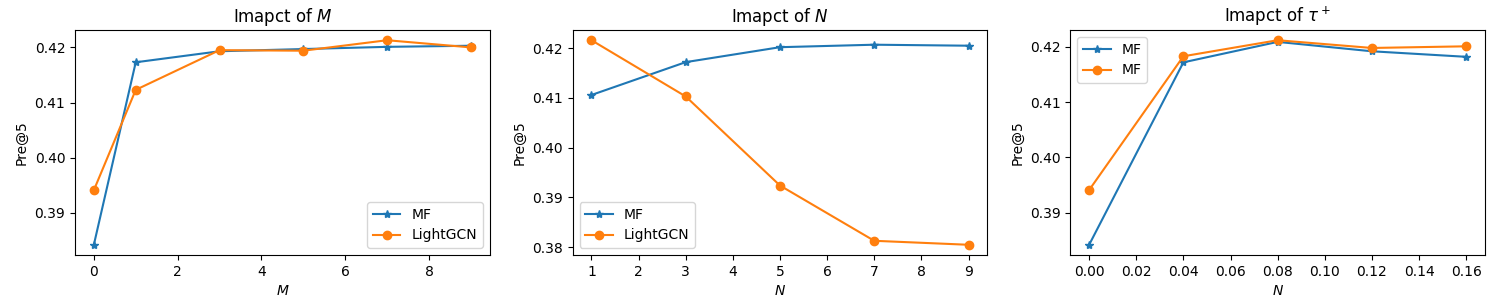
\includegraphics[width=\textwidth]{4-parameter.png}
	\caption{不同超参数的影响} %需要说明的是无偏估计,不需要m,n趋近于无穷大,这得益于在成对学习的问题设置下,一个pu构成的datapair所对应的标签情况可以被枚举。其对应的校正项目有两个正例构成,我们能refer to 图1的阐释性例子说明两个正例构成的补偿项目的由来。
	\label{Fig:parameter}
\end{figure*}
M参数的影响:参数M控制用于纠正采样偏差的额外正例数量。当M=0时,没有去偏机制。对于MF模型,较大的M和N通常会导致性能提升,从M=0到M=1观察到显著的性能提升,突出了使用额外正例进行去偏的重要性。然而,当M和N超过一个小的常数时,性能不再提高。这是因为进一步增加M和N所带来的估计准确性的边际收益变得有限,正如之前的理论分析所述。

N参数的影响:参数N控制用于计算PU概率的负例数量。与MF模型类似,增加M始终会提高LightGCN的性能。然而,当负例数量N增加时,模型性能意外地下降。这个非预期的结果可能应该归因于较大的N会降低难负例样本的梯度值。根据詹森不等式,$-\log(\frac{1}{N} \sum_{i=1}^N P_n) \leq -\frac{1}{N} \sum_{i=1}^N \log P_n $;因此,过高的N值削弱了难负样本对学习算法的贡献。理论分析假设得分$g(\cdot)$是独立同分布(i.i.d.)变量,并且估计误差随着N的增加而减小。然而,基于图神经网络编码器的聚合机制严重影响了$g(\cdot)$值的独立同分布性质。因此,当推荐模型为难以优化的神经网络模型如LightGCN时,应当设置较小的N值。

正类先验$\tau^+$的影响:随着$\tau^+$增加,MF和LightGCN模型的性能呈现出倒U型曲线,先增加后减少。这是因为设置过低或过高的$\tau^+$值可能导致公式\eqref{eq:est}的估计结果偏倚。一种常见的设置$\tau^+$值的方法是将观察到的正交互作用的数量$|\mathcal{D}^+|$视为伯努利试验的结果,该试验总共发生$|\mathcal{U}|\times |\mathcal{I}|$次,成功的次数为观察到的交互作用数量。数据集的密度$|\mathcal{D}^+|/(|\mathcal{U}|\times |\mathcal{I}|)$可以作为设置$\tau^+$值的参考。然而,需要注意的是,基于数据集密度设置的$\tau^+$值也是一种偏倚估计,低估了真实值,因为数据中的所有未观察到的(u, i)对都被视为负样本,导致成功次数的低估。详细讨论可参考~\cite{Jain:2016:NIPS,Christoffel:2016:ACML}。

\subsubsection{估计校正 vs 负采样}
负采样和估计校正代表了解决采样偏差问题的两种不同技术方法。负采样的核心思想是在模型外选择理想的样本并将其喂入模型训练,而估计校正的思想是使用随机样本,但对损失函数进行修正。从贝叶斯统计的角度来看,负采样利用了两种类型的信息:先验信息,如物品类别和流行度,这是静态的信息,用于采样用户不喜欢的负样本;样本信息,如分数和排名位置,这是动态的信息,在模型训练过程中不断调整,并用于采样嵌入接近锚点嵌入(得分较高)的难样本。各种负采样算法之间的差异在于它们如何利用和处理这两种类型的信息。上一章的贝叶斯负采样算法制定了后验概率意义上的负信号测度,并提出了理论上最优的采样规则。表~\ref{Table:vsns}中比较了DPL和BNS的性能。
\begin{table*}[h!]
	\centering
	\caption{去偏成对学习算法与负采样算法的性能比较}\label{Table:vsns}
	\resizebox{1\textwidth}{!}{
		\begin{tabular}{lllccccccccccc}
			\toprule[1.2pt]
			\multirow{2}*{\textbf{数据集}} & \multirow{2}*{\textbf{模型}} & \multirow{2}*{\textbf{方法}} & \multicolumn{3}{c}{Top-5} &~& \multicolumn{3}{c}{Top-10}&~&\multicolumn{3}{c}{Top-20}\\ \cline{4-6} \cline{8-10} \cline{12-14}
			~ & ~ & ~ & Precision& Recall& NDCG& ~ &Precision& Recall& NDCG& ~ &Precision& Recall& NDCG \\ \hline
			
			\multirow{4}*{\textbf{MovieLens-100k}} & \multirow{4}*{\textbf{MF}} & BPR & 0.3900   &0.1301	&0.4143	&~&0.3363	&0.2164	&0.3967& ~&0.2724&0.3298&0.3962 \\
			~ & ~ &BNS   &0.4205 &0.1467	&0.4558&~	&0.3463	&0.2290	&0.4217& ~&0.2762&0.3466& 0.4176\\	
			~ & ~ &DPL(Proposed)    &0.4348 & 0.1523 & 0.4643 & ~ & 0.3635 & 0.2379 & 0.4356 & ~ & 0.2914 & 0.3588 & 0.4338 \\
			~ & ~ &DPL with Hard Samples   &0.4401 & 0.1579 & 0.4692 & ~ & 0.3713 & 0.2407 & 0.4395 & ~ & 0.2940 & 0.3592 & 0.4351 \\\hline \hline 
			
			
			\multirow{4}*{\textbf{MovieLens-1M}} & \multirow{4}*{\textbf{MF}} & BPR &0.3843    &0.0855	&0.4027	&~&0.3353	&0.1430	&0.3737& ~&0.2798&0.2244&0.3572\\ 
			~ & ~ & BNS&0.4207	&0.1062	&0.4324&~	&0.3518	&0.1703	&0.4191& ~&0.3045&0.2614&0.4002 \\
			~ & ~ & DPL(proposed) & 0.4212 & 0.0998 & 0.4407 & ~ & 0.3624 & 0.1625 & 0.4071 & ~ & 0.2991 & 0.2518 & 0.3891  \\
			~ & ~ & DPL with Hard Samples & 0.4251 & 0.1012 & 0.4412 & ~ & 0.3649 & 0.1701 & 0.4151 & ~ & 0.3012 & 0.2539 & 0.3922  \\\hline 
			\bottomrule[1.5pt]
		\end{tabular}
	}
\end{table*}
\begin{figure}[h!]
	\centering
	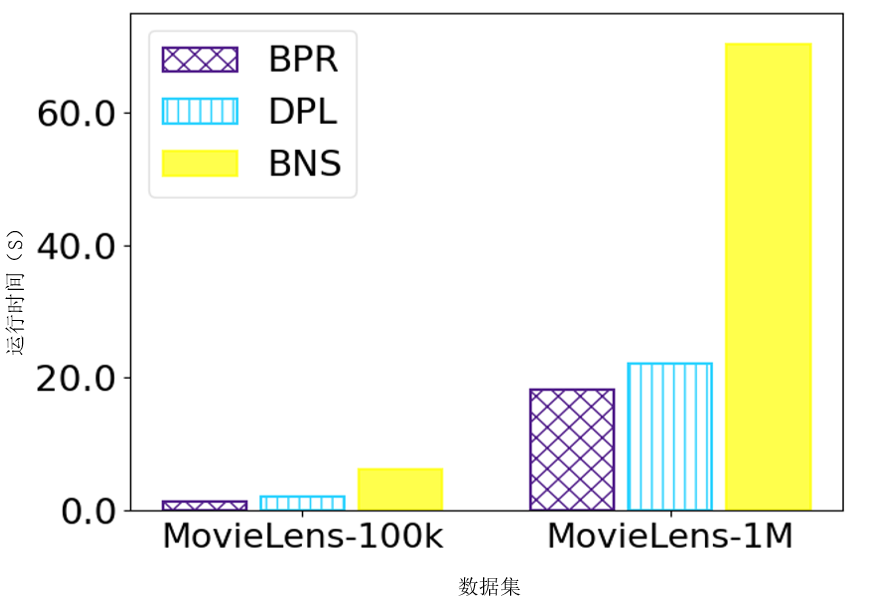
\includegraphics[width=0.6\textwidth]{4-runtime.png}
	\caption{去偏成对学习算法和负采样算法的运行时间比较} %需要说明的是无偏估计,不需要m,n趋近于无穷大,这得益于在成对学习的问题设置下,一个pu构成的datapair所对应的标签情况可以被枚举。其对应的校正项目有两个正例构成,我们能refer to 图1的阐释性例子说明两个正例构成的补偿项目的由来。
	\label{Fig:runtime}
\end{figure}

\textit{性能比较}:
DPL在MovieLens100k数据集上取得了更好的性能,并且在MovieLens1M数据集上与BNS表现相似,这表明基于校正估计的DPL作为一种替代负采样算法是可行的。此外,我们发现使用困难、得分较高的未标记样本来训练DPL可以带来一些性能改进。当使用困难样本训练DPL时,需要设置相对较大的$\tau^+$值。在表~\ref{Table:vsns}中,分别将$\tau^+$设置为0.3和0.25,这比数据集本身的密度要高得多。这是因为使用困难样本训练DPL会增加模型遇到误分类负样本的概率,这相当于人为地改变了喂入模型的训练样本的正类先验。

\textit{运行时间}: 运行时间是在一台配备2.1 GHz CPU、RTX 1080Ti GPU和32 GB RAM的个人计算机上进行测试的。图~\ref{Fig:runtime}显示了三种算法在五个数据集上进行一次epoch训练的运行时间,其中协同过滤模型固定为MF,批大小固定为1024。在计算经验分布函数时,BNS只采用mini-batch内的样本近似计算。如图~\ref{Fig:runtime}所示,DPL的实际运行时间仅略长于BPR,这与之前的时间复杂性分析一致。即使采用批内样本近似以节省计算成本,BNS的运行时间仍然是BPR和DPL的3-5倍。这是因为动态负采样需要预测得分来指导负采样,但基于GPU的批计算在进行前向传播以预测得分之前需要固定的负样本。因此,动态负采样通常通过将额外的负样本作为候选项加载到小批量数据中来实现,从而导致额外的计算成本。此外,一些最先进的动态负采样算法在前几个训练epoch中需要样本的排名位置或预测得分的方差~\cite{Ding:2019:NeurIPS},这要求模型在进行前向传播时计算整个用户-物品评分矩阵的预测得分,而不仅仅是小批量数据内的得分,从而导致指数级的时间复杂度。

总之,在具有丰富的辅助信息的场景中,建议使用可以灵活组合先验信息和模型信息的负采样算法。在没有可用的辅助信息进行监督的场景中,建议使用DPL方法进行损失修正。
\section{本章小结}
本章专注于解决来自正样本-未标记隐性反馈数据的采样偏差问题,但采用了与显式的负采样不同的技术方法。具体而言,本章提出了一种用于隐性反馈采样偏差的估计校正方法,从而为成对学习提供了一种修正的损失函数,称为去偏对数损失(DPL)。DPL的关键思想是纠正由伪负例导致的概率估计偏差,从而修正梯度以近似完全监督数据的梯度。所提出的目标函数易于实现,不需要额外的辅助信息进行监督,也不需要过多的存储和计算开销。在保持严格的相对于BPR的线性时间复杂度情况下,DPL取得了相对于负采样相当或更优的表现。

式\eqref{eq:infonce1}展示了成对损失和对比损失的联系,成对损失函数是负例个数N=1的对比损失的特例。本章聚焦于成对损失的去偏研究,DPL的去偏机制的核心可以参考图~\ref{fig:event},在只有一个负例的情况下,未标注样本的真实标签有且只有两种可能性,很容易被枚举出来。在自监督对比学习中,一个广泛的共识是负例个数N越大,学到的对比表示在下游任务中泛化表现越好\cite{Oord:2018:arxiv,Chuang:2020:NIPS,Robinson:2021:ICLR},这是由于更大的N推高了已知数据和待预测数据互信息的下界。但是,随着未标注样本N的增长,真实的标签的可能性指数级增长为$2^N$种,难以被枚举出来,导致本章的去偏思路则难以向更大的负例数推广。那么如何将去偏差的方法向更一般的对比损失推广?此外,对于在自监督对比学习任务而言,除了去偏以防止伪负例被推远,还有一个重要的硬负例挖掘任务,使真负例被推远。本章只考虑到前者。如何同时兼顾伪负例去偏和硬负例挖掘任务?下一个章节将针对这两个问题给出解决方案。


\chapter{对比损失函数校正研究}
\label{cha:fifthsection}



\label{sec:parameters}
在对比学习种,负例个数N推高了已知数据和待预测数据互信息的下界,使得学到的对比表示在下游任务中泛化表现越好\cite{Oord:2018:arxiv,Chuang:2020:NIPS,Robinson:2021:ICLR}。然而随着未标注样本N的增长,真实的标签的可能性指数级增长为$2^N$种,难以被枚举出来,导致上一章的去偏思路难以向更大的负例数推广;此外,对于在自监督对比学习任务而言,一方面要考虑伪负例去偏以防止伪负例被推远,另一方面还要考虑硬负例挖掘任务,使真负例被推远。本章聚焦于负例个数大于1的更一般的自监督对比学习的去偏差任务,并且进一步将硬负例挖掘任务纳入考量,通过引入重要性权重校正未标注样本的权重,得到了一种校正后的对比损失函数,称为贝叶斯自监督对比学习损失(Bayesian self-supervised contrastive loss, BCL)。从损失函数的数值来看,BCL提供了完全监督数据下对比损失函数的渐进一致估计;从单个重要性权重来看,BCL提供了未标注样本是真负样本的后验概率估计。在数值实验,四个公图像数据集,以及五个推荐数据集进行的实验研究验证了所提出的学习方法的有效性。

\section{引言}
无监督学习因为不依赖人工标注数据而广受关注。然而,在没有监督信号的情况下学习,如何到良好的表示一直是机器学习领域面临的一个长期挑战。最近,对比学习(contrastive learning)作为一种有希望的解决方案被提出,通过利用对比损失(contrastive loss)来训练表示编码器,从而改善无监督学习的表示能力。对比学习已经在各个领域展现出显著的成功,并且在计算机视觉、自然语言处理和推荐系统等任务中得到广泛应用,甚至在部分任务上超过了传统的有监督学习方法。

对比学习采用从比较种学习(learn-to-compare)的范式~\cite{Gutmann:2010:ICAIS},通过区分观察数据和噪声数据来使模型免于重建数据的像素级信息~\cite{Oord:2018:arxiv}。虽然表示编码器$f$和相似性度量会因任务而异~\cite{Devlin:2018:bert,He:2020:CVPR,Dosovitskiy:2014:NIPS},但它们都共享一个将相似对$(x, x^+)$和不相似对$(x, x^-)$进行对比的基本思想,通过优化对比损失~\cite{Wang:2020:ICML}来训练$f$,如NCE损失~\cite{Gutmann:2010:ICAIS},InfoNCE损失~\cite{Oord:2018:arxiv},Infomax损失~\cite{Hjelm:2018:Arxiv},渐进对比损失~\cite{Wang:2020:ICML}等。这些损失函数隐式~\cite{Oord:2018:arxiv}或显式~\cite{Hjelm:2018:Arxiv}地优化了已知数据和待预测数据的互信息下界。Arora等人~\cite{Saunshi:2019:ICML}为分类任务的对比学习的泛化界限提供了理论分析。在不同领域的许多应用中都观察到了监督对比学习的显著成功~\cite{Henaff:2020:ICML,Khosla:2020:NIPS},但其主要局限性来自于对手动标注数据集的依赖~\cite{Liu:2021:TKDE}。自监督对比学习~\cite{Chen:2020:ICML,Chen:2020:NIPS,He:2020:CVPR,Henaff:2020:ICML, Xu:2022:Arxiv}可以看作无监督学习的一个分支,它能够在无需人工标注数据的情况下学习表示,并且利益几乎所有类型的下游任务~\cite{Liu:2021:TKDE,Bachman:2019:NIPS,chen2020improved,Huang:2019:ICML,Wu:2018:CVPR,Zhuang:2019:CVPR}。

然而,当前的自监督对比学习仍存在一些挑战和局限性,主要还是由于无监督或者弱监督引发的positive-unlabeled问题。通常的做法是通过在锚点$x$上进行某些语义不变的数据增强~\cite{Chen:2020:ICML}来获得正样本$x^+$,如随机裁剪和翻转~\cite{Oord:2018:arxiv},图像旋转~\cite{Komodakis:2018:ICLR},和颜色失真~\cite{Szegedy:2015:CVPR}等;而负样本$x^-$则简单地从未标签数据中抽取,从而构成了positive-unlabeled问题。特别是,自监督对比学习面临两个冲突的任务~\cite{Liu:2021:TKDE,Robinson:2021:ICLR}:伪负样本的偏差修正和真负样本的硬负例挖掘。本章聚焦于更一般的自监督对比学习的去偏差任务,并且综合考虑了去偏任务和硬负例挖掘任务,称为贝叶斯自监督对比学习损失(Bayesian self-supervised contrastive loss, BCL)。BCL利用重要性权重来纠正使用从未标记数据中随机抽取的负样本所带来的偏差,提供了完全监督数据下对比损失函数的渐进一致估计,以及未标注样本是真负样本的后验概率估计,为去偏任务和硬负例挖掘任务提供了灵活统一的框架。

\section{对比损失优化目标分析}
CPC~\cite{Oord:2018:arxiv}提出了在自监督对比学习中广泛使用的InfoNCE损失,并构建了InfoNCE损失的优化与互信息优化的联系。在理想的监督信息下,优化InfoNCE损失会导致优化已知数据和待预测数据的互信息下界,免于迫使编码器重建样本的像素级信息。然而,在负例未标注的情况下,本节将说明优化InfoNCE损失会导致另外一种不同的结果,即,互信息下界的不可控优化。本小节的内容主要是分析负例未标注时,有偏的对比损失与互信息优化的理论关联,阅读与否不影响对后面的算法内容理解。

在有监督对比学习(supervised contrastive learning)的背景下,可以通过随机抽取与锚点不同类的真负例$x^-\sim p^-$来轻松构建不相似的样本对$(x,x^-)$,通过优化如下有监督的损失
\begin{equation}\label{Eq:SupLoss}
	\small
	\mathcal{L}_\textsc{Sup} = \mathbb E_{\substack{x \sim p_d\\~x^+ \sim p^+\\\color{blue}{~x^- \sim p^-}} }
	[-\log \frac{e^{f(x)^Tf(x^+)}}{e^{f(x)^Tf(x^+)} + \sum_{i=1}^Ne^{f(x)^Tf(x_i^-)}}]
\end{equation}
以训练一个编码器$f: \mathcal{X} \rightarrow \mathbb{R}^d/t$,该编码器将数据点$x$映射到半径为$1/t$的超球面$\mathbb{R}^d$上,其中$t$是温度缩放参数。本章中,在理论分析中也将$t$设为1以简化分析。

然而,在自监督对比学习(self-supervised contrastive learning)的场景下,由于样本的标签不可得,无法获得真负例的类条件概率分布$x^- \sim p^-$,标准方法是从数据分布$p_d$中抽取$N$个样本,这些样本被假设为$x$的负样本,以优化以下的InfoNCE损失:
\begin{equation}\label{Eq:BiasLoss}
	\small
	\mathcal{L}_\textsc{Biased}= \mathbb E_{ \substack{x \sim p_d\\~x^+ \sim p^+\\\color{blue}{~x^\prime \sim p_d}}}
	[-\log \frac{e^{f(x)^Tf(x^+)}}{e^{f(x)^Tf(x^+)} + \sum_{i=1}^{N}e^{f(x)^Tf(x_i^\prime)}}].
\end{equation}
这也被称为“有偏对比损失”~\cite{Chuang:2020:NIPS},因为从$p_d$中抽取的那些随机未标注样本$x^\prime$,它是伪负例(正例)的概率为$\tau^+$。

依照前文的符号标记,记$x^\prime\in \textsc{Tn}$表示$x^-$是相对于锚点数据$x$的真负例(TN)样本,记$x^\prime\in \textsc{Fn}$表示$x^\prime$是相对于锚点$x$的伪负例(FN)样本,记$\hat{x}^+=e^{f(x)^Tf(x^+)}$,表示正例和锚点的相似度得分。注意,$x^\prime$是TN还是FN是针对特定的锚点$x$而言的,在接下来的讨论中,为简洁起见,本章省略了正负样本是“相关于锚点$x$”的概念表述。已经证明,对于$\{x_i^\prime \in \textsc{Tn} \}_{i=1}^N$,优化完全监督的InfoNCE损失(式\eqref{Eq:SupLoss})将导致正例的相似度分数正比于密度比$\frac{p^+}{p^-}$\cite{Oord:2018:arxiv,Ben:2019:ICML}
\begin{equation}\label{Eq:LsupDensityRatio}
	\hat{x}^+ \propto p^+/p^-.
\end{equation}
互信息的最大化是科学和工程中的一个基本问题~\cite{Ben:2019:ICML,Belghazi:2018:ICML},密度比$p^+/p^-$保存了未来信息和当前信号的互信息(MI)。为了使式~\eqref{Eq:SupLoss}最小化,模型优化使得正例的相似度得分增加,从而使得密度比$p^+/p^-$增加,间接地实现最大化互信息。

现在考虑式~\eqref{Eq:BiasLoss}中从未标注样本中采样的InfoNCE损失$\mathcal{L}_\textsc{Biased}$,它的含义是从N个未标记样本中分类出一个正样本的交叉熵。为了便于分析,将$x^+$记为$x_0$。给定$N+1$个样本,可以通过以下方式推导出一个数据点$x_0$是正样本的后验概率:
\begin{eqnarray}
	P(x_0\in \textrm{pos}| \{x_i\}_{i=0} ^N) 
	&=& \frac{p^+(x_0) \prod_{i=1}^{N} p_d(x_i)}{\sum_{j=0}^{N} p^+(x_j) \prod_{i \neq j} p_d (x_i)} \nonumber \\
	&=& \frac{p^+(x_0)/p_d(x_0)}{p^+(x_0)/p_d(x_0) + \sum_{j=1}^{N} p^+(x_j)/p_d(x_j)}
\end{eqnarray}

最小的损失值$\mathcal{L}_\textsc{Biased}$在后验概率为1时取到,通过密度比取如下极限实现$p^+(x_0)/p_d(x_0) \rightarrow +\infty$或$p^+(x_j)/p_d(x_j)\rightarrow 0$。于是,最小化$\mathcal{L}_\textsc{Biased}$导致正例分数正比于正例和未标注数据的密度比
\begin{eqnarray}\label{eq:propoto}
	\hat{x}^+ \propto p^+/p_d.
\end{eqnarray}
需要注意的是,这与公式~\eqref{Eq:LsupDensityRatio}是不同的,前者是正例与负例的密度比,后者是正例与未标注样本的密度比。记$\hat{x}^+ = m\cdot p^+/p_d, m \ge 0$。下面探讨优化$\hat{x}^+$和优化目标$p^+/p^-$之间的差距。将全概率公式$p_d = p^-\tau^-+ p^+\tau^+$代入公式\eqref{eq:propoto},有
\begin{eqnarray} \label{eq:gap}
	\hat{x}^+ = m\cdot \frac{p^+}{p^-\tau^-+ p^+\tau^+}.
\end{eqnarray}
整理上式,有
\begin{equation}\label{eq:fractional}
	p^+/p^- = \frac{\hat{x}^+ \cdot \tau^-}{m-\hat{x}^+ \cdot \tau^+}.
\end{equation}
\par

图~\ref{Fig:gap}展示了公式~\eqref{eq:fractional}作为分数函数的近似形状,揭示了使用PU数据时,InfoNCE $\mathcal{L}_\textsc{Biased}$损失优化和互信息(MI)优化之间的不一致性。也就是说,在使用PU数据优化InfoNCE损失时,增加$\hat{x}^+$并不会导致$p^+/p^-$的单调增加。跳跃间断点的存在表明,$\mathcal{L}_\textsc{Biased}$的优化不一定会导致可控的MI优化。MI优化的难题源于以下事实:并非所有的$\{x_i^\prime\}_{i=1}^N$都是$\textsc{Tn}$样本,因为它们是从数据分布$ p_d $中随机抽取的。这导致在分解数据分布$ p_d $时,公式~\eqref{eq:gap}的分母中包含了$ p^+$。图~\ref{Fig:illustrative}提供了直观的解释。这五个随机抽样的样本实际上包含一个伪负例$\textsc{Fn}$样本。这样的伪负样本应该被拉近到锚点$x$附近。然而,由于它被错误地当作负样本时,在模型训练过程中,它将被推离锚点,这破坏了嵌入表示的语义结构~\cite{Feng:2021:CVPR}。
\begin{figure}[!]
	\centering
	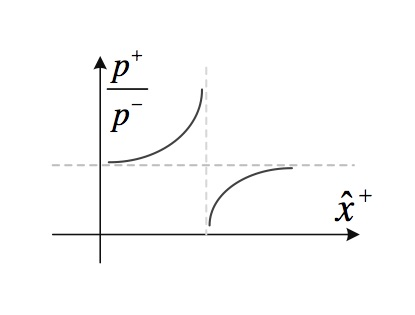
\includegraphics[scale=0.5]{gap.jpeg}
	\caption{有偏对比损失与互信息优化示意图}
	\label{Fig:gap}
\end{figure}


\section{贝叶斯自监督对比学习算法}
\subsection{伪负例去偏与硬负例挖掘}\label{subsec:fh}
%*******************************
\begin{figure*}[!]
	\centering
	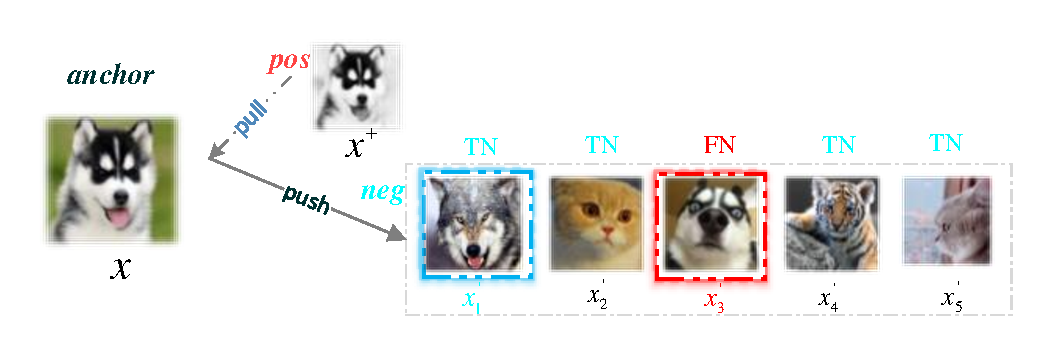
\includegraphics[width=0.9\textwidth]{pucon.pdf}
	\caption{自监督对比学习的伪负例去偏和硬负例挖掘示意图}
	\label{Fig:illustrative}
\end{figure*}
%*******************************
本小节使用图像的例子来阐释自监督对比学习中的最重要两个任务:伪负例去偏和硬负例挖掘。对于一个锚点为“狗”的图像,正例通过语义不变的图像增强获得,负例从未标记图像中随机抽样,假设共得到五个随机负样本$\{x_1^\prime,x_2^\prime,x_3^\prime,x_4^\prime,x_5^\prime\}$。其中$x_3^\prime$的真实标签是“狗”,是与锚点同类的伪负例(FN)。剩余4个随机负样本是与锚点不同类的真负例(TN),其中$x_1^\prime$的真实标签与锚点不同类的“狼”,但是它与锚点很相似难以区分,称为困难负样本(hard negative sample)。

对比学习的任务是拉近正样本,推远负样本。由于随机负样本可能是真负例或者伪负例,那么根据未标注样本的标签不同,就存在两个不同的考量:
\begin{itemize}
\item \textit{伪负例去偏}:对于与锚点同类的伪负例$x_3^\prime$,应当防止它被推离锚点,保持“狗”这个类的样本距离比较近,也称为对齐(alignment)。
\item \textit{硬负例挖掘}:对于与锚点不同类的真负例$x_1^\prime$,应当把它推远离锚点,保持“狗”和“狼”这两个类之间的样本距离比较远,也称为均匀(uniformity)。
\end{itemize}

这个例子也可以类比在推荐系统中,略微的差异是锚点的选择,图像中任意样本都可以做锚点,而在推荐系统中通常只有用户才会作为锚点。推荐系统中的正例是从观测到的交互中获得,负例是从未交互的物品中随机抽样获得。根据未标注样本标签的不同,同样也面临着上述硬负例挖掘和伪负例去偏的任务。

考虑$\{x_1^\prime,x_2^\prime,x_3^\prime,x_4^\prime,x_5^\prime\}$的标签,每个标签只有两种可能:与锚点类型不同时为真负例,与锚点类型相同时为伪负例。根据二项式定理,五个未标注样本的真实标签共有$2^5=32$种可能的情况。当N很大时,枚举每一种情况,并对每一种情况进行极大似然估计是非常困难的,上一章的思想难以向较大负例个数N推广。受到经典的重要性采样(importance sampling)技术的启发,可以在每个未标注样本$x_i^\prime$添加一个重要性权重$\omega_i$,以纠正未标记样本中抽取负样本所产生的偏差。那么包含重要性权重的对比损失函数可以重写为
\begin{eqnarray}
	\small
	\mathcal{L} &=& \mathbb E_{ \substack{x \sim p_d\\~x^+ \sim p^+\\{~x^\prime \sim p_d}}}
	[-\log \frac{e^{f(x)^Tf(x^+)}}{e^{f(x)^Tf(x^+)} + \sum_{i=1}^{N} \omega_i \cdot e^{f(x)^Tf(x_i^\prime)}}] \nonumber \\
	&=& \mathbb E_{ \substack{x \sim p_d\\~x^+ \sim p^+\\{~x^\prime \sim p_d}}}
	[-\log \frac{\hat{x}^+}{{\hat{x}^+} + \sum_{i=1}^{N} \omega_i \cdot \hat{x}_i}] \label{eq:debias}
\end{eqnarray}
式~\eqref{eq:debias}是把正例与锚点的相似度得分$e^{f(x)^Tf(x^+)}$记为$\hat{x}^+$,把负例(实际上是未标注样本)与锚点的相似度得分$e^{f(x)^Tf(x^\prime)}$记为$\hat{x}$,以保持分析过程中符号的简洁性。
		
下面考察在包含重要性权重后,权重$\omega_i$是如何控制未标记样本$x^\prime_i$对模型的参数学习与更新。损失函数相对于模型的参数$\Theta$的梯度可以计算为:
\begin{eqnarray}
\frac{\partial\mathcal{L}}{\partial \Theta} &=& \frac{\partial\mathcal{L}}{\partial \hat{x}_i^\prime} \cdot \frac{\partial \hat{x}_i}{\partial\Theta} \\
&=&  \frac{ \omega_i\hat{x}_i} {\hat{x}^+ + \sum_{i=1}^{N} \omega_i \cdot \hat{x}_i}\cdot \frac{\partial \hat{x}_i}{\partial\Theta} \label{eq:rule}
\end{eqnarray}
式~\eqref{eq:rule}是微分的链式法则的结果,第一项$\frac{ \omega_i\hat{x}_i} {\hat{x}^+ + \sum_{i=1}^{N} \omega_i \cdot \hat{x}_i}$由损失函数的具体形式决定的,第二项$ \frac{\partial \hat{x}_i}{\partial\Theta}$由编码器和评分函数的形式决定的。可以看到,重要性权重$\omega_i$出现在第一项的分子,作用类似一个调节器,它直接控制了未标注样本$x_i^\prime$对模型参数更新的贡献大小,进而控制了这些样本被推多远。

从正例对齐、负例均匀的任务目标考虑,合意的权重$\omega_i$应该满足如下要求:
\begin{itemize}
\item 如果未标注样本$x_i^\prime$是一个和锚点同类的伪负例,合意的权重$\omega_i$应该取值较小,最好是0,以防止正样本被推远,使得同类样本距离较近,体现\textit{伪负例去偏原则}。伪负例可以看作负样本中出现的噪声,较小的$\omega_i$可以使得式~\eqref{eq:rule}的梯度消失,能够防止模型学到噪声样本的模式。
\item 如果未标注样本$x_i^\prime$是一个和锚点不同类的真负例,合意的权重$\omega_i$应该取值较大,以推远硬负样本,使得不同类样本距离较远,体现\textit{硬负例挖掘原则}。困难负样本可以看作难以拟合的负样本,较大的$\omega_i$可以使得式~\eqref{eq:rule}的梯度幅度增加,激励模型去学习难以区分的样本之间的决策边界。
\end{itemize}

综合上面的分析,合意的$\omega_i$与相应的未标注样本$x^\prime_i$的所属类别相联系:\textit{未标注样本$x^\prime_i$是真负例的概率越低,权重$\omega_i$值应该越小(伪负例去偏要求);未标注样本$x^\prime_i$是真负例的概率越高,权重$\omega_i$应该越大(硬负例挖掘要求)}。下面章节将介绍如何计算一个合意的重要性权重,满足上述要求。

\subsection{重要性权重计算}
\subsubsection{相似度分数分布}
根据重要性采样的规定步骤,需要目标抽样群体的硬负例的分布,和实际抽样群体的未标注样本的分布,那么重要权重为目标抽样群体和实际抽样群体分布的密度比。为了得到这个权重,首先聚焦于未标注样本与锚点的相似度分数$\hat{x}$,它更一般的形式化表示方式为$\exp(\text{sim}(f(x),f(x^\prime))/t)$,其中$f(\cdot)$是基于深度神经网络的编码器编码的表示向量,$\text{sim}(f(x),f(x^\prime))$表示锚点嵌入和未标记样本嵌入的相似度,如内积余弦相似度等。$t$为温度系数。

视未标注样本$x^\prime$为随机变量,则相似度分数$\hat{x} = \exp(\text{sim}(f(x),f(x^\prime))/t)$的分布的影响因素众多:与锚点$x$的选择有关,与神经网络$f(\cdot)$的结构有关,也与相似度函数$\text{sim}(\cdot,\cdot)$的具体形式有关。第\ref{cha:2}章的引理~\ref{Lemma2:AprioriDistribution}讨论了,在取似度函数$\text{sim}(\cdot,\cdot)$为向量内积时,即使是简单的两个高斯随机向量的相似度,其分布表达式也是非常复杂的,经过非线性函数$\exp(\cdot/t)$映射以后,想获取其密度表达式更加困难。况且,假设基于深度神经网络学到的表示向量$f(x)$服从高斯分布也及其牵强。因此,第\ref{cha:2}章的方法,以及现有的研究\cite{Xia:2022:ICML}通过高斯混合模型\cite{Lindsay:1995}、Beta混合模型~\cite{Xia:2022:ICML}等参数化方法来拟合未标注样本的相似度分数$\hat{x}$分布,引入了过强的假设,不具一般性。此外,用于密度估计的学习算法是昂贵的,因为混合系数是隐藏变量,只能通过EM算法~\cite{Dempster:1977:RSS}的迭代数值计算来获得,且算法对初始值非常敏感。

本节提出了一种方法,无需显式地估计相似度分数分布,即可实现对密度比的解析计算。对于固定的锚点,假设该锚点与其他未标注样本的相似度分数$\hat{x}$独立同分布于某个锚点特定的未知分布$\phi$,即
\begin{eqnarray}
\hat{x} \sim \phi(\hat{x})
\end{eqnarray}
相应的累积分布函数$\Phi(\hat{x})=\int_{-\infty}^{\hat{x}} \phi(t) dt$。注意,分布$\phi$是特定于锚点的,不同锚点对应的相似度分数分布不必相同。由于不对分布$\phi$做出任何假设,因此本方法属于非参数方法。根据上述抽象表达式,可以写出它对应的次序统计量分布为:
\begin{eqnarray}
	\phi_{(1)}(\hat{x}) &=& 2\phi(\hat{x}) [1-\Phi(\hat{x})] \label{eq:order1} \\
	\phi_{(2)}(\hat{x}) &=& 2\phi(\hat{x}) \Phi(\hat{x}) \label{eq:order2}
\end{eqnarray}

\subsubsection{目标采样群体}
对于固定的锚点$x$,若随机样本是伪负例$x^\prime\in \textsc{Fn}$,则记该未标注样本与锚点的相似度分数$\hat{x} \in \textsc{Fn}$,表明这是一个来自伪负例的相似度分数,所有的伪负例相似度分数总体对应的类条件概率密度记为$\phi_\textsc{Fn}$。类似地,若随机样本是真负例$x^\prime\in \textsc{Tn}$,则记该未标注样本与锚点的相似度分数$\hat{x} \in \textsc{Tn}$,表明这是一个来自伪负例的相似度预测分数,所有的真负例相似度分数总体的类条件概率密度记为$\phi_\textsc{Fn}$。

接下来,可以通过正样本和负样本的表示在超球面上的相对位置,解析真负例的类条件概率密度$\phi_{\textsc{Tn}}$表达式。考虑一个锚点,正例和真负例构成的$(x, x^+, x^-)$三元组,存在一个以$ f(x) $为中心、半径为$ d^+ $的闭球$ \mathfrak{B}[f(x),d^+] =\{f(\cdot)| d(f(x),f(\cdot)) \leq d^+ \}$,其中$ d^+ = \|f(x)-f(x^+)\|$是锚点嵌入$ f(x) $和正样本嵌入$ f(x^+) $之间的距离。那么,真负例的相对位置有且只有两种可能情况:$ f(x^-) \in \mathfrak{B}[f(x),d^+] $或$ f(x^-) \notin \mathfrak{B}[f(x),d^+] $。
\begin{figure}[!]
	\centering
	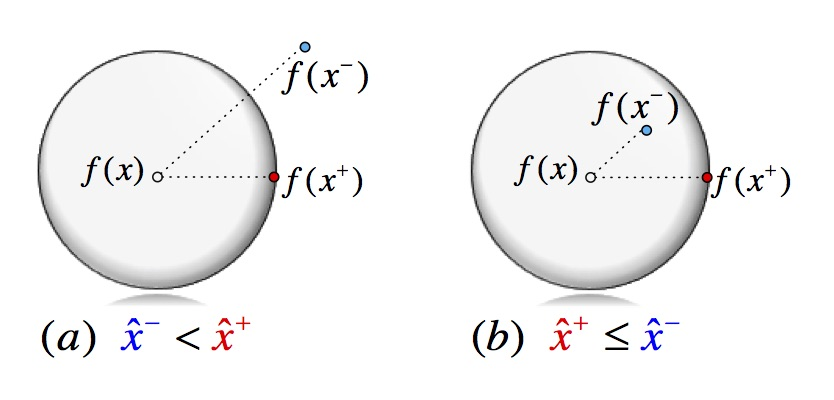
\includegraphics[scale=0.35]{openball.jpeg}
	\caption{正负样本对相对位置示意图}
	\label{Fig:openball}
\end{figure}
图~\ref{Fig:openball}描述了这两种可能的情况:图~\ref{Fig:openball}(a)对应于正例距离更近,即$ d^+ < d^- $;图~\ref{Fig:openball}(b)对应于负例距离更近,即$ d^- \leq d^+ $,其中$ d^{-}=\|f(x) - f(x^-)\|$是欧式距离度量。对于情况(a),必有$ \hat{x}^- < \hat{x}^+ $,对于情况(b),必有$ \hat{x}^+ \leq \hat{x}^- $。这是因为所有嵌入$ f(\cdot) $都在半径为$ 1/t $的超球面上,那么欧氏距离与相似度分数一一对应,存在如下关系:$ d^\pm = \sqrt{2/t^2 - 2f(x)^\mathsf{T} f(x^\pm)}$。

对于关心的真负例相似度分数$ \hat{x}^- $,在图~\ref{Fig:openball}中用蓝色进行了标记,在情况(a)下,它是次序统计量$ X_{(1)} $的一个取值,在情况(b)下是次序统计量$ X_{(2)} $的一个取值。记情况(a)发生的概率为$\alpha$,情况(b)发生的概率为$1-\alpha$。那么,真负例的相似度分数观测值的生成过程可以描述如下:以概率$\alpha$选择情况(a),然后从次序统计量分布$\phi_{(1)}$生成观测值$\hat{x}$;或者以概率$1-\alpha$选择情况(b),然后从次序统计量分布$\phi_{(2)}$生成观测值$\hat{x}$。也就是说,真负例的类条件概率密度是$\phi_{\textsc{Tn}}$是成分$\phi_{(1)}$和成分$\phi_{(2)}$以系数$\alpha$进行混合构成:
\begin{eqnarray}
	\phi_{\textsc{Tn}}(\hat{x}) = \alpha \phi_{(1)}(\hat{x}) + (1-\alpha)\phi_{(2)}(\hat{x}) \label{eq:phitn}
\end{eqnarray}

类似地,伪负例相似度分数的类条件概率密度$\phi_{\textsc{Fn}}$是成分$\phi_{(2)}$和成分$\phi_{(1)}$以系数$\alpha$进行混合构成:
\begin{eqnarray}
	\phi_{\textsc{Fn}}(\hat{x}) = \alpha \phi_{(2)}(\hat{x}) + (1-\alpha)\phi_{(1)}(\hat{x})\label{eq:phifn}
\end{eqnarray}

需要说明的是,次序统计量$X_{(1)}$的定义是满足$X_{(1)}\leq X_{(2)}$。在情况(a)下$\hat{x}^- < \hat{x}^+$,将真负例的相似度分数$\hat{x}^-$视作次序统计量$X_{(1)}$的一个取值,忽略了$\hat{x}^- = \hat{x}^+$的特殊情况。对于这种特殊情况$\hat{x}^-$的概率测度为0,因为$\phi$是由Lebesgue测度控制的连续密度函数。直观地理解,对于任意连续概率密度函数如高斯分布,随机变量取任意离散点的概率为0。下面的引理证明了,类条件概率密度$\phi_{\textsc{Tn}}$和$\phi_{\textsc{Fn}}$满足概率密度函数的非负性和归一性要求。

\begin{lemma}[类条件概率密度]
若相似度分数的分布$\phi(\hat x)$是连续的概率密度函数,满足正定性$\phi(\hat x) \geq 0 $和归一性$\int_{-\infty}^{+\infty}\phi(\hat x) d\hat x =1 $,那么

(1) $\phi_{\textsc{Tn}}(\hat{x})$是概率密度函数,满足$\phi_{\textsc{Tn}}(\hat{x})\geq 0$,且$\int_{-\infty}^{+\infty}\phi_{\textsc{Tn}}(\hat{x})d\hat x =1 $。

(2) $\phi_{\textsc{Fn}}(\hat{x})$是概率密度函数,满足 $\phi_{\textsc{Fn}}(\hat{x})\geq 0$,且  $\int_{-\infty}^{+\infty}\phi_{\textsc{Fn}}(\hat{x})d\hat x =1 $。
\begin{proof}
由于 $\phi(\hat x) \geq 0 $ 且 $\int_{-\infty}^{+\infty}\phi(\hat x) d\hat x =1 $, 因此
	\begin{eqnarray}
		\phi_{\textsc{Tn}}(\hat{x}) &=& \alpha \phi_{(1)}(\hat{x}) + (1-\alpha)\phi_{(2)}(\hat{x}) \nonumber \\ 
		&=& 2\alpha\phi(\hat{x}) [1-\Phi(\hat{x})]+ 2(1-\alpha)\phi(\hat{x}) \Phi(\hat{x}) \nonumber \\ 
		&\geq& 0,
	\end{eqnarray}
其中 $\Phi(\hat{x}) \in [0,1]$. 
	\begin{eqnarray}
		\int_{-\infty}^{+\infty}\phi_{\textsc{Tn}}(\hat{x})d\hat x &=& \int_{-\infty}^{+\infty}2\alpha\phi(\hat{x}) [1-\Phi(\hat{x})]+ 2(1-\alpha)\phi(\hat{x}) \Phi(\hat{x}) d\hat x \nonumber \\
		&=&2\alpha\int_{-\infty}^{+\infty}\phi(\hat{x}) [1-\Phi(\hat{x})] d\hat x+  2(1-\alpha)\int_{-\infty}^{+\infty} \phi(\hat{x}) \Phi(\hat{x}) d\hat x \nonumber \\
		&=&2\alpha\int_{-\infty}^{+\infty} [1-\Phi(\hat{x})] d\Phi(\hat{x}) +  2(1-\alpha)\int_{-\infty}^{+\infty}  \Phi(\hat{x}) d\Phi(\hat{x}) \nonumber \\
		&=& 2\alpha\int_{0}^{1} (1-\mu) d\mu +  2(1-\alpha)\int_{0}^{1}  \mu d\mu  \label{Eq:sub}\\
		&=& [\alpha(2\mu-\mu^2) +(1-\alpha)\mu^2] \big|_0^1 \nonumber \\
		&=&1,
	\end{eqnarray}
其中,公式~\ref{Eq:sub}是对$\Phi(\hat{x})$和$\mu$进行换元积分。同样地,
	\begin{eqnarray}
		\phi_{\textsc{Fn}}(\hat{x}) &=& \alpha \phi_{(2)}(\hat{x}) + (1-\alpha)\phi_{(1)}(\hat{x}) \nonumber\\
		&=& 2\alpha \phi(\hat{x}) \Phi(\hat{x}) +2(1-\alpha)\phi(\hat{x}) [1-\Phi(\hat{x})] \nonumber \\ 
		&\geq& 0,
	\end{eqnarray}
且
	\begin{eqnarray}
		\int_{-\infty}^{+\infty}\phi_{\textsc{Fn}}(\hat{x})d\hat x &=& 2\alpha\int_{-\infty}^{+\infty}  \phi(\hat{x}) \Phi(\hat{x})d\hat x +2(1-\alpha)\int_{-\infty}^{+\infty}\phi(\hat{x}) [1-\Phi(\hat{x})] d\hat x \nonumber \\
		&=& 2\alpha\int_{-\infty}^{+\infty} \Phi(\hat{x})d\Phi(\hat{x}) +2(1-\alpha)\int_{-\infty}^{+\infty}[1-\Phi(\hat{x})] d\Phi(\hat{x}) \nonumber \\
		&=& 2\alpha\int_{0}^{1}  \mu d\mu +2(1-\alpha)\int_{0}^{1} (1-\mu) d\mu \nonumber \\
		&=& [\alpha \mu^2 + (1-\alpha) (2\mu - \mu^2) ]\big|_0^1 \nonumber \\
		&=&1.
	\end{eqnarray}
证毕。
\end{proof}
\end{lemma}

通过查看图~\ref{Fig:openball},有助于进一步理解混合系数$\alpha$的含义:$\alpha$描述了情况(a)发生的概率,即编码器将伪负例(正例)编码到比负例更近的距离的概率,也即正例评分高于负例评分的概率。对于一个随机盲猜的最差编码器$ f $,$\alpha=0.5$;而对于一个完美的编码器$\alpha=1$。因此,合理的$\alpha$值应在$[0.5, 1]$范围内。实际上,$\alpha$的含义就是当前训练时点的编码器的AUC,它对应于数据集$\mathcal{D}$中所有锚点$ x $宏平均的AUC经验估计:
%*******************************
\begin{figure}[!]
	\centering
	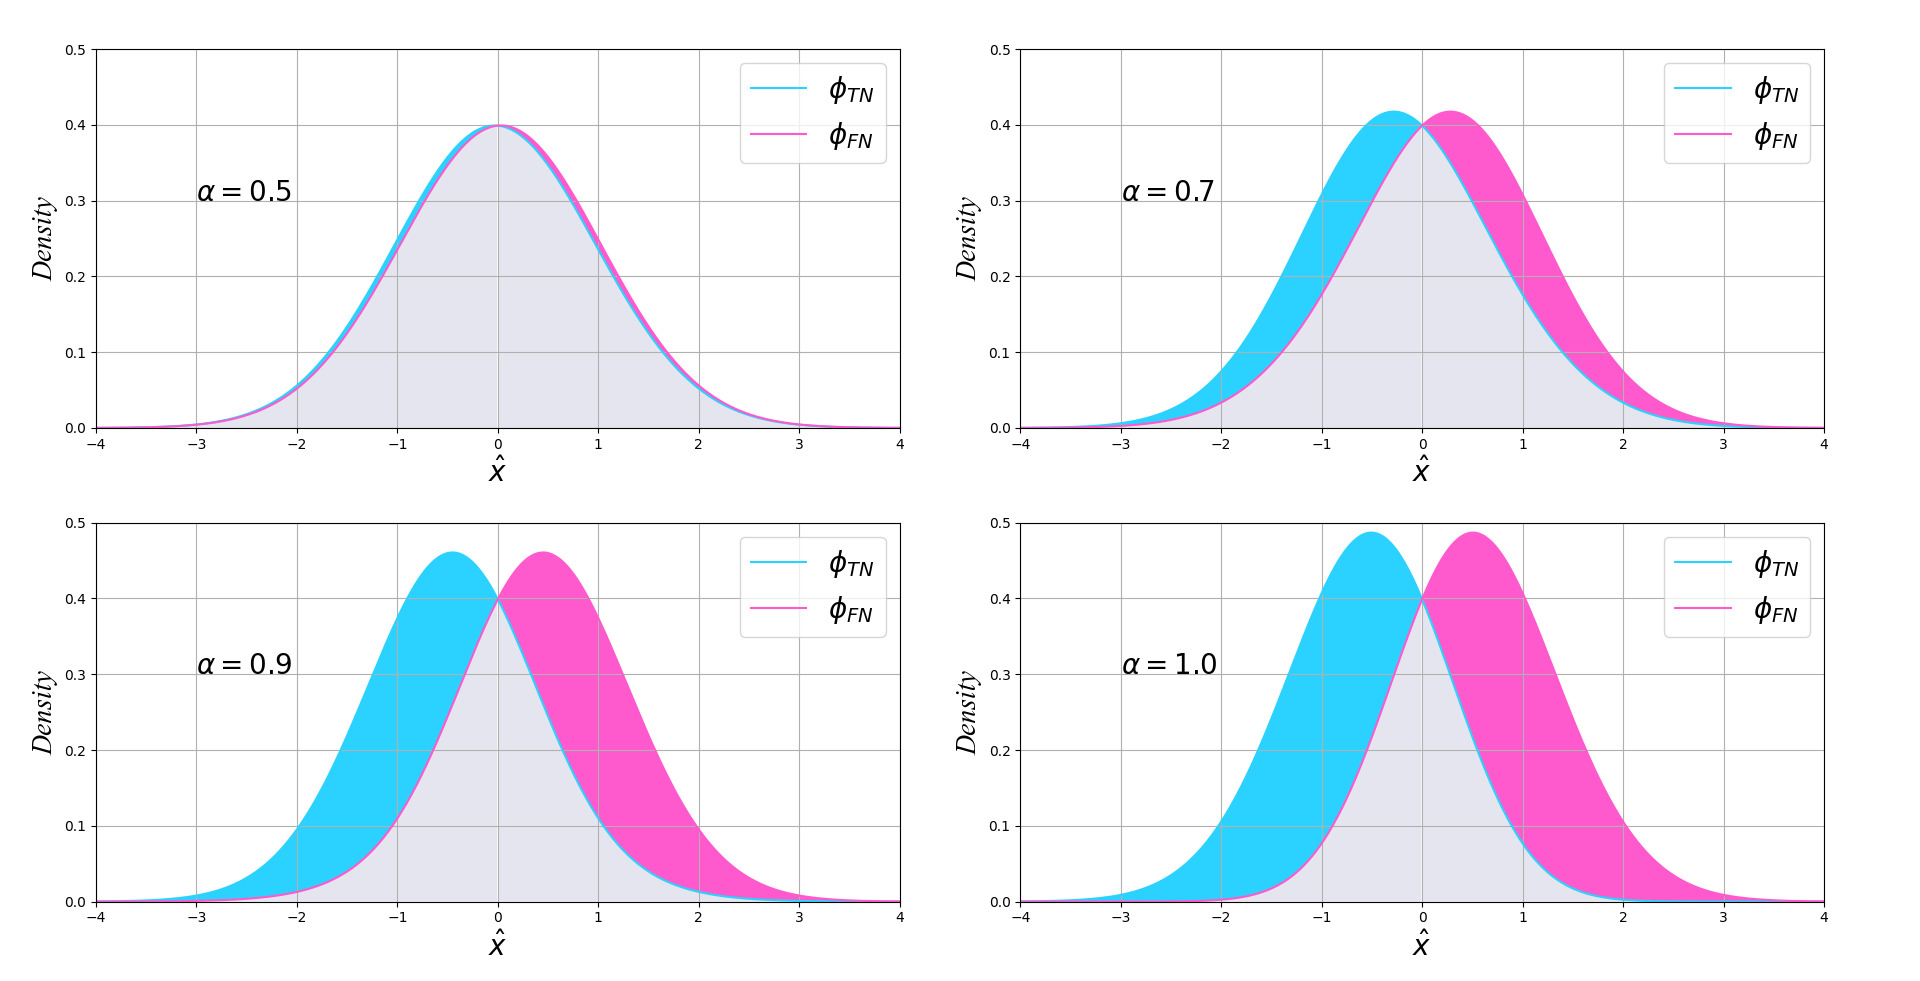
\includegraphics[width=\textwidth]{theorydist.png}
	\caption{不同$\alpha$设定下类条件概率密度示意图}
	\label{Fig:theorydist}
\end{figure}
%*******************************
\begin{eqnarray}
	\small
	\alpha &=& \int\limits_{x \in \mathcal{X}}  \int\limits_{0}^{+\infty} \int\limits_{0}^{+\infty} \mathbb I (\hat{x}^+ \ge \hat{x}^-)  p(\hat{x}^+ , \hat{x}^-) p(x) d\hat{x}^+  d\hat{x}^- dx\nonumber\\
	&\simeq& \frac{1}{|\mathcal{D}|} \frac{1}{|\mathcal{D}^+| |\mathcal{D}^-|} \sum_{\mathcal{D}^+}\sum_{\mathcal{D}^-}  \mathbb I (\hat{x}^+ \ge \hat{x}^-) \nonumber \\
	&=& \frac{1}{|\mathcal{D}|} AUC
\end{eqnarray}
因此$\alpha$的值可以通过少部分标记的样本进行经验估计,或者作为超参数。通过在公式~\eqref{eq:order1}和公式~\eqref{eq:order2}中将相似度分数分布$\phi(\hat{x})$设定为$\mathcal{N}(0,1)$,可以作为一个实例,帮助了解$\alpha$如何影响公式~\eqref{eq:phitn}和公式~\eqref{eq:phifn}中的类条件概率密度$\phi_{\textsc{Tn}}(\hat{x})$和$\phi_{\textsc{Fn}}(\hat{x})$,如图~\ref{Fig:theorydist}所示。较大的$\alpha$值导致$\phi_{\textsc{Tn}}(\hat{x})$与$\phi_{\textsc{Fn}}(\hat{x})$之间的区分度更高,因为更好的编码器会将具有不同类标签的样本编码得更正交~\cite{Chuang:2020:NIPS}。需要说明的是,将布$\phi(\hat{x})$设定为$\mathcal{N}(0,1)$只是为了解释说明,后续计算不涉及任何对$\phi(\hat{x})$的具体形态的假设。

真负例分数的类条件概率密度$\phi_{\textsc{Tn}}(\hat{x})$,就是理想的\textit{目标抽样群体},描述了来自真负样本群体的相似度分数分布,来自这部分的样本计算得到的损失函数,即为有监督损失。需要关注的是~\ref{Fig:illustrative}中$x_1^\prime$(狼)这个困难负样本示例。它是与锚点类别不同的负样本,但是由于和锚点很相似,难以区分,这种情况对应于图\ref{Fig:openball}(b)中所描述的情况,即真负例距离锚点更近,属于被错分的样本。这类硬负例的相似度分数密度对应于式\eqref{eq:phitn}中的第二项,即$(1-\alpha)\phi_{(2)}(\hat{x})$,称为\textit{困难负样本成分};另外一类容易负样本如\ref{Fig:illustrative}中$x_5^\prime$(猫),它容易区分,对应于图\ref{Fig:openball}(a)中所描述的情况,这类容易负样本的相似度分数密度对应于式\eqref{eq:phitn}中的第一项,称为\textit{容易负样本成分}。

困难负样本由于与锚点非常相似,难以区分,总是被编码到锚点比较近的距离,不利于下游分类任务。为了加大对真负例总体$\phi_{\textsc{Tn}}(\hat{x})$中困难负样本成分$(1-\alpha)\phi_{(2)}(\hat{x})$的惩罚力度,引入一个参数$\beta \in [0.5, 1]$,对真负例的群体$\phi_{\textsc{Tn}}(\hat{x}) $进行细分,从困难负样本成分中抽样$\beta$的比例,从容易负样本成分中抽样$1-\beta$的比例,构成新的抽样目标:
\begin{eqnarray}
	\phi_{\textsc{Thn}}(\hat{x}) 
	&=& (1-\beta)\alpha  \phi_{(1)}(\hat{x}) +\beta (1-\alpha)  \phi_{(2)}(\hat{x}) \label{eq:tnhard} 
\end{eqnarray}
参数$1-\beta$控制着\textit{易负样本成分}$\alpha \phi_{(1)}(\hat{x})$的比例,而$\beta$控制着被分类器错误分类的\textit{难负样本成分}$(1-\alpha)\phi_{(2)}(\hat{x})$的比例。$\beta= 1$时,新的目标抽样群体$\phi_{\textsc{Thn}}(\hat{x}) $只有困难负样本成分;$\beta = 0.5$时,容易负样本成分和困难负样本的比例与原始抽样目标是一致的;$\beta = 0$时,新的目标抽样群体$\phi_{\textsc{Thn}}(\hat{x}) $只有容易负样本成分;因此,公式~\eqref{eq:tnhard}可以解释为具有困难级别(hardness level)为$\beta$的困难负样本分布,较大的$\beta$值(接近1)导致中包含更高比例的被分类器错误分类的困难负样本成分。

\subsubsection{实际采样群体}
实际采样的样本来自未标注样本,通过正样本和负样本的类条件密度,可以应用全概率公式将边际概率与条件概率联系起来,从而获得未标记数据的密度$\phi_{\textsc{Un}}$
\begin{eqnarray}\label{eq:unlabel}
	\phi_{\textsc{Un}} &=& \tau^-\phi_{\textsc{Tn}} +\tau^+\phi_{\textsc{Fn}}  
\end{eqnarray} 
未标注样本的概率密度决定性因素是伪负例的类先验概率$\tau$。一个伪负例占比为50\%的数据集,和伪负例占比为5\%的数据集,相似度的分数分布差别是很大的。

为了避免混淆,下表梳理了本章出现的密度的符号及含义。
\begin{table*}[h!]\label{table:density}
	\centering
	\caption{概率密度一览表}
	\resizebox{1\textwidth}{!}{
		\begin{tabular}{cllc}
			\toprule[1.2pt]	
			\textbf{符号}&\textbf{含义}& \textbf{描述}&是否包含参数化假设 \\ \hline		
			$\phi(\hat{x})$ & 特定于锚点的相似度分数分布 & 由锚点$x$,相似度函数,以及编码器结构$f$决定 & 否 \\
			$\phi_{(1)}(\hat{x})$ &次序统计量$X_{(1)}$的分布& 由$\phi(\hat{x})$决定& 否\\
			$\phi_{(2)}(\hat{x})$ &次序统计量$X_{(2)}$的分布& 由$\phi(\hat{x})$决定 & 否 \\\hline
			$\phi_{\textsc{Tn}}(\hat{x})$&真负例相似度分数的类条件概率密度& \textbf{目标抽样群体} & 否 \\
			$\phi_{\textsc{Fn}}(\hat{x})$&伪负例相似度分数的类条件概率密度& -- & 否 \\
			$\phi_\textsc{Thn}(\hat{x})$& 硬负例的相似度分数分布&通过细分$\phi_{\textsc{Tn}}(\hat{x})$得到的\textbf{新的目标抽样群体}& 否  \\\hline
			$\phi_{\textsc{Un}}(\hat{x})$& 未标记样本的相似度分数分布&\textbf{实际抽样群体}& 否  \\
			\hline
			\bottomrule[1.2pt]
			
			~		\end{tabular}
	}
\end{table*}

需要特别强调的是相似度分数分布$\phi(\hat{x})$与未标记样本的相似度分数分布$\phi_{\textsc{Un}}(\hat{x})$的区别:前者由锚点$x$,相似度函数,以及编码器结构$f$决定,包含了所有的可能的类先验$\tau$可能的取值的分布;而后者未标记样本的相似度分数分布$\phi_{\textsc{Un}}(\hat{x})$由特定的类先验$\tau$决定。

\subsubsection{蒙特卡洛重要性采样}
上面的分析只得到了目标抽样群体和实际抽样群体密度函数的抽象表达式,但是足以计算重要性权重$\omega_i$。根据经典的蒙特卡洛重要性采样~\cite{Hesterberg:1988,Bengio:2008:TNN}的计算步骤,重要性权重的计算公式为目标抽样群体与实际抽样群体的密度比
%\begin{eqnarray}
%	\mathbb E_{\hat{x} \sim \psi}  \hat x 	&=& \int_{+\infty}^{+\infty} \hat x  \frac{\phi_\textsc{Thn}(\hat{x};\alpha, \beta)}{\phi_{\textsc{Un}}(\hat{x})} \phi_{\textsc{Un}}(\hat{x}) d\hat{x} \nonumber \\
%	&=&   \mathbb E_{\hat{x} \sim \phi_{\textsc{Un}}} \hat x  \frac{\phi_\textsc{Thn}(\hat{x};\alpha, \beta)}{\phi_{\textsc{Un}}(\hat{x})} \nonumber\\
%	&\simeq&\frac{1}{N}  \sum_{i=1}^{N} \omega_i \hat{x}_i  \label{eq:impor}
%\end{eqnarray}
\begin{eqnarray}
	\omega_i(\hat x_i;\alpha, \beta)&=& \frac{\phi_\textsc{Thn}(\hat{x};\alpha, \beta)/Z}{\phi_{\textsc{Un}}(\hat{x})} \label{eq:ome} \\
	&=& \frac{1}{Z} \frac{(1-\beta)\alpha + (\beta-\alpha)\Phi(\hat{x})}{\alpha\tau^- + (1- \alpha)\tau^+  + (1-2\alpha)\Phi(\hat{x})(\tau^- -\tau^+)}  \label{eq:ome1}
\end{eqnarray}
其中Z为目标抽样分布$\phi_\textsc{Thn}$的归一化配分因子,可以通过边际积分准确计算如下:
\begin{eqnarray}
	Z &=& \int_{ - \infty } ^{\infty} \phi_{\textsc{Thn}}(\hat{x})  d \hat{x} \nonumber \\
	&=& \int_{-\infty}^{\infty}  [(1-\beta)\alpha  \phi_{(1)}(\hat{x}) +\beta (1-\alpha)  \phi_{(2)}(\hat{x})]  d \hat{x} \nonumber \\
	&=& (1-\beta)\alpha + \beta (1-\alpha)
\end{eqnarray}

可以看到式\eqref{eq:ome1}中的重要性权重$\omega_i(\hat x_i;\alpha, \beta)$是累积分布函数(CDF)$\Phi (\hat{x})$的函数, 其中密度函数$\phi{(\hat{x})}$由于式\eqref{eq:ome1}的分式形式,可以通过约分被消去,进而无需对密度函数的具体形式做出参数化假设。只需要
$\Phi (\hat{x})$的值,就可以计算相应的重要性权重。

下面介绍如何计算累积分布函数(CDF)$\Phi (\hat{x})$。
%\begin{eqnarray}
%	\phi_{\textsc{Un}}(\hat{x}) &=& \tau^-\phi_{\textsc{Tn}}(\hat{x}) +\tau^+\phi_{\textsc{Fn}}(\hat{x}) \nonumber \\
%	&=& 2\phi(\hat{x})[\alpha\tau^- + (1- \alpha)\tau^+  + (1-2\alpha)\Phi(\hat{x})(\tau^- -\tau^+)] \label{eq:unlabel1}
%\end{eqnarray}
对公式\eqref{eq:unlabel}等号两侧进行积分,可得:
\begin{eqnarray}
\int_{-\infty}^{\hat x}  \phi_{\textsc{Un}}(t) dt 
	&=& \int_{-\infty}^{\hat x} \tau^-\phi_{\textsc{Tn}}(t) +\tau^+\phi_{\textsc{Fn}}(t) dt \label{eq:un}\\
	&=& \int_{-\infty}^{\hat x} 2\phi(t)[\alpha\tau^- + (1- \alpha)\tau^+  + (1-2\alpha)\Phi(t)(\tau^- -\tau^+)] dt\nonumber\\ 
	&=&  2[\alpha\tau^- + (1- \alpha)\tau^+]\int_{-\infty}^{\hat x} \phi(t) dt + (1-2\alpha)(\tau^- -\tau^+)\int_{-\infty}^{\hat x} 2 \phi(t) \Phi(t) dt \nonumber\\
	&=& 2[\alpha\tau^- + (1- \alpha)\tau^+] \Phi(\hat{x}) + (1-2\alpha)(\tau^- -\tau^+)\Phi^2(\hat{x}) \label{eq:unlabel33}
\end{eqnarray}
式\eqref{eq:un}等号左侧对密度函数积分,正是累积分布函数$\Phi_{\textsc{Un}}(\hat{x})$。记
\begin{eqnarray}
	a &=&  (1-2\alpha)(\tau^- -\tau^+)\nonumber \\
	b &=& 2[\alpha\tau^- + (1- \alpha)\tau^+] \nonumber
\end{eqnarray}
那么式\eqref{eq:unlabel33}可以简化为一个一元二次方程
\[\Phi_{\textsc{Un}}(\hat{x})= a\Phi^2(\hat{x}) + b\Phi(\hat{x})\]
根据求根公式有
\begin{eqnarray}\label{eq:Phi}
	\Phi(\hat{x}) = \frac{-b+\sqrt{b^2+4a\Phi_{\textsc{Un}}(\hat{x})}}{2a}
\end{eqnarray}
另外一个解$\Phi(\hat{x}) = \frac{-b-\sqrt{b^2+4a\Phi_{\textsc{Un}}(\hat{x})}}{2a}$ 小于0舍去,因为它不在累积分布函数的取值区间内。上式建立了两个累积分布函数之间的关系,只要给出未标注样本的累积分布函数$\Phi_{\textsc{Un}}(\hat{x})$,就可以计算得到所需的$\Phi(\hat{x})$,从而用于计算重要性权重。
%%*******************************Fig~\ref{fig:cdf_trans} illustrates the transformation of two cumulative distribution functions $\Phi(\hat{x})$ and $\Phi_{\textsc{Un}}(\hat{x})$, where we fixed $\tau^+=0.1$. 
%\begin{figure*}[h!]
%	\centering
%	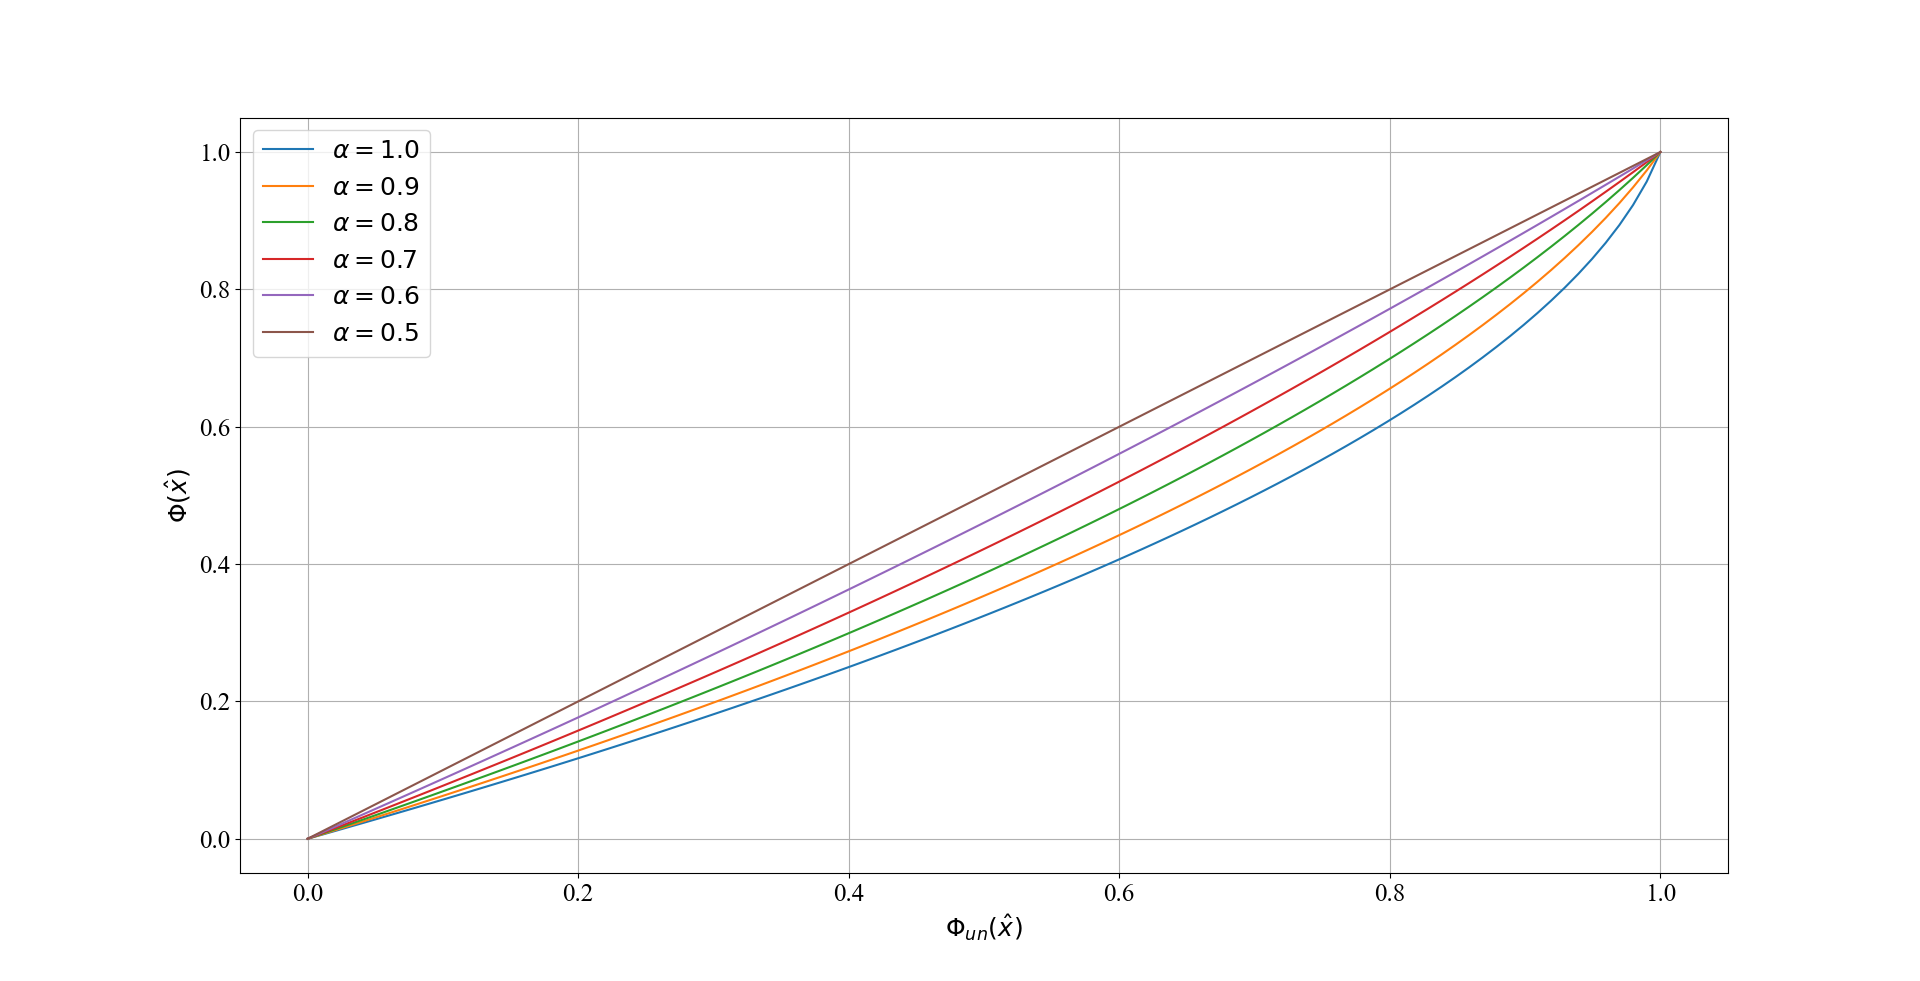
\includegraphics[width=\textwidth]{cdf_trans.png}
%	\caption{The transformation of two cumulative distribution functions $\Phi(\hat{x})$ and $\Phi_{\textsc{Un}}(\hat{x})$, where x-axis is the  C.D.F of unlabeled samples $\hat{\Phi}_{\textsc{Un}}$ , and y-axis is the anchor specific C.D.F $\Phi(\hat{x})$. From Eq~\eqref{eq:unlabel1}, it can be seen that when $\alpha=0.5$, which means the encoder makes random guesses, or when $\tau^+=0.5$, which means the prior class probabilities of positive and negative examples are equal, $\Phi(\hat{x})=\Phi_{\textsc{Un}}(\hat{x})$.}
%	\label{fig:cdf_trans}
%\end{figure*}
%%*******************************

最后只剩下如何计算未标注样本的累积分布函数$\Phi_{\textsc{Un}}(\hat{x})$。可以使用如下经验分布函数进行近似:
\begin{equation}\label{eq:puedf}
	\hat \Phi_{\textsc{Un}} (\hat{x}) = \frac{1}{N} \sum_{i=1}^{N}\mathbb{I}_{|X_i \leq \hat{x}|},
\end{equation}
根据根据Glivenko定理~\cite{glivenko:1933}所述,经验累积分布函数$\hat{\Phi}_{\textsc{Un}}(\hat{x})$收敛于标准的累积分布函数(C.D.F) $\Phi_{\textsc{Un}}(\hat{x}) = \int_{-\infty}^{\hat{x}} \phi_{\textsc{Un}}(t)dt$。

%通过使用宏$AUC$度量对编码器进行表征,引入可计算的经验累积分布函数作为似然度量来构建后验估计器,

到目前为止,重要性权重的计算已经介绍完毕。它们的计算只涉及以下内容:(i) $\hat{\Phi}_{\textsc{Un}} (\hat{x}) \in [0,1]$,它代表了贝叶斯视角下的\textit{样本信息},可以直接从N个未标注样本计算得出。它包含了当前模型对未标注样本是伪负例$\hat x \in \textsc{Fn}$的概率解释:对于较大的$\hat{x}$值(与锚点的嵌入距离更接近),$\hat{\Phi}_{\textsc{Un}} (\hat{x})$输出一个更接近于1的值,表明$\hat{x}$是一个来自伪负例的相似度观测值。换言之,$\hat{\Phi}_{\textsc{Un}} (\hat{x})$反映了当前模型对未标注样本的分类结果。(ii)类别先验概率$\tau$。由样本信息和先验信息计算到的权重$\omega_i$自然包含后验信息,因此把经过上述重要性权重加权的自监督对比损失成为贝叶斯自监督对比损失(Bayesian self-supervised contrastive loss, BCL)。定理~\ref{the:poster}分析了权重$\omega$与样本未真负例的后验概率之间的联系,它们是严格的线性关系。


参数$\alpha\in [0.5,1]$对应于编码器的宏AUC度量,控制着样本信息的置信水平。在训练过程中,可以通过验证数据集进行经验估计。参数$\beta\in [0.5,1]$对应于真负例群体中被错误分类的\textit{困难负样本成分}的比例,是一个根据任务场景所需的硬负例挖掘困难等级(hardness level)决定的超参数。在计算对比损失时,还是使用从数据分布中采样的未标记样本$x_i^\prime$,但使用相应的重要性权重$\omega(\hat{x},\alpha, \beta)$进行加权,以校正目标采样群体和实际采样群体之间的偏差。那么,给定N个随机负采样的未标注样本$\{x_i^\prime\}_{i=1}^N$,校正后的损失函数形式为
\begin{eqnarray}\label{eq:bcl}
	\mathcal{L}_\textsc{~Bcl}=  \mathbb E_{\substack{x \sim p_d\\~x^+ \sim p^+\\\color{blue}{~x^\prime \sim p_d}}} [-\log \frac{e^{f(x)^Tf(x^+)}}{e^{f(x)^Tf(x^+)} +  \sum_{i=1}^N  \omega_i \cdot e^{f(x)^Tf(x^\prime_i)} }]
\end{eqnarray}

\section{算法实现与时间复杂度分析}
\subsection{算法步骤}
重要性权重计算的逻辑有一些复杂,主要是解析目标采样分布和实际采样分布的抽象函数表达式,但计算步骤是很简单的,相对于标准的对比损失函数,只涉及三个额外计算步骤,如下伪代码所示。
\begin{algorithm}[!]
	\small
	\caption{贝叶斯自监督对比学习算法(BCL)伪代码}\label{5-Alg:1}
	\KwIn{数据条目组织形式为(锚点$x$,正例$x^+$,N个随机负采样的未标注样本$x_1^\prime, \cdots x_n^\prime$)的训练集$\mathcal{D}$,正例类先验$\tau^+$,去偏超参数$\alpha$, 硬负例难度超参数$\beta$。}
	\KwOut{模型参数$\Theta \in \mathbb{R}^d$}
	~~计算正例分数$\hat{x}^+ = e^{f(x)^Tf(x^+)}$;\\
	计算N个未标注样本分数$\hat{x}_i = e^{f(x)^Tf(x^\prime_i)}$, $i = 1,2,\cdots, N$ ;\\
	\For{$i = 1,2,\cdots, N$}{
		~~通过公式\eqref{eq:puedf}计算经验分布函数$\hat \Phi_{\textsc{Un}} (\hat{x}_i)$; \\
		通过公式\eqref{eq:Phi}计算分布函数$\Phi(\hat{x}_i)$;\\
		通过公式\eqref{eq:ome1}计算重要性权重$\omega_i$;\\
		计算损失函数$\mathcal{L} = -\log \frac{\hat{x}^+}{\hat{x}^+ + \sum_{i=1}^N \omega_i \cdot \hat{x}_i}$;\\
		根据$\mathcal{L}$相对于$\Theta$的梯度更新参数$\Theta$;
	}
	\KwResult{模型参数$\Theta$。}
\end{algorithm}

将数据条目组织为(锚点$x$,正例$x^+$,N个随机负采样的未标注样本$x_1^\prime, \cdots x_n^\prime$)的元组结构,可以通过重写Pytorch的\verb|get_item|方法或\verb|collate_fn|方法实现,二者类似。第\ref{cha:fourthsection}章的算法\ref{4Alg2:1}提供了重写\verb|collate_fn|方法的算法伪代码,本章不再赘述。

\subsection{时间复杂度分析}
本章所介绍的方法,是上一章从$N=1$个负例向多个负例的更一般的对比损失的推广,但基本思想都是估计校正,不涉及显式的负采样,仍然使用in-batch内的随机负样本计算对比损失,因此也不涉及对mini-batch以外的额外计算和存储开销。由于要计算重要性权重,从而对对比损失进行校正,从而引入了额外的时间复杂度。下面以标准的InfoNCE损失为基准,分析本章所提出的方法的计算的额外开销。

在计算标准的InfoNCE损失时,也需要正向计算正例的相似度分数以及未标注样本的相似度分数,然后反向传播按照梯度下降算法更新参数,那么InfoNCE也要执行算法\ref{5-Alg:1}的\verb|for|循环内的最后两行。因此贝叶斯自监督对比学习的额外计算开销主要是:(1)通过公式\eqref{eq:puedf}计算经验分布函数$\hat \Phi_{\textsc{Un}} (\hat{x}_i)$,时间复杂度为$\mathcal{O}(N)$;(2)通过公式\eqref{eq:Phi}计算分布函数$\Phi(\hat{x}_i)$,时间复杂度为$\mathcal{O}(1)$;(3)通过公式\eqref{eq:ome1}计算重要性权重$\omega_i$,时间复杂度为$\mathcal{O}(1)$。计算重要性权重的公式\eqref{eq:ome1}尽管看起来很复杂,但是都是标量计算,因此是常数时间复杂度。因此,一个样本的重要性权重$\omega_i$额外计算开销为$\mathcal{O}(N)$,通常远低于编码样本$f(x)$的时间复杂度,是可以忽略的。在本章实验部分对比了实际的运行时间,本方法和基准方法InfoNCE相比,有着几乎相同的实际运行时间。

\section{贝叶斯自监督对比损失的理论分析}
本章的\ref{subsec:fh}小节分析了,基于对比学习“正例对齐、负例均匀”的任务考量,合意的权重$\omega_i$与相应的未标注样本$x^\prime_i$的所属类别相联系:未标注样本$x^\prime_i$是真负例的概率越低,权重$\omega_i$值应该越小(伪负例去偏要求);未标注样本$x^\prime_i$是真负例的概率越高,权重$\omega_i$应该越大(硬负例挖掘要求)。那么,本章的$\omega_i$值是否满足上述要求?本章计算的$\omega_i$与样本是真负例的概率有什么联系?此外,经过对随机样本的重要性加权以后计算得到的贝叶斯自监督对比损失,与完全监督数据计算得到的对比损失有什么联系?
%*******************************
\begin{figure}[!]
	\centering
	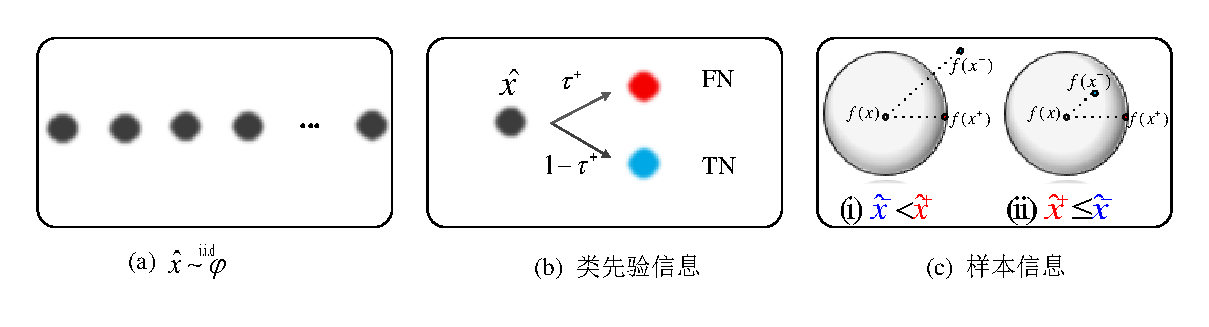
\includegraphics[width=\textwidth]{PCU.pdf}
	\caption{抽象数学模型示意图}
	\label{Fig:formulation}
\end{figure}
%*******************************

为了回答上面的问题,首先考虑一个如图\ref{Fig:formulation}描述的抽象数学模型:图\ref{Fig:formulation}(a)表示未标注样本$x^\prime_i$与锚点的相似度观测值$\hat{x}$为随机变量,假设它独立同分布于某个未知分布$\phi$,图\ref{Fig:formulation}(b)表示未标注样本观测值中,来自正类的占比为$\tau^+$,相应的观测值记为$\hat{x}^+$;未标注样本观测值中,来自负类的占比为$\tau^- = 1-\tau^+$,相应的观测值记为$\hat{x}^-$。图\ref{Fig:formulation}(c)表示正例的观测值以$\alpha$的概率小于负例的观测值。

图\ref{Fig:formulation}(a)是一个并不严格的假设,因为并没有对未知分布$\phi$的具体形态做出规定。对于不同的锚点,锚点与未标记样本的相似度分数观测值的分布$\phi$可以不同;图\ref{Fig:formulation}(b)不是假设,而是已知条件。正例类先验概率$\tau^+$通常是可以获得的,例如在类别均匀的10分类数据集中,遇到一个与锚点同类(狗)的同类样本的占比,就是1/10。更多面向复杂场景如类别不平衡、PU数据集的类先验$\tau^+$的估计方法可以参考文献\cite{Jain:2016:NIPS,Christoffel:2016:ACML};图\ref{Fig:formulation}(c)也不是假设,而是已知条件。前面的章节讨论了,$\alpha$的含义为当前模型参数下编码器的AUC,可以通过少部分标注样本进行经验估计,或者设定为超参数。

\begin{theorem}[后验概率估计]\label{the:poster}
设$\hat{x}$独立同分布于某未知分布$\phi$。其中,正例$\hat x^+$的占比为$\tau^+$,且$\mathbb P (\hat x^- < \hat x^+)= \alpha$ 。取$\beta = 0.5$,则重要性权重$\omega_i$与样本为真负例的后验概率$P(\textsc{Tn}|\hat{x}_i)$存在如下关系
\[\omega_i = \mathbb P(\textsc{Tn}|\hat{x}_i)/\tau^-\]
\begin{proof}
对于独立同分布于$\phi$的随机变量$\hat{x}$,其次序统计量$X_{(1)}$和$X_{(2)}$的分布为:
\begin{eqnarray}
	\phi_{(1)}(\hat{x}) &=& 2\phi(\hat{x}) [1-\Phi(\hat{x})] \nonumber \\
	\phi_{(2)}(\hat{x}) &=& 2\phi(\hat{x}) \Phi(\hat{x}) \nonumber
\end{eqnarray}
其中$\Phi(\hat{x}) = \int_{ - \infty }^{\hat{x}} \phi(t) dt$ 是概率密度函数$\phi(\hat{x})$对应的累积分布函数。

由于$\mathbb P (\hat x^- < \hat x^+)= \alpha$,则
\[\mathbb P (\hat x^- \geq \hat x^+)=1- \alpha\]

那么$\hat{x}$中的负例类别$\hat x^-$的概率密度是次序统计量$X_{(1)}$和$X_{(2)}$的概率密度以系数$\alpha$进行混合
\begin{eqnarray}
	\phi_{\textsc{Tn}}(\hat{x}) = \alpha \phi_{(1)}(\hat{x}) + (1-\alpha)\phi_{(2)}(\hat{x}) \nonumber
\end{eqnarray}
其中,负例类别$\hat x^-$的概率密度,也称类条件概率密度。类似地,正例类别$\hat x^+$的类条件概率密度为
\begin{eqnarray}
	\phi_{\textsc{Fn}}(\hat{x}) = \alpha \phi_{(2)}(\hat{x}) + (1-\alpha)\phi_{(1)}(\hat{x})\nonumber
\end{eqnarray}
那么,观测到的未标注样本的概率密度为
\begin{eqnarray}
	\phi_{\textsc{Un}}(\hat{x}) &=& \tau^-\phi_{\textsc{Tn}}(\hat{x}) +\tau^+\phi_{\textsc{Fn}}(\hat{x}) \nonumber 
\end{eqnarray} 
其中$\tau^- = 1- \tau^+$代表负类的占比。以上是本章方法部分已有结论,不再详细论述。那么式\eqref{eq:ome}给出的$\omega_i(\hat{x}_i;\alpha,\beta=0.5)$可以计算为
\begin{eqnarray}
	\omega_i&=& \frac{\phi_\textsc{Thn}(\hat{x};\alpha, \beta=0.5)/Z}{\phi_{\textsc{Un}}(\hat{x})}  \nonumber \\
 &=&\frac{ (1-0.5)\alpha  \phi_{(1)}(\hat{x}) +0.5 (1-\alpha)  \phi_{(2)}(\hat{x}) }{(1-0.5)\alpha + 0.5 (1-\alpha)} \cdot \frac{1}{\phi_{\textsc{Un}}(\hat{x})}\nonumber\\
	&=& [\alpha\phi_{(1)}(\hat{x})+(1-\alpha)  \phi_{(2)}(\hat{x})] \cdot  \frac{1}{\phi_{\textsc{Un}}(\hat{x})} \nonumber\\
	&=& \phi_\textsc{Tn}(\hat{x})/ \phi_{\textsc{Un}}(\hat{x})\label{eq:ratio}
\end{eqnarray}
上式结论的直观解释是,如果$\beta=0.5$,那么$1-\beta = \beta$,即等比例地从目标抽样群体$\phi_{\textsc{Tn}}(\hat{x})$中选取\textit{容易负样本成分}$\alpha  \phi_{(1)}(\hat{x})$和\textit{困难负样本成分}$(1-\alpha)  \phi_{(2)}(\hat{x})$,那么新的目标抽样群体$\phi_\textsc{Thn}(\hat{x};\alpha, \beta=0.5)/Z$的概率密度与真负例的类条件概率密度$\phi_\textsc{Tn}(\hat{x})$相等,从而重要性权重为真负例类条件概率密度$\phi_\textsc{Tn}(\hat{x})$与未标注样本概率密度$\phi_{\textsc{Un}}(\hat{x})$的比值。

对式\ref{eq:ratio}的结果进行简单的代数变换,有
\begin{eqnarray}
\omega_i &=& \frac{\phi_\textsc{Tn}(\hat{x})\cdot \tau^-}{\phi_\textsc{Un}(\hat{x})} \cdot \frac{1}{\tau^-} \label{eq:oper1}\\
&=&\frac{\phi_\textsc{Tn}(\hat{x}) \tau^-}{\tau^-\phi_{\textsc{Tn}}(\hat{x})  +\tau^+\phi_{\textsc{Fn}}(\hat{x})} \cdot \frac{1}{\tau^-}\label{eq:oper2}\\
&=& p(\textsc{Tn}|\hat{x}_i) \frac{1}{\tau^-} \label{eq:oper3}
\end{eqnarray}
式\eqref{eq:oper1}是先乘以负例的类先验$\tau^-$,然后再除以负例的类先验。式\eqref{eq:oper2}中,第一项分子类条件概率密度$\phi_\textsc{Tn}(\hat{x})$的含义是真负例类的条件概率密度$p(\hat{x}|\textsc{Tn})$,乘以负例的类先验$\tau^-$,得到联合概率分布$p(\hat{x},\textsc{Tn})$。同样地,分母的含义为$p(\hat{x},\textsc{Tn})+p(\hat{x},\textsc{Fn})=p(\hat{x})$。因此,式\eqref{eq:oper3}正是贝叶斯公式的结果。证毕。
\end{proof}
\end{theorem}
定理\ref{the:poster}的结果表明,本方法计算得到的重要性权重与样本为真负例的后验概率之间的严格线性关系。一个未标注样本是真负例的后验概率越低,计算得到的权重$\omega_i$越小,满足伪负例去偏原则;一个未标注样本是真负例的后验概率越低,计算得到的权重$\omega_i$越大,满足硬负例挖掘原则。因此,本方法计算得到的重要性权重本章\ref{subsec:fh}小节所分析的合意的重要性权重的要求。这也是本方法与现有的基于重要性加权的方法HCL~\cite{Robinson:2021:ICLR}的主要区别,HCL的权重只和未标注样本相似度分数$\hat{x}^\beta$相联系,相似度分数越高的样本分配的权重越大。


\begin{theorem}[渐进一致估计]
设$\hat{x}$独立同分布于某未知分布$\phi$。其中,正例$\hat x^+$的占比为$\tau^+$,且$\mathbb P (\hat x^- < \hat x^+)= \alpha$ 。取$\beta = 0.5$,当负例个数$N\rightarrow \infty$时,有
\[ \mathcal{L}_\textsc{~Bcl}\rightarrow\mathcal{L}_\textsc{~Sup} \]

\begin{proof}
主要思路是通过勒贝格支配收敛定理对极限运算和积分运算交换运算次序,然后使用重要采样的性质进行代数变换。
\begin{eqnarray}
	\lim_{N\rightarrow \infty} \mathcal{L}_\textsc{~Bcl} &=& \lim_{N\rightarrow \infty}   \mathbb E_{\substack{x \sim p_d\\~x^+ \sim p^+\\~x^\prime \sim p_d}} -\log[ \frac{e^{f(x)^Tf(x^+)}}{e^{f(x)^Tf(x^+)} +  \sum_{i=1}^N  \omega_i\cdot e^{f(x)^Tf(x^\prime_i)} }]  \label{eq:lebes1}\\ 
	&=&   \mathbb E_{\substack{x \sim p_d\\~x^+ \sim p^+\\~x^\prime \sim p_d}} \lim_{N\rightarrow \infty} -\log[ \frac{e^{f(x)^Tf(x^+)}}{e^{f(x)^Tf(x^+)} +  \sum_{i=1}^N  \omega_i\cdot e^{f(x)^Tf(x^\prime_i)} }]  \label{eq:lebes}\\ 
	&=& \mathbb E_{\substack{x \sim p_d\\~x^+ \sim p^+} }	\lim_{N\rightarrow \infty}[-\log \frac{e^{f(x)^Tf(x^+)}}{e^{f(x)^Tf(x^+)} + N\cdot \mathbb{E}_{\hat{x} \sim \phi_{\textsc{Un}} } \omega\hat x  }] \label{eq:bcldenomitor}
\end{eqnarray}
其中,式\eqref{eq:lebes1}是先对损失函数求期望(即积分运算),然后求极限运算。根据勒贝格控制收敛定理,对于一个有界的可测函数序列$f_n$,有$\lim\limits_{n\rightarrow \infty} \int_{\Omega} f_n =\int_{\Omega} \lim\limits_{n\rightarrow\infty}f_n $。应用该结论,可以交换期望算子和极限算子的运算次序,得到式\eqref{eq:lebes}。

式\eqref{eq:lebes}中,极限运算只作用在分母的第二项中,因为只有分母的第二项包含$N$。由于
\begin{eqnarray}
\lim_{N\rightarrow \infty} \sum_{i=1}^N  \omega_i\cdot e^{f(x)^Tf(x^\prime_i)} &=& \lim_{N\rightarrow \infty} \sum_{i=1}^N  \omega_i\cdot \hat x_i \nonumber \\
&=&  N\mathbb{E}_{\hat{x} \sim \phi_{\textsc{Un}} } \omega \cdot \hat x \nonumber
\end{eqnarray}
于是得到式\eqref{eq:bcldenomitor}。应用式\eqref{eq:ratio}的结论,有
\[\omega(\hat x;\alpha, \beta) = \frac{\phi_\textsc{Tn}(\hat{x})}{\phi_{\textsc{Un}}(\hat{x})}
\]
将上式带入式\eqref{eq:bcldenomitor}分母中的第二项可得
\begin{eqnarray}
	N\mathbb{E}_ {\hat{x} \sim \phi_{\textsc{Un}}} \omega \hat{x} &=& N\int \omega \hat{x}\phi_{\textsc{Un}}(\hat{x}) d\hat{x} \label{eq:imp1}\\
	&=& N\int \hat{x} \frac{\phi_\textsc{Tn}(\hat{x})}{\phi_{\textsc{Un}}(\hat{x})}  \phi_{\textsc{Un}}(\hat{x}) d\hat{x} \label{eq:imp2} \\
	&=& N\int  \hat{x}\phi_\textsc{Tn}(\hat{x})d\hat{x} \nonumber\\
	&=& N \mathbb{E}_ {x^-\sim p^-} e^{f(x)^Tf(x_i^-)}\label{eq:sumtn}\\
	&=& \lim_{N\rightarrow \infty} \sum_{i=1}^Ne^{f(x)^Tf(x_i^-)} \label{eq:imp3}
\end{eqnarray}
式\eqref{eq:imp1}是期望的定义,式\eqref{eq:imp2}是带入重要性权重的结果,式\eqref{eq:sumtn}也是期望的定义。这正是重要性采样的基本性质:使用重要性权重加权来自$\phi_{\textsc{Un}}$总体中的样本,等于目标总体$\phi_{\textsc{Tn}}$的期望。
把式\eqref{eq:imp3}的结果代回式~\eqref{eq:bcldenomitor}中可得
\begin{eqnarray}
	\lim_{N\rightarrow \infty} \mathcal{L}_\textsc{~Bcl} &=&  \mathbb E_{\substack{x \sim p_d\\~x^+ \sim p^+\\~x^- \sim p^-} }	\lim_{N\rightarrow \infty}[-\log \frac{e^{f(x)^Tf(x^+)}}{e^{f(x)^Tf(x^+)} + \sum_{i=1}^Ne^{f(x)^Tf(x_i^-)}}] \nonumber\\
	&=& \lim_{N\rightarrow \infty} \mathbb E_{\substack{x \sim p_d\\~x^+ \sim p^+\\~x^- \sim p^-} }	[-\log \frac{e^{f(x)^Tf(x^+)}}{e^{f(x)^Tf(x^+)} +  \sum_{i=1}^Ne^{f(x)^Tf(x_i^-)} }] \label{eq:dominate}\\
	&=& \lim_{N\rightarrow \infty} \mathcal{L}_\textsc{~Sup}
\end{eqnarray}
式\eqref{eq:dominate}是再次运用勒贝格支配收敛定理交换积分和极限的运算顺序。证毕。
	\end{proof}
\end{theorem}

上述证明过程体现了BCL方法的核心思想:通过重要性加权未标注样本(实际抽样总体)的相似度分数,以近似真负样本(目标抽样总体)的相似度分数的期望值,从而间接地实现对有监督损失的近似。这与第\ref{cha:fourthsection}章通过概率进行近似不同,主要是因为较大的N值导致真实的标签有$2^N$可能,难以枚举。但与第\ref{cha:fourthsection}章的落脚点是一致的,都是获取有监督损失的一致估计。

获得一个与有监督损失一致的估计量,是提升弱监督学习或者无监督学习泛化性能的重要途径。损失函数是模型参数$\Theta$与训练样本$x$的函数$\mathcal{L}(x,\Theta)$,如果给定样本$x$,无监督损失$\mathcal{L}(x,\Theta)$与有监督损失$\mathcal{L}_\textsc{Sup}(x,\Theta)$对于所有可能的模型参数$\Theta$几乎处处(almost everywhere)相等,那么有理由相信,给定相同的训练样本,无监督损失$\mathcal{L}(x,\Theta)$与有监督损失$\mathcal{L}_\textsc{Sup}(x,\Theta)$有相同的极值点$\Theta$,从而在无监督的情况下学到接近于有监督的情况下学到的模型参数,从而取得与有监督学习类似的泛化性能。这是第\ref{cha:fourthsection}章与本章通过估计校正获取一个与有监督损失一致的估计量的意义所在。
%*******************************
\begin{figure}[!]
	\centering
	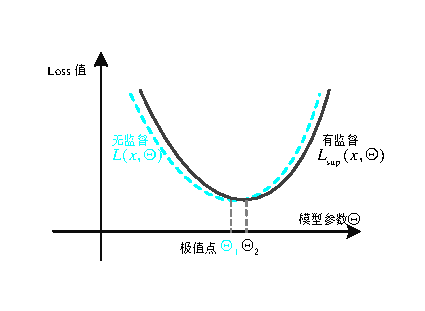
\includegraphics[width=0.8\textwidth]{suploss.pdf}
	\caption{估计校正的的直观阐释示意图}
	\label{Fig:suploss}
\end{figure}
%*******************************

图\ref{Fig:suploss}提供了一个阐释性的例子,固定训练样本$x$,损失值可以看作模型参数$\Theta$的函数。如果,对于所有的模型参数$\Theta$的可能取值,无监督损失函数和有监督损失函数非常接近,那么它们的极值点$\Theta_1$和$\Theta_2$也非常接近,即在无监督数据集中学到接近于有监督数据的模型参数。但需要注意的是,无监督损失和有监督损失的一致性往往以样本数量$N\rightarrow \infty$为前提条件,这是一个理想的情况,在现实中难以实现,有限的样本数量导致估计误差的产生。本章中,在有限样本时,$\mathcal{L}_\textsc{~Bcl}$的估计误差具体体现在三个方面:(1)经验分布函数$\hat{\Phi}_\textsc{Un}(\hat{x})$的估计误差,它是未知的分布函数${\Phi}_\textsc{Un}(\hat{x})$的估计;(2) $\alpha$的估计误差,它是编码器的宏AUC估计;(3)重要性采样的估计误差,它是真负样本的相似度分数期望值的估计。由于涉及因素众多,本章不讨论$\mathcal{L}_\textsc{~Bcl}$估计误差的解析表达式。但是,可以明确的是,较大的N值可以使得上述三个误差都减小,进而$\mathcal{L}_\textsc{~Bcl}$的估计误差会确定性地减小。在数值实验部分也印证了这个结论。此外,较大地N值会推高互信息地下界。因此,在实践中,在GPU显存可承受的范围内,应该选择一个尽可能大的N值。

%%*******************************
%\begin{figure*}[!]
%	\centering
%	\subfloat[Fixed $\alpha$ with different $\beta$ settings.]
%	{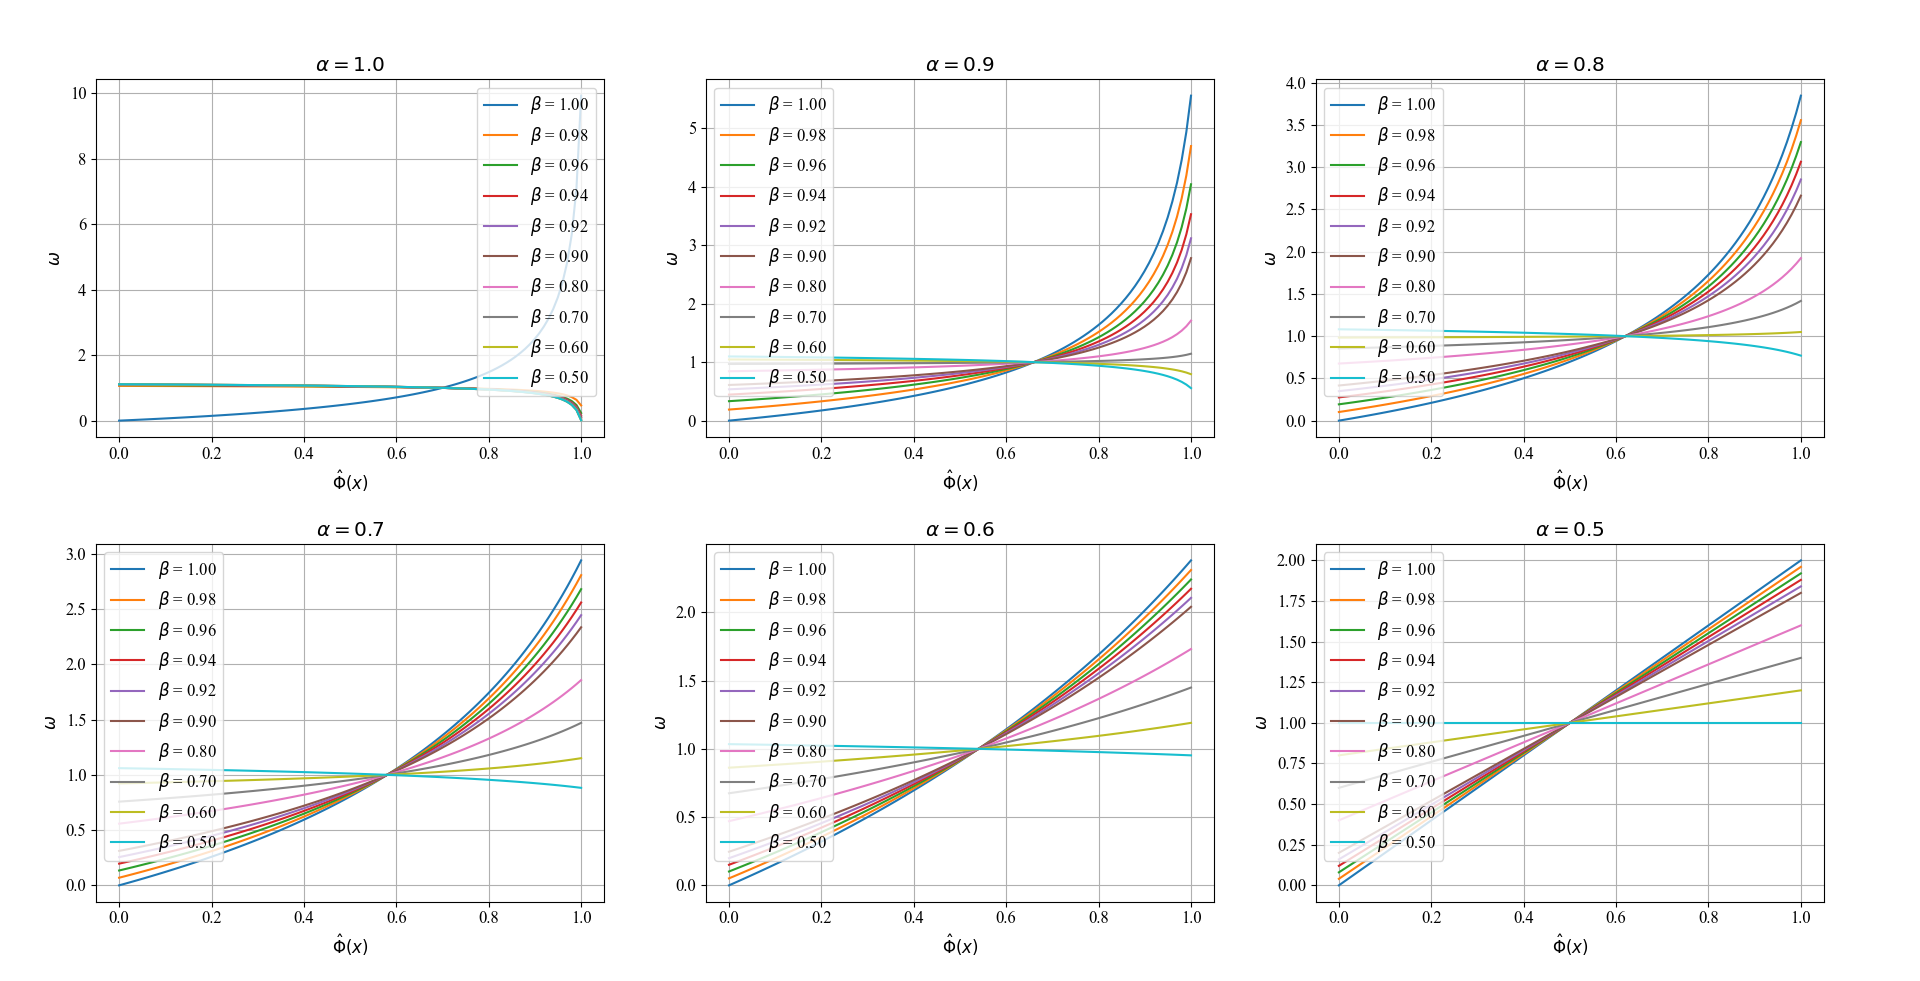
\includegraphics[width=1\textwidth, height=0.5\hsize]{omega_fixalpha.png}\label{fig: omega_a}}\hspace{0.1cm}
%	\subfloat[Fixed $\beta$ with different $\alpha$ settings.]
%	{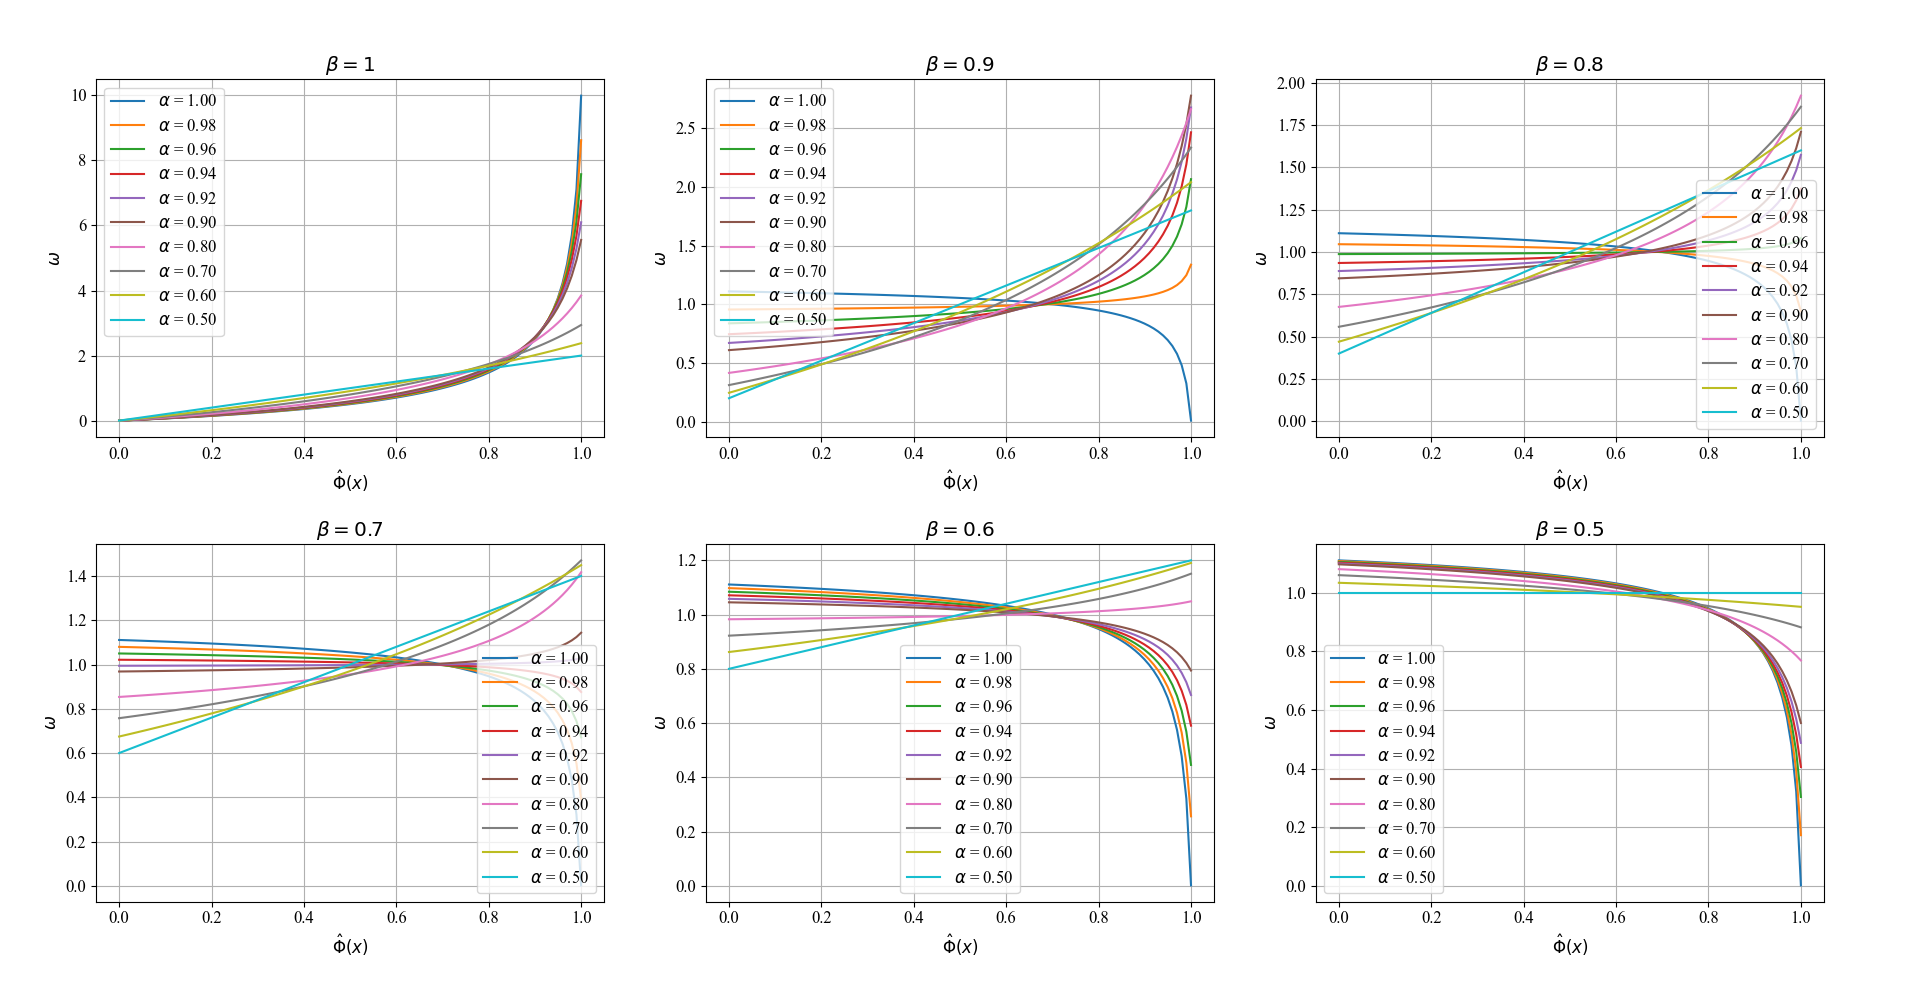
\includegraphics[width=1\textwidth, height=0.5\hsize]{omega_fixbeta.png}\label{fig:omega_b}}
%	\caption{This figure illustrates how the weight $\omega$ changes with respect to $\hat{\Phi}_{\textsc{Un}} (\hat{x})$ under various settings of $\alpha$ and $\beta$, where  $\tau^+$ is fixed at 0.1. X-axis is the empirical C.D.F function $\hat{\Phi}_{\textsc{Un}}$ of unlabeled samples. A value of $\hat{\Phi}_{\textsc{Un}}(\hat{x})=1$ indicates that the instance is the nearest to the anchor, i.e., the highest scored sample. The x-axis can be understood as the hardness level of the samples, with values closer to 1 indicating higher hardness level. The y-axis represents the importance weight $\omega$ calculated based on the BCL computation process. Since $\omega$ is calculated in terms of the empirical C.D.F (relative ranking position) rather than an absolute similarity score, leading it more robust to different temperature scaling settings and encoders. Different values of $\alpha$ and $\beta$ provide flexible options for up-weighting or down-weighting negative samples.}
%	\label{fig:omega}
%\end{figure*}
%%*******************************

\section{实验评估}
由于InfoNCE损失在诸多领域的广泛使用,本章的实验考虑仿真数值实验以及真实数据集实验,在真实数据集上的实验包括个性化推荐任务以及图像分类任务。
\subsection{数值实验}

\subsubsection{实验设置}
前面提到,BCL是通过重要性加权未标注样本(实际抽样总体)的相似度分数$\sum_{i=1}^N \omega_i \cdot \hat{x}_i$,以近似真负样本(目标抽样总体)的相似度分数的期望值,从而间接地实现对有监督损失的近似。那么,对真负样本(目标抽样总体)的相似度分数的期望值估计质量的好坏,决定了是否能够获取与监督损失一致的估计量。在数值实验部分,探讨对真负样本(目标抽样总体)的相似度分数的期望值估计质量的好坏,它决定了与监督损失的一致性,也体现了权重$\omega_i$估计质量的好坏。

前面获得了类条件概率密度(目标抽样群体),以及未标注样本的概率密度(实际抽样群体)的抽象表达式。只要给出任意的相似度分数分布$\phi$,就可以获得类条件概率密度及未标注样本的概率密度的具体表达式。从真负例的类条件概率密度中,可以生成真负例的样本,从而得到期望值;类似地,从伪负例类条件概率密度中,可以生成伪负例样本。二者共同构成了未标注本。按照BCL的计算步骤得到估计值$\sum_{i=1}^N \omega_i \cdot \hat{x}_i$。对比期望值和估计值,可以评估估计质量的好坏。下面介绍样本生成过程。

\subsubsection{样本生成过程}
\textbf{样本生成过程概述:}
为了生成样本,首先随机初始化一个相似度分数分布$\phi$,如均匀分布,高斯分布等。然后就可以生成对应的样本,见图~\ref{fig:generateN}所示,共分为三步:
\par
\textbf{(1)} 以正类先验概率$\tau^+$选择伪负例的标签, 表明一个观测值以$\tau^+$概率来自伪负例$\textsc{Fn}$总体;以负类先验概率$\tau^-=1-\tau^+$选择真负例的标签, 表明一个观测值以$\tau^-$概率来自真负例$\textsc{Tn}$。

\par
\textbf{(2)} 根据所属类别,从类条件概率密度$\phi_{\textsc{Fn}}$ (或 $\phi_{\textsc{Tn}}$)生成随机样本。需要说明的是,即使将$\phi$设置为简单分布,相应的类条件密度$\phi_{\textsc{Fn}}$(或$\phi_{\textsc{Tn}}$)也不再是简单分布。可以使用接受-拒绝采样~\cite{casella2004generalized}技术,只要给出概率密度表达式,就可以生成服从相应分布的样本。具体的技术细节在后面介绍。
%从$\phi_{\textsc{Fn}}$(或$\phi_{\textsc{Tn}}$)中生成样本的细节见算法\ref{Alg:AccRetTN}和算法\ref{Alg:AccRetFN}。
\par
\textbf{(3)} 将生成的样本$\hat{x}$ 映射为 $\exp(\hat{x}/t)$,并混合两个类,作为最终的未标注样本相似度分数观测值。需要说明的是,前面的方法部分没有讨论将观测值$\hat{x}\rightarrow \exp(\hat{x}/t)$的影响,这是因为这是一个严格单调的变换,经过函数映射以后,经验分布函数保持不变:$\Phi_n(\hat{x}) = \Phi_n(\exp(\hat{x}/t))$,因此完全不影响BCL的估计。

重复图~\ref{fig:generateN}描述的过程$N$次,以生成一个锚点的$N$个观测值,并对$M$个锚点重复此过程,就可以得到$M$个锚点所对应的$M$个观测值序列。完整的样本生成过程描述如算法~\ref{Alg:numer}所示。
%*******************************
\begin{figure*}[!]
	\centering
	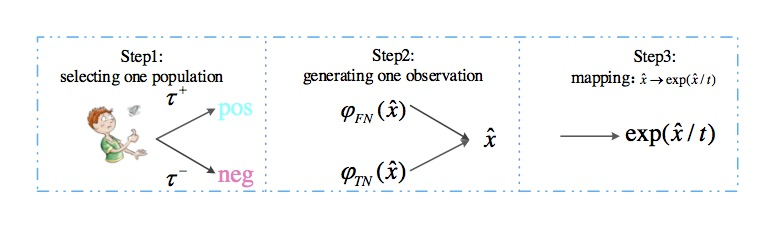
\includegraphics[width=\textwidth]{numerical.jpeg}
	\caption{未标注样本相似度分数生成过程示意图}
	\label{fig:generateN}
\end{figure*}
%*******************************
\begin{algorithm}[!]
	\caption{未标注样本相似度分数观测值生成过程}\label{Alg:numer}
	\KwIn{参数$\alpha$,温度系数$t$,未标注样本数量$N$,锚点个数$M$ }
	\KwOut{未标注样本观测值$\hat{x}$及其对应的标签}
	\BlankLine
	\For{锚点 $m=1, 2, ..., M$}{
		~~$\backslash$$\backslash$ \textit{选定一个任意参数的相似度分数分布$\phi$} \\
		随机选择$[a,b] \subseteq [-1/t^2, 1/t^2]$;\\
		设定$\phi\sim U(a,b) $; \\
		\For{负例 $ j=1, 2, ..., N$}{
			~~$\backslash$$\backslash$ \textit{step1:选择一个总体} \\
			~~$p$ = random.uniform(0,1);\\
			\If{$p \leq \tau^+$}{~~$\backslash$$\backslash$ \textit{step2:从伪负例类条件分布 $\phi_{\textsc{Fn}}$中生成样本} \\
				~~$\hat{x}_j$ = AccRejetSamplingFN($\phi_{\textsc{Fn}}$);\\
				label = False;
			}
			\Else{~~$\backslash$$\backslash$ \textit{step2:从真负例类条件分布$\phi_{\textsc{Tn}}$}中生成样本\\
				~~$\hat{x}_j$ = AccRejetSamplingTN($\phi_{\textsc{Tn}}$); \\
				label = True;
			}
			~~$\backslash$$\backslash$ \textit{step3:函数映射} \\
			$\hat{x}_j = \exp(\hat{x}_j/t)$; \\
			收集$\hat{x}_j$数值及标签;
		}
	}
	\KwResult{未标注样本观测值$\hat{x}$及其对应的标签}
\end{algorithm}

相似度分数分布$\phi$可以是任意的,也称为建议分布(proposal distribution)。对于投影到半径为$1/t$的超球面的表示,相似度观测值的值域为$[-1/t^2, 1/t^2]$。为了方便地控制观测值在其理论最小和最大区间$[-1/t^2,1/t^2]$内,并且先前的研究表明,对比损失在渐近情况下优化了负样本的均匀性~\cite{Wang:2020:ICML},将$\phi$设置为$U(a,b)$以进行数值实验,其中$-1/t^2\leq a \leq b \leq 1/t^2$是针对每个锚点随机选择的。具体而言,原始区间设置为$a=-0.5$,$b=0.5$,并使用$\gamma \in [0,1]$来控制从原始区间的变异程度。$\gamma=1$时,不同锚点之间参数$a,b$参数变异程度最大;$\gamma=0$时,不同的参数$a,b$参数变异程度最小,都为$a=-0.5$,$b=0.5$。

%更规范的$\hat{x}$样本生成过程见如下随机过程描述。
%\begin{definition}[样本函数空间]
%	考虑一个定义在$\mathcal{X} \times \Omega$上的两个变量的函数$X(x,e)$。对于一个锚点$x\in \mathcal{X}$,函数$X(x,e)$是与样本$x_i$相关的随机变量;对于固定的$e\in \Omega$,$X(x,e)$是与锚点相关的样本函数。称${X(x,e): x\in \mathcal{X}, e\in \Omega}$为样本函数空间。
%\end{definition}
%在样本函数空间中,一个锚点$x$确定了分布$\phi$的参数。由于对不同的锚点,$\phi$不要求相同,它模拟了不同锚点可能导致不同观测分布的情况。
%得到了对应于样本函数空间${X(x,e): x\in \mathcal{X}, e\in \Omega}$中的经验观测的集合${\exp(\hat{x}_{mi}/t): m=1,...,M, i=1,\cdots N}$。

\textbf{接受-拒绝采样实现}:生成样本的第二步(图~\ref{fig:generateN}),涉及从从类条件密度$\phi_{\textsc{Tn}}(\hat{x})$生成相应的样本$\hat{x}$,使得$\hat{x} \sim \phi_{\textsc{Tn}}(\hat{x})$。由于类条件概率密度的表达式通常很复杂,不再是简单的均匀分布或者高斯分布,难以直接采样。本节采用标准的接受-拒绝采样方法实现,其基本思想是从建议分布$\phi$中生成样本$\hat{x}$,并以接受概率$p_{\textsc{Tn}}$接受该样本。为了计算接受概率$p_{\textsc{Tn}}$,首先将$\phi_{\textsc{Tn}}(\hat{x})$写为$\phi$的函数
\begin{eqnarray}
	\phi_{\textsc{Tn}}(\hat{x}) &=& \alpha \phi_{(1)}(\hat{x}) + (1-\alpha)\phi_{(2)}(\hat{x}) \nonumber\\
	&=& [2\alpha+(2-4\alpha)\Phi(\hat{x})]\phi(\hat x), \nonumber
\end{eqnarray}
其中$\Phi(\hat{x})$是$\phi(\hat{x})$对应的累积分布函数。接下来,寻找一个最小值$c$满足如下不等式
\[c \cdot \phi(\hat{x}) \geq \phi_{\textsc{Tn}}(\hat{x}),\]
即
\[c \cdot \phi(\hat{x}) \geq  [2\alpha+(2-4\alpha)\Phi(\hat{x})]\phi(\hat x).\]
因此
\begin{eqnarray}
	c &=& min [2\alpha+(2-4\alpha)\Phi(\hat{x})], \Phi(\hat{x}) \in [0,1]\nonumber\\
	&=&2\alpha, \nonumber
\end{eqnarray}
最小值$c$在$\Phi(\hat{x})=0$时取得,由于$2-4\alpha \leq 0$。因此接受概率
\begin{eqnarray}
	p_{\textsc{Tn}} &=& \frac{\phi_{\textsc{Tn}}(\hat{x})}{c \cdot \phi(\hat{x}) } \nonumber \\
	&=& [\alpha + (1-2 \alpha)\cdot \Phi(\hat{x})] /\alpha \nonumber
\end{eqnarray}
从建议分布$\phi(\hat{x})$生成的样本$\hat{x}$以概率$p_{\textsc{Tn}}$被接受,得到了服从分布$ \phi_{\textsc{Tn}}(\hat{x})$的样本,如算法~\ref{Alg:AccRetTN}描述。
\begin{algorithm}[!]
	\caption{~生成服从$\phi_{\textsc{Tn}}$分布的样本的接受拒绝采样算法AccRejetSamplingTN($\phi_{\textsc{Tn}}$)}\label{Alg:AccRetTN}
	\KwIn{参数$\alpha$, 建议分布$\phi$ }
	\KwOut{服从分布$\phi_{\textsc{Tn}}$的样本$\hat{x}$}
	\BlankLine
	~~从分布$\phi$中采样一个随机样本$\hat{x}_j$;\\
	cdf = $\int_{-\infty}^{\hat{x}_j} \phi(t)dt$; \\
	u = random.uniform$(0,1)$; \\
	\While{u $ > [\alpha + (1-2 \alpha)\cdot cdf] /\alpha ~$~ }{
		~~$\backslash$$\backslash$ \textit{样本$\hat{x}_j$被拒绝,重新采样} \\
		从分布$\phi$中采样一个随机样本$\hat{x}_j$;\\
		cdf = $\int_{-\infty}^{\hat{x}_j} \phi(t)dt$; \\
		u = random.uniform$(0,1)$;
	}
	\KwResult{服从分布$\phi_{\textsc{Tn}}$的样本$\hat{x}_j$}
\end{algorithm}

同样地,对于类条件概率密度$\phi_{\textsc{Fn}}$,接受概率的计算步骤类似,为
\[p_{\textsc{Fn}} = [1 - \alpha + (2 \alpha - 1)\cdot \Phi(\hat{x})] / \alpha \]
从建议分布$\phi(\hat{x})$生成的样本$\hat{x}$以概率$p_{\textsc{Fn}}$被接受,得到了服从分布$ \phi_{\textsc{Fn}}(\hat{x})$的样本,如算法~\ref{Alg:AccRetFN}描述。
\begin{algorithm}[!]
	\caption{~生成服从$\phi_{\textsc{Fn}}$分布的样本的接受拒绝采样算法AccRejetSamplingFN($\phi_{\textsc{Fn}}$)}\label{Alg:AccRetFN}
	\KwIn{参数$\alpha$, 建议分布$\phi$}
	\KwOut{服从分布$\phi_{\textsc{Fn}}$的样本$\hat{x}$.}
	\BlankLine
	~~从分布$\phi$中采样一个随机样本$\hat{x}_j$;\\
	cdf = $\int_{-\infty}^{\hat{x}_j} \phi(t)dt$; \\
	u = random.uniform$(0,1)$; \\
	\While{u $ > [1 - \alpha + (2 \alpha - 1)\cdot cdf ] /\alpha ~$~ }{
		~~$\backslash$$\backslash$ \textit{样本$\hat{x}_j$被拒绝,重新采样} \\
		从分布$\phi$中采样一个随机样本$\hat{x}_j$; \\
		cdf = $\int_{-\infty}^{\hat{x}_j} \phi(t)dt$; \\
		u = random.uniform$(0,1)$;
	}
	
	\KwResult{服从分布$\phi_{\textsc{Fn}}$的样本$\hat{x}$}
\end{algorithm}
\begin{figure}[!]
	\centering
	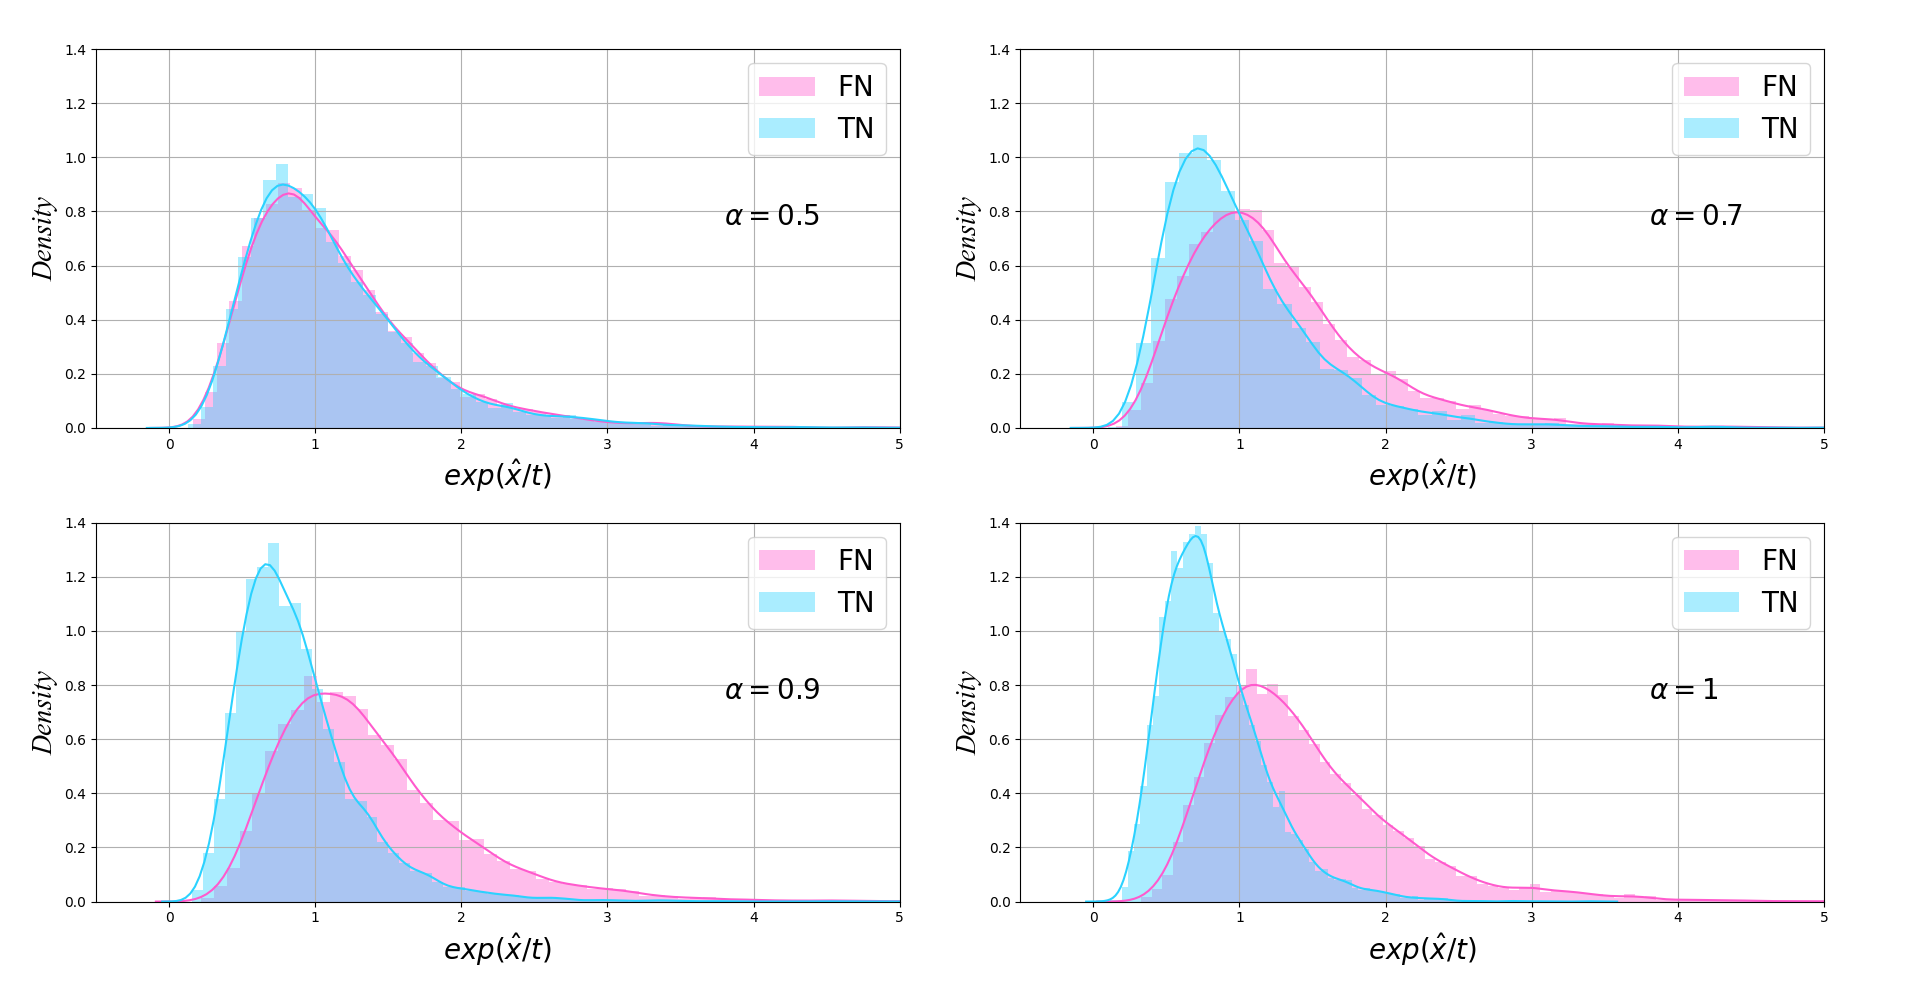
\includegraphics[width=\textwidth]{empiricaldist.png}
	\caption{不同$\alpha$设置下相似度分数的经验分布}
	\label{Fig:empiricaldist}
\end{figure}
\par
根据上述生成过程,图~\ref{Fig:empiricaldist}绘制了生成的样本$\exp(\hat{x}/t)$的经验分布,其中$\phi$设定为标注正态分布,与图~\ref{Fig:theorydist}相对应。其中,$t=2$,$M=1$和$N=20000$。可以看到,图~\ref{Fig:empiricaldist}中的经验分布展现出与使用实际数据集报告的分布~\cite{Robinson:2021:ICLR, Xia:2022:ICML}相似的结构,表明所提出的对样本$\hat{x}$的生成过程描述的有效性。

\subsubsection{对比方法}
在实践中,通常是使用均值作为期望值的经验估计~\cite{Oord:2018:arxiv,Chuang:2020:NIPS,Chen:2020:ICML},因此使用$N$个随机样本中真负例相似度分数的均值作为真值的参考,可以通过如下方式计算
\begin{equation}\label{eq:true}
	\theta_{\textsc{Sup}} = \frac{\sum_{i=1}^N \mathbb{I}(\hat x_i) \cdot \hat{x}_i  }{ \sum_{i=1}^N \mathbb I(\hat{x}_i) },
\end{equation}
其中,$\mathbb{I}(x_i)$是指示函数,如果$\hat{x}_i \in \textsc{Tn}$,则$\mathbb{I}(\hat x_i)=1$;否则,$\mathbb{I}(\hat x_i)=0$,那么式\eqref{eq:true}分子的含义是真负例分数和,分母是真负例的个数,因此式\eqref{eq:true}的含义是真负例分数均值。

对比方法如下:
\begin{eqnarray}
	&&\hat{\theta}_\textsc{Biased} =\frac{1}{N} \sum_{i=1}^{N} \hat{x}_i \label{5Eq:BiasedEstimator} \\
	&&\hat{\theta}_\textsc{Dcl} =  \frac{1}{N\tau^-}  (\sum_{i=1}^{N} \hat{x}_i - N\tau^+ \cdot \frac{\sum_{j=1}^{K} \hat{x}_j^+}{K} ) \label{5Eq:DCLEstimator} \\
	&& \hat\theta_\textsc{Bcl} =\frac{1}{N}  \sum_{i=1}^N \omega_i \cdot \hat{x}_i\label{5Eq:BCLEstimator}
\end{eqnarray}
式~\eqref{5Eq:BiasedEstimator}是标准的InfoNCE损失\cite{Oord:2018:arxiv}对应的估计量,含义为未标注样本的相似度分数均值。式\eqref{5Eq:DCLEstimator}是DCL\cite{Chuang:2020:NIPS}方法所对应的估计量,其含义在第\ref{cha:fourthsection}章的实验部分介绍了,这里不再赘述。此外HCL~\cite{Robinson:2021:ICLR}方法是从任务需求的角度考量,而非从统计量优良性的角度考量。由于上加权困难样本,过度高估真负例分数的均值,在数值实验中不考虑该对比方法。类似地,式\eqref{5Eq:BCLEstimator}中,设定$\beta=0.5$,不考虑额外的硬负例挖掘任务,只考虑BCL方法估计量的优良性。
%*******************************
\begin{figure*}[h!]
	\centering
	\subfloat[$\alpha$(即编码器$f$性能)的影响]
	{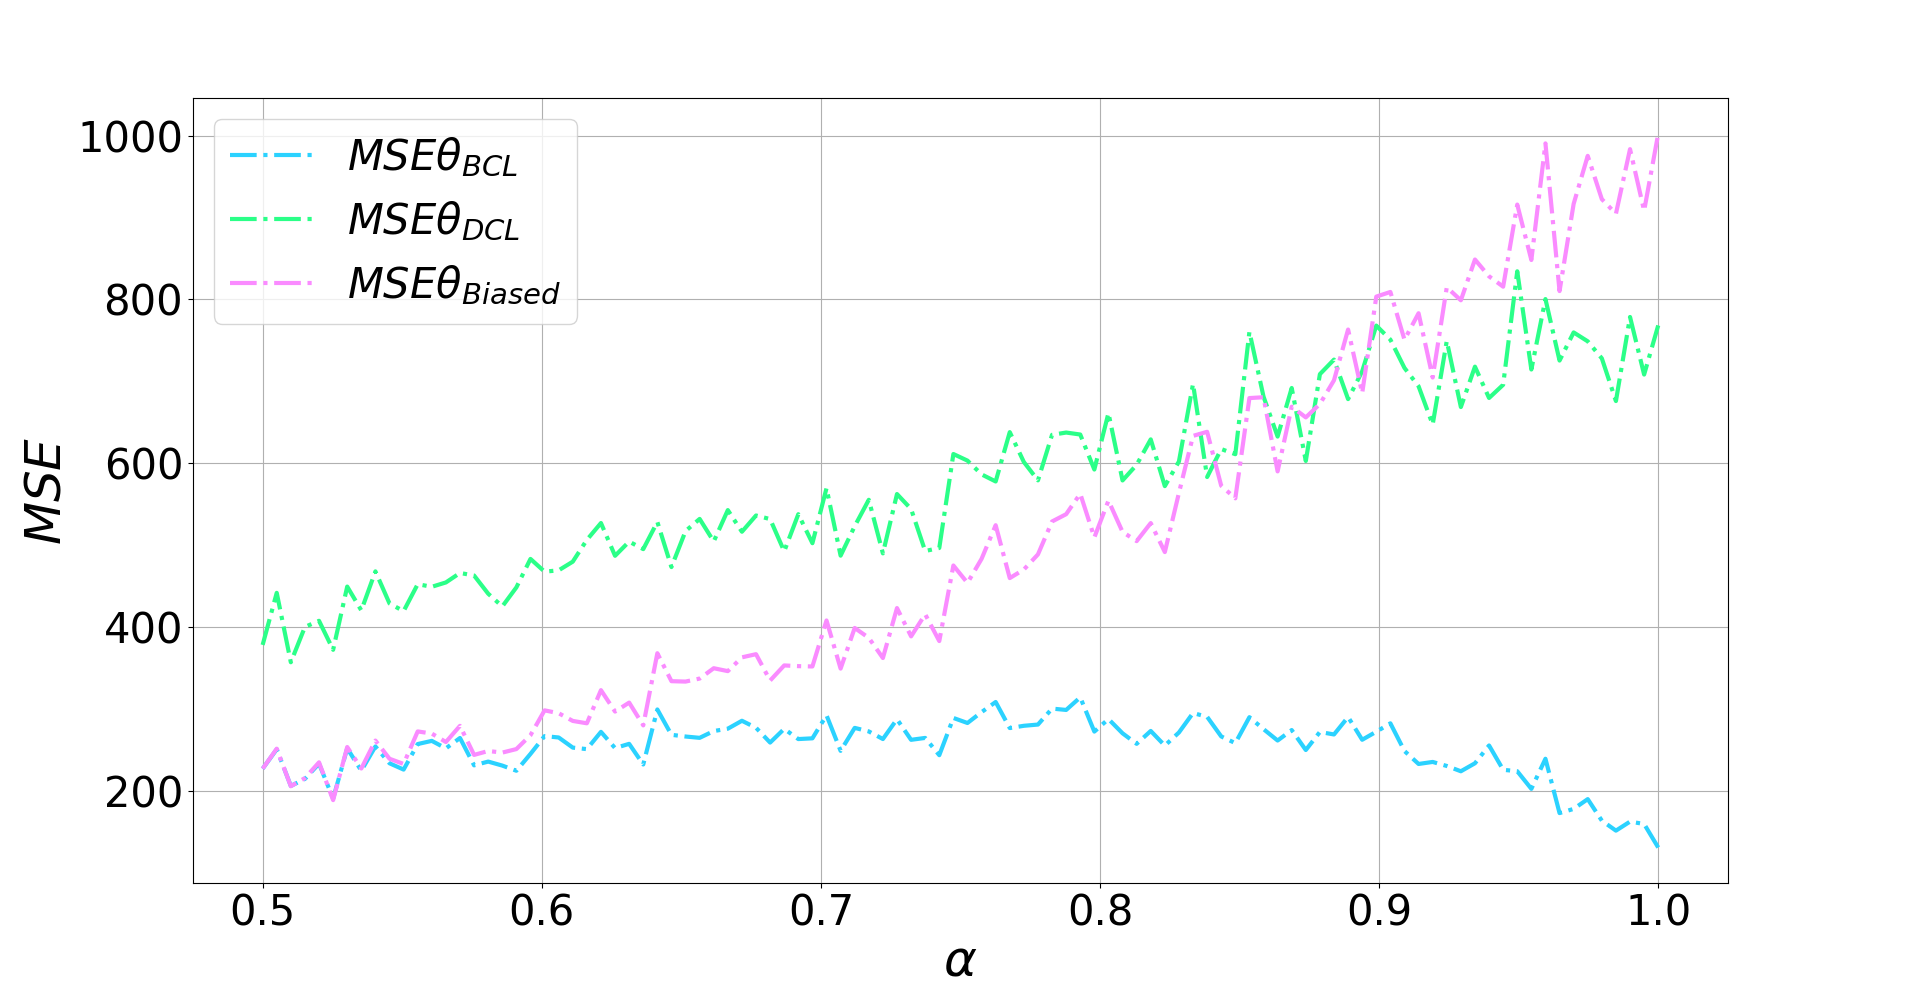
\includegraphics[width=0.5\textwidth, height=0.3\hsize]{numer_alpha.png}\label{fig:msealpha}}
	\subfloat[负例个数N的影响]
	{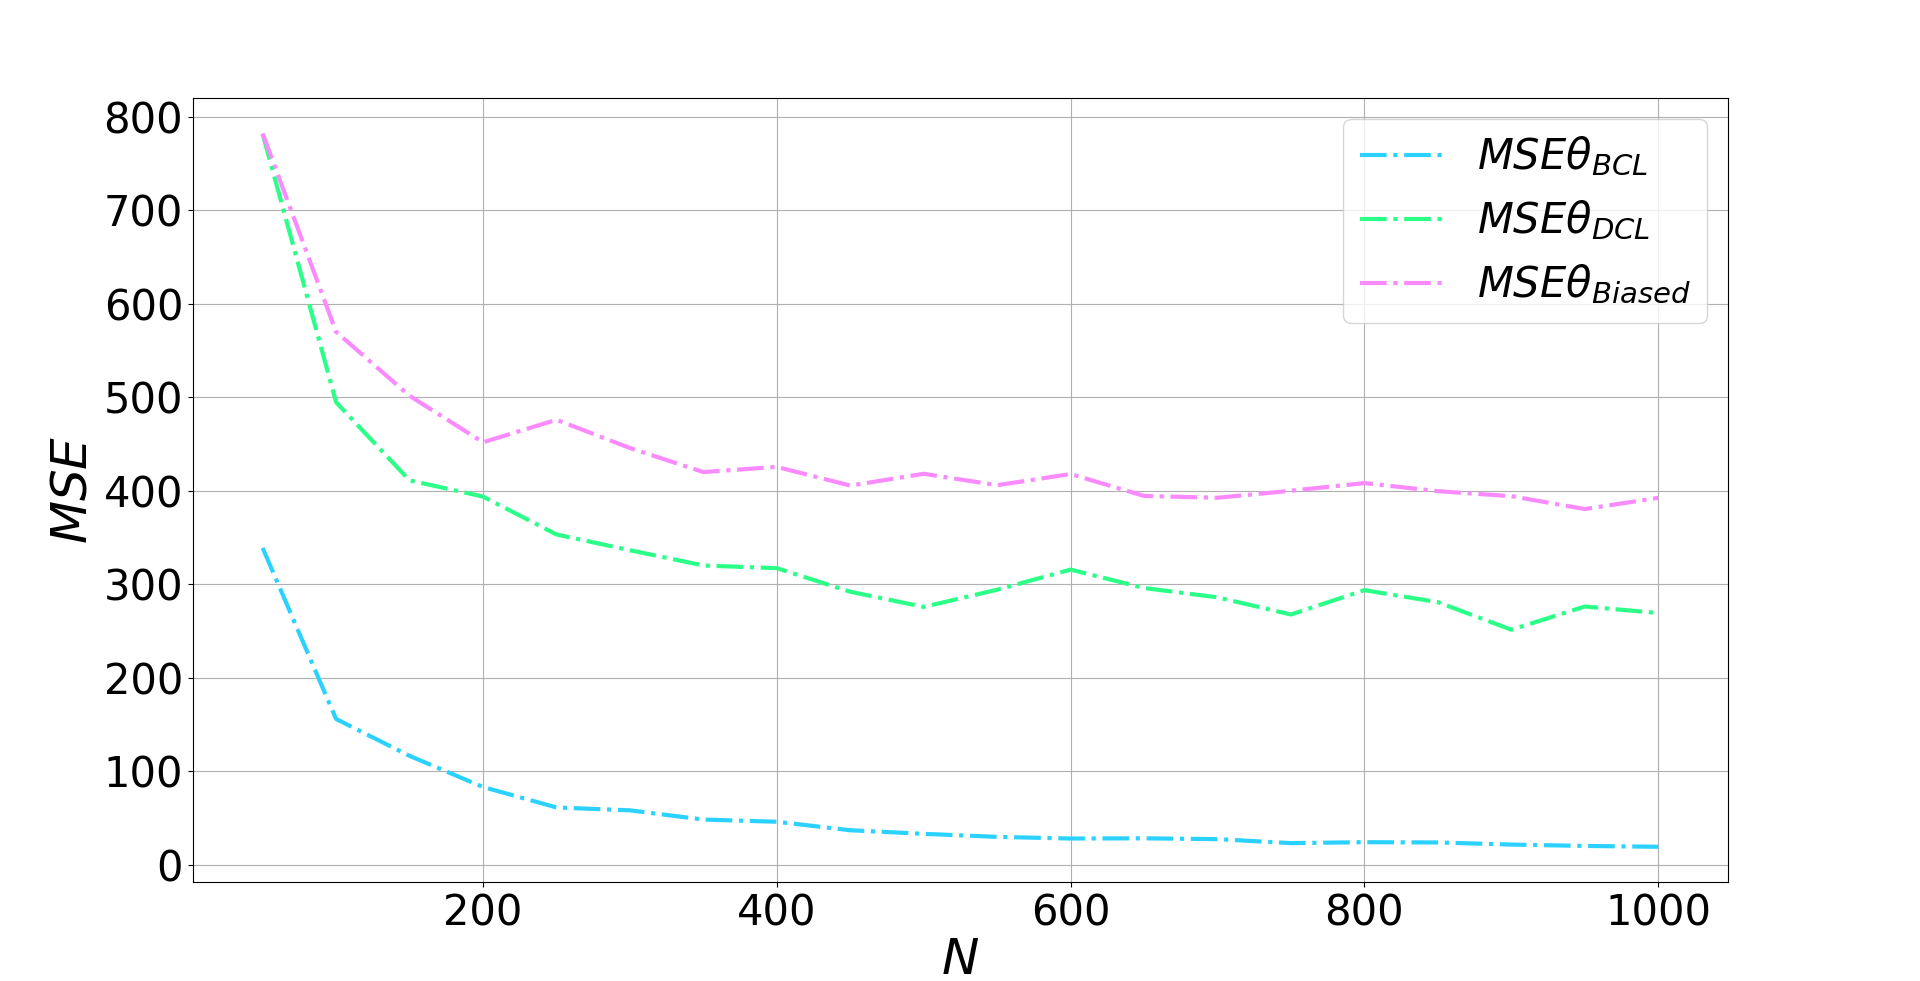
\includegraphics[width=0.5\textwidth, height=0.3\hsize]{numer_N.png}\label{fig:mseN}}\\
	\subfloat[类先验概率的影响]
	{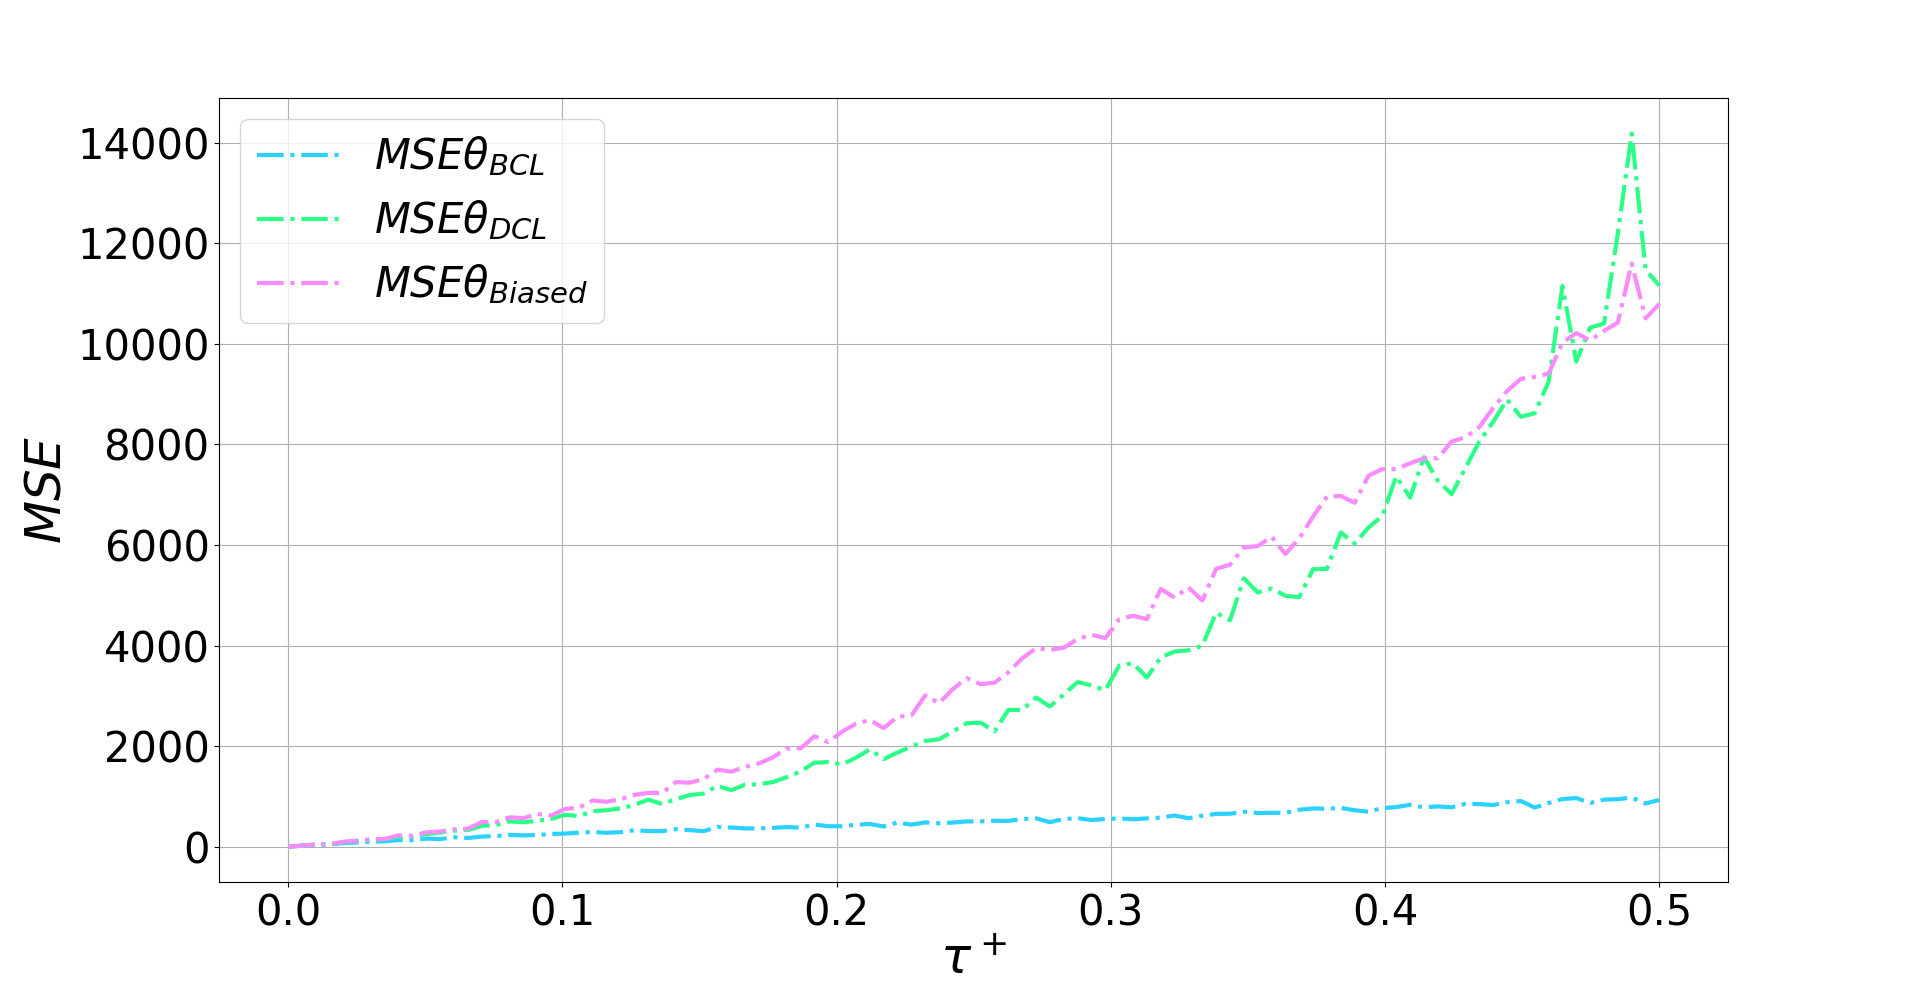
\includegraphics[width=0.5\textwidth, height=0.3\hsize]{numer_tau.png}\label{fig:msetau}}
	\subfloat[不同锚点的$\phi$变异程度的影响]
	{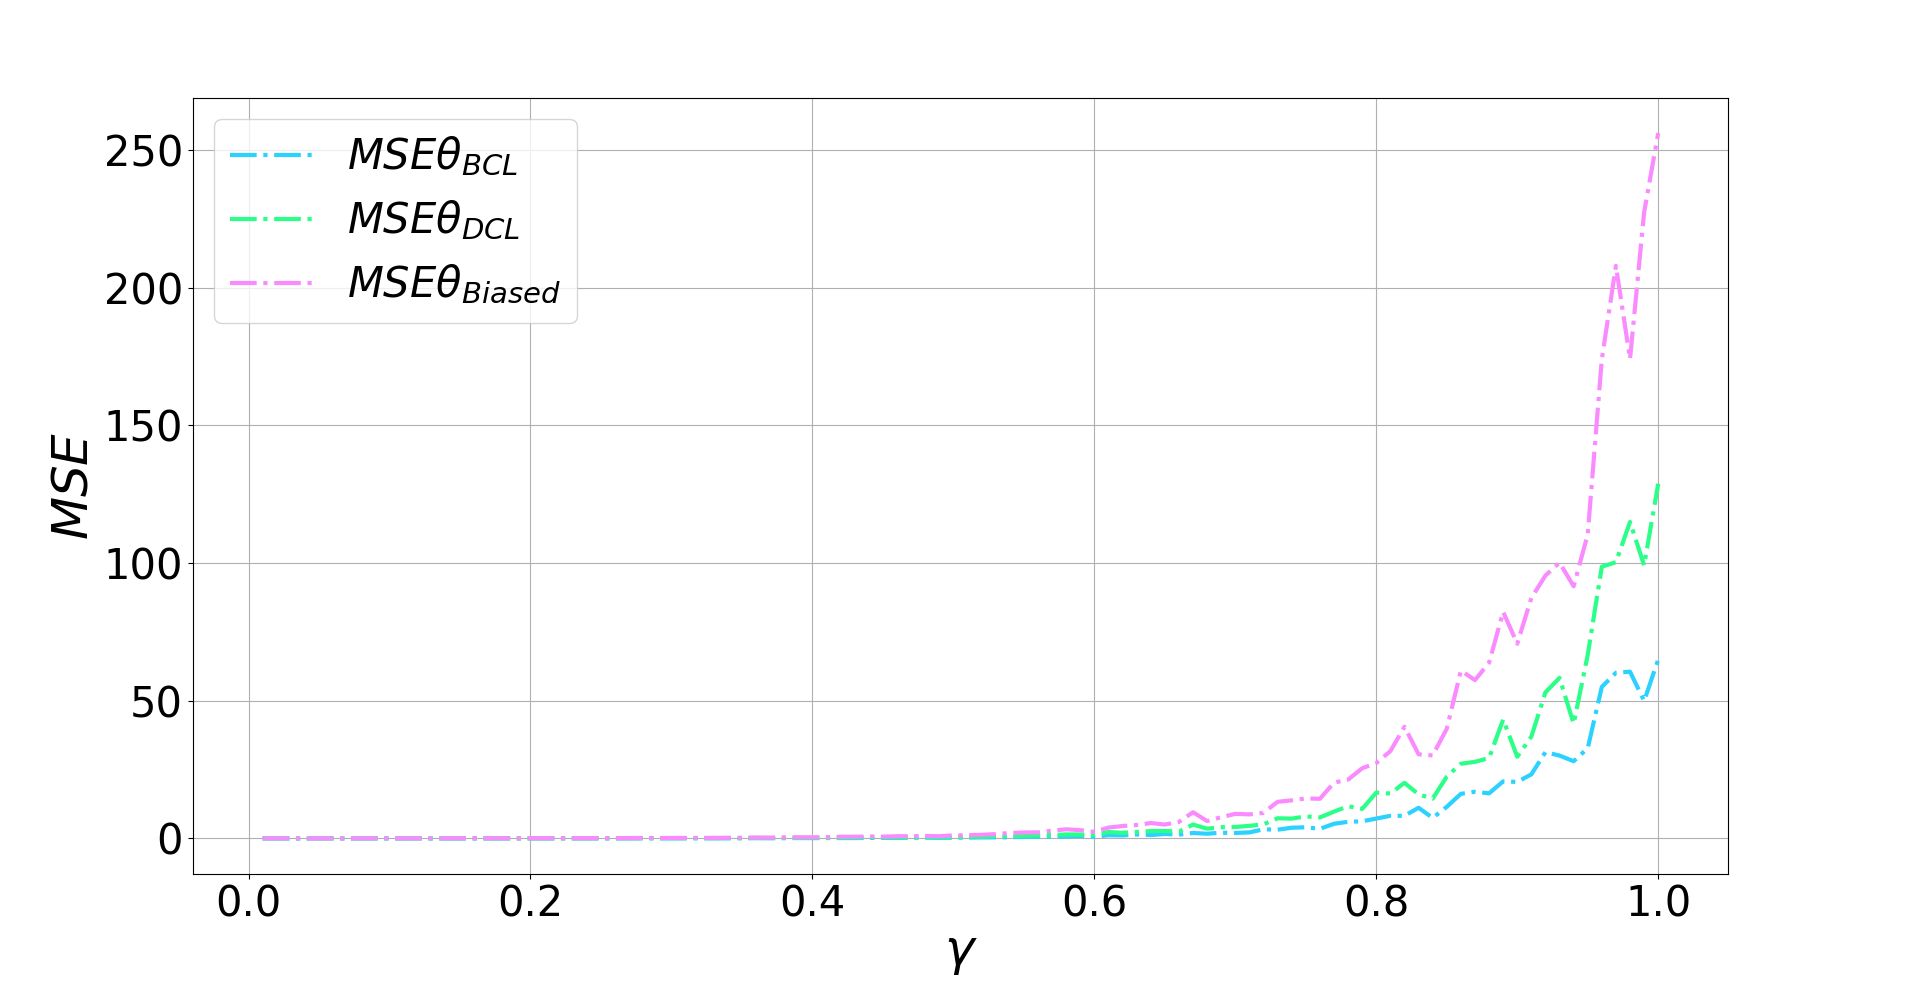
\includegraphics[width=0.5\textwidth, height=0.3\hsize]{numer_gamma.png}\label{fig:msegamma}}\\
	\subfloat[温度放缩系数$t$的影响]
	{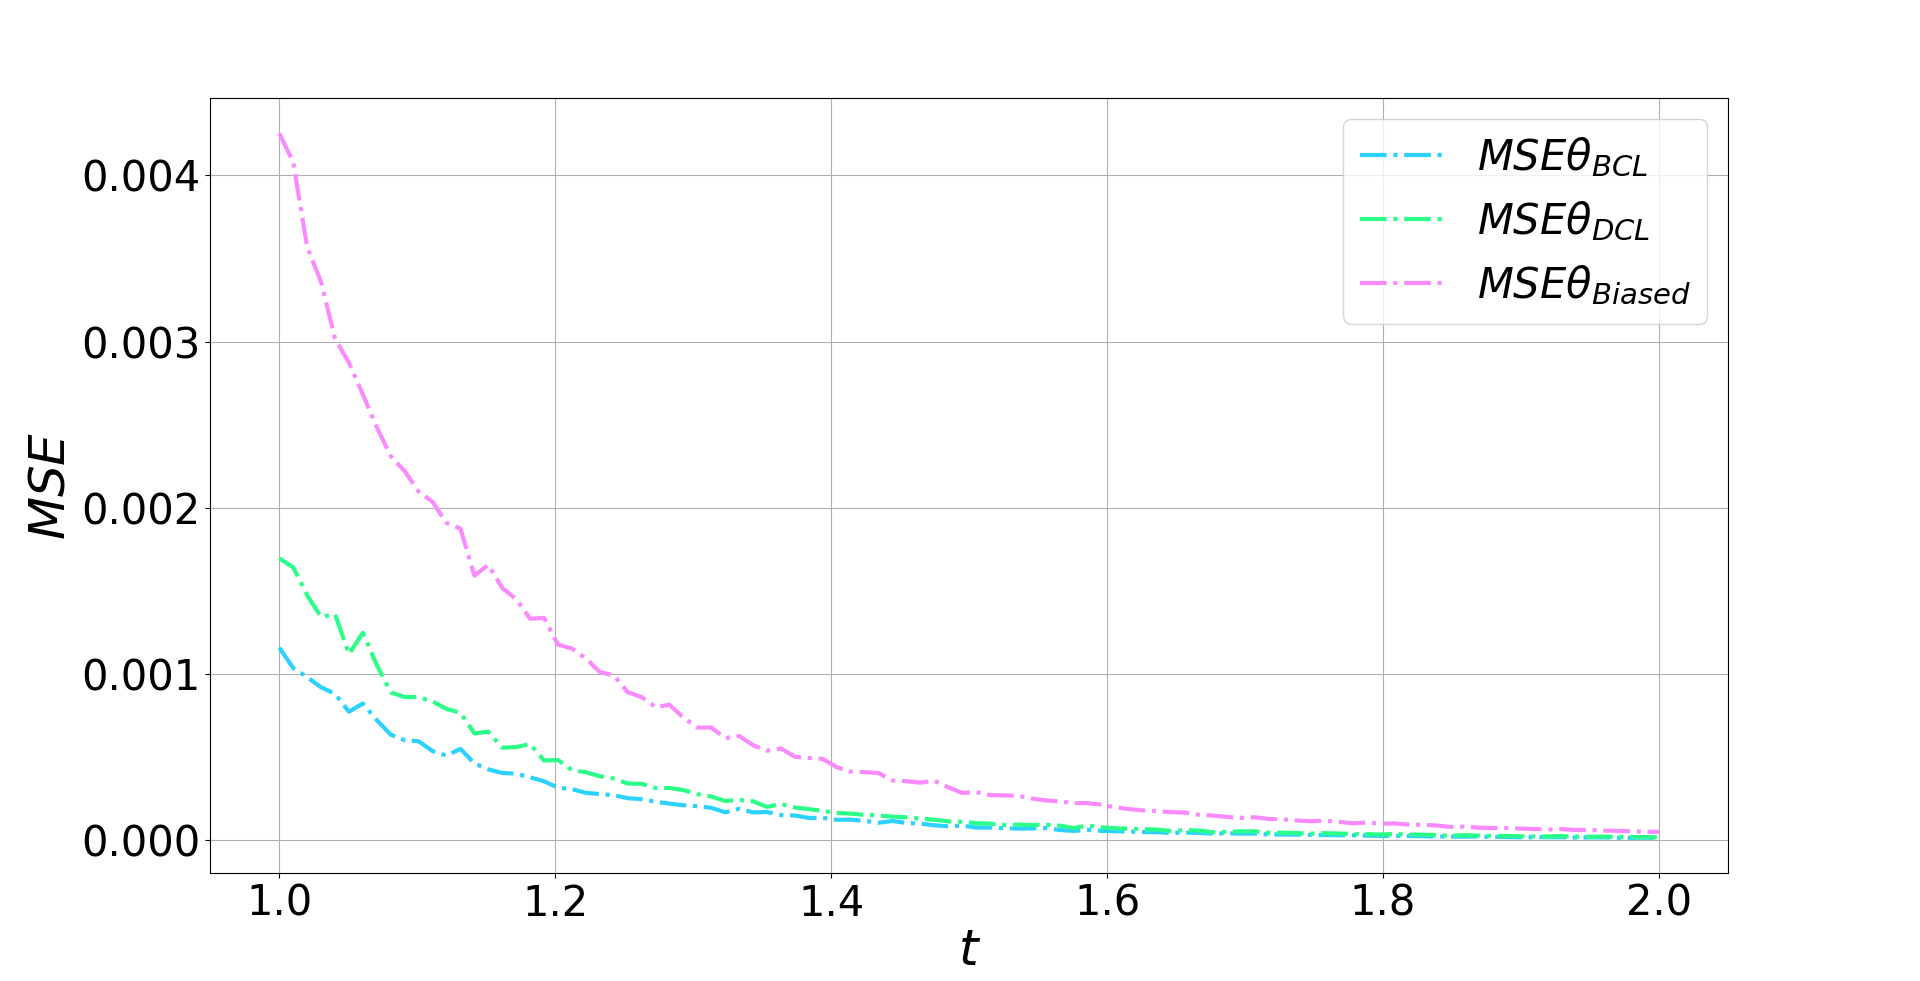
\includegraphics[width=0.5\textwidth, height=0.3\hsize]{numer_t.png}\label{fig:mset}}
	\subfloat[锚点数量M的影响]
	{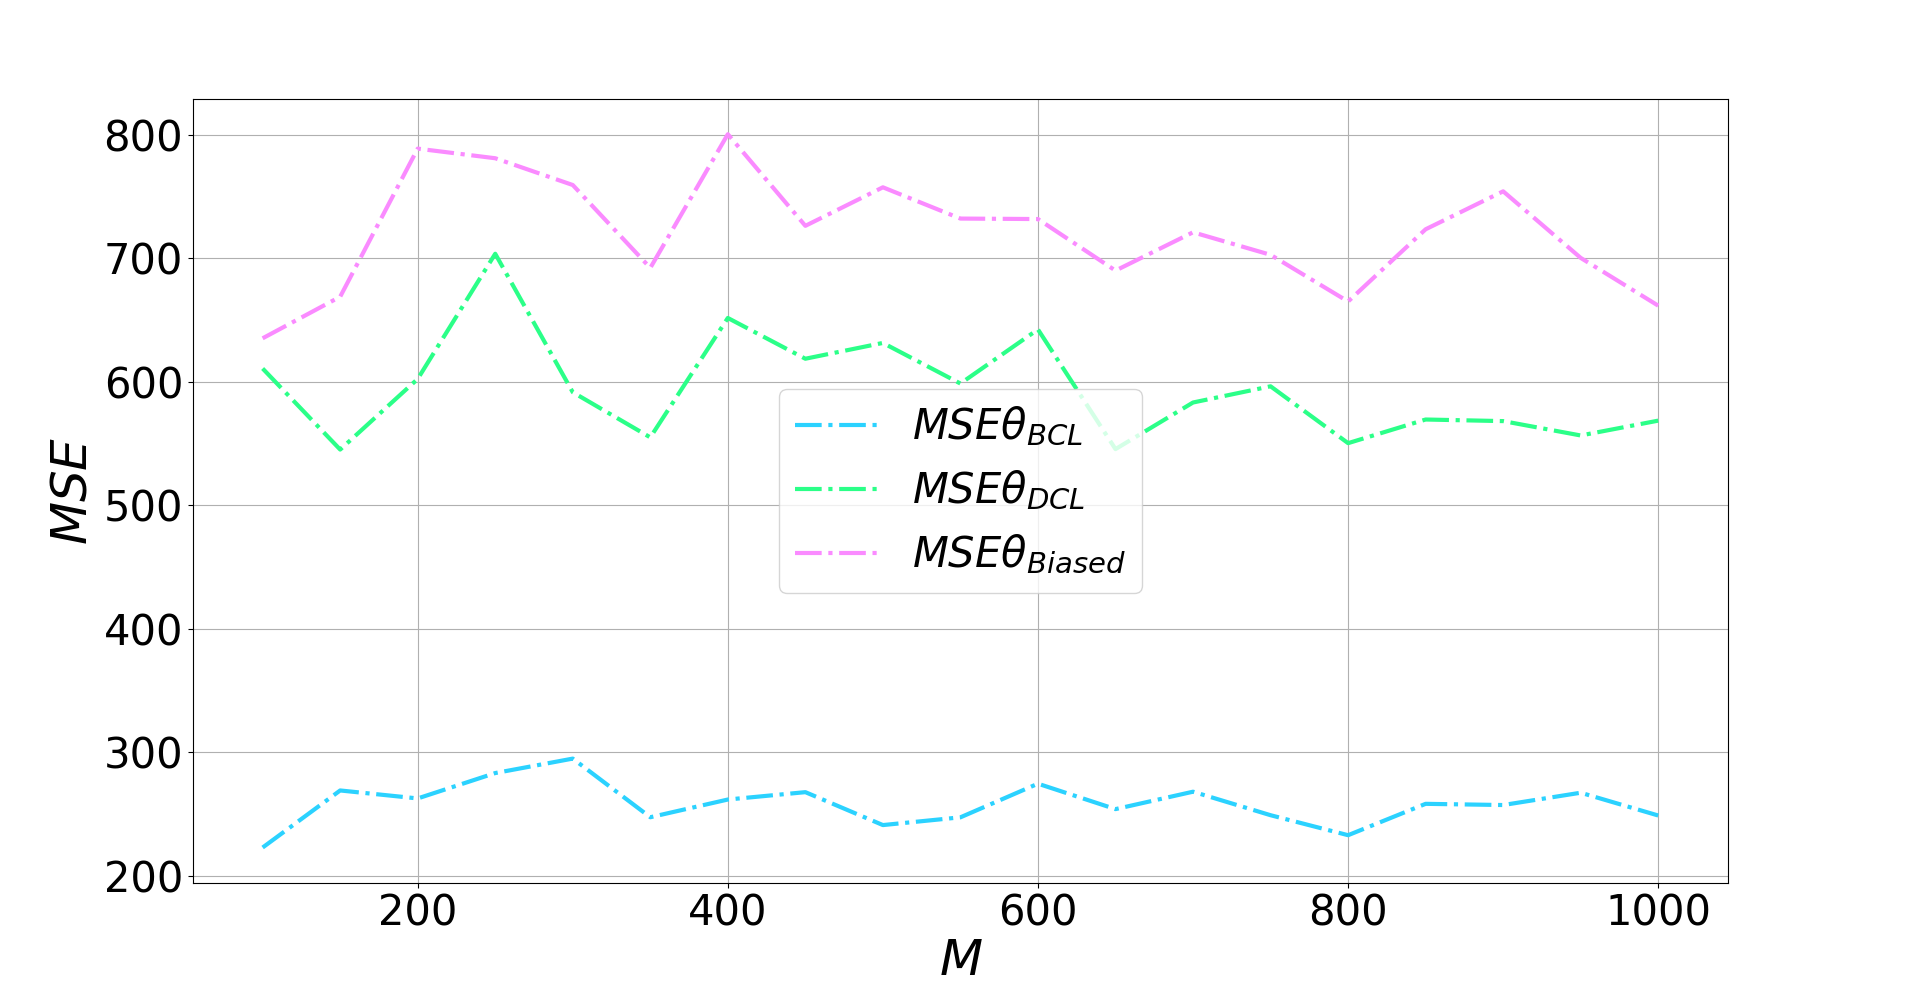
\includegraphics[width=0.5\textwidth, height=0.3\hsize]{numer_M.png}\label{fig:mseM}}
	\caption{不同参数设置下估计量的均方误差比较}
	\label{Fig:MSE}
\end{figure*}
%*******************************

%*******************************
\begin{figure}[h!]
	\centering
	\subfloat[]
	{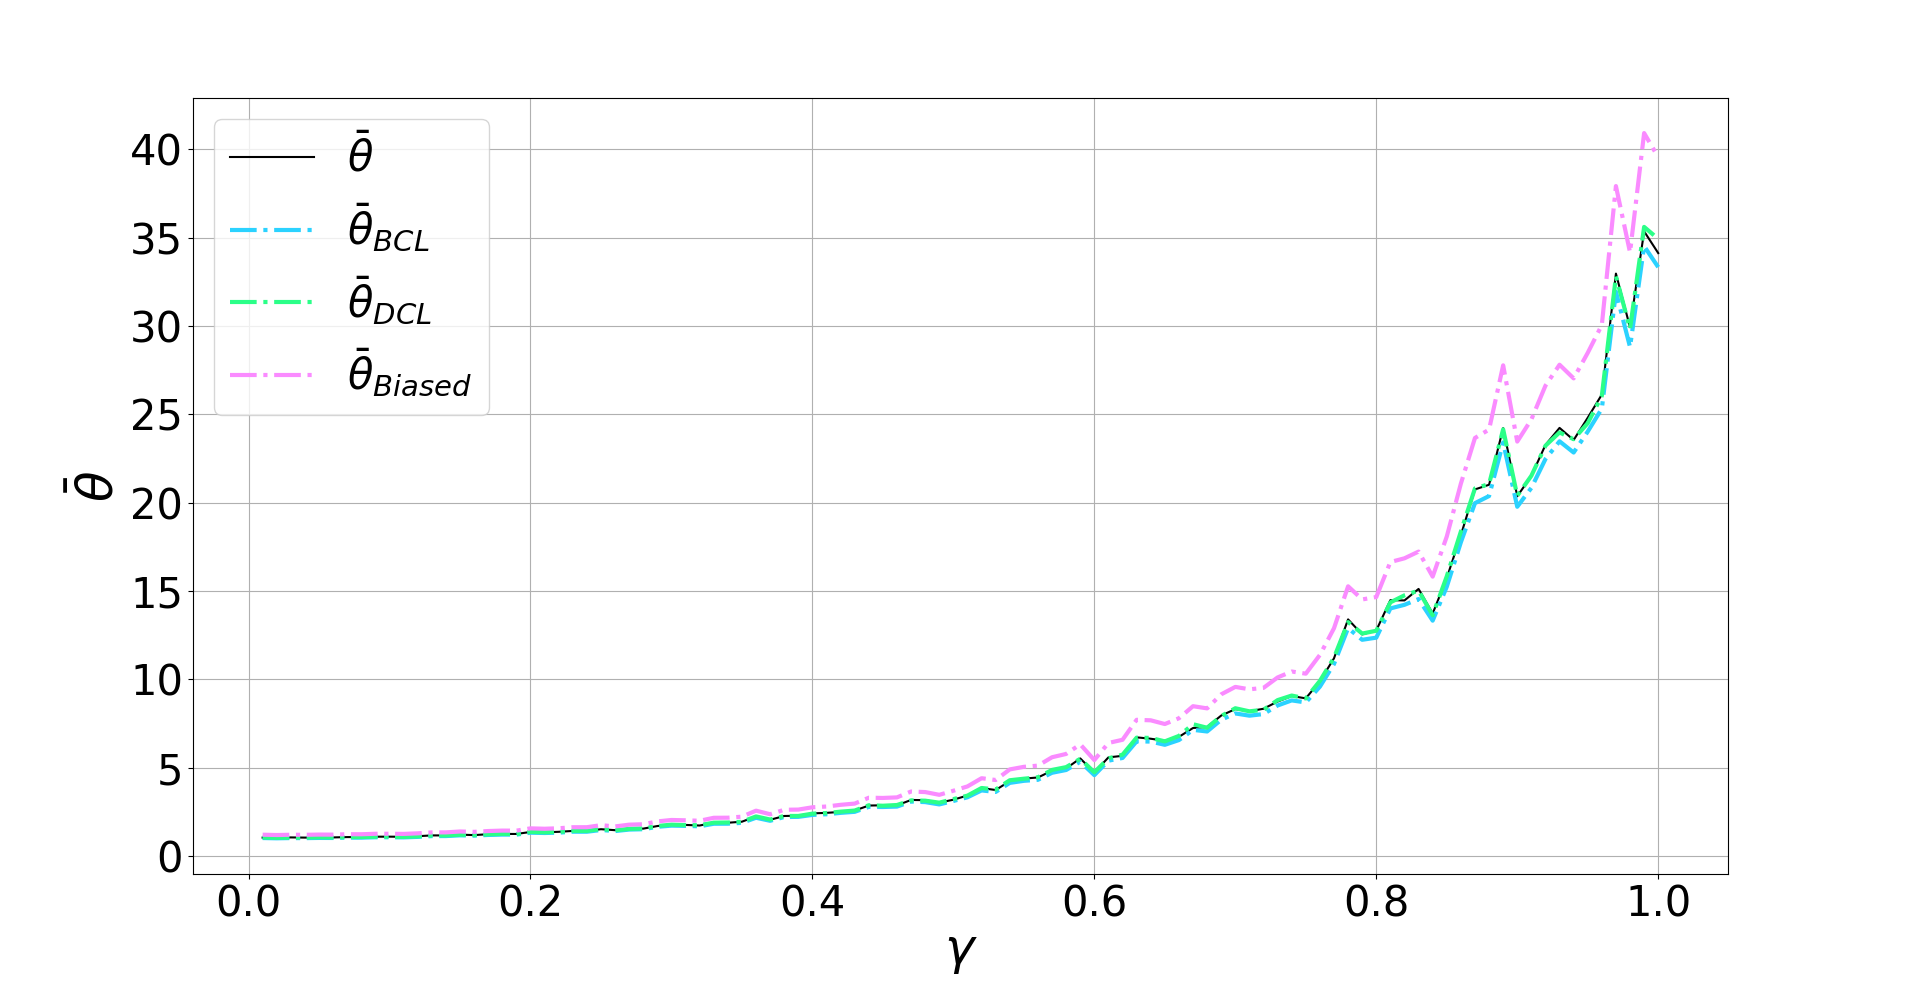
\includegraphics[width=0.49\textwidth, height=0.3\hsize]{numer_bargamma.png}\label{fig: numerbar_gamma}}\hspace{0.1cm}
	\subfloat[]
	{\includegraphics[width=0.49\textwidth, height=0.3\hsize]{numer_bar.png}\label{fig:numerbar_alpha}}
	\caption{不同参数设置下估计量的均值比较}
	\label{fig:numer_bar}
\end{figure}
%*******************************

\subsubsection{实验结果}
对于第$m$个锚点,可以计算得到真负例分数均值的真值,记为$\theta_{\textsc{Sup}, m}$;然后按照对比方法计算一个真负例分数的估计值,记为$\hat{\theta}_{m}$。进而,对于$M$个锚点,可以计算估计量的均方误差:
\[\textsc{Mse}\hat{\theta} = \frac{1}{M}\sum_{m=1}^M (\hat{\theta}_{m} -\theta_{\textsc{Sup}, m})^2 \]
首先固定参数设置如下:$\alpha=0.9$,$\gamma=0.1$,$\tau^+=0.1$,温度缩放$t=0.5$,锚点数量$M=1e3$,负样本数量$N=64$。然后变动不同的参数,统计不同估计量的均方误差。图\ref{Fig:MSE}对不同参数下不同估计量的均方误差MSE进行了比较。可以观察到,在不同的参数设置下,$\hat{\theta}_{\textsc{Bcl}}$估计量相对于其它估计量具有更低的均方误差。DCL方法主要受制于额外正样本得个数,在实践中,通常只有非常有限得额外正例个数可供使用。需要重点关注的是,随着负例个数N的增大,$\hat{\theta}_{\textsc{Bcl}}$的均方误差变小,与前面的分析一致。

除了MSE之外,图~\ref{fig:numerbar_alpha}还报告了不同估计量$\hat\theta$的均值在不同参数下的变化。受限于篇幅,重点关注分布$\phi$或编码器$f$的选择是否会影响估计器的一致性。图~\ref{fig: numerbar_gamma}显示了$\phi$变异对均值的影响。图~\ref{fig:numerbar_alpha}显示了编码器性能对均值的影响。
可以看到,$\hat\theta_\textsc{~Bcl}$、$\hat\theta_\textsc{~Dcl}$和$\theta$序列的均值非常接近,这是由切比雪夫大数定律保证的,即,当$\mathbb E ~\hat\theta_m = \theta_m$时,$\lim\limits_{M\rightarrow\infty} \mathbb{P}\{|\frac{1}{M}\sum_{m=1}^{M} \hat{\theta}_m-\frac{1}{M}\sum_{m=1}^{M} \theta_m |< \epsilon \} =1
$。这个结论不受建议分布$\phi$或编码器$f$的选择影响。$\hat\theta_\textsc{~Bcl}$、$\hat\theta_\textsc{~Dcl}$都是真负例分数均值的无偏估计量,这是重要性采样的性质以及均值估计量的性质决定的。此外,图\ref{fig:numerbar_alpha}也可以看作是训练过程的模拟:性能更好的编码器,即更高的$\alpha$,将真负样本编码得与锚点不相似(相似度分数更小),将正例编码得与锚点更近(相似度分数更大)。因此,观察到真负例分数均值$\bar\theta$的减少,对应于训练过程中损失值的减少,以及偏差$|\bar\theta_\textsc{Biased} -\bar\theta|$的增加,因为随着$\alpha$的增加,$\bar\theta_\textsc{Biased}$中包含的伪负样本得分更高。



\subsection{真实数据集实验}
\subsubsection{数据集}
在个性化推荐任务上,与第\ref{cha:fourthsection}章相同的五个公开数据集:MovieLens-100k,MovieLens-1M,Yahoo!-R3,Yelp2018和Gowalla。数据预处理方法也一样:前三个数据集包含用户评分,按照~\cite{Steffen:2009:UAI,Zhang:2013:SIGIR,Steffen:2014:WSDM} 的方法将所有有评分的物品转换为隐式反馈。对于每个数据集,随机将其中20\%的数据作为测试数据,剩下的80\%用于训练。数据集的统计信息可以参考第\ref{cha:fourthsection}章的实验部分。

在图像分类任务上,使用了四个公开数据集,CIFAR10,STL10,CIFAR100和tinyImageNet数据集。简单介绍CIFAR10数据集,CIFAR-10数据集包含10个类别的60000张尺寸为32x32的彩色图像,每个类别有6000张图像。其中,训练集包含50000张图像,测试集包含10000张图像。不同类别的训练样本完全互斥,且类比平衡。图\ref{Fig:cifar}提供了CIFAR10数据集的十个类别及相应的随机样本概览。其余三个数据集与CIFAR10数据集类似,都是类比平衡。除了STL10数据集以外,其他数据集都是完全标注的,但在训练过程中,训练集的标签都不使用,即负例无监督,仅在评估的时候使用类别标签。这四个数据集的统计信息如下表:
\begin{figure}[h!]
	\centering
	\includegraphics[width=0.7\textwidth]{cifar.png}
	\caption{CIFAR10数据集的十个类别及相应的随机样本概览}
	\label{Fig:cifar}
\end{figure}
\begin{table*}[h!]
	\centering
	\small
	\caption{图像分类任务数据集统计信息}\label{5Table:Dataset}
	\resizebox{1\textwidth}{!}{
	\begin{tabular}{lcccccc}
		\toprule[1.2pt]
		~           & 类比总数  & 图像尺寸  &训练集数量  &验证集数量&测试集数量&是否完全标注   \\ \cline{1-7}
		CIFAR10   &   10    &  32x32(RGB)   &50,000&   /	   & 10,000 &是\\
		STL10    &   10  &  96x96(RGB)  &105,000&  /     & 8,000&否  \\
		CIFAR100       &   100 &  32x32(RGB)  &50,000 &  /      & 10,000&是\\
		tinyImageNet       & 200&  64x64(RGB) &  100,000&   10,000&    10,000    & 是 \\
		\bottomrule[1.2pt]
	\end{tabular}
}
\end{table*}

\subsubsection{对比算法}
由于本章的出发点是通过对负样本加权校准估计,从而校准负例的梯度,不适用于两个网络分支分别采用梯度法和动量法更新的异步网络架构,因此对比方法仅考虑以LightGCN\cite{Xiangnan:2020:SIGIR}和SimCLR\cite{Chen:2020:ICML}为框架的同步法更新的网络架构,主要包含如下对比方法:

\begin{itemize}
	\item InfoNCE~\cite{Oord:2018:arxiv}:具体表达式见式\eqref{Eq:BiasLoss},在负例无监督场景下,该损失使用未标注样本的相似度分数替代真负例的相似度分数。
	\item DCL~\cite{Chuang:2020:NIPS}: 由于未标记数据中存在伪负例,DCL提出了一个估计量见式\eqref{5Eq:DCLEstimator}来修正InfoNCE损失分母中的第二项中真负例分数和的估计。 
	\item HCL~\cite{Robinson:2021:ICLR}: 使用了DCL的去偏框架的基础上,进一步使用每个随机选择的未标记样本的相似度分数加权进行困难样本挖掘。DCL是$\beta=0$时HCL的一个特例。
\end{itemize}
这些对比算法的含义在上一章章实验部分已有介绍,不再赘述。

\subsubsection{实验设置}
无论是个性化推荐任务还是图像分类任务,都是通过优化对比损失学习样本的表示,根据学到的表示进行下游排序或者分类任务,因此学习样本的表示也被称为“代理任务”(pretext task)。尽管下游任务的评估协议略有差异:推荐任务是根据用户表示的K近邻物品表示生成top-K推荐(即内积相似度高的物品),而图像分类任务是将学到的表示固定,然后训练一个线性分类器。但共同点是,学到的对比表示质量越好,即正例越对齐,负例越均匀,下游排序或者分类任务的泛化性能越好。

在推荐任务上,使用两个编码器:矩阵分解(MF)\cite{Koren:2009:Computer}和轻量级图卷积网络(LightGCN)\cite{Xiangnan:2020:SIGIR}。不同的推荐模型都会编码的用户和物品表示,然后计算对比损失以训练推荐模型。根据学到的用户物品表示,计算用户评分矩阵,从而为每个用户预测个性化推荐列表。评估指标与前面保持一致,包括精确度(P)、召回率(R)和归一化折损累积增益(NDCG),其中$K$的取值为5、10和20。

在图像分类任务方面进行公平的比较,所有实验设置与DCL~\cite{Chuang:2020:NIPS}和HCL~\cite{Robinson:2021:ICLR}完全相同。具体地,仅考虑同步同构的网络架构SimCLR\cite{Chen:2020:ICML}框架,它使用的是InfoNCE损失函数。不同的对比方法使用完全相同的数据增强方法,使用ResNet-50\cite{He:2016:CVPR}作为编码器架构,并使用学习率为0.001的Adam优化器~\cite{Adam:2015:ICLR}。温度缩放系数和潜在向量的维度分别固定为$t$=0.5和$d$=128,所有模型训练400个epochs。在评估上与推荐任务有所不同,图像分类任务的评估遵循已有的评估协议:首先固定学习到的嵌入,然后通过训练线性分类器进行评估~\cite{Lajanugen:2018:ICLR,Robinson:2021:ICLR},评估指标使用ACC。在训练时均不使用标签,只在评估精度时使用样本标签。

\subsection{实验结果}
\subsubsection{个性化推荐}
\begin{table*}[h!]
	\centering
	\caption{Top-k推荐性能比较}\label{5Table:Recommendation}
	\resizebox{1\textwidth}{!}{
		\begin{tabular}{lllccccccccccc}
			\toprule[1.2pt]
			\multirow{2}*{\textbf{数据集}} & \multirow{2}*{\textbf{模型}} & \multirow{2}*{\textbf{学习算法}} & \multicolumn{3}{c}{Top-5评估} &~& \multicolumn{3}{c}{Top-10评估}&~&\multicolumn{3}{c}{Top-20评估}\\ \cline{4-6} \cline{8-10} \cline{12-14}
			~ & ~ & ~ & Precision& Recall& NDCG& ~ &Precision& Recall& NDCG& ~ &Precision& Recall& NDCG \\ \hline
			
			\multirow{10}*{\textbf{MovieLens-100k}} & \multirow{5}*{\textbf{MF}} &  Info\_NCE &0.4081 & 0.1388 & 0.4324 & ~ & 0.3452 & 0.2266 & 0.4095 & ~ & 0.2793 & 0.3497 & 0.4118 \\
			~ & ~ & DCL &0.4168 & 0.1434 & 0.4458 & ~ & 0.3513 & 0.2291 & 0.4202 & ~ & 0.2835 & 0.3546 & 0.4207 \\ 
			~ & ~ & HCL  & 0.4263 & 0.1463 & 0.4539 & ~ & 0.3565 & 0.2323 & 0.426 & ~ & 0.2849 & 0.3564 & 0.4242 \\	
			~ & ~ &BCL(Proposed)    &0.4374 & 0.1552 & 0.4674 & ~ & 0.3658 & 0.2405 & 0.4380 & ~ & 0.2931 & 0.3588 & 0.4357 \\
			\cline{2-14}
			
			~ & \multirow{5}*{\textbf{LightGCN}}  & Info\_NCE & 0.3924 & 0.1343 & 0.4209 & ~ & 0.3349 & 0.2183 & 0.4006 & ~ & 0.2679 & 0.3289 & 0.3976 \\ 
			~ & ~ & DCL & 0.3962 & 0.1367 & 0.4243 & ~ & 0.3361 & 0.2194 & 0.4022 & ~ & 0.2695 & 0.3329 & 0.4006 \\ 
			~ & ~ & HCL & 0.4197 & 0.1461 & 0.4501 & ~ & 0.3458 & 0.2256 & 0.4188 & ~ & 0.2802 & 0.3446 & 0.4182 \\
			~ & ~ & BCL(proposed) & 0.4366 & 0.1512 & 0.4652 & ~ & 0.3626 & 0.2367 & 0.4351 & ~ & 0.2936 & 0.3599 & 0.4347 \\ \hline\hline
			
			
			\multirow{10}*{\textbf{MovieLens-1M}} & \multirow{5}*{\textbf{MF}} & InfoNCE & 0.3820 & 0.0879 & 0.4003 & ~ & 0.3339 & 0.1478 & 0.3728 & ~ & 0.2821 & 0.2358 & 0.3605 \\ 
			~ & ~ & DCL &  0.4009 & 0.0934 & 0.4209 & ~ & 0.3472 & 0.1546 & 0.3894 & ~ & 0.289 & 0.2423 & 0.3731\\ 
			~ & ~ & HCL & 0.4112 & 0.0969 & 0.4317 & ~ & 0.3552 & 0.1585 & 0.3991 & ~ & 0.2959 & 0.2475 & 0.3825 \\ 
			~ & ~ & BCL(proposed) & 0.4249 & 0.1041 & 0.4439 & ~ & 0.3652 & 0.1657 & 0.4101 & ~ & 0.3012 & 0.2537 & 0.3920 \\ 
			\cline{2-14}
			~ & \multirow{5}*{\textbf{LightGCN}} &InfoNCE & 0.4121 & 0.0986 & 0.4386 & ~ & 0.359 & 0.1594 & 0.4041 & ~ & 0.2979 & 0.2482 & 0.3869 \\ 
			~ & ~ & DCL & 0.4104 & 0.0982 & 0.4291 & ~ & 0.3544 & 0.1597 & 0.3977 & ~ & 0.2965 & 0.2511 & 0.3842 \\ 
			~ & ~ & HCL & 0.4107 & 0.0948 & 0.4300 & ~ & 0.3514 & 0.1542 & 0.3950 & ~ & 0.2916 & 0.2413 & 0.3775 \\ 
			~ & ~ & BCL(proposed) & 0.4256 & 0.1047 & 0.4460 & ~ & 0.3651 & 0.1658 & 0.1893 & ~ & 0.2998 & 0.2534& 0.3911 \\\hline \hline
			
			\multirow{10}*{\textbf{Yahoo!-R3}} & \multirow{5}*{\textbf{MF}} & Info\_NCE & 0.1429 & 0.1065 & 0.1615 & ~ & 0.1080 & 0.1601 & 0.1664 & ~ & 0.0786 & 0.2316 & 0.1952 \\ 
			~ & ~ & DCL &0.1454 & 0.1083 & 0.1635 & ~ & 0.1091 & 0.1618 & 0.1692 & ~ & 0.079 & 0.2327 & 0.1974  \\ 
			~ & ~ & HCL & 0.1460 & 0.1097 & 0.1638 & ~ & 0.1096 & 0.1628 & 0.1697 & ~ & 0.0792 & 0.2336 & 0.1976 \\ 
			~ & ~ & BCL(proposed) & 0.1529& 0.1122 & 0.1685 & ~ & 0.1124 & 0.1667 & 0.1736 & ~ & 0.0815 & 0.2367 & 0.2029 \\ 
			\cline{2-14}
			~ & \multirow{5}*{\textbf{LightGCN}} & Info\_NCE & 0.1417 & 0.1074 & 0.1676 & ~ & 0.1099 & 0.1633 & 0.1719 & ~ & 0.0798 & 0.2354 & 0.2007  \\ 
			~ & ~ & DCL & 0.1456 & 0.1092 & 0.1642 & ~ & 0.1089 & 0.1622 & 0.1697 & ~ & 0.079 & 0.2333 & 0.1982\\ 
			~ & ~ & HCL & 0.1412 & 0.1139 & 0.1718 & ~ & 0.113 & 0.1683 & 0.1776 & ~ & 0.0812 & 0.2394 & 0.2059 \\ 
			~ & ~ & BCL(proposed) & 0.1537 & 0.1140 &  0.1725 & ~ & 0.1156 & 0.1696  & 0.1771 & ~ & 0.0842 & 0.2428 & 0.2076\\ \hline\hline
			
			
			\multirow{10}*{\textbf{Yelp2018}} & \multirow{5}*{\textbf{MF}} & Info\_NCE  & 0.0429 & 0.0246 & 0.047 & ~ & 0.0365 & 0.0417 & 0.0491 & ~ & 0.0305 & 0.07 & 0.058 \\ 
			~ & ~ & DCL & 0.0486 & 0.0278 & 0.0531 & ~ & 0.0410 & 0.0466 & 0.0552 & ~ & 0.0342 & 0.0777 & 0.0648 \\
			~ & ~ & HCL & 0.0515 & 0.0305 & 0.0566 & ~ & 0.0459 & 0.0541 & 0.0622 & ~ & 0.0383 & 0.0894& 0.0736 \\ 
			~ & ~ & BCL(proposed) & 0.0546 & 0.0342 & 0.0595 & ~ & 0.0475 & 0.0563 & 0.0643 & ~ & 0.0398 & 0.0912 & 0.0752 \\
			\cline{2-14}
			~ & \multirow{5}*{\textbf{LightGCN}} & Info\_NCE & 0.0553 & 0.0329 & 0.0607 & ~ & 0.0473 & 0.0558 & 0.0642 & ~ & 0.0390 & 0.0911 & 0.0754 \\ 
			~ & ~ & DCL & 0.0559 & 0.0331 & 0.0612 & ~ & 0.0472 & 0.0557 & 0.0642 & ~ & 	0.0391 & 0.0914 & 0.0756 \\ 
			~ & ~ & HCL & 0.0563 & 0.0335 & 0.0617 & ~ & 0.0477 & 0.0564 & 0.0648 & ~ & 0.0393 & 0.0920 & 0.0760 \\  
			~ & ~ & BCL(proposed) & 0.0612 & 0.0376 & 0.0670 & ~ & 0.0524 & 0.0629 & 0.0701 & ~ & 0.0414 & 0.1014 & 0.0815 \\\hline\hline
			
			
			\multirow{10}*{\textbf{Gowalla}} & \multirow{5}*{\textbf{MF}} & Info\_NCE & 0.0739 &0.0757 & 0.1016 & ~ & 0.0560 & 0.1122 & 0.1076 & ~ & 0.0422 & 0.1650 & 0.1230\\ 
			~ & ~ & DCL & 0.0746 & 0.0769 &0.1023 & ~ & 0.0568 & 0.1147 & 0.1088 & ~ & 0.0426 & 0.1664 & 0.1238 \\ 
			~ & ~ & HCL & 0.0755 & 0.0774 & 0.1035 & ~ & 0.0574 & 0.1151 & 0.1098 & ~ & 0.0432& 0.1693 & 0.1256 \\ 
			~ & ~ & BCL(proposed) & 0.0827 & 0.0837 & 0.1121 & ~ & 0.0639 & 0.1257& 0.1186 & ~ & 0.0485 & 0.1824 & 0.1353 \\
			\cline{2-14}
			~ & \multirow{5}*{\textbf{LightGCN}} & Info\_NCE & 0.0743 & 0.0760 & 0.1022 & ~ & 0.0566 & 0.1132& 0.1084 & ~ & 0.0423 & 0.1649 & 0.1231\\ 
			~ & ~ & DCL & 0.0748 & 0.0763 & 0.1027 & ~ & 0.0569 & 0.1132 & 0.1088 & ~ & 0.0424 & 0.1656 & 0.1236 \\ 
			~ & ~ & HCL & 0.0794 & 0.0804 & 0.1084 & ~ & 0.0608 &0.1199 & 0.1147 & ~ & 0.0453 & 0.1740 & 0.1319 \\ 
			~ & ~ & BCL(proposed) & 0.0863 &  0.0893 & 0.1156 & ~ &  0.0670 &  0.1332 & 0.1248 & ~ & 0.0490 & 0.1937 & 0.1420  \\ \hline
			\bottomrule[1.5pt]
			
		\end{tabular}
	}
\end{table*}
表\ref{5Table:Recommendation}提供了不同的学习算法在五个数据集上的top-k性能评估。含有去偏机制的DCL方法普遍由于有偏的InfoNCE方法,表明在positive-unlabeled的隐式反馈数据集上进行伪负例去偏是必要的,这个结论与前面章节结论一致。此外,包含硬负例挖掘机制的HCL方法和BCL方法普遍由于不含硬负例挖掘机制的DCL和InfoNCE方法,说明在隐式反馈数据集上进行硬负例挖掘的必要性。

需要着重强调的是HCL和BCL的差别,它们都包含困难负例挖掘和伪负例去偏机制,但是BCL显著优于HCL方法。这是由于两者重要性加权机制的不同所造成的:HCL的权重可以简单理解为未标注样本相似度分数的指数次方,相似度分数越大,重要性权重越大,可以很好的兼顾硬负例挖掘任务,但无法兼顾伪负例去偏任务;BCL的权重是未标注样本是真负例的后验概率,可以灵活地兼顾硬负例挖掘和伪负例去偏任务。此外,HCL的权重是样本相似度分数的函数,而BCL的权重是经验分布函数(相对排序位置)的函数。在推荐中,嵌入倾向于过度平滑,从而导致相似度分数趋同,那么HCL的权重可能会消失。而BCL的权重不会受到相似度分数具体值的影响,因此表现出了更好的鲁棒性。

\subsubsection{图像分类}
前面讨论了,应该在显存可承受的范围内,设定尽量大的负例个数N值。以24GB显存的RTX3090显卡为例,能够承受的最大的N=510,此时批量大小为256(在SimCLR框架下,负例个数N=2*batch size -2)。固定N=510,然后使用不同的方法训练。其中,在CIFRA10数据集上,$\alpha$是通过经验评估计算的,$\beta=0.9$;在STL10数据集上,设定$\alpha=0.75$,$\beta=1.0$;在STL10数据集上,设定$\alpha=0.7$,$\beta=1.0$;在TinyImageNet数据集上,设定$\alpha=0.8$,$\beta=1.0$;可以看到,BCL相对于对于SimCLR,top-1分类精度分别取得了1.4%,6.3%,3.3%和3.9%的绝对提升。相对于最优对比方法HCL,BCL的top-1分类精度分别取得了0.6%,0.1%,0.2%和0.3%的绝对提升,在CIFAR10和TinyImagenet数据集上的提升具有显著性。

\begin{table}[h!]
	\centering
	\caption{Top-1图像分类精度比较}\label{Exp:acc}
	\resizebox{0.8\textwidth}{!}{
		\begin{tabular}{lcccccc}
			\toprule[1.2pt]
			
			数据集&负例个数N &模型& SimCLR & DCL & HCL & BCL  \\ \hline
			CIFAR10 & 510 &ResNet50& 91.1   &92.1	&91.9	&\textbf{92.5}($\pm 0.15$) \\
			STL10& 510 &ResNet50& 80.2   &84.3	&87.4	&\textbf{87.5}($\pm 0.12$)\\
			CIFAR100& 510&ResNet50 & 66.4   &67.7	&69.5	&\textbf{69.7}($\pm 0.10$)\\
			tinyImageNet& 510&ResNet50 & 53.4   &53.7	&57.0	&\textbf{57.3}($\pm 0.09$)\\
			\cline{1-7}
			\bottomrule[1.2pt]
			
		\end{tabular}
	}
\end{table}

\subsection{超参数分析}
由于图像数据集上标注比较完备,而推荐数据集始终存在未标注样本,因此使用图像数据集分析不同超参数的影响。

\textbf{负例个数N的影响}:首先固定$\alpha$和$\beta$的值如上所述,然后分析不同负例个数N对分类精度的影响。结果如表\ref{Exp:result}所示,对于所有的对比方法,更大的负例个数N导致了分类精度一致的提升。这与对比损失本身的性质有关,更大的N导致了更大的互信息下界。此外,对于HCL方法而言,更大的N导致(1)经验分布函数$\hat{\Phi}_\textsc{Un}(\hat{x})$的估计误差减小;(2) $\alpha$的估计误差减小;(3)重要性采样的估计误差减小,从而使得BCL经验估计的估计误差确定性地减小,这与数值实验部分的结论是一致的。
\begin{table}[h!]
	\centering
	\caption{负例个数的影响}\label{Exp:result}
	\resizebox{0.8\textwidth}{!}{
		\begin{tabular}{cclcccc}
			\toprule[1.2pt]
			\multirow{2}*{数据集} &  \multirow{2}*{学习算法} & \multicolumn{5}{c}{负例个数N} \\\cline{3-7}
			
			~ & ~ & N=30 & N=62& N=126& N=254&N=510 \\ \hline
			
			\multirow{4}*{\textbf{CIFAR10}} & SimCLR & 80.21 & 84.82   &87.58&89.87	&91.12\\
			~&DCL& 82.41 & 87.60   &90.38	&91.36	&92.06\\
			~&HCL& 83.42 & 88.45   &90.53	&91.57	&91.92\\
			~&BCL& 83.61 & 88.56   &90.83	&92.07	&92.58\\
			\cline{1-7}
			
			\multirow{4}*{\textbf{STL10}} & SimCLR & 61.20 & 71.69   &74.36	&77.33	&80.20\\
			~&DCL& 63.91 & 71.48   &76.69	&81.48	&84.26\\
			~&HCL& 67.24 & 73.38   &79.44	&83.82	&86.38\\
			~&BCL& 67.45 & 73.36   &80.23	&84.68	&86.51\\
			\cline{1-7}
			\bottomrule[1.2pt]
			
		\end{tabular}
	}
\end{table}


\begin{table}[h!]
	\centering
	\caption{参数$\beta$的影响}\label{Exp:beta}
	\resizebox{0.8\textwidth}{!}{
		\begin{tabular}{cclcccc}
			\toprule[1.2pt]
			
			\textbf{Dataset} & $\beta=0.5$ & $\beta=0.6$ & $\beta=0.7$ & $\beta=0.8$ & $\beta=0.9$ &$\beta=1.0$  \\ \hline
			\textbf{CIFAR10}&91.39 & 91.41 & 91.89   &92.02	&\textbf{92.58}	&92.12\\
			\textbf{STL10}&80.32& 81.79 & 83.58   &83.83	&84.85	&\textbf{86.51}\\
			\cline{1-7}
			\bottomrule[1.2pt]
			
		\end{tabular}
	}
\end{table}

\textbf{$\beta$的影响}:$\alpha$对应于编码器的宏AUC,有明确的含义;而$\beta$控制着采样分布的难度级别(hardness level),是手动选择的,因此只分析参数$\beta$的影响。固定最优参数$\alpha$不变,然后检查不同$\beta$值的影响。表~\ref{Exp:beta}展示了难度级别$\beta$的影响。在STL10数据集上,随着$\beta$的增加,Top-1分类准确率持续提高。然而,在CIFAR10数据集上,随着$\beta$的增加,Top-1分类准确率逐渐增加,在0.9处达到最优值后开始下降。这结果表明,更高的难度级别并不总是导致更好的性能。这一观点也可以从HCL和DCL的性能比较得到印证,HCL(包含困难负样本挖掘机制)在CIFAR10数据集上的表现比DCL(不包含困难负样本挖掘机制)要差。

如何设定一个合理的硬负例挖掘参数$\beta$?关于深度神经网络的记忆效应的研究~\cite{Arpit:2017:ICML}为回答这个问题提供了启发。具体而言,已经证明,不论使用何种网络架构,深度模型会优先记忆带有干净标签的训练数据,并随着训练轮数的增加逐渐适应带有噪声标签的训练数据~\cite{zhang2021understanding, Han:2018:NIPS}。自监督对比学习可以被视为一个负例含有噪声的噪声标签学习(noisy label learning)问题。较大的$\beta$值会导致给困难样本分配更高的权重,从而导致更大的损失值和相应的梯度值。为了避免神经网络拟合噪声,在正类先验较小的数据集(即噪声比较低的数据集)中,设置较大的β值可以加快对干净的困难样本的拟合,因此一个启发式的$\beta$设定值可以为
\[\beta = 1-1/C\]
其中,C为数据集的类别总数,那么1/C即为噪声率,越小的噪声率,那么应该设定一个更接近于1的$\beta$值。真是数据集的实验也验证了这个结论:在100类的CIFAR100和200类的tinyImageNet数据集上,最优的参数值为1。除了噪声率以外,另外一个需要考虑的因素是数据集本身拟合的难易度水平。与CIFAR-10数据集相比,STL-10数据集具有更大的挑战,它的top-1分类精度显著低于CIFAR10。因此,在相对难以拟合的STL-10数据集中,应当使用较大的$\beta$值可以激励神经网络在拟合噪声样本之前先拟合干净的困难样本。在相对容易拟合的CIFAR-10数据集中,应当使用相对小一点的$\beta=0.9$,避免神经网络拟合噪声样本。

\begin{table}[h!]
	\centering
	\caption{正例类先验概率$\tau^+$的影响}\label{Exp:tau}
	\resizebox{0.5\textwidth}{!}{
		\begin{tabular}{clccc}
			\toprule[1.2pt]
			数据集&	N &$\tau^+$	&	top1&	top5 \\\hline
			tinyImageNet&	510	&1e-3&	57.10&	80.54\\
			tinyImageNet&	510&	5e-3&	57.32&	80.87\\
			tinyImageNet&	510&	1e-2&	56.34&	80.24\\
			\cline{1-5}
			\bottomrule[1.2pt]
		\end{tabular}
	}
\end{table}

\textbf{$\tau^+$的影响}:表\ref{Exp:tau}展示了正例类先验概率$\tau^+$的设置对分类精度的影响。结果显示最佳的$\tau^+ = 1/C$。考虑数据集中的一个特定类别,比如"猫",可以将属于猫类的图像数量记为随机变量$X$,它可以看作N次独立成功率为$\tau^+$伯努利试验的结果,那么 $X\sim B(Y,\tau^+)$,其中$Y$是数据集中的所有样本数。在这种情况下,$\tau^+$的无偏估计$X/Y$。在一个平衡的数据集中,数据集中的总样本数为$Y = C * X$,其中$C$是类别的数量,$X$是每个类别中的样本数,于是有$\tau^+ = 1/C$。

\subsection{运行时间比较}
前面分析了,本章的方法的额外计算开销主要是由于经验分布函数的计算,其复杂度为O(N),其中N = 2 * (batch size-1),相比于编码一个样本,这个开销是可以忽略的。表\ref{Exp:time}比较了在不同数据集上进行单个训练周期的实际运行时间。其中,批量大小固定为256,编码器架构为ResNet-50。在CIFAR10、STL10和CIFAR100数据集上的实验是在配备了Intel(R) Xeon(R) Platinum 8255C CPU和单卡的RTX 3090(24GB) * 1 GPU的云服务器上进行的。在tinyImageNet数据集上的实验是在配备了Intel(R) Xeon(R) Platinum 8352M CPU和单卡的A100-SXM4-80GB(80GB) * 1 GPU的云服务器上进行的。结果显示,本章提出的方法几乎相比于对比方法有着相同的运行时间。tinyImageNet数据集运行时间较长是因为图像增强模块中,随机剪裁后图像的尺寸相对于前面三个数据集更大。
\begin{table}[h!]
	\centering
	\caption{算法运行时间比较}\label{Exp:time}
	\resizebox{0.4\textwidth}{!}{
		\begin{tabular}{clcc}
			\toprule[1.2pt]
			数据集&	Batch Size&	SimCLR&		BCL \\ \hline
			CIFAR10	&256&	82s	&	82s\\
			STL10&	256	&169s	&	169s\\
			CIFAR100&	256	&82s&	82s\\
			tinyImageNet&	256&	237s&238s\\
			\cline{1-4}
			\bottomrule[1.2pt]
		\end{tabular}
			}
\end{table}
\section{本章小结}
本章提出贝叶斯自监督对比学习(BCL)算法,通过重要性权重来纠正从无标签数据中随机选择的负样本导致的偏差。从单个权重来看,BCL提供了样本是真负例的后验概率估计。BCL计算的权重是样本是真负例的后验概率线性函数,为真负样本赋以较大权值,遵循硬负例原则;为伪负例赋以较小的权值,遵循真负例原则。从损失函数值来看,BCL提供了有监督数据下对比损失的一致估计。通过重要性加权未标注样本相似度分数,实现对真负例相似度分数的近似,间接地实现了对有监督损失的近似,从而提升下游任务的泛化性能。其关键思想是在贝叶斯框架下推导目标采样群体的概率,该分布具有参数化结构,可以灵活统一地执行硬负例挖掘和伪负例去偏任务这两个冲突任务。在数值实验、个性化推荐、图像分类任务上验证了贝叶斯自监督对比学习(BCL)算法的有效性,只需要简单地修改损失函数,而无需额外的存储和计算开销。

本章对前面章节方法的局限性进行了全面的考量并改进:针对第三章正例弱监督问题,本章解决了更具普遍性的负例无监督问题,且解决方案不再依赖于表示向量高斯分布的参数化假设,从而成功地将模型从简单的矩阵分解向图卷积神经网络和残差网络进行了推广。针对第四章显式负采样带来的额外计算开销问题,本章通过校正估计重写损失函数不引入额外的计算开销,与基线方法有着相同的运行时间。此外通过图\ref{Fig:openball}对正例和负例相似度分数的分析,突破了第四章所依赖的“正例分数大于负例分数”的假设,获取类条件概率密度不再依赖任何参数化的假设。针对第五章仅聚焦于单个负例的对比损失去偏,本章通过重要性权重加权将去偏目标向更具一般性的多个负例的对比损失推广;此外在伪负例去偏的基础上,进一步考虑了硬负例挖掘,综合全面地考虑了对比学习的任务需求。


%%% 结论
%%% mode: latex
%%% TeX-master: t
%%% End:

\chapter{总结与展望}
\label{cha:conclusion}

\section{全文总结}
\label{sec:conclusion}
搜索推荐场景面临较为突出的正例弱监督、负例无监督的问题,使得从推荐数据集中学习良好的样本特征面临严重的挑战,并对排序预测任务产生了不利影响。对比学习利用了数据本身的结构和特性,无需额外的标注信息,就可以从数据中学习到有用的特征表示,是自监督学习的一种重要的实现方式,也是提升推荐算法准确性的有效途径。本文从推荐场景中正例弱监督、负例无监督的问题出发,针对自监督对比学习的三个关键组件正例、负例、损失函数做出了改进,提出了相应的正例去噪算法、负例采样算法和损失函数校正算法,并且将算法从只有一个负例的成对学习向更具一般性的多个负例的对比学习推广。本文的创新和贡献如下:

针对正例弱监督引发的伪正样本问题,提出了自适应学习的成对排序算法,用于从含噪成对比较的数据中学习个性化排序。分析了隐式反馈弱监督的本质是数据不完全(incomplete data),并把从含噪成对比较的数据中学习排序的问题形式化为一个含有隐变量的最大后验估计问题。引入一个隐变量作为衡量交互置信度的新指标,这个隐变量与用户物品的特征表示一起作为模型参数一起端到端地学习。所提出的算法采用期望最大化框架:在期望步骤中使用贝叶斯推断来估计交互的置信度指标;在最大化步骤中固定置信度指标,更新参数学习用户和物品的特征表示。该算法在合成的噪声数据集上表现出了更好的鲁棒性,在真实的数据集上表现出更高的推荐准确性。

针对负例无监督引发的伪负样本问题,提出了贝叶斯最优负采样算法,用于从未标记的数据中采样高质量的负例,以提升对比学习的训练效果并提升推荐精度。提出了贝叶斯最优负采样准则,这是最小化经验采样风险的理论最优的采样规则。该方法指定了后验概率意义上的负信号测度,结合了静态的先验信息和动态的样本信息,统一了现有的两种提取负信号的两种主要范式,并为使用辅助信息建模先验概率的方法提供了灵活的接口。该算法在采样误差率和采样样本信息量以及推荐准确性上优于同类方法。

针对负例无监督导致的有偏成对损失函数,提出了去偏成对学习算法,以近似完全监督数据的成对损失函数,以获得接近于有监督学习的泛化性能。该方法通过校正伪负样本导致的概率估计偏差,从而修正梯度以近似完全监督数据的梯度。所提出的目标函数易于实现,不需要额外的辅助信息进行监督,也不需要过多的存储和计算开销。在保持严格的相对于成对学习的线性时间复杂度情况下,去偏成对学习算法取得了更高的推荐准确性。

针对负例无监督导致的有偏对比损失函数,提出了贝叶斯自监督对比学习算法,通过重要性权重来纠正从无标签数据中随机选择的负样本引入的偏差。从单个权重来看,该方法提供了样本是真负例的后验概率估计,可以灵活统一地执行硬负例挖掘和伪负例去偏任务这两个冲突任务。从损失函数值来看,该方法提供了有监督数据下对比损失的一致估计,从而提升下游任务的泛化性能。在数值实验、个性化推荐和图像分类等多个任务上验证了贝叶斯自监督对比学习算法的有效性。只需要简单地修改损失函数,而无需额外的存储和计算开销。

\section{后续工作展望}
\label{sec:conclusion}
针对推荐数据集弱监督问题,本文围绕正例、负例和损失函数这三个对比学习的关键组件展开研究,并提出了正例去噪算法、负例采样算法和损失函数校正算法。然而,从弱监督的隐式反馈数据集中学习良好的样本特征仍存在一些值得关注的问题,从参数更新方式、图数据增强方式和网络架构设计三个方面总结如下:

在参数更新方式方面,以MOCO、BYOL为代表的模型采用异步更新策略,即分别采用梯度法和动量法更新两个网络分支参数。然而,为何动量法的更新策略有效,仍是一个自监督对比学习尚需回答的问题。本文的损失函数校正虽然针对同步更新策略设计,但实质上通过校正损失函数来调节梯度,改变参数更新方式。深刻理解动量法工作机理,将基于梯度法的参数更新改进方式推广至动量法,设计更优的动量更新策略以提升自监督对比学习效果,是自监督对比学习领域一个值得探索的重要理论和实践问题。

在数据增强方面,获取可靠的图数据增强是解决正例噪声的有效手段,比本文第三章提出的含有隐变量的最大后验估计更高效。由于图数据的非欧几里得特性,难以像图像数据那样通过随机剪裁、高斯模糊等操作获得语义不变的数据增强。在数据增强方法方面,目前主流的基于随机过程的图数据增强可能会损失图中重要的结构信息,如何获取稳定、可靠且保留重要结构信息的增强图,是一个重要的问题。从对比的方式来看,推荐中主流的方式是将原图和增强图进行对比,即只进行一次数据增强。如何组织互补的图数据增强方式,使得增强图之间进行相互对比,从而受益于更密集的数据增强,是提升推荐性能的重要途径。

在网络架构设计方面,采用异步异构的网络架构设计无需负样本,有效地避免了伪负例的错误梯度和网络坍塌,取得了令人惊艳的结果。在推荐中,样本特征提取所依赖的图卷积网络不同于提取图像数据的残差网络,具有结构上的特殊性。如何设计符合推荐场景的异步更新策略和网络架构,是一个值得探索的问题。




%%% 致谢

%%% Local Variables:
%%% mode: latex
%%% TeX-master: "../main"
%%% End:

\begin{ack}

对在课题研究及论文写作过程中给予指导和帮助的导师、校内外专家、实验技术人员、同学等表示感谢。

在致谢时建议具体,不同的人如何助力完成你的论文,都需要特别注明。如导师、其他老师或实验技术人员、以及同学对你论文的贡献是不一样的,有指引课题方向、修改论文,也有具体教会实验操作,也有协助你做了哪方向的实验,或者给你精神安慰、陪你度过紧张的研究生生涯。

越具体越能表达你真实的感受,否则就是毫无意义的套话。


\end{ack}



%%% 参考文献
%Included for Gather Purpose only:
%input "ref/refs.bib"
\bibliographystyle{HUSTThesis}
\bibliography{ref/refs}



%%% 附录(根据自己实际情况增加或删减)
\begin{appendix}
\chapter{答辩委员会决议}
首行缩进两个字符,中文字体采用小四宋体,英文字体采用Times New Roman,字体大小为小四,行间距为固定值20磅。
%% 根据自己实际情况增加或删减
\begin{publications}
\noindent
\textbf{发表与接收论文}
\renewcommand{\labelenumi}{[\arabic{enumi}]}
\begin{enumerate}
\item \textbf{Bin Liu}, Bang Wang. Bayesian Negative Sampling for Recommendation, 39th IEEE International Conference on Data Engineering (ICDE), 2023. (CCF-A; 第一署名单位:华中科技大学)
\item \textbf{Liu Bin}, Wang, Bang. Pairwise Learning for Personalized Ranking with Noisy Comparisons. Information Sciences, 2022. (SCI一区;IF=8.10;第一署名单位:华中科技大学)
\item \textbf{Bin Liu}, Tao Chen, Peng Jia, Lin Wang. Effective public service delivery supported by time-decayed Bayesian personalized ranking. Knowledge-Based Systems, 2020. (SCI一区;IF=8.80;第一署名单位:华中科技大学)
\item \textbf{Bin Liu}, Bang Wang. Bayesian self-supervised Contrastive Learning, 2023. (under review; arXiv:2301.11673;第一署名单位:华中科技大学)
\item \textbf{Bin Liu}, Qin Luo, Bang Wang. Debiased Pairwise Learning from Positive-Unlabeled Implicit Feedback, 2023. (under review; arXiv:2307.15973; 第一署名单位:华中科技大学)
\item \textbf{Bin Liu}, Eerjia Chen, Bang Wang. Reducing Popularity Bias in Recommender Systems through AUC-Optimal Negative Sampling, 2023. (under review; arXiv:2306.01348; 第一署名单位:华中科技大学)




\end{enumerate}
\textbf{科技奖励}
\renewcommand{\labelenumi}{[\arabic{enumi}]}
\begin{enumerate}
\item 全部作者的姓名全称,本人的名字加粗. 题目. 国家级/省部级科技类奖,获奖年
\item 全部作者的姓名全称,本人的名字加粗. 题目. 国际/国内竞赛类奖,获奖年
\end{enumerate}
\end{publications}

\chapter{公开发表的学术论文与博士学位论文的关系}
\begin{center} 
\song \xiaosi
%\vspace{2.0cm}
\renewcommand{\arraystretch}{1.5}
%\begin{tabular}{|p{0.9cm}<{\centering}|p{2.8cm}<{\centering}|p{2.4cm}<{\centering}|p{3cm}<{\centering}|p{4cm}<{\centering}|}
%    \hline
%    \makecell{序号}&\makecell[c]{成果名称}&\makecell[c]{成果形式}&\makecell[c]{成果主要内容}&\makecell[c]{与学位论文对应的关系}\\
%    \hline
%    1&\makecell[c]{Pairwise Learning for Personalized Ranking with Noisy Comparisons}
%    & \makecell[c]{}
%    & \makecell[c]{}
%    & \makecell[c]{第三章}\\
%    \hline
%    2&\makecell[c]{Effective public service delivery supported by time-decayed Bayesian personalized ranking}
%    & \makecell[c]{}
%    & \makecell[c]{}
%    & \makecell[c]{第三章}\\
%    \hline
%    3&\makecell[c]{Bayesian Negative Sampling for Recommendation}
%    & \makecell[c]{}
%    & \makecell[c]{}
%    & \makecell[c]{第四章}\\
%    \hline
%    4&\makecell[c]{Reducing Popularity Bias in Recommender Systems through AUC-Optimal Negative Sampling}
%    & \makecell[c]{}
%    & \makecell[c]{}
%    & \makecell[c]{第四章}\\
%    \hline
%    5&\makecell[c]{Debiased Pairwise Learning from Positive-Unlabeled Implicit Feedback}
%    & \makecell[c]{}
%    & \makecell[c]{}
%    & \makecell[c]{第五章}\\
%    \hline
%    6&\makecell[c]{Bayesian self-supervised Contrastive Learning}
%    & \makecell[c]{}
%    & \makecell[c]{}
%    & \makecell[c]{第六章}\\
%    \hline
%\end{tabular}
%\end{center}  
\begin{longtable}{|c|p{4cm}|c|c|c|}
\hline
序号 &\makecell[c]{成果名称} & 成果形式  &成果主要内容&对应章节\\ \hline
1&Pairwise Learning for Personalized Ranking with Noisy Comparisons   & SCI & 正例噪声问题研究 &第三章\\\hline
2   &Effective public service delivery supported by time-decayed Bayesian personalized ranking&   SCI     & 正例噪声与时序问题研究&第三章  \\\hline
3 &Bayesian Negative Sampling for Recommendation &   CCF-A会议      &负例采样问题研究&第四章\\\hline
4&Reducing Popularity Bias in Recommender Systems through AUC-Optimal Negative Sampling&   arXiv预印     &负例采样问题研究 &第四章  \\\hline
5  &Debiased Pairwise Learning from Positive-Unlabeled Implicit Feedback&  arXiv预印    & 成对损失函数校正研究&第五章 \\\hline
6  &Bayesian self-supervised Contrastive Learning&  arXiv预印    & 对比损失函数校正研究&第六章 \\\hline
\end{longtable}
\end{center}  
%\chapter{攻读博士学位期间参与的科研项目}
\begin{project}
\renewcommand{\labelenumi}{\textbf{\arabic{enumi}.}}
   \begin{enumerate}
    \item   项目名称: 面向用户满意度和社会效用度的新闻流推荐研究 \\
            项目编号: 国家自然科学基金面上项目 No.62172167 \\
            担任角色:主要参与人 \\
            

       \item   
   项目名称: 面向电子政务平台的公共服务分发引擎 \\
   项目编号: 华中科技大学第十八批研究生创新基金 No.2019JYCXJJ041 \\
   担任角色:主持人 \\
   
   \end{enumerate}

\end{project} 
%\chapter*{中英文缩写对照表}
\begin{center} \xiaosi
\vspace{2.0cm}
\renewcommand{\arraystretch}{1.5}
\begin{longtable}{|l|l|l|}
\hline
\textbf{英文缩写}& \textbf{英文全称}&\textbf{中文全称} \\\hline
SSL&Self-Supervised Learning& 自监督学习  \\\hline
SL&Supervised Learning & 监督学习\\\hline
UL&UnSupervised Learning& 无监督学习\\\hline
PL&Pairwise Learning&  成对学习\\\hline
CL&Contrastive Learning & 对比学习 \\\hline
PU&Positive-Unlabeled& 正例未标注 \\\hline
HN&Hard Negative Sample&困难负例\\\hline
FN&False Negative Sample& 伪负例 \\\hline
TN&True Negative Sample& 真负例 \\\hline
FP&False Positive Sample& 伪正例 \\\hline
NS&Negative Sampling& 负采样 \\\hline
NCE&Noisy Contrastive Estimation& 噪声对比估计 \\\hline
PDF&Probability Density Function&  概率密度函数\\\hline
CCPD&Class Conditional Probability Density& 类条件概率密度 \\\hline
CDF&Cumulative Distribution Function&累计分布函数 \\\hline
eCDF&Empirical Cumulative Distribution Function& 经验分布函数 \\\hline
MLE&Maximum Likelihood Estimation& 极大似然估计 \\\hline
MAP& Maximum Posteriori Estimation&最大后验估计 \\\hline
BPR&Bayesian Personalized Ranking&  贝叶斯个性化排序\\\hline
\end{longtable}
\end{center}  
%\chapter{其它数据图表或程序}
\end{appendix}

\end{document}
